\documentclass[8pt]{report}

	\usepackage[spanish]{babel}
	\usepackage{varioref,multicol}
	\usepackage{comment}
	\usepackage{graphicx}
	\usepackage{longtable}
	\usepackage{caption,subcaption}
	\usepackage[version=4]{mhchem}
	\usepackage{listings}
	\usepackage{xcolor}
	\usepackage{noto} 
	\usepackage{comands}
	\usepackage{amssymb}
	\usepackage{rotating}
	\usepackage{makecell}
	\usepackage{stackengine}

	\setlength\parindent{8mm}
	\setlength\parskip{3mm}

	\renewcommand{\arraystretch}{1.25}
	\renewcommand\thesection{\arabic{section}}

	\setcounter{tocdepth}{2}
	\newcommand\xrowht[2][0]{\addstackgap[.5\dimexpr#2\relax]{\vphantom{#1}}}
	\begin{document}

		\pagenumbering{roman}
			\begin{titlepage}

	\begin{figure*}[ht]
        		\centering
        		
\includegraphics[width=0.5\textwidth]{assets/logo_fciencias.png}
    	\end{figure*}

    	\vspace{5mm}
    	\hbox{ 
    		\hspace*{0.02\textwidth} 
    		\parbox[b]{0.95 \textwidth}{ 

		        	\centering
		        	\bigskip 
		        	\bigskip

		        	{\noindent\large\bfseries\textsc{
		            	Universidad Nacional Autónoma de México}
		        	}\bigskip

		        	{\noindent\large\bfseries\textsc{
		           	 Facultad de Ciencias}
		        	}\bigskip
		        
		    	{\noindent\large\bfseries\textsc{
		           	Reporte de Actividad Docente}
		       	 }\bigskip \bigskip
		        
			{\large \textsc{
		           	 Manual de ejercicios para la materia de Lenguajes de Programación.\bigskip
		        	}}\bigskip \bigskip
		        
			{\large \textsc{
		           	 Que para obtener el Tíutlo de: 
		        	}}\bigskip 
		        
		          	Licenciado en Ciencias de la Computación.
		
		        \bigskip \bigskip \bigskip \bigskip \bigskip \bigskip
		        
			{\large \textsc{
		           	 Presenta: Luis Miguel Muñoz Barón  \bigskip \bigskip \bigskip
		        	}}\bigskip \bigskip \bigskip
		        
			{\large \textsc{
		           	 Tutor: Javier Enriquez Mendoza
		        	}}\bigskip
		
		        	\vspace{0.10\textheight}
		        	\centering
			        	{\noindent 
					2023
				}\bigskip

    		}
	}

\end{titlepage}

\newpage
\thispagestyle{empty}
\phantom{~}
\vfill
		
		\setcounter{page}{0}
			\begin{center}
	\large
	{\bf Nota al lector}
\end{center}
	El presente trabajo es una compilación de ejercicios teóricos para la materia de lenguajes de programación de la carrera en ciencias de la computación con clave de asignatura 1536, siguiendo el plan de estudios impartido desde el año 2013 en la Facultad de Ciencias de la Universidad Nacional Autónoma de México.\newline\newline
	El objetivo principal de este material es que sirva como guía para desarrollar los contenidos visitados en este curso, siendo un apoyo didáctico para profesores y alumnos donde cada ejercicio planteado durante el capítulo esté acompañado de la base teórica para poder seguir el desarrollo del mismo y ser entendido en su totalidad.\newline\newline
	Cada capítulo cuenta con dos secciones, una sección de teoría autocontenida con ejercicios resueltos y una sección de ejercicios sin respuesta para el lector al final del mismo. \newline\newline
	Las demostraciones y desarrollo de los contenidos teóricos serán discutidos de forma laxa dejando a discreción del lector el estudio a profundidad de la información aquí presentada concentrándonos únicamente en la teoría necesaria para poder dar solución a los ejercicios, asimilar los conceptos y definiciones, familiarizarnos con la explicación, planteamiento y respuesta del material aquí presentado. \newline\newline
	Para un estudio en profundidad se refiere a las personas interesadas a consultar  \hyperlink{1}{[1]},   \hyperlink{2}{[2]},   \hyperlink{5}{[5]},   \hyperlink{12}{[12]},  \hyperlink{22}{[22]} y  \hyperlink{26}{[26]} de la bibliografía que se encuentra al final del presente manual.\newline\newline 
	Finalmente, espero que las personas que hagan uso de este material encuentren útiles y fructífero los desarrollos y conceptos escritos en las páginas de este texto. \newline\newline\newline\newline\newline
	Miguel Barón.

\vspace{50mm}

\newpage
\phantom{~}
\newpage
			% print no page number
%\thispagestyle{empty}
\phantom{~}
\vspace{40mm}
\begin{flushright}
	{\em ''A language is not just words. It’s a culture, a tradition, a unification of a community, a whole history that creates what a community is. It’s all embodied in a language'' \newline \newline \newline \bigskip
	-Noam Chomsky\newline \bigskip

	}
\end{flushright}

\newpage
\phantom{~}
\newpage
		
		\tableofcontents
		\newpage\phantom{~}\newpage
		
		\setcounter{page}{0}    
		\pagenumbering{arabic}
		
		\chapter{Introducción}
		\label{sec:intro}
			%    Primer capítulo: Introducción a los lenguajes de programación.
%    Ejercicios por Barón M. Miguel.
%    Teoría por Javier Enríquez Mendoza.
%    Empezado el 17/10/22
%    Concluido el 20/10/22

%    Sección 1: Composición de Lenguajes.
\begin{figure}[h]
    \centerline{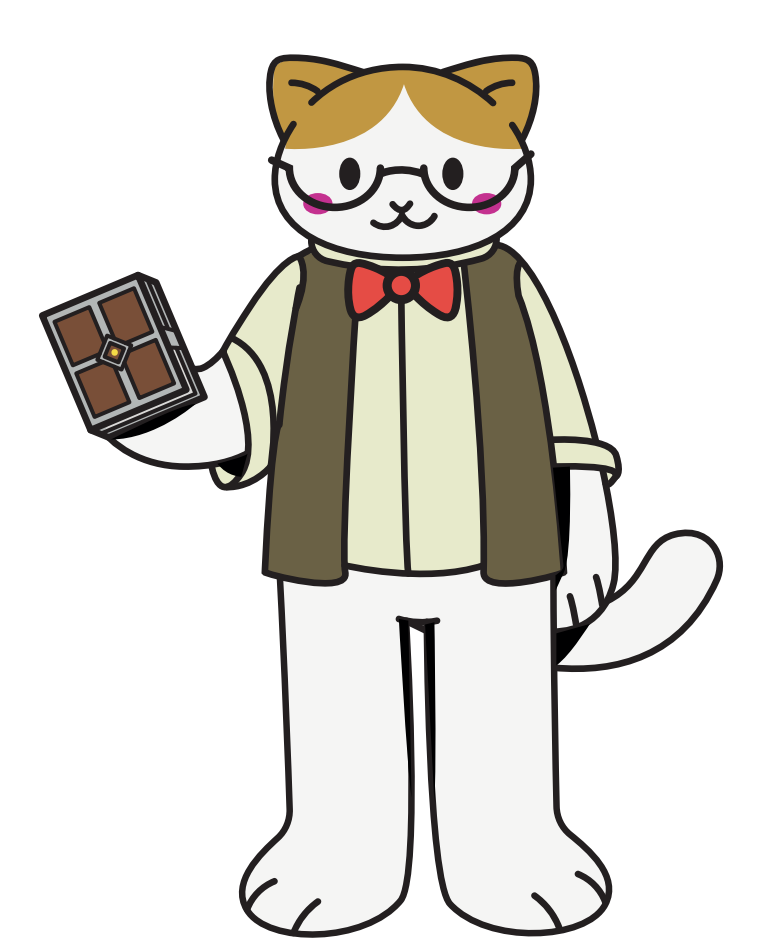
\includegraphics[scale=.33]{assets/01_gatito_introduccion.PNG}}       
\end{figure}



\bigskip

En el contexto de la computación, los lenguajes de programación fungen como una interfaz entre programador y procesador para establecer una comunicación sobre lo que queremos que la computadora ejecute por nosotros.\\\\
Diferentes paradigmas de lenguajes de programación, estilos, reglas y convenciones se han adoptado en las últimas décadas para ajustarse al mejor planteamiento posible de un problema, mantener un estándar declarativo, un nombramiento homogéneo de variables y métodos, o un estilo idéntico compartido entre los diferentes programas que se agrupan en estas categorías.\\\\
Iniciaremos el estudio de este manual planteando los conceptos claves que nos permitirán definir, clasificar y analizar a los lenguajes de programación que existen en el contexto de las ciencias de la computación. Estos conceptos nos permitirán definir nuestro propio lenguaje de programación desde cero.\\\\
Por último analizaremos sus propiedades y estudiaremos sus características más importantes para poder dar una implementación robusta aplicando las definiciones que iremos presentando en el desarrollo de esta introducción.\\

\subsection*{Objetivo}
    Comenzar el estudio formal de los lenguajes de programación brindando un primer acercamiento a la construcción básica de uno. Partiendo de las definiciones de los conceptos que componen un lenguaje, específicamente sintaxis, semántica, y pragmática. Así como a la clasificación que agrupa y distingue a los diferentes lenguajes computacionales en la actualidad\footnote{Para las personas que poseen una madurez matemática superior a aquella que la que un estudiante de cuarto semestre de la Facultad de Ciencias pudiera tener se recomienda encarecidamente iniciar el estudio de este manual en el \hyperref[sec:sintax]{capítulo 3: Sintaxis}. Los temas recomendados para omitir los primeros dos capítulos del manual son: estructuras discretas, juicios lógicos, reglas de inferencia e inducción estructural. }.

\subsection*{Planteamiento}
    Este capítulo inicia con el estudio de los lenguajes de programación, definiendo diferentes gramáticas para generar lenguajes pequeños y familiarizarnos con los elementos que los conforman.\\\\
    Es de particular interés analizar nuestro primer caso de estudio, el lenguaje \textsf{EAL}: Expresiones aritmético-lógicas proporcionando la gramática y esbozando como podemos interpretar las expresiones que pertenecen al mismo mediante la función de evaluación \texttt{eval}.\\\\
    Para cerrar el capítulo se discute brevemente la clasificación de los lenguajes de programación mas importantes de la actualidad basados en las características y paradigma de programación al que pertenecen. 

%    Sección 1: Composición de los lenguajes
\section{Las partes del lenguaje}

    La lingüística tiene como propósito definir una serie de reglas que rijan la estructura fundamental que compone un lenguaje.
Las reglas que estudian dicha composición pueden ser clasificadas en sintácticas (estructura gramatical), semánticas (significado) y pragmáticas (contexto de uso).\\

    % Ejercicio 1.2
    \begin{definition}(Sintaxis).
        En el contexto de las ciencias de la computación, la sintaxis de un lenguaje son las reglas que definen las combinaciones de símbolos que se consideran declaraciones o expresiones correctamente estructuradas\footnote{Definición extraída de  \hyperlink{29}{[29]}, \hyperlink{30}{[30]} y \hyperlink{31}{[31]}}.
        
    \end{definition}

\bigskip

    % Ejercicio 1.1
    \begin{definition}(Semántica).
        En el contexto de las ciencias de la computación, la semántica describe los procesos que sigue una computadora al ejecutar un programa en un lenguaje específico. Esto se puede mostrar describiendo la relación entre la entrada y la salida de un programa, o una explicación de cómo se ejecutará el programa en una determinada plataforma, creando así un modelo de cálculo\footnote{Definición extraída de \hyperlink{20}{[20]},  \hyperlink{21}{[21]} y \hyperlink{28}{[28]}}.
    \end{definition} 


    % Ejercicio 1.3
    \begin{definition}(Pragmática).
         En el contexto de las ciencias de la computación la pragmática se refiere a todos aquellos elementos del lenguaje que nos permiten obtener el significado de una expresión bajo un determinado contexto.\\\\
        Un ejemplo de esto son las bibliotecas, que nos permiten importar métodos previamente definidos. Así, la interpretación de una instrucción de esta biblioteca solo tiene un significado válido bajo el contexto que la importa\footnote{Extraído de \hyperlink{36}{[36]} y   \hyperlink{37}{[37]}}.
    \end{definition} 

    \bigskip

%    Sección 2: Gramática de los Lenguajes.
\section{Gramáticas y semántica de expresiones}

    Los lenguajes (no solo los de programación) requieren de un conjunto de reglas que nos permita formar las expresiones que pertenecen a ellos y un método de interpretación que nos diga el significado de las expresiones formadas a partir de dicho conjunto de reglas.\\\\
Las gramáticas de los lenguajes de programación consta de dos niveles: la sintaxis concreta y la sintaxis abstracta. Estudiaremos con especial atención la primera mientras que las sintaxis abstracta será presentada a detalle en el \hyperref[sec:sintax]{capítulo 3: Sintaxis}.\\\\
En cursos como autómatas y lenguajes formales\footnote{Conforme al plan de estudios que se imparte desde el 2013 en la Facultad de Ciencias de la Universidad Nacional Autónoma de México con clave de asignatura 1425. } se revisan este tipo de estructuras y las reglas que las generan, éstas usualmente son representadas como gramáticas libres de contexto. A continuación revisaremos algunos ejemplos aplicados para estructuras 
matemáticas.

	%ejercicio 2.1
	\begin{exercise}
        Dado el alfabeto $A=\{a, b\}$ define la gramática para generar $\{a^nb^n\ |\ n \in \N\}$\footnote{Ejercicio consultado de \hyperlink{135}{[135]}}. 
           \begin{align*}
				S & ::= aSb \ | \ \varepsilon 
			\end{align*}
    \end{exercise}

    % Ejercicio 2.2
    \begin{exercise}
        Define la gramática para generar n tal que, n $\in \ \N$\footnote{Ejercicio consultado de \hyperlink{134}{[134]}}. 
           \begin{align*}
				S & ::= BT \ | \ A \\
				T & ::= AT \ | \ A \\
				A & ::= B \ | \ 0 \\
				B & ::= 1 \ | \ 2 \ | \ 3 \ | \ 4 \ | \ 5 \ | \ 6 \ | \ 7 \ | \ 8 \ | \ 9
			\end{align*}
    \end{exercise}

	%ejercicio 2.3
	\begin{exercise}
        Define la gramática para generar expresiones aritméticas parentizadas con notación infija para el operador ''+''\footnote{Ejercicio consultado de \hyperlink{136}{[136]}}.  (puedes suponer definidos los números naturales a partir del ejercicio anterior)\footnote{Aquí hacemos abuso de la notación en la última regla puesto que $\N$ no es un elemento de la gramática por si mismo, este hace referencia a los número naturales generados del ejercicio 2.2.}.
			 \begin{align*}
				S & ::= S \ + \ A \ | \ A \\
				A & ::= (S) \ | \ \N
			\end{align*}
    \end{exercise}



%https://cs.stackexchange.com/questions/97794/what-is-a-non-ambiguous-cfg-for-generating-the-set-of-natural-numbers

%https://repositorium.sdum.uminho.pt/bitstream/1822/53514/1/OASIcs-SLATE-2016-10.pdf

%https://web.stanford.edu/class/archive/cs/cs103/cs103.1164/lectures/18/Slides18.pdf

%https://www.cs.bu.edu/fac/snyder/cs320/Review%20and%20Practice%20Problems/Practice%20Problems%2007.html


\subsection{El lenguaje EAL}

	Vamos a definir la base del lenguaje que utilizaremos para el resto del manual, este  se denomina \textsf{EAL} (expresiones aritméticas y lógicas). Poco a poco iremos extendiendo y agregando instrucciones para hacerlo más robusto, por el momento nos limitaremos a definir los operadores aritméticos básicos: ''+'', ''-'',''*'' y los operadores lógicos: ''$<$'', ''isZero'' y ''not''. De igual forma definimos las constantes \texttt{true}, \texttt{false} y los números naturales. 
    % Definición del lenguaje EAB
    \begin{definition}[Sintaxis de {\sf Expresiones aritmético-lógicas: EAL}]
        \[
            \begin{array}{rll}
                e & ::= &  n\quad |\quad {\tt true}\quad |\quad {\tt false}\quad |\quad e + e\quad |\quad e - e\quad |\quad e*e\quad |\quad e<e\quad 
            \end{array}
       \]
       \[
	 \begin{array}{rll}
		|\quad {\tt isZero}\;e\quad |\quad {\tt not}\;e
	\end{array}
        \]
        Nuevamente hacemos abuso en la notación para $n$, en donde $n\in\mathbb{N}$\footnote{Definición formulada de  \hyperlink{1}{[1]},  \hyperlink{5}{[5]}.  \hyperlink{12}{[12]},  \hyperlink{26}{[26]} y  \hyperlink{39}{[39]}.}.
    \end{definition}
        
    % Definición de la función semanticá para EAB
    \begin{definition}[Semántica de \textsf{EAL}] Función de evaluación para el lenguaje de expresiones aritmético-lógicas.
        $$\llbracket\cdot\rrbracket:{\sf EAL}\to\mathbb{N} \cup \textit{Bool}$$
         Esto quiere decir que la función de evaluación recibe una expresión del lenguaje \textsf{EAL} y regresa un número natural ó un booleano
        \[
            \begin{array}{rll}
                \llbracket n\rrbracket&=&n\\
                \llbracket {\tt true}\rrbracket&=&{\tt true}\\
                \llbracket {\tt false}\rrbracket&=&{\tt false}\\
                \llbracket e_1 + e_2\rrbracket&=&\llbracket e_1\rrbracket+_\mathbb{N}\llbracket e_2\rrbracket\\
 \llbracket e_1 - e_2\rrbracket&=&\llbracket e_1\rrbracket-_\mathbb{N}\llbracket e_2\rrbracket\\
                \llbracket e_1*e_2\rrbracket&=&\llbracket e_1\rrbracket\times_\mathbb{N}\llbracket e_2\rrbracket\\
                \llbracket e_1<e_2\rrbracket&=&\llbracket e_1\rrbracket<_\mathbb{N}\llbracket e_2\rrbracket\\
                \llbracket {\tt isZero}\;e\rrbracket&=&{\sf zero}_\mathbb{N}\llbracket e\rrbracket\\
                \llbracket {\tt not}\;e\rrbracket&=&\lnot\llbracket e\rrbracket
            \end{array}
        \]
        En donde $ n \in \mathbb{N}$ y las constantes $\tt false$, $\tt true \in $ $Bool$.\\
        Los operadores $+_\mathbb{N},\times_\mathbb{N},<_\mathbb{N}$ y ${\sf zero}_\mathbb{N}$ representan las funciones de suma, producto, menor que y el \textit{test} de cero definidas para los naturales respectivamente, mientras que $\lnot$ es la negación lógica para $Bool$\footnote{Definición extraída de \hyperlink{1}{[1]},  \hyperlink{5}{[5]}.  \hyperlink{12}{[12]},  \hyperlink{26}{[26]} y  \hyperlink{39}{[39]}.}.
    \end{definition}

    A partir de la definición anterior se puede implementar un intérprete para expresiones del lenguaje \textsf{EAL} mediante una función recursiva $\tt eval$ como sigue:
    \vskip 1em
    \begin{lstlisting}
        eval n          = n
        eval true       = true
        eval false      = false
        eval (e1 + e2)  = eval e1 + eval e2
        eval (e1 - e2)  = eval e1 - eval e2
        eval (e1 * e2)  = eval e1 * eval e2
        eval (e1 < e2)  = (eval e1) < (eval e2)
        eval (not e)    = not (eval e)
        eval (iszero e) = (eval e) == 0
     \end{lstlisting}

    Con esta definición ahora podemos evaluar algunas expresiones pertenecientes a nuestro lenguaje \textsf{EAL}.

    % Ejercicio 2.4
    \begin{exercise}
        Evalúa la expresión: \texttt{not} 3 $\textless$ 5 + 7  haciendo uso de la implementación del intérprete anteriormente definido para \textsf{EAL}.
        \vskip 1em
        \begin{lstlisting}
                eval(not 3 < 5 + 7)  =   	                                                                
                not(eval(3 < 5 + 7))  =          	                                                               
                not(eval(3) < eval(5 + 7))  =
                not(eval(3) <  eval(5) + eval(7)) =   
                not(3 < 5 + 7)  =                                                                            
                not(3 < 12)  =               	                                                                                                 
                not(true)  =
                false
        \end{lstlisting}
        
    \end{exercise}


    % Ejercicio 2.5
    \begin{exercise}
        Evalúa la expresión: $3$ * $\texttt{true}$ $ \textgreater$  $8$  haciendo uso de la implementación del intérprete anteriormente definido para \textsf{EAL}.
        \vskip 1em
        \begin{lstlisting}
            eval(3 * true > 8)        =                              
            eval(3 * true) > eval(8)  =            
            eval(3) * eval(true) >  8 =                                                  
            3 * true > 8              
        \end{lstlisting}
        En este caso, aún cuando la expresión \textsf{EAL} está bien formada, no existe una regla en nuestro intérprete que nos permita evaluar más, por lo tanto esta expresión no tiene resultado. Más adelante estudiaremos mecanismos para evitar que casos como este figuren en la evaluación de un lenguaje.

    \end{exercise}

    \begin{definition}
        Sea \textit{G} una gramática libre de contexto, decimos que que \textit{G} es una gramática ambigua si existe una cadena para la cual se pueda tener más de una derivación a la izquierda\footnote{Definición extraída de \hyperlink{5}{[5]}. \hyperlink{12}{[12]}, \hyperlink{40}{[40]} y \hyperlink{41}{[41]}.}.
    \end{definition}


    \begin{exercise}
        ¿La gramática definida para \textsf{EAL} es ambigua? Argumenta tu respuesta.                          \\
             Sí porque podemos derivar de dos formas distintas la cadena: $3 + 4 * 5$                            
             \begin{center}
                 \textit{e} $\rightarrow$ \\
                 \textit{e} + \textit{e} $\rightarrow$ \\
                 3 + \textit{e} $\rightarrow$ \\
                 3 + \textit{e} * \textit{e} $\rightarrow$ \\
                 3 + 4 * \textit{e} $\rightarrow$ \\
                 3 + 4 * 5.  \\
                 
                 \bigskip
                 
                 \textit{e} $\rightarrow$ \\
                 \textit{e} * \textit{e} $\rightarrow$ \\
                 \textit{e} * 5 $\rightarrow$ \\
                 \textit{e} + \textit{e} * 5 $\rightarrow$ \\
                 \textit{e} + 4 * 5 $\rightarrow$ \\
                 3 + 4 * 5.
             \end{center}
    \end{exercise}

    \bigskip

    % Ejercicio 2.7
    \begin{exercise}
        ¿Cómo eliminarías la ambigüedad de esta gramática?    \\\\                    
            Con la introducción de paréntesis para marcar la precedencia de las operaciones. 
            En el ejemplo anterior la ambigüedad queda eliminada en su totalidad:
            \begin{center}
                $(3 + (4 * 5))$  ó $((3 + 4 )* 5)$
            \end{center}
    \end{exercise}


% Sección 3: Clasificación de los lenguajes.
\section{Clasificación de los lenguajes de programación}

    En computación existen diferentes clasificaciones que nos permiten agrupar lenguajes según sus características principales, paradigma de programación al que pertenecen, tecnología involucrada en el proceso de traducción a lenguaje de máquina, etc. A continuación se enlistan algunas de estas categorías: 

    \begin{itemize}
        \item Lenguajes compilados,  que como el nombre lo indica precisan de un compilador para traducir el código de alto nivel a instrucciones de máquina que el procesador pueda ejecutar. Generalmente suelen ser mas lentos al momento de ejecutarse que el resto de las categorías  ya que requieren de un sistema sofisticado de inferencia de tipos, optimizaciones en la traducción de las instrucciones y en ocasiones entornos especiales para la ejecución de los programas como la máquina virtual de Java (\textit{JVM} por sus siglas en inglés)\footnote{Información obtenida de \hyperlink{43}{[43]}, \hyperlink{44}{[44]}, \hyperlink{45}{[45]}, \hyperlink{46}{[46]}}.\\

        \item Lenguajes interpretados, en donde las instrucciones son mapeadas a su traducción equivalente en el lenguaje de máquina cuando la línea que contiene dicha instrucción se vaya a ejecutar por el procesador\footnote{También es posible interpretar las expresiones de un lenguaje como el valor asociado a dicha expresión una vez que se evalúa. En este curso estudiaremos este proceso en el \hyperref[sec:semantics]{capítulo 4: Semántica}.}. Generalmente son menos robustos a la hora de encontrar errores de tipo, errores en la tipografía, caracteres faltantes, etc. Sin embargo este tipo de lenguajes de programación resultan particularmente útiles por que permiten el modelado y la realización de programas mucho más rápido que los lenguajes compilados\footnote{Información obtenida de \hyperlink{43}{[43]}, \hyperlink{44}{[44]}, \hyperlink{45}{[45]}, \hyperlink{46}{[46]}}.\\

        \item También se pueden clasificar por paradigma como en el caso de los lenguajes funcionales que se enfocan en la especificación de un problema mediante condiciones en lugar de la solución teniéndose la siguiente definición: 
         ''La programación funcional es un paradigma de programación en el que los programas se construyen aplicando y componiendo funciones. Íntimamente relacionado con el paradigma de programación declarativa en el que las definiciones de funciones son árboles de expresiones que asignan valores a otros valores, en lugar de una secuencia de declaraciones imperativas que actualizan el estado de ejecución del programa. ''\footnote{Definición extraída de \hyperlink{51}{[51]} y \hyperlink{52}{[52]}}\\

        \item  La programación imperativa contrasta con la clasificación anterior por su naturaleza secuencial, podemos encapsular sus características más importantes en la siguiente definición: 
         ''Un paradigma de programación de software que utiliza declaraciones que cambian el estado de un programa. De la misma manera que el modo imperativo en los lenguajes naturales expresa órdenes, un programa imperativo consta de órdenes que debe ejecutar la computadora. La programación imperativa se centra en describir cómo funciona un programa paso a paso\footnote{[\hyperlink{53}{[53]}} en lugar de descripciones de alto nivel de sus resultados esperados. ''\footnote{Extraído de \hyperlink{53}{[53]}, \hyperlink{54}{[54]}, \hyperlink{55}{[55]} y \hyperlink{56}{[56]}}\\\\
        El término se utiliza con frecuencia como un contrapunto de la programación declarativa, siendo el primero un conjunto de instrucciones para solucionar un determinado problema mientras que el segundo se centra en la especificación del problema mismo.\\

        \item     Otra clasificación que es muy socorrida en la computación es la llamada orientada a objetos que modela las entidades de un programa con su identidad, métodos, variables y que brindan características deseables como la herencia, el polimorfismo y el encapsulamiento de datos.\\\\
        Esta clasificación pertenece al paradigma imperativo dado que se trabaja estrechamente con el estado del programa en cada paso de la ejecución, sus direcciones de memoria y sus sentencias de control\footnote{Definición extraída de \hyperlink{47}{[47]}, \hyperlink{48}{[48]}, \hyperlink{49}{[49]}}.\\
    
        \item     Por último mencionaremos brevemente la clasificación de los lenguajes lógicos. Los programas que pertenecen a esta categoría se pueden definir de la siguiente forma:  ''Un programa, base de datos o base de conocimientos en un lenguaje de programación lógica es un conjunto de oraciones en forma lógica que expresan hechos y reglas sobre un dominio específico. ''\footnote{Definición extraída de \hyperlink{57}{[57]}} \\\\
        Generalmente este tipo de programas se apoyan definiendo predicados y objetos a los cuales estos predicados pueden ser aplicados así como instrucciones y operadores lógicos para dar solución a los problemas planteados en este modelo.

    
    \end{itemize}

    \bigskip

    % Ejercicio 3.3
    %\begin{exercise}
    %    Elabora un mapa mental con las características y clasificaciones que consideres más importante en los lenguajes de programación.
    %    \begin{figure}[htbp]
    %        \centerline{\includegraphics[scale=.45]{mapa.jpg}}
    %        \label{fig 1. Mapa para clasificar los lenguajes de programación.}
    %    \end{figure}
    %\end{exercise}

    %\begin{figure*}[ht]
    %    \centering
    %\end{figure*}
   %(Imagen de José M. Barranco:  ''Mapa Mental: Lenguajes de Programación) ''

    \bigskip
    \bigskip

 % Ejercicio 3.1
    \begin{exercise}
        Da una implementación del algoritmo \texttt{selectionSort} en programación imperativa.

	\begin{lstlisting}[language=C++]
	void swap(int *xp, int *yp){
	    int temp = *xp;
	    *xp = *yp;
	    *yp = temp;
	}
	 
	void selectionSort(int arr[], int n){
	    int i, j, min_idx;
	    for (i = 0; i < n-1; i++){
	        min_idx = i;
	        for (j = i+1; j < n; j++)
	        if (arr[j] < arr[min_idx])
	            min_idx = j;
	        swap(&arr[min_idx], &arr[i]);
	    }
	}
	 
	\end{lstlisting}
    \end{exercise}

      % Ejercicio 3.2
    \begin{exercise}
        Da una implementación del algoritmo \texttt{selectionSort} en programación declarativa.
	\begin{lstlisting}[language=Haskell] import Data.List (minimum, delete)
		ssort :: Ord t => [t] -> [t]
		ssort [] = []
		ssort xs = let { x = minimum xs } 
		           in  x : ssort (delete x xs)
	\end{lstlisting}
    \end{exercise}


% Ejercicios a discresión del lector   
\section{Ejercicios para el lector}

    % Ejercicio 4.1
    \begin{exercise}
        El uso del carácter especial ';' al terminar una instrucción de programa en lenguajes de programación como \textsf{C} y \textsf{Java} ¿a qué tipo de regla corresponde (sintáctica, semántica o pragmática)?
    \end{exercise}

\bigskip

    % Ejercicio 4.2
    \begin{exercise}
        Ejemplifica la aplicación de la pragmática aplicada en el contexto de los lenguajes de programación.
    \end{exercise}

\bigskip

     % Ejercicio 4.3
    \begin{exercise}
        En el contexto de los lenguajes de programación muchas veces la semántica de una expresión es explicada en lenguaje natural en la documentación del lenguaje. \\\\
        Explica por qué esto no es una semántica formal.
    \end{exercise}

\bigskip

    % Ejercicio 4.4
    \begin{exercise}
        Escribe una gramática para el alfabeto $\Sigma = \{a,b\}$ y el lenguaje
        \[L=\{a^n b^m\ \textbar\ n \textgreater 0, m \geq n \}\]
    \end{exercise}

\bigskip

     % Ejercicio 4.5
    \begin{exercise}
        Escribe una gramática para el alfabeto $\Sigma = \{a,b\}$ y el lenguaje  
        \[L= \text{cadenas palíndromas} \]
    \end{exercise}

\bigskip
    % Ejercicio 4.6
    \begin{exercise}
        Escribe una gramática para el alfabeto  $\Sigma = \{(,)\}$ y el lenguaje \[ L= \text{cadenas de paréntesis balanceados} \]
    \end{exercise}

\bigskip

    % Ejercicio 4.7
    \begin{exercise}
        Evalúa la expresión del lenguaje \textsf{EAL} utilizando la función \texttt{eval}. \\ \\ 
        $$7 * 8 < 3 * 9$$
    \end{exercise}

\bigskip

    % Ejercicio 4.8
    \begin{exercise}
        Evalúa la expresión del lenguaje \textsf{EAL} utilizando la función \texttt{eval}. \\ \\
            $$\texttt{not(iszero}( (7 * 4) + (1 * 0)))$$
    \end{exercise}

\bigskip

    % Ejercicio 4.9
    \begin{exercise}
        Escribe el algoritmo de la búsqueda binaria en un arreglo ordenado en el paradigma de programación imperativo.
    \end{exercise}
\bigskip
    % Ejercicio 4.10
    \begin{exercise}
        Escribe el algoritmo de la búsqueda binaria en un arreglo ordenado en el paradigma de programación declarativo.
    \end{exercise}

% https://opendsa-server.cs.vt.edu/OpenDSA/Books/PIFLAS21/html/IntroGrammarEx.html
% https://programming-idioms.org/idiom/124/binary-search-for-a-value-in-sorted-array/2120/haskell
% https://www.geeksforgeeks.org/binary-search/

% https://www.seas.upenn.edu/~cis1940/spring13/hw/01-intro.pdf
% https://wiki.haskell.org/Typeclassopedia
% https://github.com/JD95/haskell-problem-sets/blob/master/Lists/Problems.hs
% https://www.reddit.com/r/haskell/comments/evlmsr/beginner_exercises/

    %https://tex.stackexchange.com/questions/669517/notes-at-the-end-of-the-book-document-what-is-the-modern-way-of-doing-it
		
		\chapter{Herramientas matemáticas}
			
%    Segundo capítulo: Herramientas Matemáticas.
%    Ejercicios por Barón M. Miguel.
%    Teoría por Javier Enríquez Mendoza.
%    Empezado el 21/10/22
%    Concluido el 25/10/22

%Gatito Constructor
\begin{figure}[htbp]
    \centerline{
\includegraphics[scale=.19]{assets/02_gatito_herramientas_matematicas.jpg}}
    \label{fig 1. Mapa para clasificar los lenguajes de programación.}        
\end{figure}

Para estudiar a los lenguajes de programación es necesario definir una estructura que nos permita capturar su esencia matemática y nos proporcione un mecanismo para demostrar características y propiedades asociadas a estos. \\\\
Una manera de definir formalmente un lenguaje de programación es mediante el uso de juicios lógicos\footnote{En lógica el equivalente a un juicio lógico son los predicados que denominan una característica que se cumple en una proposición.} para definir propiedades, pertenencia de los elementos de nuestra estructura a un conjunto, relación entre diferentes elementos de una misma estructura, etc\footnote{Para las personas que poseen una madurez matemática superior a aquella que la que un estudiante de cuarto semestre de la Facultad de Ciencias pudiera tener se recomienda encarecidamente iniciar el estudio de este manual en el \hyperref[sec:sintax]{capítulo 3: Sintaxis}. Los temas recomendados para omitir los primeros dos capítulos del manual son: estructuras discretas, juicios lógicos, estructuras recursivas, reglas de inferencia e inducción estructural. }. \\
\subsection*{Objetivo}
Estudiar las estructuras matemáticas que utilizaremos para familiarizarnos con el concepto de inducción estructural. En particular centraremos nuestra atención a estructuras recursivas como listas de tipo A y árboles binarios balanceados de tipo A\footnote{donde A es un conjunto o una colección de elementos.} junto con las reglas que nos permiten construir estas estructuras.\\\\
Este tipo de mecanismos es particularmente útil para ilustrar las propiedades de los lenguajes que definiremos a lo largo de los capítulos de este manual.

\subsection*{Planteamiento}
En este capítulo exploraremos diferentes estructuras empezando por los juicios lógicos que constituyen las entidades fundamentales sobre las cuales iniciaremos el estudio de los lenguajes.
También estudiaremos brevemente estructuras recursivas como cadenas y listas para enunciar el principio de inducción que nos permite demostrar propiedades sobre dichas estructuras. Por último estudiaremos un sistema de transición para modelar los estados y reglas de evaluación de la instancia de un juego.

%    Sección 1: Juicios lógicos.
\section{Juicios lógicos}

    Una parte fundamental del razonamiento matemático es la capacidad de determinar si una afirmación es verdadera o falsa basado en la información que poseemos sobre los elementos que son mencionados en dicha afirmación. \\\\
    Para poder aplicar un juicio sobre algún elemento, objeto o entidad para determinar su veracidad primero debemos definir dichos elementos. A continuación vamos a introducir los conceptos necesarios para poder formalizar esta noción y como aplicarla. Esto será de utilidad para definir características, reglas de construcción y reglas de evaluación en los lenguajes de programación y modelos de computo que discutiremos a lo largo del manual.\\

    \bigskip

    % Ejercicio 1.1
    \begin{exercise}
	¿Qué es una entidad matemática? \\  \\
	   ''En el lenguaje habitual de las matemáticas, una entidad es cualquier cosa que ha sido (o podría ser) definida formalmente y con la que se pueden realizar razonamientos deductivos y pruebas matemáticas. ''\footnote{Definición formulada de \hyperlink{58}{[58]}, \hyperlink{59}{[59]} y \hyperlink{60}{[60]}}
    \end{exercise}

    % Ejercicio 1.2
    \begin{exercise}
	¿Qué es un juicio? \\ \\
         ''En lógica matemática, un juicio es una afirmación o enunciación de una característica o propiedad sobre un objecto o elemento de un dominio. ''\footnote{Definición formulada de \hyperlink{61}{[61]} y \hyperlink{62}{[62]}.}
    \end{exercise} 

    % Ejercicio 1.3
    \begin{exercise}
	Proporciona un listado de juicios sobre objetos matemáticos (Puedes suponer definidos con anterioridad elementos como $\mathbb{N}$, $\mathbb{Q}$, Bool, \textit{String}, funciones, relaciones de orden, operadores aritméticos, etc).
	\begin{center}
		\begin{tabular}{rl}
			 ''Hola Mundo'' \textbf{$String$} & La cadena  ''Hola Mundo'' es de tipo $String$.  \\
			L \textbf{$NP$} & El lenguaje L es $NP$. \\
			\textit{a} $\textgreater$ \textit{b} & el número $a$ es más grande que el número $b$. \\
			A $|$ B  & El evento A es independiente al evento B. \\
			\textit{True} Bool  & La constante \textit{True} es de tipo Bool.  \\
			h = \( g \circ f \) & la función $h$ es la composición de la función $g$ con la función $f$.\\
			3.1416... $\mathbb{I}$ & El número 3.1416... es  irracional \\
			0 $\mathbb{N}$  & 0 es un Natural. \\
			S(0) impar & El sucesor de 0 es impar.\\
			$\frac{p}{q}$  $\mathbb{Q}$  & La fracción $\frac{p}{q}$ es un racional.\\
			...
		\end{tabular}
	\end{center}
    \end{exercise}

%    Sección 2: Reglas de Inferencia, Inducción estructural.
\section{Reglas de inferencia}

    Las reglas de inferencia\footnote{En esta manual utilizaremos el término  ''regla de inferencia '' o  ''juicio lógico '' de forma indistinta.} son una representación de la aplicación de un juicio de la forma:  ''Si las premisas $p_1,p_2,\ ...\ p_n$ son verdaderas, entonces $c$ es verdadero .'' Visualmente esto se denota como:
    \[
        \inference{p_1,p_2,\ ...\ p_n}{\textit{c}}
    \]
    Podemos observar que las reglas de inferencia están compuestas por dos secciones: una sección superior y una inferior. 
    La sección superior es en donde se agrupan las condiciones necesarias para que la regla pueda ser aplicada (a los elementos enlistados en esta parte se les conoce como premisas o hipótesis), cada una de estas están separadas por una coma (',') y todas deben de cumplirse\footnote{El signo de puntuación (',') se puede interpretar como el operador $\wedge$ donde cada hipótesis es un argumento de dicho operador.}. \\\\
    La sección inferior de una regla de inferencia enlista el resultado de la aplicación de la regla a las premisas. Ocasionalmente la regla tendrá un nombre que ayuda a identificar cuál de ellas es aplicada cuando se trabaja con derivaciones y razonamientos\footnote{Definición formulada de \hyperlink{1}{[1]}, \hyperlink{5}{[5]}, \hyperlink{9}{[9]}, \hyperlink{63}{[63]}, \hyperlink{64}{[64]} y \hyperlink{91}{[91]}.}. En esta sección de la regla puede haber uno o más elementos resultados de la aplicación pero no puede ser vacía. \\\\
    Los axiomas son las reglas de inferencia que carecen de hipótesis dado que siempre serán verdad y no es necesario suponer nada para concluirlas.\\\\
    Tomemos como ejemplo la definición de las cadenas binarias de tipo A (denominaremos a este tipo de dato como A*) para ilustrar las reglas de inferencia y sus partes anteriormente discutidas.

    \bigskip

    % Definición: Cadenas Binarias y función de concatenación.
    \begin{definition}
        Sea $\text{A} = \{ 0,1 \}$ un conjunto. Definimos el tipo de dato recursivo $\text{A}^*$ (cadenas binarias de tipo A)\footnote{Definición formulada a partir de \hyperlink{67}{[67]}, \hyperlink{68}{[68]} y \hyperlink{69}{[69]}} como sigue: \\
            \[
                \begin{array}{lcl}    
                    \inference{}{\varepsilon \in \text{A}^*}[\textit{(eps)}] \qquad 
                    \inference{a \in \text{A},\; s \in \text{A}^*}{\<a, s\> \in \text{A}^*}[\textit{(tup)}]
                \end{array}
            \] 


            La regla \textit{eps} se lee como:  ''la cadena vacía es una cadena binaria de tipo A.'' Nótese que esta regla es un axioma dado que carece de premisas. \\\\
            La regla \textit{tup} se lee como:  ''si \textit{a} es de tipo A y \textit{s} es una cadena binaria de tipo A, entonces la construcción de una tupla con cabeza \textit{a} y cola \textit{s} es una cadena binaria de tipo A.''\\\\
            Por ejemplo, la cadena 10101 se representa por la 5-tupla $\<1,\<0,\<1,\<0,\<1. \epsilon \>\>\>\>\>$ 
    \end{definition}

    \bigskip

\section{Estructuras recursivas e inducción estructural}

    Ahora discutamos un tipo de estructuras particulares que se relacionan de forma íntima con los conceptos anteriormente planteados; las estructuras recursivas\footnote{Definición formulada a partir de \hyperlink{91}{[91]}, \hyperlink{92}{[92]} y \hyperlink{93}{[93]}}. Estas se generan a partir de dos casos:
    \begin{itemize}
 
        \item La estructura está compuesta por el elemento más primitivo que puede formar parte de esta.
        Muchas veces este elemento constituye la clausula de escape para la recursión inducida por la definición y constituiría un axioma en su representación como regla de inferencia.
        \item La estructura está compuesta por una llamada a la función constructora con un elemento nuevo y la estructura misma que se desea definir como argumentos. 
    \end{itemize}


    En el caso del tipo de dato A*, el elemento más primitivo que pertenece a esta estructura es la cadena vacía (denotada como $\varepsilon$) o bien una tupla con cabeza \textit{a} $\in $ A y cola de tipo A*.\\\\
    Este principio se aplica tanto para definir la estructura recursiva como para las funciones que se quieran aplicar sobre la misma\footnote{Información obtenida de \hyperlink{94}{[94]} y \hyperlink{95}{[95]}}. Para ilustrar este punto definimos la función para concatenar dos elementos de A* de la siguiente forma: 
    \begin{definition}
        Definimos la concatenación de cadenas A* denotada como: $\bullet$ ::\ (A* $\rightarrow$\ A*) $\rightarrow$\ A* mediante la siguiente especificación\footnote{Definición formulada a partir de \hyperlink{67}{[67]}, \hyperlink{68}{[68]}}:
        \[
            \begin{array}{rcl}
                \text{Caso base:}   & \varepsilon \bullet t  =   t &  (\textit{eps}) \\
                \text{Constructor:} & \<a,s\> \bullet t  =  \<a,\<s \bullet t\>\> & (\textit{tup})
            \end{array}
        \]
    \end{definition}
    La característica mas importante que las estructuras recursivas poseen es el principio de inducción. Esta propiedad nos permite demostrar que una proposición o propiedad es válida para cualquier elemento de la estructura mediante su aplicación de la siguiente forma:
    \begin{itemize}
        \item Se demuestra la validez de la proposición para los elementos primitivos.
        \item Posteriormente se asume que la propiedad es válida para cualquier instancia. 
        \item Por último se demuestra la propiedad aplicada para los constructores que generan instancias más grandes aplicando la hipótesis del inciso anterior.
    \end{itemize}

    \bigskip

    % Ejercicio 2.1
    \begin{exercise}
        Utiliza la inducción estructural para demostrar: 
        \[ t \bullet \varepsilon = t\] 
            \textbf{Caso Base} t = $\varepsilon$ \\
            $\varepsilon \bullet \varepsilon$ =  $\varepsilon$ \qquad \qquad \qquad \qquad \qquad \qquad \qquad \qquad \qquad \qquad \qquad \quad (Por la definición de $\bullet$) \\
            $\varepsilon$ = $t$. \\\\
            \textbf{Hipótesis Inductiva} $t \bullet \varepsilon = t$  para toda $t \in \text{A}^*$ \\\\
            \textbf{Paso Inductivo} por demostrar $\<a,t\> \bullet \varepsilon = \<a,t\>$ para toda $a \in \text{A}$ y $t \in \text{A}^*$ \\
            $\<a,t\> \bullet \varepsilon$ = $\<a, \<t \bullet \varepsilon \> \>$ \qquad \qquad \qquad \qquad \qquad \qquad \qquad \qquad \quad \quad (Por la definición de $\bullet$) \\
            $\<t \bullet \varepsilon \> = t $ \qquad \qquad \qquad \qquad \qquad \quad \qquad \qquad \qquad \qquad \qquad\ (Por la hipótesis inductiva) \\
            $\<a,t\> \bullet \varepsilon = \<a, \<t \bullet \varepsilon \> \> = \<a, t\>$ \\ 
    \end{exercise}


    % Ejercicio 2.2
    \begin{exercise}
        utiliza las reglas (\textit{eps}) y (\textit{tup}) para derivar las cadenas: 
        \[
             \<1,\<0,\<0,\varepsilon\>\>\>, \qquad
             \<1,\<0,\<0\<1,\varepsilon\>\>\>\> \qquad y \qquad
             \<1,\<1,\<1,\<0,\<1,\<0,\varepsilon\>\>\>\>\>\>
        \] 

        \bigskip

        \scalemath{0.9}{
            \begin{array}{cc}
                \inference{\inference{}{1 \in \text{A}}[(\textit{ax})] \inference{\inference{}{0 \in \text{A}}[(\textit{ax})]& \inference{\inference{}{0 \in \text{A}}[(\textit{ax})]& \inference{}{\varepsilon \in \text{A}^*}[(\textit{eps})]}{\<0, \varepsilon \> \in \text{A}^*}[(\textit{tup})]}{\<0,\<0,\varepsilon\>\> \in \text{A}^*}[(\textit{tup})]}{\<1,\<0,\<0,\varepsilon\>\>\> \in \text{A}^*}[(\textit{tup})]
            \end{array}
        }

    \bigskip

        \scalemath{0.7}{
            \begin{array}{cc}
                \inference{\inference{}{1 \in \text{A}}[(\textit{ax})]& \inference{\inference{}{0 \in \text{A}}[(\textit{ax})]& \inference{\inference{}{0 \in v}[(\textit{ax})]& \inference{\inference{}{1 \in \text{A}}[(\textit{ax})]& \inference{}{\varepsilon \in \text{A}}[(\textit{eps})]}{\<1,\varepsilon\> \in \text{A}^*}[(\textit{tup})]}{\<0\<1,\varepsilon\>\> \in \text{A}^*}[(\textit{tup})]}{\<0,\<0\<1,\varepsilon\>\>\> \in \text{A}^*}[(\textit{tup})]}{\<1,\<0,\<0\<1,\varepsilon\>\>\>\> \in \text{A}^*}[(\textit{tup})]
            \end{array}     
        }

    \bigskip

        \scalemath{0.49}{
            \begin{array}{cc}
                \inference{\inference{}{1 \in \text{A}}[(\textit{ax})] \inference{\inference{}{1 \in \text{A}}[(\textit{ax})]&  \inference{\inference{}{1 \in \text{A}}[(\textit{ax})]&  \inference{\inference{}{0 \in \text{A}}[(\textit{ax})]&  \inference{\inference{}{1 \in \text{A}}[(\textit{ax})]& \inference{\inference{}{0 \in \text{A}}[(\textit{ax})]& \inference{}{\varepsilon \in \text{A}^*}[(\textit{eps})]}{\<0,\varepsilon\> \in \text{A}^*}[(\textit{tup})]}{\<1,\<0,\varepsilon\>\> \in \text{A}^*}[(\textit{tup})]}{\<0,\<1,\<0,\varepsilon\>\>\> \in \text{A}^*}[(\textit{tup})]}{\<1,\<0,\<1,\<0,\varepsilon\>\>\>\> \in \text{A}^*}[(\textit{tup})]}{\<1,\<1,\<0,\<1,\<0,\varepsilon\>\>\>\>\> \in \text{A}^*}[(\textit{tup})]}{ \<1,\<1,\<1,\<0,\<1,\<0,\varepsilon\>\>\>\>\>\> \in \text{A}^*}[(\textit{tup})]
            \end{array}  
        }
    \end{exercise}


    % Definición 2.2: Función para contar caracteres
    \begin{definition}
        Definimos la función para contar caracteres\footnote{Definición formulada a partir de \hyperlink{67}{[67]}, \hyperlink{68}{[68]} y \hyperlink{69}{[69]}} en una cadena denotada por $n_c$ :: A* $\rightarrow$ Int como sigue:
        \[   
            n_c(\<a,t\>) = 
                \begin{cases}
                    n_c(\varepsilon) = 0 \\
                    1 + n_c(t) & \text{Sí \textit{a} = c} \\
                    n_c(t)     & \text{Sí \textit{a}} \neq c \\
                 \end{cases}
        \]
    \end{definition}

    \bigskip

    % Ejercicio 2.3
    \begin{exercise}
        Utiliza la inducción estructural para demostrar

           \[ n_c(s \bullet t) = n_c(s) + n_c(t)  \]

        \textbf{Caso Base} $s = \varepsilon$ \\\
             $n_c(\varepsilon \bullet t) = n_c(t)$ \qquad \qquad \qquad \qquad \qquad \qquad \qquad \qquad \qquad \qquad \quad (Por la definición de $\bullet$)\\
             = $0 + n_c(t)$ = $n_c(\varepsilon) + n_c(t)$ \qquad \qquad \qquad \quad \qquad \qquad \qquad  \qquad\  (Por la definición de $n_c$)\\
             = $n_c(s) + n_c(t)$\\

        \textbf{Hipótesis Inductiva}  $n_c(s \bullet t) = n_c(s) + n_c(t) $ \\

        \textbf{Paso Inductivo} Por demostrar para $s = \<a,s'\>$\\
            $n_c(\<a,s'\> \bullet t)$ = $n_c(\<a, s' \bullet t \>)$ \qquad \qquad \qquad \qquad \qquad \qquad \qquad \quad (Por la definición de $\bullet$)\\
            
        \textbf{Caso 1} $a = c$ entonces tenemos\\
            = $n_c(\<a, s' \bullet t \>)$ = $1 + n_c( s' \bullet t ) $ \qquad \qquad \qquad \qquad \qquad \quad \quad \quad\ (Por la definición de $n_c$) \\
            = $1 +  n_c(s') +  n_c(t)$ \qquad \qquad \qquad \qquad \qquad \qquad \qquad \qquad \quad (Por la hipótesis inductiva) \\
            = $(1 + n_c(s')) + n_c(t)$ = $n_c(\<a,s'\>) +  n_c(t)$ \qquad \qquad \qquad \quad \quad\ (Por la definición de $n_c$) \\

        \textbf{Caso 2} $a \neq c$ entonces tenemos \\
            = $n_c(\<a, s' \bullet t \>)$ = $n_c( s' \bullet t )$ \qquad \qquad \qquad \qquad \qquad \qquad \quad \quad \quad\ (Por la definición de $n_c$) \\
            = $n_c(s') +  n_c(t)$ \qquad \qquad \qquad \qquad \qquad \qquad \qquad \qquad \qquad \quad (Por la hipótesis inductiva) \\
            = $n_c(\<a,s'\>) +  n_c(t)$ \qquad \qquad \qquad \qquad \qquad \quad \quad \quad \quad \quad \quad \quad \quad\ \ (Por la definición de $n_c$) 
            
    \end{exercise}
    
    % Definición 2.3: funcion de reversa y longitud para cadenas de caracteres.
    \begin{definition}
        Definimos las funciones $rev$ :: A* $\rightarrow$ A* y $len$ :: A* $\rightarrow$ Int para obtener la reversa y la longitud\footnote{Definición formulada a partir de \hyperlink{67}{[67]} y \hyperlink{70}{[70]} } de los elementos de A* respectivamente como:
        \[
            rev(\varepsilon) = \epsilon  \qquad
            rev(\<a,s\>) = rev(s) \bullet \<a, \varepsilon\>  
        \]
        \[
            len(\varepsilon) = \epsilon \qquad
            len(\<a,s\>) = 1\ +\ len(s) 
        \]
    \end{definition}

    % Ejercicio 2.4
    \begin{exercise}
        Utiliza inducción estructural para demostrar
            \[ len(s \bullet t) = len(s) + len(t) \]
    
        \textbf{Caso Base } $s = \varepsilon$ \\
            $len(\varepsilon \bullet t) = len(t)$ \qquad \qquad \qquad \qquad \qquad \qquad \qquad \qquad \quad \quad \quad \ (Por la definición de $\bullet$) \\
            = $0 + len(t)$ = $len(\varepsilon) + len(t)$ \qquad \qquad \qquad \qquad \qquad \quad \quad \quad (Por la definición de $len$) \\
            = $len(s) + len(t)$\\\

        \textbf{Hipótesis inductiva }  $len(s \bullet t) = len(s) + len(t)$ \\  

        \textbf{Paso Inductivo } Por demostrar para $s = \<a,s'\>$\\
            $len(\<a,s'\> \bullet t) = len(\<a,\<s' \bullet t\>\>)$ \qquad \qquad \qquad \qquad \qquad \quad \quad \quad \quad \ \ \ (Por la definición $\bullet$) \\
            = $1 + len(s' \bullet t)$ = $1 + len(s') + len(t)$ \qquad \qquad \qquad \qquad \qquad (Por la hipótesis inductiva) \\
            = $(1 + len(s')) + len(t)$ = $len(\<a,s'\>) + len(t)$ \\
    
    \end{exercise} 

    % Ejercicio 2.5
    \begin{exercise}
        Utiliza inducción estructural para demostrar
            \[ len(rev(s)) = len(s) \]

        \textbf{Caso Base} $s = \varepsilon$ \\
            $len(rev(\varepsilon)) = len(\varepsilon)$ \qquad \qquad \qquad \qquad \qquad \qquad \qquad \qquad \quad \ \  (Por la definición de $rev$) \\
            $len(rev(s)) = len(rev(\varepsilon)) = len(\varepsilon) = len(s)$. \\\\
            \textbf{Hipótesis Inductiva} $len(rev(s)) = len(s)$ \\\\
            \textbf{Paso Inductivo} $s = \<a, s\> $ \\
            $len(rev(\<a, s\> )) = len(rev(s) \bullet \<a,\varepsilon\>)$ \qquad \qquad \qquad \qquad \qquad \ \ (Por la definición de $rev$)\\
            $len(rev(s) \bullet \<a,\varepsilon\>) = len(rev(s)) + len(\<a,\varepsilon\>)$  \qquad \qquad \qquad (Por la propiedad anterior)\\
            $len(rev(s)) + 1 + len(\< \varepsilon\>)$ = $len(rev(s)) + 1 + 0$\\
            $ 1 + len(rev(s)) = 1 + len(s)$   \qquad \qquad \qquad \qquad \qquad \qquad \quad \ \ \ (Por la hipótesis inductiva) \\
            $len(\<a,s\>)$ \qquad \qquad \qquad \quad \qquad \qquad \qquad \qquad \qquad \qquad \qquad \qquad \ \ \ (Por definición de $len$) 

    \end{exercise}

    % Definición 2.4 Arboles binarios balanceados de altura K y tipo A, Función para contar los nodos de un árbol
    \begin{definition}
        Definimos los árboles binarios de tipo A con las siguientes reglas\footnote{Definición formulada a partir de \hyperlink{67}{[67]}, \hyperlink{68}{[68]} y \hyperlink{69}{[69]}}:

        \begin{enumerate}
            \item $\emptyset$ es un árbol de tipo A.
            \item Sí  $t_1$ y $t_2$ son árboles de tipo A y $a \in $A  entonces  $node(a,t_1,t_2)$ es un árbol binario de tipo A.
            \item Son todas.
        \end{enumerate} 

        \bigskip

        % $\text{1) $\emptyset$ es un árbol de tipo A}$ \\
        % $\text{2) Sí } t_1 \text{y } t_2 \text{ son árboles de tipo A y } a \in A \text{ entonces } node(a,t1,t2) \\
        % \text{es un árbol binario de tipo A}$.\\

        Decimos que un árbol binario de tipo A y altura $k$ es balanceado sí se cumple alguna de las siguientes dos condiciones:\\

        \begin{enumerate}
            \item t = $\emptyset$ y \textit{k} = 0 
            \item t = $node(a,t_1,t_2)$ de altura \textit{k} donde $t_1$ y $t_2$ son árboles binarios balanceados de tipo A y altura \textit{k}-1. \\\
        \end{enumerate}


        Definimos la función que cuenta el número de nodos denotada $n_n(t)$ como:
        \[
            \begin{array}{rcl}
                 n_n(\emptyset)     &  =  & 0  \\
                 n_n(node(a,t_1,t_2))&  =  &1+ n_n(t_1)+n_n(t_2) 
            \end{array}
        \]

        % $n_n(\emptyset) = 0$ \\
        % $n_n(node(a,t_1,t_2)) = 1 + n_n(t_1) + n_n(t_2)$ \\
    \end{definition}

    \bigskip
    
    % Ejercicio 2.6
    \begin{exercise}
        Demuestra utilizando inducción estructural que si \textit{t} es un árbol binario de tipo A con altura \textit{k} entonces $n_n(t) = 2^k - 1$ \\\\
        \textbf{Caso Base} $t = \emptyset$, $k=0$\\\\
            $n_n(\emptyset) = 2^0 -1 $ = $1 -1$ = 0.\\\\
        \textbf{Hipótesis Inductiva} $n_n(t) = 2^k - 1$ para todo árbol binario de tipo A $t$ donde $k$ es la altura del mismo. \\\\
        \textbf{Paso Inductivo} Por demostrar para $t = node(a,t_1,t_2)$ donde $t_1$ y $t_2$ son árboles binarios balanceados de altura $k-1$ se cumple que $n_n(node(a,t_1,t_2)) = 2^k - 1$ donde $k$ es la altura asociada al árbol $t$. \\\\
            $n_n(node(a,t_1,t_2)) = 1 + n_n(t_1) + n_n(t_2)$ \quad \quad \quad \quad \quad \quad \ \ \ \   (Por definición de $n_n(t)$) \\
            = $1 + (2^{k-1} - 1) + (2^{k-1} - 1)$ \qquad \qquad \qquad \qquad \qquad \qquad  (Por la hipótesis inductiva) \\
            = $1 + 2(2^{k-1} - 1)$ = $2^k - 2 + 1$ = $2^k - 1$
    \end{exercise}


% Sección 3: sistemas de transición
\section{Sistemas de transición}
    En el contexto de las ciencias de la computación los sistemas de transición resultan particularmente útiles para obtener cualquier configuración de un programa en cada paso de su ejecución en forma de estados. En particular tendremos dos estados especiales para denotar la configuración inicial y la configuración final. Adicionalmente nos apoyaremos de un conjunto de reglas que nos permiten aplicar instrucciones y operadores para movernos de una configuración a otra\footnote{ Para el enfoque que seguimos en este manual definiremos las reglas de nuestros sistemas de transición como juicios lógicos.}.\\\\
    Obtener todas las configuraciones posibles partiendo del estado inicial al estado final nos facilitará hacer el análisis de complejidad en tiempo y en espacio de nuestro programa.\\\\
    Estructuras similares se han estudiado en cursos como autómatas y lenguajes formales\footnote{Conforme al plan de estudios que se imparte desde el 2013 en la Facultad de Ciencias de la Universidad Nacional Autónoma de México con clave de asignatura 1425. } donde adicionalmente se define el alfabeto y se considera la lectura de un carácter para obtener una configuración distinta. En este caso omitiremos estos elementos y nos concentraremos únicamente en los estados y las reglas de transición.\\
    \begin{exercise}
    
        Supón que se quiere modelar una partida de pimpón donde hay 2 jugadores A y B (el jugador A siempre empieza primero), y un marcador que cuenta el número de puntos de A y B representado como: jugador en turno, puntuación de A, puntuación de B. \\ 
   
        De tal forma que cada estado indica la información del juego hasta ese punto. Por ejemplo si el jugador B anota, el estado se modelaría como (B,X,Y) $\rightarrow$ (B,X,Y+1)  ya que el jugador que anota un punto vuelve a tirar la pelota en el siguiente turno.\\
    
        La partida acaba cuando alguno de los dos logra anotar 10 puntos. \\\

        En base a la especificación dada anteriormente contesta lo siguiente:\\

        \begin{enumerate}
            \item Define formalmente el conjunto de estados (indica estados iniciales con la letra  ''I'', finales con la letra  ''F'' y los intermedios con ''$\Gamma$''): 

                \begin{equation}
                    \text{I} = \{(\text{A},0,0)\}\nonumber
                 \end{equation}    

                 \begin{equation}
                    \Gamma = \{\text{C},\text{X},\text{Y}\} \text{ donde } \text{C} \in \{\text{A},\text{B}\} \text{ y } 0 \leq \text{X},\text{Y} \leq 10\nonumber
                 \end{equation}

                \begin{equation}
                    \text{F} =  \{\text{C},\text{X},\text{Y}\} \text{ donde } \text{C} \in \{\text{A},\text{B}\} \text{ y } X \text{ o } Y = 10\nonumber
                \end{equation}

            \item  Define la función de transición (enlista cuales son los casos y como se comporta la función en cada uno de estos):\\\\
                Sí el jugador A puntúa: 
                \[ f((\text{A},\text{X},\text{Y})) = (\text{A},\text{X}+1,\text{Y}) \]
                Sí el jugador B puntúa: 
                \[f((\text{B},\text{X},\text{Y})) = (\text{B},\text{X},\text{Y}+1)\]
                Sí el jugador A no puntúa: 
                \[ f((\text{A},\text{X},\text{Y})) = (\text{B},\text{X},\text{Y}) \]
                Sí el jugador B no puntúa: 
                \[ f((\text{B},\text{X},\text{Y})) = (\text{A},\text{X},\text{Y}) \]
          	     Sí cualquier jugador hace un saque despúes de anotar: 
                \[ f((\text{J},\text{X},\text{Y})) = (\text{J},\text{X},\text{Y}) \] 
	\item Define con reglas de inferencia la función de transición escrita en el inciso anterior:\\
                \[
                \scalemath{0.75}{
                    \begin{array}{lcl}    
                        \inference{(\text{A},\text{X},\text{Y}) \text{ Estado},& (\text{A},\text{X}+1,\text{Y}) \text{ Estado}}{(\text{A},\text{X},\text{Y})\rightarrow(\text{A},\text{X}+1,\text{Y})  \text{ Estado}}[$(\text{A}+)$] \qquad 
                        \inference{(\text{B},\text{X},\text{Y}) \text{ Estado},& (\text{B},\text{X},\text{Y}+1) \text{ Estado}}{(\text{B},\text{X},\text{Y})\rightarrow(\text{B},\text{X},\text{Y}+1)  \text{ Estado}}[$(\text{B}+)$] 
                    \end{array}
                }
                \]
                \bigskip
                \[
                \scalemath{0.81}{
                    \begin{array}{lcl}    
                        \inference{(\text{A},\text{X},\text{Y}) \text{ Estado},& (\text{B},\text{X},\text{Y}) \text{ Estado}}{(\text{A},\text{X},\text{Y})\rightarrow(\text{B},\text{X},\text{Y})  \text{ Estado}}[$(\text{A}-)$] \qquad 
                        \inference{(\text{B},\text{X},\text{Y}) \text{ Estado},& (\text{A},\text{X},\text{Y}) \text{ Estado}}{(\text{B},\text{X},\text{Y})\rightarrow(\text{A},\text{X},\text{Y})  \text{ Estado}}[$(\text{B}-)$] 
                    \end{array}
                }
                \]
                \bigskip
                \[
                \scalemath{0.81}{
                    \begin{array}{lcl}    
                        \inference{(\text{J},\text{X},\text{Y}) \text{ Estado}}{(\text{J},\text{X},\text{Y})\rightarrow(\text{J},\text{X},\text{Y})  \text{ Estado}}[$(saque)$] 
   
                    \end{array}
                }
                \]
            \item Muestra una ejecución donde gane el jugador B especificando cada estado desde el inicial hasta el final: 
                \begin{center}
                    $ (\text{A},0,0) \rightarrow (\text{A},1,0) \rightarrow (\text{A},1,0) \rightarrow (\text{B},1,1) \rightarrow (\text{B},1,1) \rightarrow$ \\
                    $ (\text{B},1,2) \rightarrow (\text{B},1,2) \rightarrow (\text{B},1,3) \rightarrow (\text{B},1,3) \rightarrow (\text{B},1,4) \rightarrow$ \\
                    $ (\text{B},1,4) \rightarrow (\text{B},1,5) \rightarrow (\text{B},1,5) \rightarrow (\text{A},2,5) \rightarrow (\text{A},2,5) \rightarrow$ \\
                    $ (\text{B},2,6) \rightarrow (\text{B},2,6) \rightarrow (\text{B},2,7) \rightarrow (\text{B},2,7) \rightarrow (\text{A},3,7) \rightarrow$ \\
                    $ (\text{A},3,7) \rightarrow (\text{A},4,7) \rightarrow (\text{A},4,7) \rightarrow (\text{B},4,8) \rightarrow (\text{B},4,8) \rightarrow $\\
                    $ (\text{A},5,8) \rightarrow (\text{A},5,8) \rightarrow (\text{B},5,9) \rightarrow (\text{B},5,9) \rightarrow (\text{B},5,10) $
                \end{center}
                En donde la secuencia se puede interpretar como: \\\\
                 ''El jugador A hizo el saque inicial y el marcador muestra A con 0 y B con 0 puntos '', después  ''El jugador A anotó y el marcador muestra A con 1 punto y B con 0 puntos '', después  ''El jugador A hizo el saque inicial pues anotó en el turno anterior y el marcador muestra A con 1 punto y B con 0 puntos '', después  ''El jugador B anotó y el marcador muestra A con 1  punto y B con 1 punto '', después  ''El jugador B hizo el saque inicial pues anotó en el turno anterior y el marcador muestra A con 1  punto y B con 1 punto '', después  ''El jugador B anotó y el marcador muestra A con 1  punto y B con 2 puntos... ''         
        \end{enumerate}

    \end{exercise}

% Sección Ejercicios al lector
\section{Ejercicios para el lector}
    
    %    Ejercicio 4.3
    \begin{exercise}
        Escribe el árbol de derivación para la siguiente cadena utilizando la definición 2.1 para el tipo de dato A*: 
        \[ \<1,\<0,\varepsilon\>\> \]
    \end{exercise}

    %    Ejercicio 4.4
    \begin{exercise}
        Escribe el árbol de derivación para la siguiente cadena utilizando la definición 2.1 para el tipo de dato A*: 
        \[\<1,\<1,\<1\<0,\varepsilon\>\>\>\>\]
    \end{exercise}

    %    Ejercicio 4.5
    \begin{exercise}
        Escribe el árbol de derivación para la siguiente cadena utilizando la definición 2.1 para el tipo de dato A*: 
        \[ \<1,\<0,\<0,\<0,\<0,\<1,\varepsilon\>\>\>\>\>\> \]
    \end{exercise}

    %    definición 4.1: definición de la función map
    \begin{definition}
        Definimos la función \textit{map} :: (A $\rightarrow$ A) $\rightarrow$ A* $\rightarrow$ A*  \\que recibe una función \textit{f} y una cadena \textit{s} de la siguiente forma\footnote{Definición formulada a partir de \hyperlink{67}{[67]}, \hyperlink{68}{[68]} y \hyperlink{69}{[69]}}: 
        \[
            \begin{array}{rcl}
                \textit{map } f\ \varepsilon& = & \varepsilon \\
                \textit{map } f\ \<a, s\>&   = & \<\textit{f}\text{ a}, \textit{map}\ f\ s \>
            \end{array}
        \]
    \end{definition}

    %    Ejercicio 4.1
    \begin{exercise}
        Demuestra utilizando la inducción estructural sobre las cadenas binarias de tipo A* que:
        \[\textit{len} (\textit{map }\ f\ \<a,s\> ) =  \textit{len}(\<a,s\>)\]
    \end{exercise}

    %    Ejercicio 4.2
    \begin{exercise}
        Demuestra utilizando la inducción estructural sobre el tipo de dato A* que:
        \[\textit{map } f\ \<a,s\> \bullet \<b,t\> = \textit{map } f\  \<a,s\> \bullet \textit{map } f\  \<b,t\>\]
    \end{exercise}

    %    Ejercicio 4.6
    \begin{exercise}
        Demuestra utilizando la inducción estructural sobre árboles binarios balanceados de tipo A que se cumple la siguiente afirmación:\\\\
        Sea \textit{t} un árbol binario balanceado de tipo A y altura \textit{h} entonces
        \[ n_n(t) \leq 2^{h+1} - 1\]
    \end{exercise}

    %    Ejercicio 4.7
    \begin{exercise}
Demuestra utilizando la inducción estructural sobre árboles binarios balanceados de tipo A que se cumple la siguiente afirmación:\\\\
        Sea \textit{t} un árbol binario balanceado de tipo A y altura \textit{h} entonces
        \[   n_i(t) = \frac{n_n(t) - 1}{2} \] donde $n_i(t)$ es el número de nodos internos en un árbol y $n_n(t)$ es el número de total de nodos.
    \end{exercise}

    %    Ejercicio 4.8
    \begin{exercise}
        De acuerdo a la máquina de transición definida en el ejercicio 3.1 ¿los jugadores A y B pueden empatar?\\\\
        Justifica tu respuesta
    \end{exercise}

    %    Ejercicio 4.9
    \begin{exercise}
        De acuerdo con el sistema de transición definido en el ejercicio 3.1 muestra una ejecución en la que el jugador A gane.
    \end{exercise}

    %Ejercicio 4.10
    \begin{exercise}
        Suponga que se necesita definir un lenguaje que permita controlar un robot con movimientos
        y funcionalidades muy simples. El robot se mueve sobre una cuadrícula siguiendo las instrucciones especificadas por el programa. \\\\
        Al inicio el robot se encuentra en la coordenada (0,0) y viendo hacia el norte. El programa consiste en una secuencia posiblemente 
        vacía de los comandos \texttt{move} y \texttt{turn} separados por punto y coma (';'), donde cada comando tiene el siguiente funcionamiento\footnote{ejercicio extraído de \hyperlink{107}{[107]}}:\\
    
        \begin{itemize}
            \item \texttt{turn} hace que el robot dé un giro de 90 grados en el sentido de las manecillas del reloj.
            \item \texttt{move} provoca que el robot avance una casilla en la dirección hacía la que está viendo.\\
        \end{itemize}

        Donde un ejemplo de un programa válido puede ser el siguiente:
        \[   \texttt{move};\texttt{turn};\texttt{move};\texttt{turn};\texttt{turn};\texttt{turn};\texttt{move} \]
        Al final de la ejecución programa el robot termina en la casilla (2,1). La primera entrada de la coordenada
        indica la posición vertical mientras que la segunda es la posición horizontal.\\\\

        Con la especificación discutida anteriormente contesta los siguientes puntos:\\

        \begin{enumerate}
            \item Determina el conjunto de estados. 
            \item Identifica los estados iniciales y finales del sistema de transición.
            \item Define la función de transición $\rightarrow_R$ que indique como se debe transitar entre los estados del sistema.
            \item Muestra paso a paso la ejecución del programa:
                  \[  \texttt{move};\texttt{turn};\texttt{move};\texttt{turn};\texttt{turn};\texttt{turn};\texttt{move} \]
                  Utilizando la relación $\rightarrow_R$ y partiendo del estado inicial.
         \end{enumerate}

    \end{exercise}


    Para finalizar esta sección vamos a revisar dos ejercicios prácticos que implementaremos en \texttt{Haskell}. Estos ejercicios combinan las definiciones de las funciones que hemos estudiado hasta este punto para listas y que ejemplifican las propiedades recursivas de estas estructuras en un lenguaje de programación funcional\footnote{Los ejercicios 4.11 y 4.12 fueron extraídos de \hyperlink{75}{[75]}.}.


    \begin{exercise}
        La validación del número de una tarjeta de crédito se hace implementando un algoritmo \texttt{checkSum} obteniendo información de los dígitos que la componen. Para eso implementaremos nuestro propio validador de tarjetas de crédito como sigue:\\
    
        Los dígitos que están una posición impar (empezando por el índice 0 de derecha a izquierda) se deben duplicar. \\\\
        Posteriormente se suman todos los dígitos de los números que componen la tarjeta (aquellos números que fueron duplicados deben de ser sumados junto con el resto que no se modificaron).\\\\
        Por último se aplica el módulo 10 al resultado de la suma, si el resultado es diferente de 0 entonces la tarjeta es inválida, en caso contrario es válida.\\
        \begin{enumerate} 
           \item  Implementa la función {\tt getDigits :: Int ->\ [Int]} \\\\
                  Por ejemplo, la tarjeta \[1348\ 1548\ 9998\ 6535\] dará como resultado la lista: \texttt{[1,3,4,8,1,5,4,8,9,9,9,8,6,5,3,5]} \\
                  (asumimos que la entrada son solo los dígitos de la tarjeta SIN separación).\\
           \item  Implementa la función \texttt{reverseDigits ::  [Int] ->\ [Int]} \\\\
                  Esta función obtiene la reversa de la lista de los dígitos obtenidos en el paso anterior.\\
           \item  Implementa la función \texttt{duplicateOddPositionDigits ::  [Int] ->\ [Int]} \\\\
                  Por ejemplo: la lista \texttt{[1,3,4,8,1,5,4,8,9,9,9,8,6,5,3,5]} solo duplicará los números que estén en una posición impar obteniendo como resultado: \texttt{[1,6,4,16,1,10,4,16,9,18,9,16,6,10,6,5]}. \\
           \item  Implementa la función \texttt{toDigits :: Int ->\ [Int]}\\\\
                  El objetivo de la implementación de esta función es el de obtener los dígitos de los números mayores o iguales a 10, de tal forma que si tenemos como parámetro de entrada para esta función a la lista \texttt{[1,6,4,16,1,10,4,16,9,18,9,16,6,10,6,5]} obtengamos la siguiente como resultado \texttt{[1,6,4,1,6,1,0,4,1,6,9,1,8,9,1,6,1,0,6,5]} \\
           \item  Implementa la función \texttt{sumDigitsInList :: [Int] ->\ Int} \\\\
                  Esta función simplemente suma los dígitos contenidos en la lista (puedes utilizar la función sum provista por \texttt{GHCi}).\\
           \item  Implementa la función \texttt{checkSumCreditCard :: Int ->\ Bool}\\\\
                  Recuerda que el criterio de validez es que la suma de los dígitos filtrados de la tarjeta módulo 10 sea igual a 0.
                    
        \end{enumerate}    
    \end{exercise}

    \begin{exercise}
        Las torres de Hanoi son un un rompecabezas clásico cuya solución puede ser escrita de forma recursiva. Los discos de diferentes tamaños se apilan del más grande al más pequeño y el objetivo es moverlos del pivote A al pivote C utilizando un pivote auxiliar B con \textit{n} = 4.\\
        
        Las reglas son  las siguientes: 
        
        \begin{enumerate}
            \item Ningún disco puede estar encima de un disco mas pequeño. 
            \item Por movimiento solo es válido el desplazamiento de un disco hacía otro pivote.
        \end{enumerate}

\bigskip

        Se definen los siguientes tipos para implementar la solución al \textit{puzzle} de la siguiente forma: 

        \begin{center}
            \begin{verbatim}
                          type Peg  = String
                          type move = (Peg, Peg)
            \end{verbatim}
        \end{center}
        
        % $$\text{Type Peg = String}$$ 
        % $$\text{Type move = (Peg, Peg)}$$\\

        Implementa la función \texttt{Hanoi :: Int ->\ Peg ->\ Peg ->\ Peg ->\ [move]}\\
        Que dada el número de discos y los pivotes regrese una lista con los movimientos para mover los discos del primer pivote al pivote objetivo, por ejemplo: \\
        \begin{center}
            \texttt{Hanoi 2  ''A'' ''B'' ''C'' = [(''A'',''C''),(''A'',''B''),(''C'',''B'')]}
        \end{center}
    \end{exercise}  



%https://comp.anu.edu.au/courses/comp2600/Lectures/11ListInduction.pdf
%https://courses.engr.illinois.edu/cs173/fa2010/Lectures/trees.pdf
%https://math.stackexchange.com/questions/2615653/using-structural-induction-to-prove-a-property-of-full-binary-trees
		
		\chapter{Sintaxis}
		\label{sec:sintax}
			%    Tercer capítulo: Siintáxis.
%    Ejercicios por Barón L. Miguel.
%    Teoría por Javier Enríquez Mendoza.
%    Empezado el 7/11/22
%    Concluido el 29/11/22

%Gatito Sintáctico
\begin{figure}[htbp]
    \centerline{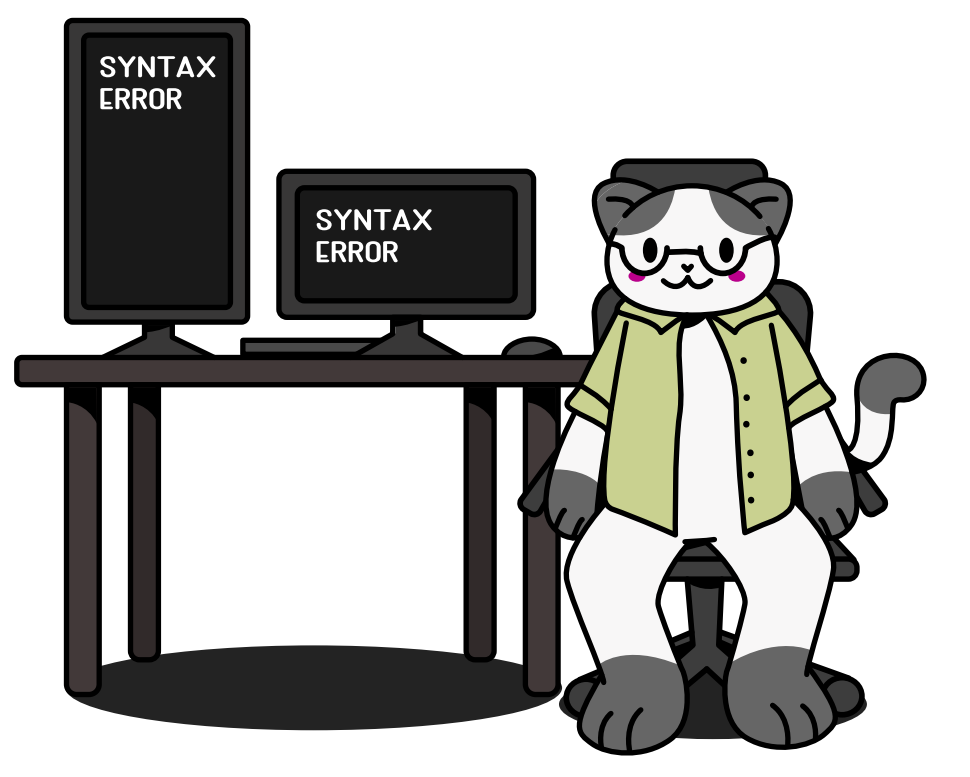
\includegraphics[scale=.38]{assets/03_gatito_sintaxis.PNG}}       
\end{figure}


%Introducción
La sintaxis de un lenguaje de programación permite delimitar el conjunto de las cadenas que pertenecen a este y al mismo tiempo constituye una herramienta de razonamiento para demostrar propiedades utilizando el principio de inducción aplicado a los juicios o reglas que lo definen. \\\\
De forma similar la sintaxis marca la pauta para la definición de funciones como la función de evaluación para obtener el valor asociado a una expresión correctamente construida de un lenguaje de programación y al mismo tiempo será en esta misma estructura donde nos apoyaremos para definir los procesos de análisis para determinar la validez y el tipo de dichas expresiones.\\\\
Para poder comenzar a estudiar los niveles sintácticos de un lenguaje de programación utilizaremos la definición de un nuevo lenguaje el cuál extenderemos con instrucciones a lo largo del desarrollo del manual y lo denominaremos como \textsf{EAB} (expresiones aritmético-booleanas). A partir de la definición de este lenguaje mediante la gramática para generar expresiones y las reglas de inferencia equivalentes abordaremos la construcción y diferencias que existen entre la sintaxis concreta y sintaxis abstracta que se introducen para \textsf{EAB}.\\

\subsection*{Objetivo}
Definir el lenguaje \textsf{EAB} junto con sus diferentes niveles sintácticos, mostrando las principales diferencias que existen entre la sintaxis concreta y abstracta así como estudiar cómo se relacionan proporcionando las reglas para implementar el analizador sintáctico de este mismo.


\subsection*{Planteamiento}
Iniciaremos el estudio de este capítulo brindando las reglas de la sintaxis de \textsf{EAB}\footnote{Este lenguaje es una definición independiente a \textsf{EAL} vista en el \hyperref[sec:intro]{capítulo 1: Introducción}, dado que iremos extendiendo y agregando nuevas instrucciones durante el desarrollo de los siguientes capítulos.} junto con la definición de los nuevos niveles sintácticos; la sintaxis concreta y la sintaxis abstracta, misma que introduce una nueva estructura conocida como árbol de sintaxis abstracta que captura la jerarquía de operación en las instrucciones que se definen en su representación como cadena válida del lenguaje derivada a partir de las reglas definidas en la sintaxis concreta. En particular estudiaremos el proceso mediante el cual una expresión de la sintaxis concreta se relaciona con un árbol de sintaxis abstracta conocido como análisis sintáctico. \\\\
En este nuevo lenguaje vamos a ejemplificar como estos dos niveles sintácticos se relacionan entre sí extendiendo su definición para soportar a los operadores \texttt{if} y \texttt{let}. \\
Posteriormente explicaremos la relación que el operador \texttt{let} introduce con las variables ligadas, variables libres, el alcance de una variable y estudiaremos los conceptos de sustitución y $\alpha$-equivalencia.


%    Section 1: sintaxis concreta y sintaxis abstracta 
\section{Sintaxis concreta}

    La sintaxis concreta se relaciona con la representación gráfica de las cadenas del lenguaje y comúnmente es denotada por una gramática libre de contexto. Esta gramática está pensada para el usuario final, es decir una persona. \\
    A esta capa se le denomina de ''alto nivel'' dado que es un ser humano y no una computadora quien se requiere pueda leer y escribir programas siguiendo las reglas de construcción del lenguaje en cuestión\footnote{Definición formulada a partir de \hyperlink{1}{[1]}, \hyperlink{2}{[2]}, \hyperlink{5}{[5]}, \hyperlink{12}{[12]} y \hyperlink{76}{[76]}}. Vamos a denotar las expresiones del lenguaje con la letra ''\textit{E}''.\\
    Definimos entonces el lenguaje \textsf{EAB}\footnote{Iniciaremos definiendo las instrucciones aritméticas primero y posteriormente agregaremos instrucciones lógico-booleanas con el operador \texttt{if}.} con el siguiente conjunto de juicios: \\
    
    %\begin{definition}
    %    Definición de la grámatica en forma BNF de \textsf{EAB}\footnote{Esta definición fue acuñada a partir de \hyperlink{1}{[1]}, \hyperlink{2}{[2]}, \hyperlink{5}{[5]} y \hyperlink{12}{[12]} adaptada para las instrucciones que nos interesa ejemplificar en este capítulo.}:
    %    \[
    %        \begin{array}{rll}
    %            E & ::= & T \quad |\quad E + T \\
    %            T & ::= & F \quad |\quad T * F \\
    %            F & ::= & N \quad |\quad (E)\\
    %            N & ::= & D \quad |\quad ND \\
    %            D & ::= & 0 \quad |\quad 1 \quad |\quad 2 \quad |\quad 3 \quad |\quad 4 \quad |\quad 5 \quad |\quad 6 \quad |\quad 7 \quad |\quad 8 \quad |\quad 9 
    %        \end{array}
    %    \]
    % \end{definition}

    %De forma equivalente, la gramática previamente mostrada tiene una representación en un conjunto de juicios lógicos.
     
     \begin{definition}
        Sintaxis concreta en forma de juicios lógicos para cada regla en nuestra gramática para \textsf{EAB}\footnote{Esta definición fue acuñada a partir de \hyperlink{1}{[1]}, \hyperlink{2}{[2]}, \hyperlink{5}{[5]} y \hyperlink{12}{[12]} adaptada para las instrucciones que nos interesa ejemplificar en este capítulo.}: 
        \[
            \begin{array}{cccc}
            \inference{}{0\;{\text{D}}}&
            \inference{}{1\;{\text{D}}}&
            \cdots&
            \inference{}{9\;{\text{D}}}
            \end{array}
        \]
        \[
            \begin{array}{cc}
            \inference{d\;{\sf \text{D}}}{d\;{\text{N}}}&
            \inference{n\;{\sf \text{N}}&d\;{\text{D}}}{nd\;{\text{N}}}\\
            &\\
            \inference{n\;{\sf \text{N}}}{n\;{\sf \text{F}}}&
            \inference{e\;{\sf \text{E}}}{(e)\;{\sf \text{F}}}\\
            &\\
            \inference{f\;{\sf \text{F}}}{\text{F}\;{\sf \text{T}}}&
            \inference{t\;{\sf \text{T}}&f\;{\sf \text{F}}}{t*f\;{\sf \text{T}}}\\
            &\\
            \inference{t\;{\sf \text{T}}}{t\;{\sf \text{E}}}&
            \inference{e\;{\sf \text{E}}&t\;{\sf \text{T}}}{e+t\quad{\sf \text{E}}}
            \end{array}
        \]
    \end{definition}

    \section{Sintaxis abstracta}

    La sintaxis abstracta por otra parte como su nombre lo indica se relaciona con la abstracción de la estructura del lenguaje y comúnmente es definida mediante reglas de inferencia para construir un árbol sintáctico donde cada nodo corresponde a una instrucción o operador
     y los hijos a los parámetros que recibe dicha instrucción\footnote{Definición formulada a partir de \hyperlink{5}{[5]}, \hyperlink{12}{[12]}, \hyperlink{77}{[77]}, \hyperlink{78}{[78]} y \hyperlink{79}{[79]}.}. \\\\
    Las hojas de los árboles sintácticos corresponden a los tipos primitivos del lenguaje (enteros, booleanos, caracteres, etc.). En este capítulo vamos a denotar a un árbol de sintaxis abstracta como ''\textit{ASA}''.\\\\
    Los árboles sintácticos son útiles para definir la jerarquía de las operaciones a realizar durante la evaluación de una expresión bien formada de un lenguaje y eliminar la ambigüedad del mismo dado que un árbol de sintaxis abstracta es único sin importar la representación que una expresión tenga en sintaxis concreta. \\\\ 
    %Como mencionamos, existe una representación en sintaxis abstracta para cada expresión bien formada de nuestro lenguaje \textsf{EAB}. Vamos a denotar como ''\textit{ASA}'' a dicha estructura, la cual está definida por el siguiente conjunto de reglas que nos permiten construir el árbol sintáctico correspondiente a dicha expresión. \\

    \begin{definition}
        Sintaxis abstracta de \textsf{EAB}\footnote{Esta definición fue acuñada a partir de \hyperlink{1}{[1]}, \hyperlink{2}{[2]}, \hyperlink{5}{[5]} y \hyperlink{12}{[12]} adaptada para las instrucciones que nos interesa ejemplificar en este capítulo.}
        \[
            \begin{array}{ccc}
                \inference{n\in\N}{num[n]\;\text{ASA}}&
                \inference{t_1\;\textit{ASA}&t_2\;\textit{ASA}}{sum(t_1,t_2)\;\textit{ASA}}&
                \inference{t_1\;\textit{ASA}&t_2\;\textit{ASA}}{prod(t_1,t_2)\;\textit{ASA}}
            \end{array}
        \]
        En donde el predicado $t_1\ ASA$ se lee como: '' $t_1$ es un árbol de sintaxis abstracta''.\\\\
        Es importante notar que los árboles de sintaxis abstracta aunque similares a la expresión en sintaxis concreta que representan corresponden a una categoría distinta de los niveles sintácticos para \textsf{EAB}.
        
    \end{definition}

   \subsection{Analizador sintáctico}
    Al proceso mediante el cual se obtiene el árbol de sintaxis abstracta de una expresión en sintaxis concreta se le conoce como análisis sintáctico. Es importante notar que no siempre será posible encontrar el árbol de sintaxis abstracta (por ejemplo si la expresión que analizamos no es derivable de las reglas de la sintaxis concreta).\\\\
    De tal forma que el objetivo ahora será definir formalmente la relación entre ambos niveles donde el siguiente juicio es válido:\footnote{La definición de esta relación fue formulada a partir de \hyperlink{1}{[1]}, \hyperlink{5}{[5]} y \hyperlink{12}{[12]}, se refiere a las siguientes publicaciones para un estudio en profundidad sobre los niveles sintácticos de los lenguajes de programación: \hyperlink{76}{[76]}, \hyperlink{77}{[77]}, \hyperlink{78}{[78]} y \hyperlink{79}{[79]}}
            \[ e\  E \longleftrightarrow a\ ASA \]
    Esta relación se interpreta como ''a es el árbol de sintaxis abstracta asociado a la expresión e''. Definimos entonces las reglas para implementarla en \textsf{EAB} como sigue:

    \bigskip

    \begin{definition}
        Analizador síntactico para expresiones de lenguaje de EAB\footnote{Definición formulada a partir de \hyperlink{1}{[1]}, \hyperlink{2}{[2]}, \hyperlink{5}{[5]} y \hyperlink{12}{[12]}}
        \[
            \begin{array}{ccc}
                \inference{e\;{\sf N}&e\in\N}{e\;{\sf F}\longleftrightarrow num[e]\;\textit{ASA}}[\textit{(num)}]&
                \quad&
                \inference{e\;{\sf E}\longleftrightarrow a\;\textit{ASA}}{(e)\;{\sf F}\longleftrightarrow a\;\textit{ASA}}[\textit{(parentE)}]\\
                &&\\
                \inference{e\;{\sf F}\longleftrightarrow a\;\textit{ASA}}{e\;{\sf T}\longleftrightarrow a\;\textit{ASA}}[\textit{(fact)}]&
                \quad&
                \inference{e_1\;{\sf T}\longleftrightarrow a_1\;\textit{ASA}&e_2\;{\sf F}\longleftrightarrow a_2\;\textit{ASA}}{e_1*e_2\;{\sf T}\longleftrightarrow prod(a_1,a_2)\;\textit{ASA}}[\textit{(prod)}]\\
                &&\\
                \inference{e\;{\sf T}\longleftrightarrow a\;\textit{ASA}}{e\;{\sf E}\longleftrightarrow a\;\textit{ASA}}[\textit{(exprE)}]&
                \quad&
                \inference{e_1\;{\sf E}\longleftrightarrow a_1\;\textit{ASA}&e_2\;{\sf T}\longleftrightarrow a_2\;\textit{ASA}}{e_1+e_2\;{\sf T}\longleftrightarrow sum(a_1,a_2)\;\textit{ASA}}[\textit{(sum)}]
            \end{array}
        \]
    \end{definition}

    \bigskip
    
    Ahora queremos extender EAB agregando instrucciones booleanas que permitan tener condicionales en nuestras expresiones de lenguaje. Es decir queremos agregar las constantes booleanas \texttt{True} y \texttt{False}, el operador \texttt{if} ... \texttt{then} simple y el operador \texttt{if}... \texttt{then} ... \texttt{else} ... así como parentizado de expresiones para evitar condiciones de ''else colgante''\footnote{Éste problema es conocido en inglés como ''$dangling\ else$'' recurrente en la implementación de \textit{parsers} en el que una cláusula else opcional en una declaración if-then(-else) da como resultado que los condicionales anidados sean ambiguos. \hyperlink{90}{[90]}} y ambigüedad (esta regla puede ser modelada encerrando entre paréntesis la expresión inmediata a evaluar en la instrucción \texttt{then}).

    \bigskip
    
    \begin{exercise}        
        Define la sintaxis concreta para extender nuestro lenguaje \textsf{EAB} con las instrucciones lógicas previamente discutidas\footnote{Definición formulada a partir de \hyperlink{1}{[1]}, \hyperlink{5}{[5]}, \hyperlink{8}{[8]} y \hyperlink{12}{[12]} }
        \[ 
            \inference{}{\texttt{True} \text{ B}} \quad \inference{}{\texttt{False} \text{ B}}
        \]
        \[ 
             \inference{c \text{ B } t \text{ LE }  c \text{ E}}{\texttt{if $c$ then $t$ else $e$ $E$}} \inference{c \text{ B } t \text{ LE}}{\texttt{if $c$ then $t$ E}} \inference{x \text{ B }}{x \text{ LE}}
        \]
        \[
            \inference{e \text{ E}}{(e) \text{ LE}} \inference{e \text{ LE}}{ e \text{ E}}
        \]
    \end{exercise}

    \bigskip

%  Definición alternativa
%        \[ 
%            \inference{\x \in \{a,b\} }{\text{ x Input}}
%            \inference{\x \in \{\top,\bot\} }{\text{ x Output}}
%        \]
%        \[
%            \inference{c \text{ Input } t \text{ ASA  } e \text{ ASA}}{ \textbf{if(} \text{c t e} \textbf{)} \text{ ASA}} 
%            \inference{x \text{ Output }}{ \text{(Out x)} \text{ ASA}}
%        \]
    
    \begin{exercise}
        Define los juicios que componen la sintaxis abstracta para el operador \texttt{If}\footnote{Definición formulada a partir de \hyperlink{1}{[1]}, \hyperlink{5}{[5]}, \hyperlink{8}{[8]} y \hyperlink{12}{[12]} }\\
        \[
            \inference{\texttt{True} \text{ B} }{\textit{T} \textit{ ASA}}
            \inference{\texttt{False} \text{ B} }{\textit{F} \textit{ ASA}}
        \]
        \[
            \inference{c \textit{ ASA } t \textit{ ASA  } e \textit{ ASA}}{ \textit{if} \text{(} \textit{c t e} \text{)} \textit{ ASA}} 
            \inference{c \textit{ ASA } t \text{ ASA  }}{ \textit{if(} \textit{c t} \text{)} \textit{ ASA}} 
        \]
    \end{exercise}

    \bigskip
    
    \begin{exercise}
        Define las reglas del analizador sintáctico para el operador \texttt{If}\footnote{Definición formulada a partir de \hyperlink{1}{[1]}, \hyperlink{5}{[5]}, \hyperlink{8}{[8]} y \hyperlink{12}{[12]} }.
        \[
            \inference{}{\texttt{True} \text{ B} \longleftrightarrow \text{T} \textit{ ASA}}[\textit{(true)}] 
            \inference{}{\texttt{False} \text{ B} \longleftrightarrow \text{F} \textit{ ASA}}[\textit{(false)}]
        \]
        \[
            \inference{\text{$c$ B} \longleftrightarrow \textit{c'}  \textit{ ASA } \quad \text{$t$ LE } \longleftrightarrow \text{$t'$ ASA } \quad \text{$e$ E } \longleftrightarrow \text{e'} \textit{ ASA }}{\texttt{if $c$ then $t$ else $e$ E } \longleftrightarrow \textit{if(c' t' e')} \textit{ ASA} }[$(if_e)$]
        \]
        \[
            \inference{\text{$c$ B} \longleftrightarrow \textit{c'} \textit{ ASA} \quad \text{ $t$ LE} \longleftrightarrow \textit{t' ASA } }
            { \texttt{if($c$ then $t$) E} \longleftrightarrow  \textit{if(c' t')} \textit{ ASA} }[$(if_s)$]
        \]
        \[
            \inference{ \text{$c$ E} \longleftrightarrow \textit{e'} \textit{ ASA}}{\text{($e$) LE} \longleftrightarrow \textit{e'} \textit{ ASA}}[\textit{(parentB)}] \;
            \inference{\text{$c$ B} \longleftrightarrow \textit{c'} \textit{ ASA}}{\text{$c$ LE} \longleftrightarrow \textit{c'} \textit{ ASA}}[\textit{(bool)}] \;
            \inference{\text{$e$ LE} \longleftrightarrow \textit{e'} \textit{ ASA}}{\text{$e$ E} \longleftrightarrow \textit{e'} \textit{ ASA}}[\textit{(exprB)}]
        \]
    \end{exercise}


\section{El operador let}

    Ahora necesitamos extender aún mas \textsf{EAB} para incluir expresiones de tipo: 
    \[\texttt{let } \textit{ x } \text{=} \textit{ $e_1$ } \texttt{in} \textit{ $e_2$ }  \texttt{end}\]

    Donde las apariciones de la variable \textit{x} serán sustituidas por $e_1$ en $e_2$.
    
    Para este propósito se tiene que definir la sintaxis del operador \texttt{let} y el concepto de ligado de variables. \\

    \begin{exercise}
        Proporciona las sintaxis concreta para agregar las instrucciones \texttt{let} de tal forma que sea congruente con las especificación mencionada anteriormente\footnote{Definición formulada a partir de \hyperlink{1}{[1]}, \hyperlink{5}{[5]}, \hyperlink{12}{[12]} y \hyperlink{81}{[81]} }.

        \[
            \inference{e \text{ identificador}}{e\text{ V}}[\textit{(var) }]
            \inference{e\text{ V}}{e\text{ B}}[\textit{(vIn) }]
            \inference{e\text{ V}}{e\text{ F}}[\textit{(vfac) }]
            \inference{x\text{ V} \quad \text{$e_1$ E} \quad \text{$e_2$ E}}{ \texttt{let $x$ = $e_1$ in $e_2$ end E}}[\textit{(let)}]
        \]
    \end{exercise}


    La sintaxis abstracta de orden superior define un tratamiento especial para las variables que se introducen con el operador \texttt{let} así como el alcance y ligado de las mismas. Esta sintaxis abstrae estos niveles como parte del metalenguaje con el que se define el árbol de sintaxis abstracta, es decir vamos a delimitar el rango de aplicación de la variable con el árbol que definiremos para el operador mismo.\\\\
    Extenderemos nuestro lenguaje \textsf{EAB} agregando el árbol de sintaxis abstracta \textit{x.t} que indica que la variable \textit{x} está ligada
    en el árbol \textit{t}, a este \textit{ASA} se le llama abstracción\footnote{Definición acuñada a partir de \hyperlink{1}{[1]}, \hyperlink{2}{[2]}, \hyperlink{5}{[5]}, \hyperlink{12}{[12]}, \hyperlink{80}{[80]} y \hyperlink{81}{[81]}}. Esto es importante dado que al introducir las variables ligadas y su alcance tenemos que delimitar la expresión en la que la sustitución ocurrirá.

    \begin{exercise}
        Proporciona las sintaxis Abstracta para agregar las instrucción \texttt{let}\footnote{Definición formulada a partir de \hyperlink{1}{[1]}, \hyperlink{5}{[5]}, \hyperlink{12}{[12]} y \hyperlink{81}{[81]} } considerando el \textit{ASA} \textit{x.t}.
        \[
            \inference{\text{$x$ identificador}}{\text{var[$x$] \textit{ASA}}}[] 
            \inference{\textit{$a_1$ \textit{ASA}} \quad \textit{$a_2$ \textit{ASA}} }{\text{\textit{let(}$a_1$, $x$.$a_2$\textit{)} \textit{ASA}}}[]
        \]
    \end{exercise}

    \bigskip

    \begin{exercise}
         Define las reglas del analizador sintáctico para agregar las instrucción \texttt{let}\footnote{Definición formulada a partir de \hyperlink{1}{[1]}, \hyperlink{5}{[5]}, \hyperlink{12}{[12]} y \hyperlink{81}{[81]} }.
         \[
            \inference{x \text{ identificador}}{\text{$x$ V} \longleftrightarrow \text{var[$x$] \textit{ASA}}}[\textit{ vara }]
            \inference{\text{$x$ V} \quad \text{$e_1$ E} \longleftrightarrow \textit{$a_1$ ASA} \quad \text{$e_2$ E} \longleftrightarrow \text{$a_2$ \textit{ASA}} }
                      {\texttt{let $x$ = $e_1$ in $e_2$ end E} \longleftrightarrow \textit{let($a_1$ $x$.$a_2$) \textit{ASA}}}[\textit{leta}]
         \]
    \end{exercise}

    \bigskip

    A continuación tenemos tres ejemplos que nos van a ayudar a ilustrar la aplicación de las reglas que hemos definido hasta el momento para construir los \textit{ASA} de \textsf{EAB} partiendo de expresiones derivadas de las reglas de la sintaxis concreta.

    \bigskip

    \begin{exercise}
        Obtén la representación en sintaxis abstracta partiendo de la sintaxis concreta de las siguiente expresión: \\\\
        \texttt{let} $x$ = 1 \texttt{in} $x$ + 1 \texttt{end}\\
        \[
            \textit{let(num[1], $x.$var[$x$]+1)}\ ASA
        \]
    \end{exercise}

    \begin{exercise}
        Obtén la representación en sintaxis abstracta partiendo de la sintaxis concreta de las siguiente expresión: \\\\
        \texttt{let} $y$ = \texttt{if} \texttt{True} \texttt{then} 1 \texttt{else} 0 \texttt{in} \texttt{if} $x$ \texttt{then} \texttt{False} \texttt{end}\\
        \[
            \textit{let(if(T, num[1], num[0]), $y$.if(var[$x$], F))\ ASA}
        \]
    \end{exercise}

    \begin{exercise}
        Obtén la representación en sintaxis abstracta partiendo de la sintaxis concreta de las siguiente expresión: \\
        
        \texttt{let $x$ = False} \texttt{in} \texttt{if} $x$ \texttt{then} (\texttt{if} $\alpha$ \texttt{then} (\texttt{if} $\alpha$ \texttt{then} 4)) \texttt{else False} \texttt{end}\\
        \[
            \textit{let(F, x.if(var[x], if(var[$\alpha$], if(var[$\alpha$], num[4])), F)) ASA}
        \]        
    \end{exercise}

    \bigskip

    \subsection{Clasificación de variables en el operador let}
    
    La introducción de nuestro nuevo operador \texttt{let} acarrea consigo la definición de ligado de una variable, variable ligada\footnote{Aún que los nombres son similares ligado de una variable y variable ligada corresponden a dos definiciones distintas.}, variable libre y la definición de la función de sustitución junto con la función para obtener variables libres de una expresión, mismas que serán mostradas a continuación y serán de utilidad para resolver el resto de los ejercicios presentes en este capítulo.\\
    
    \begin{definition}Ligado de una variable: la instancia de ligado de una variable es aquella que da a esta su valor\footnote{Definición formulada de \hyperlink{2}{[2]}, \hyperlink{5}{[5]}, \hyperlink{12}{[12]}, \hyperlink{80}{[80]} y \hyperlink{81}{[81]}}. Es decir, es la aparición de la variable en donde esta es definida. \\\\
    De tal forma que si tenemos la siguiente expresión: \[ \texttt{let } x = e_1 \texttt{ in } e_2 \texttt{ end } \] Decimos que $x = e_1$ es el ligado de la variable \textit{x} en la instrucción \texttt{let}.
    \end{definition}

    \bigskip

    \begin{definition}Variable ligada: sea \textit{x.t} un \textit{ASA}, decimos que \textit{x} está ligada en \textit{t} para todas las apariciones de \textit{x}\footnote{Definición formulada de \hyperlink{2}{[2]}, \hyperlink{5}{[5]}, \hyperlink{12}{[12]}, \hyperlink{80}{[80]} y \hyperlink{81}{[81]}}.\\\\
    De tal forma que si tenemos la siguiente expresión: \[ \texttt{let } x = e_1 \texttt{ in } e_2 \texttt{ end } \] Decimos que $x $ es la variable ligada en $e_2$ dentro de nuestra expresión \texttt{let}.
    \end{definition}

    \bigskip

    \begin{definition}Variable libre: una variable está libre en una expresión, si no se encuentra dentro del alcance de una variable de ligado con su nombre. Es decir, una variable es libre si no está ligada\footnote{Definición formulada de  \hyperlink{2}{[2]}, \hyperlink{5}{[5]}, \hyperlink{12}{[12]}, \hyperlink{80}{[80]} y \hyperlink{81}{[81]}}.\\\\
    De tal forma que si tenemos la siguiente expresión: \[ \texttt{let } x = e_1 \texttt{ in } y \texttt{ end } \] Decimos que $y$ es una variable libre en nuestra expresión \texttt{let}.
    \end{definition}

    \bigskip
    
    \begin{definition}Función para obtener las variables libres de una expresión: dado el árbol de sintaxis abstracta $a$  definimos el conjunto de variables libres de la expresión\footnote{Definición extraída de  \hyperlink{2}{[2]}, \hyperlink{5}{[5]}, \hyperlink{12}{[12]}, \hyperlink{80}{[80]} y \hyperlink{81}{[81]}}, denotado $FV(a)$ como sigue:
        \[
            \begin{array}{lcl}
                FV(x)&=&\{x\}\\
                FV(O(a_1,\cdots,a_n))&=&FV(a_1)\cup\cdots\cup FV(a_n)\\
                FV(x.a)&=&FV(a)\backslash\{x\}
            \end{array}
        \]
    \end{definition}

    \bigskip

    \begin{exercise}
    Dada la siguiente expresión \texttt{let} definida como:
    \begin{align*}
    	e=_{\text{def}}\texttt{let  }
    		x&= \texttt{let }x = (2 + 4) \texttt{ in } x+1 \texttt{ end }
    		\texttt{ in }\\
    		 &\texttt{let }y=(x \ast 2)+x 
    		 	\texttt{ in } \\
    		 & \qquad(x\ast y) + \texttt{let }z=7 \texttt{ in } 
    		 						y+z 
    		 				\texttt{ end }\\
    		 &\texttt{ end }\\
    	\texttt{ end }&
    \end{align*}

    Por cada subexpresión \textsf{let} en $e$ (inclusive) proporciona el alcance indicado o subrayando las variables ligadas.

    
    \begin{align*}
    	e=_{\text{def}}\texttt{let  }
    		\setulcolor{blue}\textit{\ul{x}}&= \texttt{let }\setulcolor{purple}\textit{\ul{x}} = (2 + 4) \texttt{ in } \setulcolor{purple}\textit{\ul{x}}+1 \texttt{ end }
    		\texttt{ in }\\
    		 &\texttt{let }\setulcolor{green}\textit{\ul{y}} =( \setulcolor{blue}\textit{\ul{x}} \ast 2)+ \setulcolor{blue}\textit{\ul{x}} 
    		 	\texttt{ in } \\
    		 & \qquad( \setulcolor{blue}\textit{\ul{x}}\ast \setulcolor{green}\textit{\ul{y}}) + \texttt{let }\setulcolor{orange}\textit{\ul{z}}=7 \texttt{ in } 
    		 						\setulcolor{green}\textit{\ul{y}}+\setulcolor{orange}\textit{\ul{z}}
    		 				\texttt{ end }\\
    		 &\texttt{ end }\\
    	\texttt{ end }&
    \end{align*}
    
    \end{exercise}

    \bigskip

    \begin{exercise}
    Escribe cada subexpresión let en $e$ (inclusive) indicando la variable de ligado y la expresión \texttt{let} para la cual la variable de ligado tiene alcance.
    
        \begin{align*}
    	\texttt{let  }
    		\setulcolor{blue}\textit{\ul{x}}&= \texttt{let }x = (2 + 4) \texttt{ in } x+1 \texttt{ end }
    		\texttt{ in }\\
    		 &\texttt{let }y=(x \ast 2)+x 
    		 	\texttt{ in } \\
    		 & \qquad(x\ast y) + \texttt{let }z=7 \texttt{ in } 
    		 						y+z 
    		 				\texttt{ end }\\
    		 &\texttt{ end }\\
    	\texttt{ end }&
        \end{align*}

        La siguiente expresión \texttt{let} es la que le da su valor a la variable más externa definida en $e$ la cual se identifica como: 
        \begin{align*}
    		\texttt{let }\setulcolor{purple}\texttt{\ul{x}} = (2 + 4) \texttt{ in } x+1 \texttt{ end }
        \end{align*}

        La expresión \texttt{let} que continua está delimitada por los marcadores más externos \texttt{in} \texttt{end} en $e$ y se identifica como: 
        \begin{align*}
    	   &\texttt{let }\setulcolor{green}\texttt{\ul{y}}=(x \ast 2)+x  \texttt{ in } \\	 
                        &\qquad(x\ast y) + \texttt{let }z=7 \texttt{ in } y+z \texttt{ end }\\
    		 &\texttt{ end }\\
        \end{align*}

        La útltima expresión \texttt{let} está delimitada por los marcadores \texttt{in} \texttt{end} de la expresión anterior y se identifica como: 
        \begin{align*}
                 &\texttt{let } \setulcolor{orange}\texttt{\ul{z}}=7 \texttt{ in } y+z \texttt{ end }\\
        \end{align*}
    \end{exercise}

    \bigskip

    \begin{exercise}
        La expresión $e$ se puede evaluar a un valor? si sí muestra el procedimiento para la evaluación informal (aún no definimos la manera en la que se va a evaluar la expresiones del lenguaje \textsf{EAB} pero se puede dar una idea de la evaluación partiendo de la descripción hecha en el capítulo).
    
        \begin{align*}
        	e=_{\text{def}}\texttt{let  }
        		x&= \texttt{let }x = (2 + 4) \texttt{ in } x+1 \texttt{ end }
        		\texttt{ in }\\
        		 &\texttt{let }y=(x \ast 2)+x 
        		 	\texttt{ in } \\
        		 & \qquad(x\ast y) + \texttt{let }z=7 \texttt{ in } 
        		 						y+z 
        		 				\texttt{ end }\\
        		 &\texttt{ end }\\
        	\texttt{ end }&
        \end{align*}
    
        Primero se resuelve la expresión let que la da valor a la variable $x$ en la expresión $e$:
        \[
            \texttt{let }x = (2 + 4) \texttt{ in } x+1 \texttt{ end } 
             = (2+4) + 1 
             = (6) + 1
             = 7
        \]
        Se sustituye este valor en el cuerpo de $e$ resultando en la siguiente expresión:
        \begin{align*}
            &\texttt{let }y =(7 \ast 2)+7  \texttt{ in }\newline
            &\qquad(7\ast y) + \texttt{let }z=7 \texttt{ in } y+z \texttt{ end }\newline
            &\texttt{ end }
        \end{align*}
        Resolviendo la operación para dar variable a la variable y obtenemos el siguiente resultado: 
        \[
            y = (7 \ast 2) + 7 
            = (14) + 7 
            = 21
        \]
        Sustituyendo el nuevo valor en el cuerpo de la expresión anterior se obtiene:
        \begin{align*}
                 & = (7 \ast 21) + \texttt{let } z=7 \texttt{ in } 21 + z \texttt{ end }
        \end{align*}
        Resolviendo las operaciones y la sustitución de la variable $z$ en el cuerpo de la expresión let se obtiene:
        \[
            = 147 + 21 + 7
            = 168 + 7
            = 175
        \]

    \end{exercise}

    \bigskip
    
    \begin{exercise}
        En nuestra expresión $e$ hay variables libres, argumenta por qué si o por qué no. \\
    
        No, todas las variables definidas en la expresión $e$ están asociadas a un operador \texttt{let} marcando su alcance en las expresiones anidadas presentes por lo que ninguna variable aparece sin su respectiva asociación.
    \end{exercise}


\section{Sustitución y $\alpha$-equivalencias}
    Para finalizar este capítulo se introduce el concepto de alfa equivalencia:

    \begin{definition}$\alpha$-equivalencia: se dice que dos expresiones $e_1$ y $e_2$ son $\alpha$-equivalentes si y sólo si difieren únicamente en el nombre de las variables ligadas\footnote{La notación de la relación de $\alpha$-equivalencia fue extraída de \hyperlink{1}{[1]}, \hyperlink{5}{[5]} y \hyperlink{12}{[12]}, la definición formulada a partir de \hyperlink{81}{[81]} y \hyperlink{89}{[89]}}.\\\\
    Esta relación será denotada como: 
    \begin{center}
            $e_1\equiv_\alpha e_2$        
    \end{center}
    \end{definition}

    Esta definición resulta de utilidad para trabajar con expresiones que necesiten ser renombradas a lo más en sus variables ligadas para poder aplicar la sustitución sobre dicha expresión cuando haya un conflicto ocasionado por los identificadores. \\\\
    A continuación definimos la función de sustitución aplicada a expresiones pertenecientes a nuestro lenguaje \textsf{EAB}.

    
    \begin{definition}Función de sustitución: se define la función de sustitución\footnote{Esta definición está formulada a partir de \hyperlink{1}{[1]}, \hyperlink{2}{[2]}, \hyperlink{5}{[5]} y \hyperlink{12}{[12]} adaptada para las instrucciones que hemos revisado hasta este momento para \textsf{EAB}.} sobre los árboles de sintaxis abstracta de \textsf{EAB}:
        \[
            \begin{array}{lclr}
                var[x][var[x]:=e]&=&e&\\
                var[z][var[z]:=e]&=&var[z]&\\
	     T\; [var[z]:=e]& =& T \\
	     F\; [var[z]:=e] &=& F\\
                num[n][var[x]:=e]&=&num[n]&\\
                sum(a_1,a_2)[var[x]:=e]&=&sum(a_1[var[x]:=e],a_2[var[x]:=e])&\\
                prod(a_1,a_2)[var[x]:=e]&=&prod(a_1[var[x]:=e],a_2[var[x]:=e])&\\
                let(a_1,a_2)[var[x]:=e]&=&let(a_1[var[x]:=e],a_2[var[x]:=e])&\\
                if(a_1,a_2)[var[x]:=e]&=&if(a_1[var[x]:=e],a_2[var[x]:=e])&\\
                if(a_1,a_2,a_3)[var[x]:=e]&=&if(a_1[var[$x$]:=e],a_2[var[x]:=e],a_3[var[x]:=e])&\\
                (z.a)[var[x]:=e]&=&z.(a[var[x]:=e]) \; \mbox{Si }x\neq z\mbox{ y }z\not\in FV(e)\\
                (z.a)[var[x]:=e]&=&{\tt indefinido} \; \mbox{Si }z\in FV(e)\\
            \end{array}
        \]
    \end{definition} 

    \bigskip

    \begin{exercise}
        Proporciona una expresión $\alpha$-equivalente a la siguiente expresión:\\
        $\texttt{let } x = \texttt{ let } y = \texttt{ False } \texttt{ in } \texttt{\texttt{ if } (y \texttt{then} 1 \texttt{else} 0)} \texttt{ in } (x + 2) * w \texttt{ end}$ 
        \[
            \texttt{let } k = \texttt{ let } j = \texttt{ False } \texttt{ in } \texttt{\texttt{ if } (j \texttt{then} 1 \texttt{else} 0)} \texttt{ in } (k + 2) * w \texttt{ end} 
        \]
    \end{exercise}

    \bigskip

    \begin{exercise}
        Proporciona una expresión $\alpha$-equivalente a la expresión $e$ definida en el ejercicio 3.7.
        \begin{align*}
        	e_\alpha = \texttt{let  }
        		a&= \texttt{let }d = (2 + 4) \texttt{ in } d+1 \texttt{ end }
        		\texttt{ in }\\
        		 &\texttt{let }b=(a \ast 2)+a 
        		 	\texttt{ in } \\
        		 & \qquad(a\ast b) + \texttt{let }c=7 \texttt{ in } 
        		 						b+c 
        		 				\texttt{ end }\\
        		 &\texttt{ end }\\
        	\texttt{ end }&
        \end{align*}
    \end{exercise}

    \begin{exercise}
        Desarrolla la sustitución aplicada a la siguiente expresión de acuerdo con la función de sustitución previamente definida.
        \[
            \texttt{let } x = (w + 1) * 2 \texttt{ in} \texttt{ if (} \texttt{True } \texttt{ then } w \texttt{ else } (2 * x) \texttt{)} \texttt{ end }[w:=2]
        \]
        \[
            = \textit{let(prod(sum(var[w], 1), 2), if(T, var[w], prod(2, var[x])))\; [var[w] := 2]}
        \]
        \[
            \scalemath{0.81}{
             =  \textit{let(prod(sum(var[w], 1), 2) \; [var[w] := 2], if(T, var[w], prod(2, var[x]))\; [var[w] := 2] )}
            }
        \]
        \[
            \scalemath{0.6}{
               =  \textit{let(prod(sum(var[w], 1) [var[w] := 2], 2 [var[w] := 2]), if(T [var[w] := 2], var[w] [var[w] := 2], prod(2, var[x])[var[w] := 2] ))}
            }
        \]
        \[
	\scalemath{0.7}{
             =  \textit{let(prod(sum(var[w] [var[w] := 2] , 1[var[w] := 2]), 2), if(T, 2, prod(2 [var[w] := 2], var[x] [var[w] := 2])))}
 	}
        \]
        \[
	\scalemath{1}{
             =  \textit{let(prod(sum(2, 1), 2), if(T, 2, prod(2, var[x])))}
 	}
        \]

    \end{exercise}

    
\section{Ejercicios para el lector}

    \begin{exercise}
        Explica con tus palabras la diferencia entre la sintaxis abstracta y la sintaxis concreta.
    \end{exercise}

    \bigskip

    \begin{exercise}
        Explica con tus palabras por que es necesaria la sintaxis abstracta de orden superior que se introduce con el árbol de sintáxis abstracta \textit{x.t}
    \end{exercise}

    \bigskip

    \begin{exercise}
        Proporciona el árbol de sintaxis abstracta para la siguiente expresión \texttt{let}
        \[ 
            \texttt{let } z = 777 \texttt{ in } (w + h) * (z) + \texttt{ let } v = -33 \texttt{ in } (z * z) + v \texttt{ end } \texttt{ end } 
        \]
    \end{exercise}

    \bigskip
    
    \begin{exercise}
        Proporciona el árbol de sintaxis abstracta para la siguiente expresión \texttt{if}
        \[
            \texttt{if(} \texttt{True} \texttt{ then } \texttt{if(}  \texttt{False} \texttt{ then } 0) \texttt{ else } (2 * 7) - 1 \texttt{)}
        \]
    \end{exercise}

    \bigskip
    
    \begin{exercise}
        La siguiente expresión ¿es una expresión correcta de nuestro lenguaje? Explica por que si o porque no de acuerdo a las reglas de sintaxis concreta definidas.
        \[
            \texttt{if(} \top \texttt{ then } \texttt{ let } x = True \texttt{ in } \texttt{ if (} x \texttt{ then } \bot \texttt{)} \texttt{ end} \text{)}
        \]
    \end{exercise}

    \bigskip
    
    \begin{exercise}
        Dada la siguiente expresión let definida como:
        \begin{align*}
        	e_1=_{\text{def}}\texttt{let  }
        		x&= \texttt{let }x = 2 \texttt{ in } \texttt{ let } y = 3 \texttt{ in } y + x \texttt{ end } \texttt{ end }
        		\texttt{ in }\\
        		 &\texttt{let }y=(x \ast 2) \ast 19 
        		 	\texttt{ in } \\
        		 & \qquad(x + y) \ast \texttt{let } z = \texttt{ let } v = 8 \texttt{ in } z \texttt{ end } \texttt{ in } 
        		 						(y + z) \ast v 
        		 				\texttt{ end }\\
        		 &\texttt{ end }\\
        	\texttt{ end }&
        \end{align*}
        Proporciona lo siguiente por cada subexpresión \texttt{let} definida en $e$:
        \begin{itemize}
            \item Las variables ligadas
            \item Las variables libres
            \item El alcance de cada variable
            \item El valor que se obtiene al desarrollar la expresión.
        \end{itemize}
    \end{exercise}

    \bigskip
    
    \begin{exercise}
        Proporciona una expresión $\alpha$-equivalente a $e_1$ del ejercicio anterior 
    \end{exercise}

    \bigskip
    
    
    \begin{exercise}
         Desarrolla la siguiente sustitución, en caso de ser inválida explica por qué.
         \[
         \texttt{ let } z = 3 \texttt{ in } (w + z) + \texttt{ if(} \texttt{True} \texttt{ then } 45 \texttt{ else } y \texttt{) } \texttt{end } [y:=7]
         \]
    \end{exercise}

    \bigskip
    
    \begin{exercise}
        Desarrolla la siguiente sustitución paso por paso, en caso de ser inválida explica por qué. 
        \[
            \texttt{ let } z = 3 \texttt{ in } (w + z) + \texttt{ if (} \texttt{True} \texttt{ then } 45 \texttt{ else } y \texttt{)} \texttt{ end } [y:=z+7]
        \]
    \end{exercise}

    \bigskip

   \begin{exercise}
        A continuación se define la sintaxis concreta para un lenguaje funcional simple:
        \[ e ::=  \text{ $x$ } \text{$|$} \text{ $n$  }\text{$|$} \text{ } e_1 \text{ } e_2 \text{ } \text{$|$} \text{ } fun(x) \rightarrow e \]

    En donde el primer constructor representa las variables del lenguaje, el segundo números naturales,
    el tercero aplicación de función y el último la definición de funciones.\\

    De acuerdo a la especificación discutida anteriormente, contesta los siguiente incisos: \\
    \begin{itemize}
        \item Define las reglas de inferencia para la sintaxis concreta de la gramática anterior.
        \item Diseña una sintaxis abstracta apropiada para este lenguaje (Primero observa si es necesario alguna especie de ligado como el que define el operado \texttt{let} discutido en este capítulo).
        \item Escribe las reglas para la relación de análisis sintáctico ($\longleftrightarrow$) del lenguaje.
        \item Diseña un algoritmo de sustitución para este lenguaje.
        \item La relación de $\alpha$-equivalencia en este lenguaje se da respecto al operador de definición de función $fun$. Se dice que dos expresiones son $\alpha$-equivalentes si solo difieren en el nombre de la variable del parámetro de la función. Por ejemplo:
              \[ fun(x) \rightarrow e \equiv_\alpha fun(y) \rightarrow e \]
              Demuestra que $\equiv_\alpha$ es una relación de equivalencia.
    \end{itemize}

   \end{exercise}
    
		
		\chapter{Semántica}
		\label{sec:semantics}
			%    Cuarto Capítulo capítulo: Siintáxis.
%    Ejercicios por Barón L. Miguel.
%    Teoría por Javier Enríquez Mendoza.
%    Empezado el 29/11/22
%    Concluido el 17/1/23

%Gatito Sintáctico
\begin{figure}[htbp]
    \centerline{
\includegraphics[scale=.4]{assets/04_gatito_semantica.jpg}}       
\end{figure}


%Introducción
\bigskip
\bigskip
\bigskip
\bigskip


    En el capítulo anterior se estudió la composición sintáctica de las expresiones de nuestro lenguaje mediante juicios que nos permiten construir una instrucción utilizando la sintaxis
    concreta y el árbol de sintaxis abstracta asociado a la misma. Estos niveles sintácticos nos permiten responder a la pregunta ¿qué es una expresión de lenguaje?.\\\\
    En el presente capítulo nos ocuparemos de la semántica del lenguaje, que tiene como propósito responder a la pregunta ¿qué significa una expresión del lenguaje?.\\
    En el contexto de los lenguajes de programación podemos pensar de forma intuitiva que la respuesta a la pregunta anterior sería algo como: ''el comportamiento que tiene la expresión del lenguaje en tiempo de ejecución al ser evaluada''. 
    En particular  nos interesa obtener el valor al que la expresión del lenguaje se evalúa (semántica dinámica) y analizar el tipo de la expresión (semántica estática)\footnote{Definición acuñada de \hyperlink{98}{[98]}, \hyperlink{99}{[99]} y \hyperlink{100}{[100]}}.\\\\
    Muchas veces en la documentación oficial de los lenguajes de programación la semántica está escrita en un manual el cual contiene una descripción de alto nivel
    acerca de como una determinada instrucción, método o expresión se comporta al momento de ejecutarse. Si bien esto resulta útil al escribir un programa nuestro interés sera definir formalmente la semántica de ejecución mediante juicios y reglas para el lenguaje \textsf{EAB}. \\

    \subsection*{Objetivo}
        Definir los diferentes niveles semánticos de \textsf{EAB} mediante reglas de inferencia que dictaminen el proceso que se 
        debe seguir al para evaluar o asignar un tipo a una expresión bien formada de este lenguaje.

    \subsection*{Planteamiento}
        Iniciaremos el estudio de este capítulo presentando las reglas para poder asignar un tipo a cada un de las expresiones bien formadas de \textsf{EAB}. Este nivel corresponde a la semántica estática y será de utilidad para fundamentar la seguridad del lenguaje y garantizar que se pueda regresar un valor al final de la evaluación de la expresión a la que se pretende asignar el tipo.\\\\
        Posteriormente se definirá el procedimiento para evaluar las expresiones bien formadas de \textsf{EAB}. Este mecanismo se conoce como semántica dinámica y se estudiará en dos paradigmas: de paso grande y de paso pequeño. Por último definiremos la función \texttt{eval} para \textsf{EAB}.

    \section{Semántica estática}
    La semántica estática extrae información del programa en tiempo de compilación, la cantidad y calidad de la información obtenida depende de la implementación de cada compilador\footnote{Definición acuñada de \hyperlink{96}{[96]} y \hyperlink{97}{[97]}}. \\\\
    La información que se extrae del programa provisto por el usuario puede ser: el alcance de una variable, el tipo de una expresión, saber si una expresión tiene variables libres, etc. Saber esto es indispensable  para poder evaluar las expresiones de \textsf{EAB} (este último punto es importante ya que necesitamos que todas las variables estén ligadas y no haya presencias libres en nuestras expresiones, de lo contrario de la evaluación no se obtendrá valor alguno).\\\\
    En el lenguaje de expresiones aritméticas con el que hemos estado trabajando, las expresiones de la forma:
        \begin{center}
                \texttt{let}\ \textit{x}\ =\ \textit{y}\ \texttt{in}\ \textit{x}\ +\ \textit{x}\ \texttt{end}
        \end{center}
    son sintácticamente correctas pero semánticamente incorrectas, pues la variable \textit{y} está libre en la expresión por lo que no podría evaluarse.\\\\
    Ésta es una de las propiedades de las que se encarga la semántica estática, así que daremos un conjunto de reglas para definir una semántica estática encargada de evitar estos errores. Para esto se define el siguiente juicio: 

    \bigskip
    
    \begin{definition}Semántica estática para capturar expresiones con variables libres en \textsf{EAB}\footnote{Definición acuñada de \hyperlink{2}{[2]}, \hyperlink{5}{[5]} y  \hyperlink{12}{[12]} }:
    Sea $\Delta$ un conjunto de variables y \textit{a} un árbol de sintáxis abstracta, decimos que \textit{a} no tiene variables libres en bajo el conjunto $\Delta$ denotado como:
        $$ \Delta\sim a\ ASA$$
    
    En particular nos interesa que todas las variables ligadas de \textit{a} estén presentes en $\Delta$.\\
    Para construir este conjunto definimos las siguientes reglas que nos permitirán acrecentar $\Delta$ cada que encontremos una variable ligada en el árbol $x.t$. Definimos las reglas como sigue:
    \[
        \begin{array}{ccc}
            \inference{x\in \Delta}{\Delta \sim\ x}[\textsf{fvv}]&
            \inference{}{\Delta \sim num[n]}[\textsf{fvn}]&
            \inference{\Delta, x \sim e}{\Delta \sim\ x.e}[\textsf{fva}]
        \end{array}
    \]
    \bigskip
    \[
        \begin{array}{cc}
            \inference{}{\Delta\sim \textit{T}\ \text{ Bool}}[{\sf fvb}]&
            \inference{\Delta\sim e_1&\cdots&\Delta\sim e_n}{\Delta\sim O(e_1,\cdots,e_n)}[{\sf fvo}]
        \end{array}
    \]

    \bigskip
    
    Para garantizar que una expresión $e$ no tiene variables libres se inicia con el conjunto vacío y se debe probar $\emptyset\sim e$ usando las reglas anteriores.
    \end{definition}

    \bigskip

    \begin{definition}Expresión cerrada de \textsf{EAB}\footnote{Definición acuñada de \hyperlink{2}{[2]}, \hyperlink{5}{[5]} y  \hyperlink{12}{[12]}}:
    Sea $a$ un \textit{ASA} decimos que $a$ es cerrada si y sólo si $$ FV(a)\ =\ \emptyset $$
    Es decir, $a$ es una expresión del lenguaje cerrada si no tiene apariciones de variables libres. 
    \end{definition}

    \bigskip

    \begin{exercise}
        Para la siguiente expresión realiza el análisis estático para encontrar variables libres mediante la derivación aplicando las reglas del juicio $\sim$
        \[ 
            \texttt{let } x = 1 \texttt{ in } (y * x) + z \texttt{ end}
        \]
        \[
            \inference{\inference{\inference{\inference{\texttt{Error}}{\{ x \} \sim y} & \inference{x \in \{x\}}{\{ x \} \sim x}[(fvn)]}{\{ x \} \sim (y * x)}[(fvo)] & \inference{Error}{\{ x \} \sim z} }{\{ x \} \sim \text{(y * x) + z}}[(fvo)]}{\emptyset \sim \texttt{let } x = 1 \texttt{ in } \text{($y$ * $x$) + $z$} \texttt{ end}}[(fva)]
        \]
    \end{exercise}

    \bigskip

    \begin{exercise}
        Para la siguiente expresión realiza el análisis estático para encontrar variables libres mediante la derivación aplicando las reglas del juicio $\sim$
 
            \[
                 \texttt{ if  } \texttt{True } \texttt{then } (1 + 1) * 2  \texttt{ else } 7 
            \]
            \[
	\scalemath{0.7}{
                \inference{\inference{}{\emptyset \sim True}[(fvb)] & \inference{\inference{\inference{}{\emptyset \sim 1}[(fvn)] & \inference{}{\emptyset \sim 1}[(fvn)]}{\emptyset \sim (1 + 1)}[(fvo)] & \inference{}{\emptyset \sim 2}[(fvn)]}{\emptyset \sim (1 + 1) * 2}[(fvo)] & \inference{}{\emptyset \sim 7}[(fvn)] }{\emptyset \sim \textbf{ if } True \textbf{ then } (1 + 1) * 2 \textbf{ else } 7  }[fvo]
	}           
 \]


    \end{exercise}

    \bigskip

    \begin{exercise}
        Para la siguiente expresión realiza el análisis estático para encontrar variables libres mediante la derivación aplicando las reglas del juicio $\sim$
        \[
            1 + \texttt{if ( } \texttt{ let } x = \texttt{True} \texttt{ in } x \texttt{ end } \texttt{ then } 2 \texttt{ else } 1 \texttt{ )}
        \]
        \[
\scalemath{0.8}{
            \inference{\inference{}{\Delta \sim 1}[(fvn)] \inference{ \inference{\inference{}{\{x\} \sim x}[(fvn)]}{\Delta \sim \texttt{ let } x = \texttt{True} \texttt{ in } x \texttt{ end }}[(fvo)] \inference{}{\Delta \sim 2}[(fvn)] \inference{}{\Delta \sim 1}[(fvn)] }{\Delta \sim \texttt{if ( } \texttt{ let } x = \texttt{True} \texttt{ in } x \texttt{ end } \texttt{ then } 2 \texttt{ else } 1 \texttt{ )}}[(fvo)]}{\Delta \sim 1 + \texttt{if ( } \texttt{ let } x = \texttt{True} \texttt{ in } x \texttt{ end } \texttt{ then } 2 \texttt{ else } 1 \texttt{ )}}[(fvo)]
}
        \]
    \end{exercise}

    \bigskip

    De los ejercicios anteriores podemos notar que el análisis sintáctico para evaluar  expresiones con variables libres fallará en una o más ramas, mientras que los árboles de derivación generados de expresiones cerradas concluirán todas sus ramas con algún axioma (fvn, fvb  o fvv). \\\\

    \section{Semántica dinámica}
    La semántica dinámica constituye el siguiente eslabón del proceso de ejecución de un programa. Una vez verificada que la expresión en sintáxis concreta es una expresión válida y no posee variables libres por la semántica estática, entonces se puede comenzar a discutir el cómo se ejecutará dicha expresión. \\\\\
    Diferentes paradigmas de ejecución pueden ser aplicados para las expresiones de \textsf{EAB} dependiendo de la rama de interés que se quiera estudiar del lenguaje de programación (por ejemplo cambios en la memoria, el valor las variables del programa, el valor final al que reduce la expresion, etc). En este capítulo nos centraremos en la semántica operacional que estudia el proceso de ejecución modelando cada configuración del programa como un estado y las transiciones entre ellos.
    
    
    \subsection{Semántica operacional}
    En esta categoría se hace la distinción entre los dos paradigmas mas imprtanes para estudiar la semántica operacional de los lenguajes de programación:
    \begin{itemize}
        \item Semántica de paso pequeño: la cuál modela la ejecución de un programa describiendo las transiciones una a una mostrando los compútos generados de forma individual. 
        \item Semántica de paso grande: que contrasta con la de paso pequeño porque aquí no nos importa que estados sucedieron en la ejecución del programa, únicamente nos interesa el valor que regresa.
    \end{itemize}

   % Como ambos enfoques solo difieren en el sistema de transición que emplean definiremos los estados de la máquina de transición para ambos a continuación.

    \bigskip
    
    \begin{definition}Sistema de transición para la semántica operacional de \textsf{EAB}:  Se define la semántica operacional del lenguaje de expresiones aritméticas utilizando el sistema de transición siguiente:
    \vspace{1em}
        \begin{description}
            \item[Conjunto de estados] $S=\{a\ |\ a\ asa\}$\\
	 los estados del sistema son las expresiones del lenguaje en sintaxis abstracta. Esta definición corresponde a la regla de inferencia:
            $$\inference{a\ asa}{a\ estado}[ state]$$ 
            \item[Estados Iniciales] $I=\{a\ |\ a\ asa,\ \emptyset\sim a\}$ \\
	 los estados iniciales son todas las expresiones cerradas del lenguaje y corresponde a la regla:
            $$\inference{a\ asa & \emptyset \sim a}{a\ inicial}[ init]$$ 
            \item[Estados Finales] se definen como las expresiones que representan a los posibles resultados finales de un proceso de evaluación. Para poder modelarlos definimos una categoría de valores los cuales son un subconjunto de expresiones que ya se han terminado de evaluar y no pueden reducirse más, con el juicio $v;valor$. Para el caso de ea el único valor son los números, formalmente definido con la regla:
            $$\inference{}{num[n];valor}[\sf vnum]\inference{}{bool[b];valor}[\sf vbool]$$
            Entonces se define el conjunto de estados finales $F=\{a;|;a;valor\}$, correspondiente a la regla:
            $$\inference{a;valor}{a;final}[\sf fin]$$ 

        \end{description}
    \end{definition}

    De la definición anterior es importante recalcar que los estados finales asociados a un valor no pueden ser reducidos a ningún otro estado, es por ésto que los denotaremos como estados "bloqueados"

    \begin{definition}[Estado bloqueado] Un estado $s$ está bloqueado si no existe otro estado $s'$ tal que $sto s'$ y lo denotamos como $sNotto$.
    \end{definition}

    \bigskip

    \subsection{Semántica de paso pequeño}
        Para esta semántica las transiciones se modelarán paso a paso mediante la función de transición, denotada como: $e_1 \rightarrow e_2$ donde $e_1$ es llamado "$redex$" y $e_2$ es llamado "$reducto$" en donde se interpreta cómo la transición entre $e_1$ y $e_2$ si y solo sí en un paso de evaluación se puede reducir $e_1$ a $e_2$.

        La siguiente definición contiene las reglas para cada constructor de nuestro lenguaje \textbf{EAB} y las posibles reducciones para transitar de un estado a otro.

    \bigskip

    \begin{definition}[Función de transición para semántica de paso pequeño]\label{pasopequeno} Se da la definición de la función de transición para completar la definición de la semántica operacional de paso pequeño con el sistema de transición \ref{sistemaT} mediante las siguientes reglas de inferencia:\\
    \begin{description}
        \item[Suma]

        \[
            \scalemath{0.85}{
                \begin{array}{c}
                    \inference{}{suma(num[n],num[m])to num[n+_N m]}[\sf sumaf]\\
                    \quad
                \end{array}
            }
        \]
        \[
            \scalemath{0.85}{
                \begin{array}{c}
                    \inference{a_1to a_1'}{suma(a_1,a_2)to suma(a_1',a_2)}[\sf suma1]\\
                    \quad
                \end{array}    
                \quad
                \begin{array}{c}
                    \inference{a_2to a_2'}{suma(num[n],a_2)to suma(num[n],a_2')}[\sf suma2]\\
                    \quad
                \end{array} 
            }
        \]

        \bigskip
        
        \item[Producto]
        \[
            \scalemath{0.85}{
                \begin{array}{c}
                    \inference{}{prod(num[n],num[m])to num[n\times_N m]}[\sf prodf]\\
                    \quad
                \end{array}
            }
        \]
        \[
            \scalemath{0.85}{
                \begin{array}{ccc}
                    \inference{a_1to a_1'}{prod(a_1,a_2)to produ(a_1',a_2)}[\sf prod1]&
                    \inference{a_2to a_2'}{prod(num[n],a_2)to prod(num[n],a_2')}[\sf prod2]\\
                    \quad&&
                \end{array}
            }
        \]
        \item[Expresiones lógicas]
        \[
            \scalemath{0.85}{
                \begin{array}{c}
                    \inference{}{if(True,e_1,e_2) to e_1}[\sf ift]
                    \quad
                    \inference{}{if(False,e_1,e_2) to e_2}[\sf iff]
                    \quad
                \end{array}
            }
        \]
        \[
            \scalemath{0.85}{
                \begin{array}{ccc}
                    \inference{a_1to a_1'}{if(a_1, e_1 , e_2)n to if(a_1', e_1 , e_2)}[\sf if1]&
                \end{array}
            }
        \]
        \item[Asignaciones locales]
        \[
            \scalemath{0.85}{
                \begin{array}{ccc}
                    \inference{v;valor}{let(v,x.a_2)to a_2[x:=v]}[\sf letf]&
                    \quad&
                    \inference{a_1to a_1'}{let(a_1,x.a_2)to let(a_1',x.a_2)}[\sf let1]
                \end{array}
            }
        \]

        \bigskip
        
        \end{description}
        \textbf{Nota:} la evaluación del operador $if$ es una evaluación "perezosa", en donde no se evaluará el resto de la expresión if hasta antes haber determinado el valor de la sentencia de control (\textbf{True} ó \textbf{False})
        
    \end{definition}

    \bigskip

    \begin{exercise}
        Dada la siguiente expresion de nuestro lenguaje \textbf{EAB} utiliza las reglas de transición para semántica de paso pequeño para evaluarla.
        \[
            \textbf{let } k = (3 + 1) \textbf{ in } (7 * k) + 1 \textbf{ end} 
        \]
        \[
            \begin{array}{cl}
                &\text{let}(\text{sum}(3,1),\text{k}.\text{sum}(\text{prod}(7,\text{k}),1))\\
                to&\text{let}(4,\text{k}.\text{sum}(\text{prod}(7,\text{k}),1))\\
                to&(\text{sum}(\text{prod}(7,\text{k}),1))[\text{k}:=4]\\
                to&\text{sum}(\text{prod}(7,\text{k})[\text{k}:=4],1[\text{k}:=4])\\
                to&\text{sum}(\text{prod}(7[\text{k}:=4],\text{k}[\text{k}:=4]),1)\\
                to&\text{sum}(\text{prod}(7,4),1)\\
                to&\text{sum}(28,1)\\
                to&29\\
                

            \end{array}
        \]
        
    \end{exercise}

    \bigskip

    \begin{exercise}
        Dada la siguiente expresion de nuestro lenguaje \textbf{EAB} utiliza las reglas de transición para semántica de paso pequeño para evaluarla.
        \[
            \textbf{if (} False \textbf{ then } 4 * \textbf{let } x = 99 * 99 \textbf{ in } x + x \textbf{ end} \textbf{ else } 0 \textbf{)}
        \] 
        \[
            \begin{array}{cl}
                &if(False,let(prod(99,99)x.sum(x,x),0)\\
                to&0

            \end{array}
        \]
    \end{exercise}

    Del ejercicio anterior podemos notar la ventaja de la evaluación perezosa, dado que nuestro valor de control es $False$ no es necesario evaluar la expresión $e_1$ y directamente nos saltaremos a evalúar $e_2$ por la regla \textbf{iff} que en este caso es el valor 0.\\
    
    \begin{exercise}
        Dada la siguiente expresion de nuestro lenguaje \textbf{EAB} utiliza las reglas de transición para semántica de paso pequeño para evaluarla.
        \[
            \textbf{let } x = \textbf{ if ( } True \textbf{ then } 42 \textbf{ else } 0 \textbf{)} \textbf{ in } \textbf{ if (} False \textbf{ then } 41 \textbf{ else } x \textbf{ )}
        \]  
        \[
            \begin{array}{cl}
                &\text{let}(\text{if(True,42,0)},\text{x}.\text{if(False,41,x))}\\
                to&\text{let}(\text{42},\text{x}.\text{if(False,41,x))}\\
                to&\text{if(False,41,x)}[x:=42]\\
                to&\text{if(False[x:=42],41[x:=42],x[x:=42])}\\
                to&\text{if(False,41,42)}\\
                to&42\\
            \end{array}
        \]
    \end{exercise}

    Es importante definir las carácteristicas inductivas que la relación de transición posee para alcanzar estados partiendo de uno inicial. \\\\
    Éstas se conocen como \textbf{cerraduras} y pueden ser:  \textbf{reflexiva} (un estado puede llegar a si mismo en 0 aplicaciones de pasos), \textbf{transitiva} (si un estado $e_1$ puede alcanzar un estado $e_2$ y $e_2$ puede alcanzar a $e_n$ en un número finito de pasos entonces $e_1$ puede llegar a $e_n$ en un número finito de pasos) ó \textbf{positiva} (la aplicación de las reglas de transición n veces con n $\geq$ 1).\\\\
    A continuación enunciamos las cerraduras, la relación de transición y la iteración en n pasos.

    \begin{definition}[Cerradura transitiva y reflexiva] La cerradura reflexiva y transitiva se denota como $to^*$ y se define con la siguientes reglas:
        \[
            \begin{array}{ccc}
                \inference{}{sto^*s}&
                \quad&
                \inference{s_1to s_2&s_2to^*s_3}{s_1to^*s_3}
            \end{array}
        \]
        Intuitivamente la relación $s_1to^*s_2$ modela que es posible llegar desde $s_1$ hasta $s_2$ en un número finito de pasos (posiblemente 0), de la relación de transición $to$.
    \end{definition}
    
    \begin{definition}[Cerradura positiva] La cerradura transitiva se denota como $to^+$ y se define con la siguientes reglas:
        \[
            \begin{array}{ccc}
                \inference{s_1to s_2}{s_1to^+s_2}&
                \quad&
                \inference{s_1to s_2&s_2to^+s_3}{s_1to^+s_3}
            \end{array}
        \]
        Intuitivamente la relación $s_1to^+s_2$ modela que es posible llegar desde $s_1$ hasta $s_2$ en un número finito de pasos estrictamente mayor a cero, de la relación de transición $to$. Es decir, se llega de $s_1$ a $s_2$ en al menos un paso.
    \end{definition}
    
    \begin{definition}[Iteración en $n$ pasos] la iteración en $n$ pasos se denota como $to^n$ con $n\in N$ y se define con la siguientes reglas:
        \[
            \begin{array}{ccc}
                \inference{}{sto^0s}&
                \quad&
                \inference{s_1to s_2&s_2to^ns_3}{s_1to^{n+1}s_3}
            \end{array}
        \]
        Intuitivamente la relación $s_1to^ns_2$ modela que es posible llegar desde $s_1$ hasta $s_2$ en exactamente $n$ pasos de la relación de transición $to$.
    \end{definition}

    \subsection{Semántica de paso grande}
    Este semántica define la ejecución de un programa mostrando el valor al cual se evalúa. Encapsula de forma general el proceso sin detallar paso a paso como es que una expresión es evaluada (contrario a la \textbf{semántica de paso pequeño}).\\\\
    La relación de transición en este caso se denota como $e \Downarrow v$ donde $e$ es una expresión válida de nuestro lenguaje \textbf{EAB} y $v$ es un valor, ésta se lee como "la expresión $e$ se evalúa a $v$".

    \begin{definition}[La relación $\Downarrow$ para ea] Se define la transición sobre los estados definidos en \ref{sistemaT} para la semántica operacional de paso grande de ea mediante las siguientes reglas de inferencia:
        \begin{description}
            \item[Valores]
            $$\inference{}{num[n]\Downarrow num[n]}[\sf bsnum ] \inference{}{bool[b]\Downarrow bool[b]}[\sf bsbool ]$$
            \item[Suma] 
            $$\inference{e_1\Downarrow Num[n]&e_2\Downarrow Num[m]}{sum(e_1,e_2)\Downarrow Num[n+_N m]}[\sf bssum]$$
            \item[Producto] 
            $$\inference{e_1\Downarrow Num[n]&e_2\Downarrow num[m]}{prod(e_1,e_2)\Downarrow num[n\times_N m]}[\sf bsprod]$$
            \item[Asignaciones locales] 
            $$\inference{e_1\Downarrow v_1&e_2[x:=v_1]\Downarrow v_2}{let(e_1,x.e_2)\Downarrow v_2}[\sf bslet]$$
            \item[Sentencias de control]
            $$\inference{e_0\Downarrow True & e_1 \Downarrow v_1}{if(e_0,e_1,e_2)\Downarrow v_1}[\sf bsift ]
              \inference{e_0\Downarrow False & e_2 \Downarrow v_2}{if(e_0,e_1,e_2)\Downarrow v_2}[\sf bsift]$$
        \end{description}
        \textbf{Nota: } Para este enfoque si es necesario definir una regla de transición para los valores del lenguaje, pues es necesaria para el correcto funcionamiento del resto de las reglas. 
    \end{definition}

    \begin{theorem}[Equivalencia entre semántica de paso pequeño y paso grande] Para cualquier expresión $e$ del lenguaje \textbf{EAB} se cumple:
        $$eto^*v\mbox{ si y sólo si } e\Downarrow v$$
        Es decir, las semánticas que hemos definido son equivalentes.
    \end{theorem}

    \begin{exercise}
        Dada la siguiente expresión de \textbf{EAB} evalúala utilizando \textbf{semántica de paso grande}. Adicionalmente proporciona la representación en sintaxis abstracta.\\\\
        \textbf{Síntaxis Concreta:}
        \[
            \textbf{let } x \textbf{ = } \textbf{let } y \textbf{ = } False \textbf{ in } \textbf{ if ( } y \textbf{ then } 0 \textbf{ else } 1 \textbf{ ) }  \textbf{ end } \textbf{ in } x + 1 \textbf{ end}
        \]
        \textbf{Síntaxis Abstracta:}
        \[
            \textbf{let(} \textbf{let(} False, y.\textbf{if(}y,0,1\textbf{)}\textbf{)} ,x.\textbf{sum(}x,1\textbf{))}
        \]
        \textbf{Evaluación Paso Grande:}
        \[
            \scalemath{.90}{
                \inference{ \inference{ \inference{}{False \Downarrow False}[bsbool]  & \inference{}{\textbf{if(}y,0,1\textbf{)}\textbf{)}[y:=False] \Downarrow 1} }{\textbf{let(} False, y.\textbf{if(}y,0,1\textbf{)}\textbf{)} \Downarrow 1}[bslet] & \inference{}{ \textbf{sum(}x,1\textbf{)} [x:=1] \Downarrow 2}[bssum] }{ \textbf{let(} \textbf{let(} False, y.\textbf{if(}y,0,1\textbf{)}\textbf{)} ,x.\textbf{sum(}x,1\textbf{))} \Downarrow 2}[bslet]
            }
        \]
    \end{exercise}

    \begin{exercise}
         Dada la siguiente expresión de \textbf{EAB} evalúala utilizando \textbf{semántica de paso grande}. Adicionalmente proporciona la representación en sintaxis abstracta.\\\\
        \textbf{Síntaxis Concreta:}
        \[
            ((7 + 4) * 4) + ((8 + 3) * 2)
        \]
        \textbf{sintaxis Abstracta}
        \[
            \textbf{sum(} \textbf{prod(} \textbf{sum(} 7,4 \textbf{)}, 4 \textbf{)} , \textbf{prod(} \textbf{sum(} 8,3\textbf{)}, 2 \textbf{)}  \textbf{)}
        \]
        \textbf{Evaluación Paso Grande:}
        \[
            \scalemath{0.6}{
                \inference{\inference{\inference{\inference{}{7 \Downarrow 7}[bsnum] & \inference{}{4 \Downarrow 4}[bsnum]}{\textbf{sum(}7,4\textbf{)} \Downarrow 11}[bsum] & \inference{}{4 \Downarrow 4}[bsnum]}{\textbf{prod(} \textbf{sum(} 7,4 \textbf{)}, 4 \textbf{)} \Downarrow 44}[bsprod] & \inference{\inference{\inference{}{8 \Downarrow 8}[bsnum] & \inference{}{3 \Downarrow 3}[bsnum]}{\textbf{sum(}8,3\textbf{)} \Downarrow 11}[bsum] & \inference{}{2 \Downarrow 2}[bsnum]}{\textbf{prod(} \textbf{sum(} 8,3\textbf{)}, 2 \textbf{)}  \textbf{)} \Downarrow 22}[bsprod] }{\textbf{sum(} \textbf{prod(} \textbf{sum(} 7,4 \textbf{)}, 4 \textbf{)} , \textbf{prod(} \textbf{sum(} 8,3\textbf{)}, 2 \textbf{)}  \textbf{)} \Downarrow 66}[bssum]
            }
        \]
    \end{exercise}

    \begin{exercise}
        Dada la siguiente expresión de \textbf{EAB} evalúa utilizando \textbf{semántica de paso grande}. Adicionalmente proporciona la representación en sintaxis abstracta.\\\\
        \textbf{Síntaxis Concreta:}
        \[
            \textbf{if ( } False \textbf{ then } (3 * 7) + 1 \textbf{ else } (2 * 7) + 1 \textbf{ )} 
        \]
        \textbf{sintaxis Abstracta:}
        \[
            \textbf{if ( } False,\textbf{sum(}\textbf{prod(}3,7\textbf{)},1\textbf{)}, \textbf{sum(}\textbf{prod(}2,7\textbf{)},1\textbf{)} \textbf{ )} \Downarrow 15
        \]
        \textbf{Evaluación Paso Grande:}
        \[
            \scalemath{.85}{
                \inference{\inference{}{False \Downarrow False}[bsbool] & \inference{\inference{\inference{}{2 \Downarrow 2}[bsnum] & \inference{}{7 \Downarrow 7}[bsnum] }{\textbf{prod(}2,7\textbf{)} \Downarrow 14}[bsprod] & \inference{}{1 \Downarrow 1}[bsnum]}{ \textbf{sum(}\textbf{prod(}2,7\textbf{)},1\textbf{)} \textbf{ )} \Downarrow 15 }[bssum] }{\textbf{if ( } False,\textbf{sum(}\textbf{prod(}3,7\textbf{)},1\textbf{)}, \textbf{sum(}\textbf{prod(}2,7\textbf{)},1\textbf{)} \textbf{ )} \Downarrow 15 }[bsiff]
            }
        \]
    \end{exercise}
    
    \textbf{Nota } De este ejercicio podemos observar que dependiendo del valor que se obtenga en $e_0$ de nuestras expresiones \textbf{if($e_0$,$e_1$,$e_2$)} las reglas \textbf{bsiff} y \textbf{bsift} nos permiten  omitir la evaluación de la expresión $e_1$ ó $e_2$ respectivamente, en este caso se omite la evaluación de la expresión $e_1 = (3 * 7) + 1$.\\

\section{La función eval}

    Concluimos este capítulo enunciando la relación entre \textbf{semántica de paso pequeño} y \textbf{semántica de paso grande} con la función de evaluación definida para \textbf{EAB} como sigue:

    \begin{definition} Se define la función \lstinline{eval} en términos de la semántica dinámica del lenguaje como sigue:
    $$eval(e)=e_f\mbox{ si y sólo si } eto ^*e_f\mbox{ y }e_fNotto$$

    \textbf{Nota: } La propiedad de \textbf{bloqueo de valor} para \textbf{EAB} se deriva de las reglas \textbf{bsnum} y \textbf{vsbool} dónde se cumple que Si $v$ valor entonces $vNotto$, es decir $v$ está bloqueado.
    \end{definition}
    
    La función \textbf{eval} será de utilidad para el resto de las secciones que visitaremos a lo largo del curso.

    Newpage
    
    \section{Ejercicios para el lector}

    \begin{exercise}
        Considera la siguiente sintaxis concreta para un lenguaje proposicional simple ($Prop$) donde solo se utiliza el conector AND ($\wedge$) y el operador NOT ($Neg$) definida como: 
        \[
            \inference{x \ Prop  y \ Prop}{ x \wedge y \ Prop} ; \inference{x \ Prop}{Neg x \ Prop} ; \inference{}{top \ Prop} ; \inference{}{\bot  \ Prop} 
        \] 

        A) Proporciona una semántica de paso pequeño para evaluar las expresiones en $Prop$.\\\\
        B) Proporciona una semántica de paso grande para evaluar las expresiones $Prop$.
    \end{exercise}

    \bigskip

    \begin{exercise}
        Ahora supón que se quieren añadir cuantificadores y variables a nuestro lenguaje $Prop$ de la siguiente forma: \\
        \[
            \inference{x \ Prop}{\exists v, \ x \ Prop} ; \inference{x \ Prop}{\forall v,\ x \ Prop} ; \inference{v \ variable}{v \ Prop} 
        \]

        Proporciona un conjunto de reglas que definan la semántica estática que nos permite decidir cuando una expresión de $Prop$ no contengiene variables libres bajo un contexto $\Gamma$. Denotado de la siguiente forma: \\
        $$ \Gamma \vdash e \ Ok $$ 

    \end{exercise}

    \begin{exercise}
        Una cálculadora de \textbf{Notación Polaca Reversa} es una calculadora que no requiere de parentizado para evaluar las expresiones que son pasadas como argumento.\\
        Ésta se apoya de una \textbf{pila} para "empujar" los operandos y los operadores así como de la \textbf{notación post-fija}, es decir el operador se escribe después de los operandos, por ejemplo:
        $$7\ +\ 1\ =\ 7\ 1\ + $$ 
        $$7\ -\ (3\ +\ 2)\ =\ 7\ 3\ 2\ +\ -$$
        Esta calculadora empuja símbolos a la pila hasta encontrar un operador, en tal caso dos símbolos son sacados de la pila y el resultado de la operación es empujado.
        La sintaxis concreta de la calculadora está definida por las siguientes reglas: \\
        \[
            \inference{x \in N}{x \ Symbol} ; \inference{x \in \{+,-,*,/ \}}{x \ Symbol} ; \inference{}{\empty \ NPR} ; \inference{x \ Symbol & xs\ NPR}{x \ xs \ NPR}
        \]
        Esta gramática tiene el problema de poder formar expresiones que no pertenecen necesariamente a \textbf{NPR} como:
        $$ 1 + 2$$ 
        $$ + * /$$

        A) Proporciona un conjunto de reglas para definir la semántica estática que pueda analizar una expresión $e$ y nos diga si es una expresión perteneciente a \textbf{NPR} denotando el juicio como:
        $$ \vdash e \ Ok $$

        B) Proporciona un conjunto de reglas para definir la semántica de paso pequeño que evalúen las expresiónes de \textbf{NPR}.\\

        C) Proporciona un conjunto de reglas para definir la semántica de paso grande que evalúen las expresiónes de \textbf{NPR}.\\
    \end{exercise}

    \begin{exercise}
        Utilizando el analizador sintáctico y las reglas de semántica de paso pequeño y grande definidas en el ejercicio anterior contesta lo siguiente: \\

        Dada la expresión \textbf{NPR} $$e = 7\ 1\ 9 \ - -\ $$ \\
        A) muestra que $\vdash $ e $Ok$ \\\\
        B) Evalúa la expresión utilizando la semántica de paso pequeño.\\\\
        C) Evalúa la expresión utilizando la semántica de paso grande.
    \end{exercise}

    \begin{exercise}
        Dada la siguiente expresión de \textbf{EAB} definida como:
        \begin{align*}
        	e = \textsf{let  }
        		a&= \textsf{let }d = 2 \textsf{ in } d+1 \textsf{ end }
        		\textsf{ in }\\
        		 &\textsf{let }b=(a + 1)+a 
        		 	\textsf{ in } \\
        		 & \qquad(a + b) + \textsf{let }c=1 \textsf{ in } 
        		 						b \ast c 
        		 				\textsf{ end }\\
        		 &\textsf{ end }\\
        	\textsf{ end }&
        \end{align*}

        \begin{itemize}
            \item Utilizando el analizador sintáctico definido para \textbf{EAB} ($\sim$) decide si esta expresión es cerrada.\\
            \item Utilizando la semántica dinámica de paso pequeño definida para \textbf{EAB} muestra la evaluación de la expresión hasta obtener un valor.\\
            \item Utilizando la semántica dinámica de paso grande definida para \textbf{EAB} muestra la evaluación de la expresión hasta obtener un valor.
        \end{itemize}
    \end{exercise}
		
		\chapter{Cálculo Lambda}
			%    Quinto Capítulo capítulo: Cálclo Lambda.
%    Ejercicios por Barón L. Miguel.
%    Teoría por Javier Enríquez Mendoza.
%    Empezado el 18/1/23
%    Concluido el 2/27/23

%Gatito lambda
\begin{figure}[htbp]
    \centerline{
\includegraphics[scale=0.20]{assets/05_gatito_lambda.jpg}}       
\end{figure}


%Introducción
Cuando pensamos en las bases que sentaron los modelos de cómputo modernos podemos inmediatamente asociarlo con las máquinas de Turing, un sistema de transición que se ha estudiado con anterioridad en materias como autómatas y lenguajes formales\footnote{Conforme al plan de estudios que se imparte desde el 2013 en la Facultad de Ciencias de la Universidad Nacional Autónoma de México con clave de asignatura 1425. } siendo el más reconocido cuando se habla de conceptos como: ''computabilidad'', ''algoritmo'' o ''complejidad'', términos apenas formalizados en 1936.\\\\
En este curso estudiaremos un modelo equivalente de cómputo, es aquí donde Alonzo Church nos introduce en 1928 a su aproximación de un sistema formal basado en el concepto de ''función'' con las primitivas de ''abstracción'' y ''aplicación'' que fungiría como fundamento lógico para sustituir la teoría de conjuntos de Zermelo-Fraenkel y la teoría de tipos de Russell. Este sistema fue demostrado como inconsistente por sus dos alumnos Stephen Kleene y Barkley Rosser pero no todo sería desechado, conservando la parte del manejo de funciones particularmente rica, consistente y sorprendentemente equivalente al modelo de Alan Turing. A este modelo se le conoce como Cálculo Lambda\footnote{Extraído de  \hyperlink{108}{[108]}}.\\


\subsubsection{Objetivo}
Revisar la composición del Cálculo Lambda mediante el estudio de la sintaxis, semántica operacional y la representación de tipos primitivos en este modelo de cómputo, así como las propiedades inherentes a la semántica del cálculo junto con los sistemas de recursión para la evaluación de $\lambda$-expresiones. \\ 

\subsubsection{Planteamiento}
En este capítulo se revisará la sintaxis concreta del Cálculo Lambda para generar $\lambda$-expresiones junto con
la semántica operacional del cálculo, basándonos en la operación de sustitución sintáctica ([variable := valor]) conocida como $\beta$-reducción.\\\\
También se abordará la definición de los booleanos junto con los operadores lógicos, estructuras de datos (tuplas, proyecciones, listas) y los numerales de Church con operadores aritméticos, mismos que se espera el lector pueda manipular, razonar y resolver en la sección de ejercicios. \\\\
Finalmente se introducirá el sistema de recursión para el Cálculo Lambda con los operadores de punto fijo.


\section{Sintaxis del Cálculo Lambda}
    El Cálculo Lambda es un modelo simple, su sintaxis comprende sólo tres categorías de términos\footnote{Definición extraída de \hyperlink{108}{[108]},  \hyperlink{109}{[109]} y \hyperlink{110}{[110]}}:
    \begin{itemize}
        \item \textbf{Variables:} los elementos de esta categoría pertenecen a un conjunto infinito de letras minúsculas, generalmente las últimas del alfabeto (y en ocasiones pueden estar numeradas, algunos ejemplos pueden ser: x, y, z, $x_1$, $z_2$, etc.) y son las expresiones lambda más simples.\\
        \item \textbf{Abstracciones:} esta categoría engloba los términos que definen a las funciones anónimas, compuestas por tres elementos: el primero es la letra griega ''$\lambda$'', el segundo es la variable que estará ligada en el cuerpo de la expresión y por último el cuerpo mismo de la función denotado como $e$, estas se representan de la forma ''$\lambda x.e$''.\\
        \item \textbf{Aplicación:} esta categoría engloba a las expresiones que representan la aplicación de un argumento a una función ''$e_1\,e_2$'', donde $e_1$ es la definición de una función anónima y $e_2$ es el argumento  con el que se evaluará dicha función. La aplicación es asociativa a la izquierda de modo que una expresión como $e_1\ e_2\ e_3 $ se interpreta como $(e_1 e_2) e_3$.
    \end{itemize}

    \begin{definition}[Sintaxis concreta del Cálculo Lambda] Definimos el juicio $e \; \lambda term$ que indica que $e$ es una expresión válida en el Cálculo Lambda. A estas expresiones las denominaremos  $\lambda-$expresiones\footnote{Definición extraída de \hyperlink{5}{[5]},  \hyperlink{12}{[12]}, \hyperlink{108}{[108]}, \hyperlink{109}{[109]}}.
    
        \[
            \begin{array}{ccccc}
                \inference{x\;{\sf var}}{x\;\lambda term}[$var$]&\quad&
                \inference{x\;{\sf var}&e\;\lambda term}{\lambda x.e\;\lambda term}[$abs$]&\quad&
                \inference{e_1\;\lambda term \ &e_2\;\lambda term}{e_1\,e_2\;\lambda term}[$app$]
            \end{array}
        \]
    \end{definition}

\bigskip

    \begin{exercise}
        Para las siguientes $\lambda-$expresiones anota a la derecha a que categoría de la sintaxis del Cálculo Lambda corresponde dicho término.
       \begin{center}
          \begin{tabular}{ c c c }

            caso 1) & $x$ 			  	 	  & \text{variable} \\ 
            caso 2) & $y$		 	 	 	  & \text{variable}  \\
            caso 3) & $\lambda x.x$	  		  & \text{función anónima} \\
            caso 4) & $\lambda x.y$   	  		  & \text{función anónima}  \\
            caso 5) & ($\lambda x.x)v$  	    	  & \text{aplicación} \\
            caso 6) & ($\lambda x.x)v'$	 	 	  & \text{aplicación} \\
            caso 7) & $\lambda x.\lambda y.xy$           & \text{función anónima}\\
            caso 8) & $x(\lambda x.y)$ 			  & \text{aplicación}\\
            caso 9) & $(\lambda x.x)(\lambda y.y)$     &  \text{aplicación}	
 
        \end{tabular}
      \end{center}
    \end{exercise}

    En el ejemplo anterior, el tercer caso corresponde a la función identidad que regresa el mismo argumento que recibe. El cuarto caso corresponde a la función constante que siempre regresa el mismo valor sin importar el argumento que recibe. El séptimo caso es la ilustración de como se puede anidar dos funciones anónimas para construir una sola de dos parámetros\footnote{A este proceso se le conoce como ''currificación'' en honor a Haskell Curry y nos permite anidar tantas funciones como parámetros necesitemos.}. 

\section{$\alpha$-equivalencia en el Cálculo Lambda}

    En el Cálculo Lambda se tiene un constructor similar al operador \textsf{let} que tiene una variable ligada, un alcance asociado a ella y con esto el concepto de $\alpha$-equivalencia fue introducido para expresiones que difieren a lo más en el nombrado de sus variables ligadas. 
    \begin{definition}[$\alpha$-equivalencia en el Cálculo Lambda]  Dos $\lambda-$expresiones $e_1$ y $e_2$ son $\alpha$-equivalentes si y sólo si solo difieren a lo mas en el nombre de las variables ligadas\footnote{Definición extraída de  \hyperlink{5}{[5]}  y  \hyperlink{12}{[12]}}. Esto es denotado como: $$e_1 \equiv_{\alpha} e_2 $$

     Por ejemplo, las expresiones:
    \[
        \begin{array}{ccc}
        \lambda x.x &\quad& \lambda z.z
        \end{array}
    \]
    \noindent
    son $\alpha$-equivalentes y se representa como: $$\lambda x.x\equiv_{\alpha}\lambda z.z$$
    \end{definition}


    \section{Semántica operacional del Cálculo Lambda}
    Cómo se discutió brevemente en la introducción del capítulo, la semántica operacional del Cálculo Lambda está definida por la sustitución sintáctica. 
A la operación de sustituir los términos que concuerden con la variable del operador en la $\lambda-$expresión se le conoce como $\beta$-reducción y se representa con el símbolo $\to_\beta$. 


    \begin{definition}[Semántica operacional del Cálculo Lambda] La semántica operacional está definida por la siguiente regla\footnote{Definición formulada de \hyperlink{5}{[5]},  \hyperlink{12}{[12]},  \hyperlink{108}{[108]} y  \hyperlink{109}{[109]}}: 

    $$(\lambda x.t)\,s \to_\beta t[x:=s] \quad \text{($\beta$-reducción)}$$
    Donde se tienen los siguientes casos según la composición de la $\lambda-$expresión:\\
        \begin{itemize}
        \item $x[x:=r] = r$. 
        \item $y[x:=r] = y$ si $x\neq y$.
        \item $(ts)[x:=r] = t[x:=r]s[x:=r]$.
        \item $(\lambda y.t)[x:=r] = \lambda y.t[x:=r]$ donde $y\notin FV(r)$.
        \end{itemize}
	\bigskip
	%Es importante remarcar que la asociatividad de la aplicación de la $\beta$-reducción es hacia la izquierda
    \end{definition}

	    \begin{definition}[Forma Normal del Cálculo Lambda] Se dice que un $\lambda$ término está en forma normal si no existe otro término $e'$ tal que $e\to_\beta e'$\footnote{Ejercicio extraído de \hyperlink{5}{[5]}.}s.

    De esta forma, si $e\to_\beta^*e_n$ y $e_n$ está en forma normal, decimos que $e_n$ es la forma normal de $e$. 
    \end{definition}    

    \begin{exercise}
    Utiliza la definición de $\beta$-reducción para evaluar la siguiente $\lambda-$expresión.
    $$e= (\lambda x.z)y$$
    \[ (\lambda x.z)y \rightarrow_\beta  z [x := y]\]
    \[ = z \]
    \end{exercise}

    \begin{exercise}
        Utiliza la definición de $\beta$-reducción para evaluar la siguiente $\lambda-$expresión.
        $$e = (\lambda x.x)(\lambda y.yy) z$$
        \[ (\lambda x.x)(\lambda y.yy) z \rightarrow_\beta (x[x:=\lambda y.yy])(z)\]
        \[ = (\lambda y.yy)(z) \rightarrow_\beta yy[y:=z]\]
        \[ =  y[y:=z]y[y:=z] = zz\]
       \[= zz \]
    \end{exercise}

    \begin{exercise}
        Utiliza la definición de $\beta$-reducción para evaluar la siguiente $\lambda-$expresión\footnote{Ejercicio extraído de \hyperlink{5}{[5]}.}.
        $$e= \big(\lambda x.\lambda y.xy\big)(\lambda z.z)(w)$$
        \[\big(\lambda x.\lambda y.xy\big)(\lambda z.z)(w) \rightarrow_\beta (\lambda y.xy[x := \lambda z.z])(w) \]
        \[ =  (\lambda y.x[x := \lambda z.z]y[x := \lambda z.z])(w) \]
	 \[ = (\lambda y.(\lambda z.z)y)(w)  \rightarrow_\beta (\lambda y.z[z := y])(w) \]
        \[ = \big(\lambda y.y\big)(w) \rightarrow_\beta y[y := w] \]
        \[ = w \]
    \end{exercise}

    \section{Definibilidad Lambda}
    En el Cálculo Lambda las funciones son objetos primitivos de orden superior, esto brinda la flexibilidad de poder definir elementos y ser utilizados como argumentos entre sí para generar nuevas expresiones válidas para el sistema. Si extrapolamos esta idea para definir entidades primitivas nos encontraremos nombrando funciones para construir los elementos que pertenecen a esta categoría.\\\\
 En el contexto de los lenguajes de programación las entidades primitivas o tipos primitivos nos son proporcionados por la biblioteca estándar del lenguaje (\textsf{int}, \textsf{char}, \textsf{boo}l, etc.). En el Cálculo Lambda estos tipos primitivos serán definidos por funciones anónimas a las que convendremos un nombre para facilitar su representación\footnote{Información consultada de \hyperlink{108}{[108]} y  \hyperlink{109}{[109]}}.

     \section{Aritmética del Cálculo Lambda}
        En los lenguajes de programación uno de los tipos de de datos primitivos que es de vital importancia y que se nos es proporcionado por la biblioteca estándar son los números enteros.
        Estas entidades tienen una representación en el Cálculo Lambda como funciones.\\\\
        La construcción de los números naturales se obtiene al aplicar la función sucesor al cero, de tal forma que no tenemos el número dos, tenemos dos veces la aplicación de la función sucesor al cero: \textit{s(s(0))}, en Cálculo Lambda esta idea se mantiene vigente, los números serán la aplicación anidada de una función a la constante cero. 
     \subsection{Numerales de Church}
        Church introdujo los numerales como la abstracción de dos parámetros ''$s$'' y ''$z$'' en una función anónima, de tal forma que si se desea representar al n-ésimo número este será formado por la aplicación de $s$ a $z$, n veces\footnote{Definición formulada de \hyperlink{108}{[108]},  \hyperlink{109}{[109]} y  \hyperlink{111}{[111]}}:

    \begin{itemize}
        \item $\bar{0}=_{def}\lambda s.\lambda z.z$
        \item $\bar{1}=_{def}\lambda s.\lambda z.sz$
        \item $\bar{2}=_{def}\lambda s.\lambda z.s(sz)$
        \item $\bar{n}=_{def}\lambda s.\lambda z.\underbrace{s(\ldots(s}_{n\;veces} z)\ldots)$
    \end{itemize}

    \subsection{Funciones aritméticas}
		Para los numerales de Church podemos difinir operadores aritméticos similares a los que se utilizan cuando trabajamos con los números enteros, estos operadores nos permitirán computar valores y estarán definidos como una función donde los operandos serán los argumentos de entrada.

    \subsubsection{Función sucesor}
        Comenzamos el estudio de las funciones aritméticas para el Cálculo Lambda definiendo la función \textsf{suc} para los numerales de Church, esta función recibe un numeral y construye el sucesor añadiendo un símbolo ''$s$'' al inicio.
        \begin{definition}[Función sucesor para los numerales de Church]\footnote{Definición extraída de \hyperlink{109}{[109]} y  \hyperlink{111}{[111]}}
            $$\textsf{suc} =_{def} \lambda n.\lambda z.\lambda s. s(n \; z \; s)$$
        \end{definition}
     
        \begin{exercise}
            Utiliza la definición de la función \textsf{suc} para evaluar la siguiente  $\lambda$-expresión
            \[
                \textsf{suc } \overline{2}
            \]
            \[
                (\lambda n.\lambda z.\lambda s.s(n \; z \; s) ) \; \lambda z'.\lambda s'.s'(s'z') \rightarrow_\beta 
            \]
		\[
			\lambda z.\lambda s.s((\lambda z'.\lambda s'.s'(s'z'))\ z \; s) \rightarrow_\beta 
		\]	
            \[
                 \lambda z.\lambda s.s(\lambda s'.s'(s'z)\ s) \rightarrow_\beta
            \]
		\[
			\lambda z.\lambda s.s(s(sz))
		\]
            \[
                = \overline{3}
            \]
        \end{exercise}

        \begin{exercise}
            Utiliza la definición de la función \textsf{suc} para evaluar la siguiente  $\lambda$-expresión
            \[
                \textsf{suc } \overline{5}
            \]
            \[
                (\lambda n.\lambda z.\lambda s.s(n\ z\ s)) \; \lambda z'.\lambda s'.s'(s'(s'(s'(s' \; z')))) \rightarrow_\beta
            \]
		\[
			 \lambda z.\lambda s.s((\lambda z'.\lambda s'.s'(s'(s'(s'(s'z')))))\ z\ s)  \rightarrow_\beta	
		\]
            \[
                \lambda z.\lambda s.s(\lambda s'.s'(s'(s'(s'(s\;z))))\ s) \rightarrow_\beta 
            \]
		\[
			\lambda z.\lambda s.s(s(s(s(s(sz)))))
		\]
            \[
                = \overline{6}
            \]
        \end{exercise}

        \subsubsection{IsZero}
        	Este operador está diseñado para regresar \textsf{True} cuando el numeral que recibe como parámetro corresponde al numeral $\overline{0}$. En caso contrario la función regresa \textsf{False} y está definida de la siguiente forma.
        
	\begin{definition}[Función IsZero para numerales de Church]\footnote{Definición extraída de \hyperlink{2}{[2]},  \hyperlink{5}{[5]} y \hyperlink{12}{[12]}}
            $$\textsf{IsZero} =_{def}  \; \lambda m. m\;\textsf{True} \;(\lambda x.\textsf{False})$$
        \end{definition}

        \begin{exercise}
            Utiliza las definición de la función \textsf{IsZero} para evaluar la siguiente $\lambda$-expresión
            \[
                \textsf{IsZero}  \; \overline{2}
            \]
            \[
                (\lambda m. m\;\textsf{True} \;(\lambda x.\textsf{False})) \; \lambda z.\lambda s.s(s\;z) \rightarrow_\beta 
            \]
		\[
			(\lambda z.\lambda s.s(s\:z)) \; \textsf{True} \; (\lambda x.\textsf{False})  \rightarrow_\beta 
		\]
            \[
                	(\lambda s.s(s\: \textsf{True})) \; (\lambda x.\textsf{False}) \rightarrow_\beta  
            \]
		\[
			(\lambda x.\textsf{false}) \; ((\lambda x.\textsf{false}) \; \textsf{true}))) \rightarrow_\beta  
		\]
            \[
                 \rightarrow_\beta  (\lambda x.\textsf{False}) \; \textsf{false} \rightarrow_\beta 
            \]
		\[
			\textsf{False}
		\]

        \end{exercise}

        \begin{exercise}
            Utiliza las definición de la función \textsf{IsZero} para evaluar la siguiente $\lambda$-expresión
            \[
                \textsf{IsZero} \; \overline{0}
            \]
            \[
                (\lambda m. m\textsf{True} \; (\lambda x.\textsf{False})) \; \lambda z.\lambda s.z \rightarrow_\beta 
            \]
		\[
			(\lambda z\lambda s.z) \; \textsf{True} \; (\lambda x.\textsf{False}) \rightarrow_\beta 
		\]
            \[
                   (\lambda s.\textsf{True}) \; \lambda x.\textsf{False} \rightarrow_\beta 
            \]
		\[
			\textsf{True}
		\]
        \end{exercise}
        

    \subsubsection{Suma}
        Esta función se define de forma similar a la función suma para los números naturales  donde se reciben dos argumentos $m$ y $n$ y se aplica n veces la función \textsf{suc} al numeral m.

        \begin{definition}[Definición de la suma para los numerales de Church]\footnote{Definición extraída de \hyperlink{109}{[109]} y  \hyperlink{111}{[111]}}
            $$\textsf{sum} =_{def}  \; \lambda m.\lambda n.\lambda s.\lambda z.n(m \; z \; s) \; s$$
        \end{definition}

        \begin{exercise}
            Utiliza la definición de la función \textsf{sum} para evaluar la siguiente  $\lambda$-expresión
            \[
                \textsf{sum}\  \overline{2} \; \overline{3} 
            \]
            \[
                = (\lambda m.\lambda n.\lambda z.\lambda s.n(m \; z \; s) \; s) \; \lambda z'.\lambda s'.s'(s'z') \;\; \lambda z''.\lambda s''.s''(s''(s''z'')) \rightarrow_\beta 
            \]
            \[
                (\lambda n.\lambda z.\lambda s.n(\lambda z'.\lambda s'.s'(s'z')) \; z \; s) \; s) \; \lambda z''.\lambda s''.s''(s''(s''z'')) \rightarrow_\beta 
            \]
            \[
                \lambda z.\lambda s.(\lambda z''.\lambda s''.s''(s''(s''z''))) \; ((\lambda z'.\lambda s'.s'(s'z')) \; z \; s) \; s) \rightarrow_\beta
            \]
            \[
                \lambda z.\lambda s.(\lambda z''\lambda s''.s''(s''(s''z'')) \; ((\lambda s'.s'(s'z))  \; s) \; s) \rightarrow_\beta
            \]
            \[
                \lambda z.\lambda s.(\lambda z''\lambda s''.s''(s''(s''z'')) \; (s(sz)) \; s) \rightarrow_\beta
            \]
            \[
                \lambda z.\lambda s.(\lambda s''.s''(s''(s''(s(sz)))) \; s) \rightarrow_\beta
            \]
            \[
                \lambda z.\lambda s.s(s(s(s(sz)))) = \overline{5}
            \]
        \end{exercise}

        \begin{exercise}
            Utiliza la definición de la función \textsf{sum} para evaluar la siguiente  $\lambda$-expresión
            \[
                \textsf{sum}\  \overline{4} \; \overline{5} 
            \]
            \[
                = (\lambda m.\lambda n.\lambda z.\lambda s.n(m \; z \; s) \; s) \; \lambda z'.\lambda s'.s'(s'(s'(s'z'))) \; \lambda z''.\lambda s''.s''(s''(s''(s''(s''z'')))) \rightarrow_\beta 
            \]
            \[
                (\lambda n.\lambda z.\lambda s.n((\lambda z'.\lambda s'.s'(s'(s'(s'z'))) \; z \; s) \; s)) \; \lambda z''.\lambda s''.s''(s''(s''(s''(s''z'')))) \rightarrow_\beta 
            \]
            \[
                \lambda z.\lambda s.(\lambda z''.\lambda s''.s''(s''(s''(s''(s''z'')))) \; (\lambda z'.\lambda s'.s'(s'(s'(s'z'))) \; z \; s) \; s) \rightarrow_\beta
            \]
            \[
                \lambda z.\lambda s.((\lambda z''.\lambda s''.s''(s''(s''(s''(s''z''))))) \; (\lambda s'.s'(s'(s'(s'z)))  \; s) \; s) \rightarrow_\beta
            \]
            \[
                \lambda z.\lambda s.(\lambda z''.\lambda s''.s''(s''(s''(s''(s''z'')))) \; s(s(s(sz))) \; s) \rightarrow_\beta
            \]
            \[
                \lambda z.\lambda s.(\lambda s''.s''(s''(s''(s''(s''(s(s(s(sz)))))))) \; s) \rightarrow_\beta
            \]
            \[
                \lambda s.\lambda z .s(s(s(s(s(s(s(s(sz)))))))) = \overline{9}
            \]
        \end{exercise}

        \subsubsection{Producto}
        Para el producto de $m$ y $n$ la idea es anidar la operación: \textsf{sum} $\overline{n}\ \overline{n}$, m veces reemplazando las apariciones de de la variable $s$ en el numeral m por \textsf{sum} $\overline{n}$. Esta operación está definida de la siguiente manera:

        \begin{definition}[Definición del producto para los numerales de Church.]\footnote{Definición extraída de \hyperlink{109}{[109]} y  \hyperlink{111}{[111]}}
            $$\textsf{prod} =_{def}  \; \lambda m.\lambda n.m\; \bar{0} \; (\textsf{sum}\;n)$$
        \end{definition}

        \begin{exercise}
            Utiliza la definición de la función \textsf{prod} para evaluar la siguiente  $\lambda$-expresión
            \[
                    \textsf{prod}\  \overline{2} \; \overline{3}
            \]
            \[
                    \big(\lambda m.\lambda n.m\; \overline{0} \; (\textsf{sum} \; n)\big) \;  \lambda z.\lambda s.s(sz) \; \overline{3} \rightarrow_\beta 
            \]
            \[
			\big(\lambda n.(\lambda z.\lambda s.s(sz)\big) \; \overline{0} \; (\textsf{sum} \; n)) \; \overline{3}   \rightarrow_\beta 
 	    \]
            \[
                       (\lambda n.\big(\lambda s.s(s\ \overline{0})\big)\; (\textsf{sum}\; n)) \; \overline{3} \rightarrow_\beta 
            \]
	    \[
			 \big(\lambda n.(\textsf{sum} \; n \; (\textsf{sum} \; n \; \overline{0})\big) \; \overline{3}  \rightarrow_\beta 
	    \]
            \[
                        (\textsf{sum} \; \overline{3} \; (\textsf{sum} \; \overline{3} \; \overline{0})) = 
            \]
            \[
                    \scalemath{0.8}{
                        \lambda m.\lambda n.\lambda s.\lambda z.n(m \; z \; s) \; s \; \lambda z'\lambda s'.s'(s'(s'z')) \; (\lambda m'.\lambda n'.\lambda s''.\lambda z''.n'(m' \; z'' \; s'') \; s'' \; \lambda z'''.\lambda s'''.s'''(s'''(s'''z''')) \; \lambda z''''.\lambda s''''.z'''') 
                    }
            \]
            \[
                    \text{resolveremos por partes la suma dado que la notación crece muy rápido y es poco legible}
            \]
            \[
                    \textsf{sum}\  \overline{3} \; \overline{0} = \textsf{sum}\  \overline{0} \; \overline{3} = \big(\lambda m.\lambda n.\lambda z.\lambda s.n(m \; z \; s) \; s \big) \; \lambda z'.\lambda s'.z' \; \overline{3}
            \]
            \[
                    \rightarrow_\beta  (\lambda n.\lambda z.\lambda s.n(\big(\lambda z'.\lambda s'.z'\big) \; z \; s) \; s) \; \overline{3}
            \]
            \[
                    \rightarrow_\beta  (\lambda n.\lambda z.\lambda s.n\big(\lambda s'.z \; s\big) \; s) \; \overline{3} 
            \]
	 \[
            	\rightarrow_\beta  \big(\lambda n.\lambda z.\lambda s.n \; z \; s\big) \; \overline{3}
            \]
            \[
                    \rightarrow_\beta   \lambda z.\lambda s.(\overline{3} \; z \; s \;) = \; \lambda z.\lambda s.(\big(\lambda z'.\lambda s'.s'(s'(s'z'))\big) \; z \; s)
            \]
            \[
                    \rightarrow_\beta \lambda z.\lambda s.(\lambda s'.s'\big(s'(s'(z))\big) \; s) 
            \]
            \[
	         \rightarrow_\beta \lambda z.\lambda s.s(s(sz)) = \overline{3} 
            \]
            \[
                    \textbf{sum } \; \overline{3} \; \overline{3} = \big(\lambda m.\lambda n.\lambda z.\lambda s.n(m \; z \; s) \; s \big) \; \lambda z'.\lambda s'.s'(s'(s'.z')) \; \overline{3}
            \]
            \[
                    \rightarrow_\beta (\lambda n.\lambda z.\lambda s.n(\big(\lambda z'.\lambda s's'(s'(s'.z'))\big) \; z \; s) \; s )  \; \overline{3}
            \]
            \[
                    \rightarrow_\beta (\lambda n.\lambda z.\lambda s.n(\big(\lambda s'.s'(s'(s'.z))\big) \; s) \; s )  \; \overline{3}
            \]
            \[
                    \rightarrow_\beta \big(\lambda n.\lambda z.\lambda s.n \; (s(s(s.z))) \; s \big)  \; \overline{3}
            \]
            \[
                  \rightarrow_\beta   \lambda z.\lambda s.(\overline{3} \; (s(s(s.z))) \; s) = \lambda z.\lambda s.( \lambda z'\lambda s'.s'(s'(s'z'))\; (s(s(s.z))) \; s) 
            \]
            \[
                 \rightarrow_\beta  \lambda z.\lambda s.(\lambda s'.s'(s'(s'(s(s(s.z)))))  \; s)
            \]
            \[
                    \rightarrow_\beta \lambda z.\lambda s.s(s(s(s(s(s.z))))) = \overline{6}
            \]
        \end{exercise}

    \subsection{Booleanos y operadores lógicos}
    Las constantes booleanas \textsf{True} y \textsf{False} son entidades opuestas, una es el valor contrario de la otra. Si tratemos de trasladar esta idea a un par de funciones podemos pensar en algo como:
    la función que toma dos argumentos y regresa el primero es el opuesto de la función que toma dos argumentos y regresa el segundo\footnote{Definición formulada de \hyperlink{108}{[108]},  \hyperlink{110}{[110]} y  \hyperlink{111}{[111]}}:
    \[
        \lambda x.\lambda y.x
    \]
    \[
        \lambda x.\lambda y.y
    \]
    Estas entidades están haciendo exactamente lo contrario que hace la otra, como las funciones son objetos primitivos en el Cálculo Lambda entonces definiremos este par de elementos como nuestro \textsf{True} y nuestro \textsf{False} respectivamente.

    De esta forma podemos definir funciones que a su vez, construyan la lógica booleana y nos permitan operar instrucciones de control.
    \begin{definition}[Operadores lógicos para el cálculo Lambda] Definimos las constantes booleanas \textsf{True} y \textsf{False} junto con los operadores \textsf{NOT}, \textsf{AND} e \textsf{IF} con las siguientes funciones\footnote{Definición formulada de \hyperlink{108}{[108]},  \hyperlink{109}{[109]} y  \hyperlink{110}{[110]}}:\\

        \begin{itemize}
            \item \textsf{True}  $=_{def}$  $\lambda x.\lambda y.x$ 
            \item \textsf{False}  $=_{def}$   $\lambda x.\lambda y.y$ 
            \item\textsf{NOT}   $=_{def}$   $\lambda z. z  (\textsf{False}) (\textsf{True})$ 
            \item \textsf{AND}  $=_{def}$  $\lambda x.\lambda y. xy (\textsf{False})$ 
	     \item \textsf{If}      $=_{def}$ $\lambda f.\lambda a.\lambda b.fab $
        \end{itemize}
	  \bigskip
	Es importante mencionar que para estas definiciones estamos abusando de la notación al no escribir la definición de las constantes y usar su nombre directamente. Esto es para ahorrar espacio en los desarrollos y estará permitido su uso en los ejercicios posteriores.
    \end{definition}

    Para el operador \textsf{NOT} la lógica de ejecución es aplicar la función identidad al parámetro de entrada, si este es \textsf{True} entonces se regresará el primer argumento, en este caso la constante \textsf{False}: \[ (\lambda x.x (\textsf{False})(\textsf{True}))\textsf{True} \to_\beta^* \textsf{True}(\textsf{False})(\textsf{True}) \to_\beta^* \textsf{False}\] 
	Sí al contrario el parámetro de entrada es \textsf{False} este regresará el segundo argumento, en este caso la constante \textsf{True}: \[ (\lambda x.x (\textsf{False})(\textsf{True}))\textsf{False} \to_\beta^* \textsf{False}(\textsf{False})(\textsf{True}) \to_\beta^* \textsf{True}\]
    En el caso del operador \textsf{AND} la lógica subyacentes es que si el primer parámetro es un \textsf{False} no importa el segundo parámetro que reciba, siempre regresaremos la constante \textsf{False}:
\[ (\lambda x.\lambda y. xy (\textsf{False}))\ \textsf{False}\  w \to_\beta^* \textsf{False}\ w\ (\textsf{False}) \to_\beta^* \textsf{False}  \]
Si recibe como primer parámetro la constante \textsf{True} entonces el resultado será el segundo parámetro:
\[ (\lambda x.\lambda y. xy (\textsf{False}))\ \textsf{True}\  w \to_\beta^* \textsf{True}\ w\ (\textsf{False}) \to_\beta^* w  \]
Notemos que la única forma de evaluar la instrucción \textsf{AND} como \textsf{True} es si se recibe esta constante dos veces.

Para el Cálculo Lambda es deseable entonces que los operadores anteriormente definidos, aplicando un número finito de veces la beta reducción $\to_\beta$ se obtengan los siguientes resultados:
   \begin{center}

        \begin{itemize} \centering
            \item $\mathsf{If}\,\textsf{True}\,e_1\,e_2 \to_\beta^* e_1$ 
            \item $\mathsf{If}\,\textsf{False}\,e_1\,e_2 \to_\beta^* e_2$ 
            \item $\mathsf{NOT}\,\textsf{True}\to_\beta^* \textsf{False}$
            \item $\mathsf{NOT}\,\textsf{False}\to_\beta^* \textsf{True}$
            \item $\mathsf{AND}\,\textsf{False}\,b\to_\beta^* \textsf{False}$
            \item $\mathsf{AND}\,\textsf{True}\,b\to_\beta^* b$
        \end{itemize}
   \end{center} 

  \section{Datos estructurados en el Cálculo Lambda}

            En el Cálculo Lambda es posible definir estructuras para almacenar información junto con las funciones para recuperar los elementos guardados en estas. La estructura más simple que revisaremos serán las tuplas junto con sus proyecciones \textsf{first} y \textsf{second} que ayudan a sentar la base para definir una estructura más compleja; las listas, con sus respectivas funciones para obtener la cabeza y la cola. Juntas proveen una estructura de datos para almacenamiento en este sistema.
    
            \subsection{Pares}

                Los pares es la estructura que representa a un par compuesto por un elemento izquierdo y un elemento derecho. En el Cálculo Lambda se define como la función que tiene tiene tres argumentos; el elemento izquierdo (en inglés se le conoce como $first$), el elemento derecho (o $second$) y una función $b$.
        
                \begin{definition}[Definición de pares para el Cálculo Lambda]\footnote{Definición extraída de \hyperlink{12}{[12]},  \hyperlink{110}{[110]} y   \hyperlink{113}{[113]}}
            
                    Constructor
                        $$\mathsf{pair} =_{def} \lambda f\lambda s\lambda b. bfs$$
                    Proyección del primer elemento
                        $$\mathsf{fst} =_{def} \lambda p.p \ \textsf{True}$$
                    Proyección del segundo elemento
                        $$\mathsf{snd} =_{def} \lambda p.p \ \textsf{False}$$

		     % Donde las proyecciones se apoyan de la propiedad de los booleanos de regresar el primer argumento para el caso de \textsf{True} y el segundo en el caso de \textsf{False}.
                \end{definition}

    En general se tienen las siguientes reducciones cuando se aplican las proyecciones a los pares, donde a y b son expresiones arbitrarias del Cálculo Lambda\footnote{Extraído de \hyperlink{12}{[12]}}:

$${\sf fst}\;({\sf pair}\;{\sf a} \; {\sf b}) \to_\beta ^* {\sf a}$$
    \[
        \begin{array}{cl}
        &{\sf fst}\;({\sf pair}\;{\sf a} \; {\sf b})\\
        =&{\sf fst}\;((\lambda f.\lambda s. \lambda x. xfs) \;{\sf a} \; {\sf b})\\
        \to_\beta&{\sf fst}\;((\lambda s. \lambda x. x\,{\sf a}\,s)  \; {\sf b})\\
        \to_\beta&{\sf fst}\;(\lambda x. x\,{\sf a}\, {\sf b})\\
        =&(\lambda p.p\,{\sf true})(\lambda x. x\,{\sf a}\, {\sf b})\\
        \to_\beta&( \lambda x. x\,{\sf a}\, {\sf b})\,{\sf true}\\
        \to_\beta&{\sf true}\,{\sf a}\, {\sf b}\\ 
        =&(\lambda x.\lambda y.x)\,{\sf a}\, {\sf b}\\
        \to_\beta&(\lambda y.{\sf a})\, {\sf b}\\
        \to_\beta& {\sf a}
        \end{array}
    \]

$${\sf snd}\;({\sf pair}\;{\sf a} \; {\sf b}) \to_\beta ^* {\sf b}$$ 
\[
        \begin{array}{cl}
        &{\sf snd}\;({\sf pair}\;{\sf a} \; {\sf b})\\
        =&{\sf snd}\;((\lambda f.\lambda s. \lambda x. xfs) \;{\sf a} \; {\sf b})\\
        \to_\beta&{\sf snd}\;((\lambda s. \lambda x. x\,{\sf a}\,s)  \; {\sf b})\\
        \to_\beta&{\sf snd}\;(\lambda x. x\,{\sf a}\, {\sf b})\\
        =&(\lambda p.p\,{\sf false})(\lambda x. x\,{\sf a}\, {\sf b})\\
        \to_\beta&( \lambda x. x\,{\sf a}\, {\sf b})\,{\sf false}\\
        \to_\beta&{\sf false}\,{\sf a}\, {\sf b}\\ 
        =&(\lambda x.\lambda y.y)\,{\sf a}\, {\sf b}\\
        \to_\beta&(\lambda y.y)\, {\sf b}\\
        \to_\beta& {\sf a}
        \end{array}
    \]

            \subsection{Listas}

            \begin{definition}[Definición de listas en Cálculo Lambda]  Las listas en el Cálculo Lambda se apoyan del constructor de la tupla para ir añadiendo elementos anidando esta operación agregando una unidad por aplicación. \\\\
            Para esta estructura la lista vacía será representada por una $\lambda$-expresión que sea $\alpha$-equivalente a la constante \textsf{False}.\footnote{Definición extraída de \hyperlink{12}{[12]},  \hyperlink{110}{[110]} y   \hyperlink{113}{[113]}}\\\\
                \text{Lista vacía}
                $${\sf nil}  = \textsf{False}$$
                \text{Constructor para listas}
                $${\sf cons} = \textsf{pair}$$
                \text{Cabeza de una lista}
                $${\sf head}  = \textsf{fst}$$
                \text{Cola de la lista}
                $${\sf tail} = \textsf{snd}$$
		    \text{Test de la lista vacía}
      		   $${\sf isnil}  = \lambda l.l(\lambda h.\lambda t.\lambda d. {\sf false}) {\sf true}$$
            \end{definition}

        \section{Propiedades semánticas del Cálculo Lambda}

                \subsection{No terminación}
                    Con anterioridad estudiamos la propiedad de terminación para las expresiones correctamente formadas de \textsf{EAB}, en donde estas se evaluarán a un valor en un número finito de pasos. Cuando la evaluación ha llegado a este punto se le conoce como forma normal. 
                    No obstante esta propiedad no se cumple para el Cálculo Lambda como se puede ver a continuación:
                    \begin{exercise}
                        Demuestra o da un contra ejemplo de por qué la propiedad de terminación para el Cálculo Lambda es válida\footnote{Ejemplo extraído de \hyperlink{120}{[120]}}.\\\\
                        Consideremos el siguiente par de $\lambda$-expresiones:\\
                        $$ \omega = \lambda x.xx$$
                        $$ \Omega = \omega \omega$$
                        $$ \Omega = \omega \omega = (\lambda x.xx) \omega \omega \rightarrow_\beta \omega \omega$$
                        En general esta expresión cumple que en cada $\beta$-reducción se tiene la misma expresión $\Omega$.
                        Por lo tanto una expresión bien formada del Cálculo Lambda no necesariamente tiene una forma normal.
                    \end{exercise}

	Esto se deriva de la propiedad del Cálculo Lambda para auto-aplicar un término a sí mismo y resulta en expresiones que se ciclan al aplicar la $\beta$-reducción.

                \subsection{No determinismo}
                    En los lenguajes de programación una propiedad deseable es el determinismo al evaluar las expresiones de los programas. Es decir, que los pasos en la evaluación que se aplique para una expresión sean siempre los mismos.\\\\
 El Cálculo Lambda carece de esta propiedad, dependiendo del segmento que escogemos para aplicar la $\beta$-reducción el siguiente paso de la evaluación puede diferir\footnote{Definición formulada de \hyperlink{119}{[119]}}.\\\\
		   Tomemos como ejemplo la siguiente $\lambda$-expresión\footnote{Ejemplo extraído de \hyperlink{5}{[5]} y  \hyperlink{12}{[12]} }:
                    $$(\lambda z.(\lambda y.z)a)b$$
                    Si consideramos la aplicación para la expresión completa, se obtiene la siguiente evaluación: $$\underline{(\lambda z.(\lambda y.z)a)b} \rightarrow_\beta (\lambda y.b)a$$
                    Si por el contrario consideramos la aplicación la $\lambda$-expresión interna se obtiene: $$(\lambda z.\underline{(\lambda y.z)a})b \rightarrow_\beta (\lambda z.z)b$$
                    En ambas evaluaciones el resultado al que se llega al terminar de evaluar la expresión es la variable $b$ sin importar cuál se haya escogido para la evaluación.\\\\
                    Esta característica del Cálculo Lambda no supone una desventaja por el principio de confluencia que enunciamos a continuación.

                \subsection{Confluencia}
                    La propiedad de confluencia nos asegura que dadas dos evaluaciones distintas para la misma $\lambda$-expresión, estas convergen en un término común en un punto de su evaluación:

                    \begin{theorem}[Propiedad de Church-Rosser]\footnote{La demostración queda fuera del alcance de este manual pero se puede consultar en \hyperlink{114}{[114]}}\\\\
 Si $e\to_\beta^* e_1$ y $e\to_\beta^*e_2$ entonces existe un término $t$ tal que  $e_1\to_\beta^* t$ y $e_2\to_\beta^* t$.
                    \end{theorem}

                    \begin{corollary}[Unicidad de formas normales]
Para cualquier $\lambda$-expresión $e$ si $e\to_\beta^*e_f$ y $e\to_\beta^*e_f'$ tal que  $\neg \exists\ e_{final}\ y\ e_{final}'$ donde $e_f \rightarrow_{\beta} e_{final}\ \ y\ \ e_f' \rightarrow_{\beta}\ e_{final}'$
entonces $e_f = e_f'$ salvo $\alpha$-equivalencias. 
                    \end{corollary}

        \section{Combinadores de punto fijo}
                    El Cálculo Lambda por si mismo no posee un mecanismo iterativo que nos permita formar alguna secuencia de control como los ciclos \textsf{for} o \textsf{while} como en la mayoría de los lenguajes de programación modernos. Su naturaleza funcional nos hace preguntarnos si podemos emplear un mecanismo mas afín como la recursión para definir funciones que iteren sobre algún parámetro.\\\\
                   Para este fin se precisa de la introducción de los combinadores de punto fijo que capturan la esencia del principio de recursión general en computación:
                    $$ rec\ F\ =\ F\ (rec\ F) $$
                    De esta forma, si definimos una $\lambda$-expresión $rec$ que permita la auto-aplicación de si misma a una función que tome como argumento, entonces podemos definir cualquier función recursiva aplicando n veces el mismo procedimiento.
                    $$rec\ F = F(rec\ F) = F(\ F(rec\ F)) =\ ...\ F(\ F(\ F(\ ...\ )))$$
                    
                    \begin{definition}[Combinador de punto fijo] Un $\lambda$-expresión cerrada $F$ es un combinador de punto fijo sí y sólo si cumple alguna de las siguientes condiciones\footnote{Definición formulada de \hyperlink{5}{[5]}, \hyperlink{12}{[12]} y \hyperlink{113}{[113]}}:
                        \begin{enumerate}
                            \item $F\,g\to_\beta^*g\,(F\,g)$
                            \item $F\,g\equiv_\beta g\,(F\,g)$ es decir, existe un término $t$ tal que $F\,g\to_\beta^*t$ y $g\,(F\,g)\to_\beta^*t$
                        \end{enumerate}
                    \end{definition}

              
                    \begin{definition}[Combinador $Y$] Existen diferentes $\lambda$-expresiones que cumplen con la definición provista anteriormente. Uno de los combinadores más sencillos y populares es el Combinador $Y$ que se define de la siguiente forma\footnote{Definición extraída de \hyperlink{113}{[113]}}:
                        $$Y =_{def} \lambda f.(\lambda x.f(xx))(\lambda x.f(xx))$$
                    \end{definition}
    
                    \begin{exercise} Demuestra que el combinador  $Y$ es un combinador de punto fijo.
                        \[
                            \begin{array}{cl}
                            &Y\,g\\
                            &(\lambda f.(\lambda x.f(xx))(\lambda x.f(xx)))\,g\\
                            \to_\beta&(\lambda x.g(xx))(\lambda x.g(xx))\\
                            \to_\beta&g((\lambda x.g(xx))(\lambda x.g(xx)))\\
                            \end{array}
                        \]
                    
                        Tomando la segunda parte de la igualdad y desarrollando obtenemos
                    
                        \[
                            \begin{array}{cl}
                            &g\,(Y\,g)\\
                            &g\,((\lambda f.(\lambda x.f(xx))(\lambda x.f(xx)))\,g)\\
                            \to_\beta&g\,((\lambda x.g(xx))(\lambda x.g(xx)))
                            \end{array}
                        \]
                    
                        de esta forma podemos concluir que $Y \,g\equiv_\beta g\,(Y\,g)$, entonces $Y$ es un combinador de punto fijo.
                    \end{exercise}

	Una vez definido el principio de recursión para el Cálculo Lambda y el comportamiento que los combinadores de punto fijo introducen, podemos definir funciones recursivas en para este modelo. Por ejemplo:

$$fib =_{def} Y fib'$$
$$fib' =_{def}\  \lambda f. \lambda x. if(iszero\ x)\ \overline{1}\ else\ (sum\ f\ (pred\ x)\ f\ (pred\ pred\ x))$$
\[
	\begin{array}{cl}
		&fib\ \overline{3}\\
	     =_{def} &\ Y\ fib'\ \overline{3}\\
	     \rightarrow_{\beta}* & fib'\ (Y\ fib')\ \overline{3}\\
	     =_{def} &  \lambda f. \lambda x. if(iszero\ x)\ \overline{1}\ else\ (sum\ f\ (pred\ x)\ f\ (pred\ pred\ x))\ (Y\ fib')\ \overline{3}\\
	\end{array}
\]

            \section{Ejercicios para el lector}

                \begin{exercise}
                    Supón que se requiere extender la definición 4.1 para booleanos y sus operadores en el Cálculo Lambda implementando el siguiente operador:
                    \[\textsf{OR}\ a\ b\]
		Donde el operador se comporta de la siguiente forma:
		\[OR\ \textsf{true}\ b \to_\beta^*\ \textsf{true} \]
		\[OR\ \textsf{false}\ b \to_\beta^*\ b \]
		Proporciona la $\lambda$-expresión que implemente dicha instrucción.
                \end{exercise}

		\bigskip


                \begin{exercise}
                    Verifica las propiedades de la semántica operacional para cada operador booleano según la definición 4.2:

                        $$\mathsf{IF}\,\textsf{true}\,e_1\,e_2 \to_\beta^* e_1$$ 
                        $$\mathsf{IF}\,\textsf{false}\,e_1\,e_2 \to_\beta^* e_2$$ 
                        $$\mathsf{NOT}\,\textsf{true}\to_\beta^* \textsf{false}$$
                        $$\mathsf{NOT}\,\textsf{false}\to_\beta^* \textsf{true}$$
                        $$\mathsf{AND}\,\textsf{false}\,b\to_\beta^* \textsf{false}$$
                        $$\mathsf{AND}\,\textsf{true}\,b\to_\beta^* b$$
                        $$\mathsf{OR}\,\textsf{true}\,b\to_\beta^* \textsf{true}$$
                        $$\mathsf{OR}\,\textsf{false}\,b\to_\beta^* b$$
                        
                \end{exercise}


                \begin{exercise}
                    Resuelve las siguientes operaciones de los numerales de Church (el abuso de notación para simplificar $\lambda$-expresiones está permitido con el fin de tener una representación más compacta cuando sea posible)
                    \[
                            \textsf{prod}\ (\textsf{sum}\ \overline{7}\ \overline{4})\ \overline{2}
                    \]
                    \[
                            \textsf{IsZero} (\textsf{prod}\ \overline{1}\ \overline{0})
                    \]
                    \[
                            \textsf{IsZero}( \textsf{sum}\ \overline{3}\ (\textsf{prod}\ \overline{5}\ \overline{4}))
                    \]
                \end{exercise}  


                \begin{exercise}
                    Siguiendo la definición 6.2 de listas en el Cálculo Lambda define la función \textsf{IsNil} que se comporta de la siguiente forma
                    \[ \textsf{IsNil}\ []\ =\ \textsf{true} \]
                    \[ \textsf{IsNil}\ (x:xs)\  =\ \textsf{false}\]
                \end{exercise}


                \begin{exercise}
                    Encuentra la forma normal de las siguientes $\lambda$-expresiones, si no es posible explica por qué.\\
                    \[
                        (\lambda y.yy)(\lambda z.zz)(\lambda \alpha . \lambda \beta . \alpha \beta \alpha)\ \textsf{false} \; \overline{0}
                    \]
                    \[
                        ((\lambda z. \lambda y. \lambda u.uzy)(\lambda x.x)(\lambda wv.wv) \; \overline{0} \; \overline{1}) \; \textsf{true} 
                    \]
                \end{exercise}


                \begin{exercise}
                    Para cada una de las siguientes $\lambda$-expresiones demuestra que son combinadores de punto fijo.
                    

                        \[\text{Turing $V\ =\ UU$ en donde $U\ =\ \lambda f.\lambda x.x(ffx)$}\]
                        \[\text{Estricto $Z\ =\ \lambda f.(\lambda x.f(\lambda v.xxv))(\lambda x.f(\lambda v.xxv))$ }\]
            
                    
                \end{exercise}



                \begin{exercise}
                    Utilizando cualquiera de los combinadores de punto fijo implementa la función recursiva \textsf{factorial} para los numerales de Church en el Cálculo Lambda.
                    \[ \textsf{factorial}\ 1\ =\ 1 \]
                    \[ \textsf{factorial}\ n\ =\ n\ *\ \textsf{factorial}\ n-1\]
                    Adicionalmente muestra la ejecución para n = $\overline{3}$
                \end{exercise}



                \begin{exercise}
                    Utilizando algún combinador de punto fijo implementa la función recursiva \textsf{Fibonacci} para los numerales de Church en el Cálculo Lambda.
                    \[ \textsf{Fibonacci}\ 0\ =\ 0 \]
                    \[ \textsf{Fibonacci}\ 1\ =\ 1 \]
                    \[ \textsf{Fibonacci}\ n\ =\ \textsf{Fibonacci}\ n-1\ +\ \textsf{Fibonacci}\ n-2\]
                    Adicionalmente muestra la ejecución para n = $\overline{3}$
                \end{exercise}



                \begin{exercise}
                    Utilizando el combinador $Y$, define la función \textsf{concat} para la representación de listas en el Cálculo Lambda.
                    \[
                        \textsf{concat}\ []\ (y:ys)\ =\ (y:ys)
                    \]
                    \[
                        \textsf{concat}\ (x:xs)\ (y:ys)\ = x:\textsf{concat}(xs\ (y:ys))
                    \]
                \end{exercise}



                \begin{exercise}
                    Utilizando cualquier combinador de punto fijo resuelve lo siguiente:\\
                    
                    Define la función reversa para las listas del Cálculo Lambda. \\
                    \[
                        \textsf{rev}\ []\ =\ []
                    \]
                    \[
                        \textsf{rev}\ (x:xs)\ =\ \textsf{rev}\ xs\ \text{++}\ [x]
                    \]
                    Aplica la función para obtener la reversa de la lista: \textsf{pair 1 (pair 2 (pair 3 False))}
                \end{exercise}



                \begin{exercise}
                    Utilizando el combinador $Y$ contesta lo siguiente: \\
                    \begin{itemize}
                    	\item Da una definición de la función exponencial para los numerales de Church.
                    	\item Resuelve la función para \textsf{exp} $\overline{4} \; \overline{2}$.
		    \end{itemize}
                \end{exercise}


		\begin{exercise}
			Supón que se requieren extender las estructuras de datos para el Cálculo Lambda con la introducción de árboles binarios, en donde cada nodo puede almacenar un valor (numerales de Church o booleanos). Contesta lo que se te pide a continuación:\\
			\begin{itemize}
				\item Proporciona la $\lambda$-expresión para definir el árbol binario vacío.
				\item Proporciona la $\lambda$-expresión para definir el constructor de un nodo que contiene un elemento, un árbol binario izquierdo y un árbol binario derecho.
				\item Define la función \textsf{fold} que nos permita iterar el árbol y computar alguna operación sobre sus elementos (deja indicado el operador con el símbolo ''op'').
			\end{itemize}
		\end{exercise}



		\begin{exercise}
			Para cada una de los siguientes $\lambda$-expresiones menciona a cuál definición pertenece. \\
			\begin{itemize}
				\item $\lambda s\lambda z.s(s(s(s(s(sz)))))$
				\item $\lambda f.\lambda a.\lambda b.fab $
				\item $\lambda f\lambda s\lambda b. bfs$
				\item $\lambda m\lambda n\lambda s\lambda z.n(m \; z \; s) \; s$
			\end{itemize}
		\end{exercise}

%https://blog.brunobonacci.com/2017/10/08/lambda-calculus-and-boolean-logic/
%https://stackoverflow.com/questions/52548280/implementing-Fibonacci-sequence-using-pure-lambda-calculus-and-church-numerals-i
%https://drive.google.com/file/d/1MM6Lu417pwH_zKl0kITA0EzSfJL8grP9/view
% https://cs.stackexchange.com/questions/96922/encoding-binary-trees-using-lambda-calculus
                    
            
		
		\chapter{\textsf{MinHS}}
			%    Sexto Capítulo capítulo: MinHs.
%    Ejercicios por Barón L. Miguel.
%    Teoría por Javier Enríquez Mendoza.
%    Empezado el 27/2/23
%    Concluido el 12/4/23

%Gatito MinHs
\begin{figure}[htbp]
    \centerline{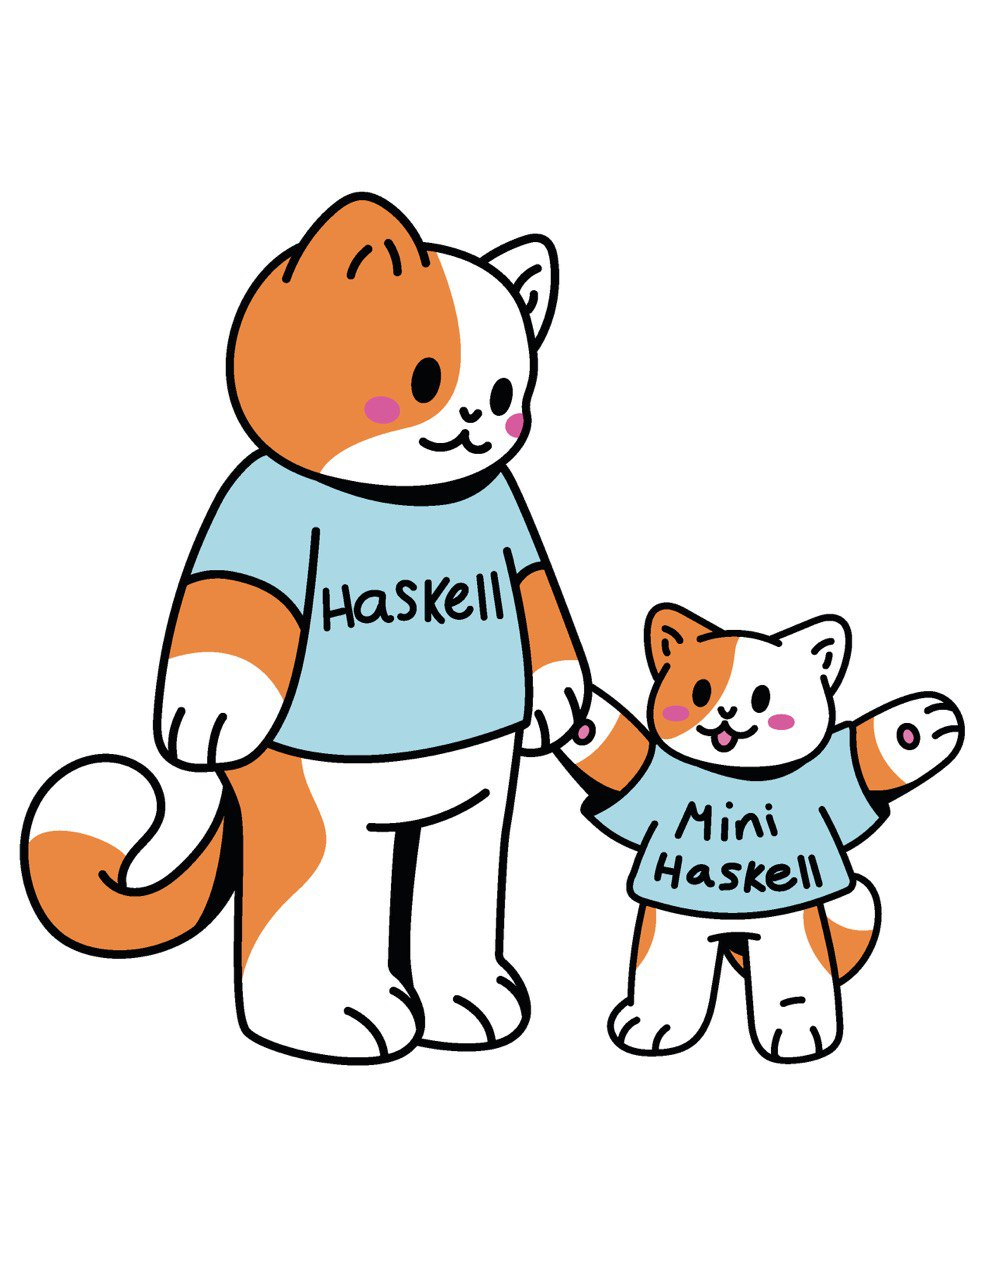
\includegraphics[scale=0.20]{assets/06_gatito_minHs.jpg}}       
\end{figure}

Con la teoría que hemos revisado hasta el momento en nuestro lenguaje \textsf{EAB} cuya definición engloba booleanos, a los números natures junto con sus operadores y la implementación del Cálculo Lambda, nos es natural preguntarnos  ¿cómo sería la implementación de un lenguje de características similares en una computadora?. Para resolver esta pregunta definiremos un lenguaje que contenga un subconjunto de instrucciones de algún otro lenguaje cuya implementación ya exista para computadoras.  \\\\
Por su naturaleza funcional tomaremos como caso de estudio una versión simplificada del lenguaje de programación \textsf{Haskell}. Este posee características deseables para el enfoque de este curso que serán de importancia trasladar a \textsf{EAB}. \\\\
Hasta el momento se ha trabajado con tipos de datos primitivos, pero no hemos hablado de la semántica estática que asigna dichos tipos a las expersiones, esto constituye un problema al poder escribir expresiones de \textsf{EAB} correctas pero cuya evaluación no termine en un valor puesto que la ejecución se detendría en algún momento al no hallar una regla de la semántica dinámica que nos permita continuar. \\\\
Con esto en mente el objetivo de este capítulo será definir un lenguaje similar que nos permita tener todos los tipos de datos de \textsf{EAB}, el sistema de tipos de \textsf{Haskell} y las características más importante del mismo, evaluación perezosa, pureza funcional y asignación de tipos explícita y estática. 
A este lenguaje lo llamaremos \textsf{MinHaskell} al ser menos robusto que su implementación para computadoras pero servirá para ilustrar los conceptos que hasta ahora hemos trabajado en este manual.

\subsubsection{Objetivo}
Proveer la definición del lenguaje funcional \textsf{MinHaskell} que preserve las características principales del lenguaje de programación \textsf{Haskell} a manera de ilustrar una implementación concreta de los conceptos que se han revisado hasta este momento: sintaxis, semántica, Cálculo Lambda y recursión, haciendo especial énfasis en el sistema de tipos de este lenguaje y sus propiedades.


\subsubsection{Planteamiento}
El desarrollo del capítulo se plantea de forma similar a como lo hemos hecho con el lenguaje \textsf{EAB} dividiendo su definición en sintaxis concreta, sintaxis abstracta, semántica dinámica y es aquí en donde se introducirá una nueva capa para estudiar la asignación de tipos de las expresiones. Finalmente concluiremos mencionando brevemente las propiedades que este pequeño lenguaje posee. \\

\section{sintaxis de MinHaskell}

\subsection{sintaxis concreta}
    Para construir el sistema de tipos de \textsf{MinHaskell}, se necesita introducir una nueva expresión de tipo al cual las variables pertenecen que será representado por la letra \textit{T}.\\\\    
     El tipo de las $\lambda$-expresiones  será representado por la expresión $T_1 \Rightarrow T_2$ en la sintaxis concreta donde $T_1$ representa el tipo de la variable ligada en el cuerpo de la expresión  y $T_2$ es el tipo que regresa la evaluación de la expresión. 

\bigskip

    Finalmente se introduce la expresión para funciones recursivas representadas por la expresión \textsf{letrec}$\; var=\; e_1\; {\sf in}\; e_2\;$ \textsf{end}
    \begin{definition}[Sintaxis Concreta de \textsf{MinHaskell}] A continuación definimos los elementos que componen a las expresiones válidas de \textsf{MinHaskell}.\footnote{Definición extraída de  \hyperlink{5}{[5]},  \hyperlink{12}{[12]}, \hyperlink{115}{[115]} y \hyperlink{116}{[116]}}\\ El tipo de las expresiones ahora figura como parte de la sintaxis concreta.
        \[
        \begin{array}{lrcl}
            \mbox{\bf Expresiones}&e&::=&\; var\; | \; n\; |\; b\; |\; (e)\; |\; e_1\otimes \; e_2\; |\; e_1 \; e_2\\
            &&|& \textsf{if} \;e_1\;{\sf then}\;e_2\;{\sf else}\;e_3\\
            &&|& \textsf{let} \;x=\;e_1\;{\sf in}\;e_2\;{\sf end}\\
            &&|& \textsf{lam} \; x :: \textit{T} \Rightarrow e \\
            &&|& \textsf{recfun} \;f :: (T_1\Rightarrow T_2)\; x \Rightarrow \;e\\
            \mbox{\bf Tipos}&\textit{T}&::=&\; \textit{Bool}\;|\textit{Nat}\;|\;T_1\Rightarrow T_2 \\
            \mbox{\bf Variables}&var&::=&x\; |\; y \; | \; \dots\\
            \mbox{\bf Números}&n&::=&0\; |\; 1 \; | \dots\\
            \mbox{\bf Booleanos}&b&::=&\textsf{True}\; |\; \textsf{False}\\
            \mbox{\bf Operadores Infijos}&\otimes&::=&+|*|-|=|<|>|\geq|\leq\\
        \end{array}
        \]
    \end{definition}

    \begin{exercise}
    Escribe la definición de los siguientes instrucciones utilizando la sintaxis concreta de \textsf{MinHaskell}\\

	\begin{itemize}
		\item Proporciona la definición de la función sucesor que recibe un número y regresa el sucesor \textsf{suc}: 
			$$ \textsf{lam}\; x\;::\; \textit{Nat} \rightarrow x + 1$$
		\item Proporciona la definición de la función que recibe un número y decide si es zero \textsf{IsZero}:
			 $$ \textsf{lam}\; x\;::\; \textit{Nat} \rightarrow\; \textsf{if}\; (x\; ==\; 0) \; \textsf{then}\; \textsf{True}\; \textsf{else}\; \textsf{False}$$
		\item Proporciona la definición de una función que recibe un número y regresa el factorial \textsf{fact}
			 $$ \textsf{recfun}\; \textsf{fact}\; ::\; (\textit{Nat} \rightarrow \textit{Nat})\; x \rightarrow\; \textsf{if}\; \textsf{IsZero}(x)\; \textsf{then}\; 1\; \textsf{else}\; n\; *\; \textsf{fact}\; (n-1)$$
		\item Proporciona la definición de una función que recibe dos números y regresa su producto \textsf{prod}:
			$$ \textsf{lam}\; x\; ::\; Nat \rightarrow\; \textsf{lam}\; y\; ::\; Nat \rightarrow\; x*y$$
	\end{itemize}

    \end{exercise}

\subsection{sintaxis abstracta}

    \begin{definition}[Sintaxis abstracta de \textsf{MinHaskell}]  Una vez definidas las reglas para generar programas en \textsf{MinHaskell} empleado la sintaxis concreta del lenguaje, podemos definir su representación intermedia empleado los árboles de sintaxis abstracta\footnote{Definición extraída de  \hyperlink{5}{[5]},  \hyperlink{12}{[12]}, \hyperlink{115}{[115]} y \hyperlink{116}{[116]}}.
    
        \begin{description}
            \item[Valores y variables]
        \[
            \begin{array}{ccc}
                \inference{n\in\N}{num[n]\;asa}&
                \inference{}{bool[\textit{True}]\;asa}&
                \inference{}{bool[\textit{False}]\;asa}
            \end{array}
        \]
        \[
            \begin{array}{ccc}
                \inference{x \in\ Variables}{x\;asa}
            \end{array}
        \]
        \item[Operadores]
        \[
            \begin{array}{c}
                \inference{t_1\;asa&\cdots&t_n\;asa}{o(t_1,\dots,t_n)\;asa}
            \end{array}
        \]
        \item[Condicional]
        \[
            \begin{array}{c}
                \inference{t_1\;asa&t_2\;asa&t_3\;asa}{if(t_1,t_2,t_3)\;asa}
            \end{array}
        \]
        \item[Asignaciones locales]
        \[
            \begin{array}{cc}
                \inference{t_1\;asa&t_2\;asa}{let(t_1,x.t_2)\;asa}&
            \end{array}
        \]
        \item[Definición de funciones]
        \[
            \begin{array}{c}
                \inference{t\;asa}{lam(\textit{T},x.t)\;asa}
                \inference{t\;asa}{recfun(T,f.x.t)\;asa}
            \end{array}
        \]
        \item[Aplicación de función]
        \[
            \begin{array}{c}
                \inference{t_1\;asa&t_2\;asa}{app(t_1,t_2)\;asa}
            \end{array}
        \]
        \item[Operador de punto fijo]
        \[
            \begin{array}{c}
                \inference{t\;asa}{fix(\textit{T},f.t)\;asa}
             \end{array}
         \]
		\[\]
    El operador de punto fijo $fix$ es una implementación interna para evaluar expresiones recursivas. Como no está asociado a ninguna expresión de la sintaxis concreta es imposible que un usuario lo pueda instanciar directamente.\\\\
    El operador $recfun$ tiene dos variables ligadas en el cuerpo de la definición: el nombre de la función y la variable que recibe como argumento.
        \end{description}
    \end{definition}

\section{Semántica de MinHaskell}

    \subsection{Sistemas de tipos}
    Los tipos en el contexto de los lenguajes de programación son la descripción abstracta de una colección de valores que nos permite agruparlos y emplearlos de manera similar aún sin saber el contentido específico que este pudiera tener.\\\\
    En los lenguajes de programación los sistemas de tipos brindan información adicional sobre la evaluación de las expresiones, qué valores debemos esperar recibir y regresar al concluir la ejecución de nuestro programa para definir restricciones que nos permitan tener seguridad y congruencia en los datos empleando una colección de reglas de tipado.\\\\
    Este sistema estará embedido en la siguiente capa de \textsf{MinHaskell} de forma similar como fue trabajado con anterioridad con el lenguaje \textsf{EAB}, dicho nivel es la semántica estática que define un conjunto de juicios para brindar la seguridad de evaluación a las expresiones.

\subsection{Semántica estática}

    \textsf{Haskell} es un lenguaje de programación categorizado como fuertemente tipado, esto quiere decir que la evaluación de las expresiones solo es posible cuando el programa es congruente con las reglas definidas por su sitema de tipos, descartando la evaluación de todas aquellas expresiones que estén bien formadas pero que no respeten las restricciones del sistema. \\


    \begin{definition}[Semántica estática]
       La semántica estática nos ayuada a definir criterios para evaluar los programas de \textsf{MinHaskell} con la información que se pueda inferir acerca de los parámetros que una expresión toma como argumento o el tipo que esta regresa al concluir su evaluación\footnote{Definición extraída de  \hyperlink{5}{[5]},  \hyperlink{12}{[12]}, \hyperlink{115}{[115]} y \hyperlink{116}{[116]}}. Para este propósito definimos el siguiente juicio:
    
    $$\Gamma\vdash t: T$$
    
    \noindent
    El cual se lee como: ''la expresión $t$ tiene tipo T$\ $bajo el contexto $\Gamma$''. 
    En donde $\Gamma$ es un conjunto de asignaciones de tipos a variables de la forma $\{x_1:T_1\dots x_n:T_n\}$\footnote{Se utiliza la notación $\Gamma, x:T$ para indicar el conjunto $\Gamma \cup \{x:T\}$}.
        \begin{description}
            \item[Variables]
            \[
                \inference{}{\Gamma, x:T\vdash x:T}
            \]
            \item[Valores numéricos]
            \[
                \inference{}{\Gamma\vdash num[n] : \textit{Nat}}
            \]
             \item[Valores Booleanos]
             \[
                \begin{array}{ccc}
                    \inference{}{\Gamma\vdash bool[\textit{False}] :\textit{Bool}}&\quad&
                    \inference{}{\Gamma\vdash bool[\textit{True}] :\textit{Bool}}
                \end{array}
            \]
            \item[Operadores]
            \[
                \begin{array}{ccc}
                    \inference{\Gamma\vdash t_1:nat&\Gamma\vdash t_2: \textit{Nat}}{\Gamma\vdash sum(t_1,t_2) : \textit{Nat}}&
                    \quad&
                    \inference{\Gamma\vdash t_1:nat&\Gamma\vdash t_2: \textit{Nat}}{\Gamma\vdash prod(t_1,t_2) : \textit{Nat}}\\
                    &&\\
                    \inference{\Gamma\vdash t_1:nat&\Gamma\vdash t_2: \textit{Nat}}{\Gamma\vdash sub(t_1,t_2) : \textit{Nat}}&
                    \quad&
                    \inference{\Gamma\vdash t_1:nat&\Gamma\vdash t_2: \textit{Nat}}{\Gamma\vdash ig(t_1,t_2) : \textit{Bool}}\\
                    &&\\
                    \inference{\Gamma\vdash t_1:nat&\Gamma\vdash t_2: \textit{Nat}}{\Gamma\vdash gt(t_1,t_2) : \textit{Bool}}&
                    \quad&
                    \inference{\Gamma\vdash t_1:nat&\Gamma\vdash t_2: \textit{Nat}}{\Gamma\vdash lt(t_1,t_2) : \textit{Bool}}\\
                \end{array}
            \]
            \item[Condicional]
            \[
                \inference{\Gamma\vdash t_c:\textit{Bool}&\Gamma\vdash t_t:T&\Gamma\vdash t_e:T}{\Gamma\vdash if(t_c,t_t,t_e):T}
            \]
            \item[Asignaciones Locales]
            \[
                \begin{array}{ccc}
                    \inference{\Gamma\vdash t_v:T&\Gamma,x:T\vdash t_b:St}{\Gamma\vdash let(t_v,x.t_b) : St}&\quad&
                \end{array}
            \]
            \item[Funciones]
            \[
                \inference{\Gamma,x:T\vdash t:St}{\Gamma\vdash fun(T,x.t): T\to St} \quad
                \inference{\Gamma\vdash f:T\to St,x : T \vdash t : S}{\Gamma\vdash recfun(T \to S,f.x.t):T\to S}
            \]
            \item[Aplicación de función]
            \[
                \inference{\Gamma\vdash t_f:T\to St&\Gamma\vdash t_p : T}{\Gamma\vdash app(t_f,t_p):St}
            \]
            \item[Operador de punto fijo]
            \[
                \inference{\Gamma,x:T\vdash t:T}{\Gamma\vdash fix(T,x.t):T}
            \]
            Obsérvese que en el caso de $fix\,$ se está asumiendo el mismo tipo que se debe concluir.
        \end{description}
    \end{definition}

    \begin{exercise}
        Para cada expresión de $MinHaskell$ enlistada a continuación obtén su representación en \textbf{sintaxis abstracta} y aplica las reglas de la \textbf{semántica estática} para hacer el análisis de tipos de la expresión.\\\\
        % USA DESCRIPTION
        % \begin{description}
        %   \item[Representación en sintaxis concreta]
        % \end{description}
        \textbf{Representación en sintaxis concreta: }
        $$ 1\ +\ (7\ -\ 1)$$
        \textbf{Representación en sintaxis abstracta: }
        $$ sum(num[1],res(num[7],num[1]))$$
        \textbf{Análisis de tipo aplicando la semántica estática: }
        $$\inference{\inference{}{\empty \vdash num[1]\ :\textbf{Nat}} & \inference{\inference{}{\empty \vdash num[7]\ :\ \textbf{Nat}} & \inference{}{ \empty \vdash num[1]\ :\ \textbf{Nat}}}{\empty \vdash res(num[7],num[1])\ :\ \textbf{Nat}}}{ \empty \vdash sum(num[1],res(num[7],num[1])) : \textbf{Nat}}$$
        \textbf{Representación en sintaxis concreta: }
        $$ lam\ x\ :: \textbf{Nat} \rightarrow\ x\ \textgreater\ 1$$
        \textbf{Representación en sintaxis abstracta: }
        $$  fun(\textbf{Nat}, x.gt(x,num[1]))$$
        \textbf{Análisis de tipo aplicando la semántica estática: }
        $$  \inference{\inference{\inference{}{x\ :\ Nat \vdash  x\ :\ \textbf{Nat}} & \inference{}{x\ :\ Nat \vdash num[1]\ :\ \textbf{Nat}}}{x\ :\ Nat \vdash gt(x,num[1]) : \textbf{Bool}}}{\empty \vdash fun(\textbf{Nat}, x.gt(x,num[1]))\ :\ \textbf{Bool} \to \textbf{Nat}} $$
        \textbf{Representación en sintaxis concreta: }
        $$ \textbf{let}\ x\ =\ 3\ \textbf{in}\ if\ x \textless 7\ \textbf{then}\ x\ +\ (7\ -\ x)\ \textbf{else}\ x\ \textbf{end} $$
        \textbf{Representación en sintaxis abstracta: }
        $$  let(num[3],x.if(lt(x,num[7]),num[7],sum(x,res(num[7],x))))$$
        \textbf{Análisis de tipo aplicando la semántica estática: }
        $$\scalemath{0.7}{
            \inference{\inference{}{\vdash num[3]\ :\ \textbf{Nat}} & \inference{ \inference{(A) \cdots}{x:\textbf{Nat} \vdash lt(x,num[7]) : \textbf{Bool}} & \inference{}{x:\textbf{Nat} \vdash num[7] : \textbf{Nat}} & \inference{(B) \cdots}{x:\textbf{Nat} \vdash sum(x,res(num[7],x)) : \textbf{Nat}}}{x:\textbf{Nat} \vdash if(lt(x,num[7]),num[7],sum(x,res(num[7],x)) }}{\empty \vdash let(num[3],x.if(lt(x,num[7]),num[7],sum(x,res(num[7],x))))\ :\ \textbf{Nat}}
        }$$
        \textbf{(A) Análisis semántico para lt}
        $$ \inference{\inference{}{x:\textbf{Nat} \vdash x:\textbf{Nat}} & \inference{}{x:\textbf{Nat} \vdash num[7] : \textbf{Nat}}}{x:\textbf{Nat} \vdash lt(x,num[7]) : \textbf{Bool}} $$
        \textbf{(B) Análisis semántico para sum}
        $$ \inference{\inference{}{x:\textbf{Nat} \vdash x:\textbf{Nat}} & \inference{\inference{}{x:\textbf{Nat} \vdash num[7] : \textbf{Nat}} & \inference{}{x:\textbf{Nat} \vdash x:\textbf{Nat}}}{x:\textbf{Nat} \vdash res(num[7],x) : \textbf{Nat}}}{x:\textbf{Nat} \vdash sum(x,res(num[7],x)) : \textbf{Nat}} $$
    \end{exercise}

\subsection{Semántica dinámica}

    Para concluir con la definición de $MinHaskell$ enunciaremos las reglas de la \textbf{Semántica Operacional}. Es importante observar que la evaluación perezosa característica de \textbf{Haskell} se debe particularmente a los operadores \textbf{app} y \textbf{let} dado que la sustitución se hace sin evaluar la expresión que dará el valor en la variable ligada. 
    \begin{definition}[Semántica Operacional de paso pequeño perezosa]
        \begin{itemize}
            \item Conjunto de estados $S=\{a\;|\;a\;asa\}$
            \item Estados Iniciales $I=\{a\;|\;a\;asa,\;\varnothing\sim a\}$
            \item Estados Finales $F = \{num[n],bool[true],bool[false],lam(x.t)\}$
            \item Transiciones, dadas por las siguientes reglas:
            \begin{description}
                \item[Condicional]
    
                \[
                    \begin{array}{ccc}
                        \inference{}{if(bool[true],a_t,a_e)\to a_t}[\sf ifT]&\quad&
                        \inference{}{if(bool[false],a_t,a_e)\to a_e}[\sf ifF]
                        \quad
                    \end{array}
                \]
                \[
                    \begin{array}{c}
                        \inference{a_c\to a_c'}{if(a_c,a_t,a_e)\to if(a_c',a_t,a_e)}[\sf if]
                        \quad
                    \end{array}
                \]
    
                \item[Asignaciones locales]
    
                \[
                    \begin{array}{c}
                        \inference{}{let(a_1,x.a_2)\to a_2[x:=a_1]}[\sf let]\\
                    \end{array}
                \]
    
                \item[Aplicación de función]
                \[
                    \begin{array}{ccc}
                        \inference{}{app(lam(x.a_b),a_p)\to a_b[x:=a_p]}[\sf app]&
                    \end{array}
                \]
                \[
                    \begin{array}{ccc}
                        \inference{a_f \to a_f'}{app(a_f,a_p)\to app(a_f',a_p)}[\sf appL]\
                    \end{array}
                \]
                \[
                    \begin{array}{ccc}
                        \inference{}{app(recfun(\textbf{T},x.a_b),a_p) \to a_b[f:=fix(\textbf{T},f.x.a_b),\ x:=\ a_p])}[\sf appR]\
                    \end{array}
                \]
                $$$$
                \[
                    \begin{array}{ccc}
                        \inference{}{app(fix(\textbf{T},f.x.a_b),a_p) \to a_b[f:=fix(\textbf{T},f.x.a_b),x:=a_p]}[\sf appF]\
                    \end{array}
                \] 
                \item[Operador de punto fijo]
                \[
                    \begin{array}{c}
                        \inference{}{fix(\textbf{T},f.a) \to a[f := fix(\textbf{T},f.a)]}[\sf fix]
                    \end{array}
                \]
                \item[Operadores] 
                    $$$$
                     \text{Para acotar el listado de reglas se omite la representación para los} \\
                     \text{operadores cuya definición es la misma a la que se dió para \emph{EAB} en} \\
                     \text{el \textbf{Capítulo 4: Semánitca} definición 2.3, las reglas para operadores} \\
                     \text{booleanos de comparación $lt,\ \textless, \textgreater, =$ se define de manera análoga.}
            \end{description}
        \end{itemize}
\end{definition}

\section{Propiedades de MinHaskell}

    Para concluir este capítulo revisaremos brevemente las propiedades que la definición de $MinHaskell$ posee. Mas adelante revisitaremos esta sección para discutir el resto de éllas enunciando únicamente las propiedades \textbf{Seguridad} y \textbf{No terminación} del lenguaje.

    \subsection{Seguridad del lenguaje}
        Esta propiedad es una característica que nos ayuda a verificar la correctud del sistma, y se interpreta como: "Un programa que cumpla con las restricciones dadas por el sistema de tipos no puede tener una evaluación errónea". Ligándo las definiciones para la \textbf{Semánitca estática} conciernente al tipado de las expresiones y la \textbf{Semánitca Dinámica} concerniente a la evluación de las mismas.\\
        
        Ésta propiedad posse dos características que se aplican a las expresiones de $MinHaskell$:
        \begin{itemize}
            \item \textbf{Progreso} \\
            Engloba la propiedad: "Un programa que cumple con las restricciones de tipado no se bloquea hasta llegar a un valor." Éste comportamiento está capturado en la definición de progreso enlistada a continuación para las expresiones de $MinHaskell$:\\
             
             \begin{definition}[Propiedad de progreso]
                Si $\vdash t : \textbf{T}$ para algún tipo \textbf{T} entonces se cumple una de los siguientes dos casos:\\
                (A) t es un valor \\
                (B) Existe una expresión t' tal que t $\to$ t'
             \end{definition}
                $$$$
            \item \textbf{Preservación} \\
                Referente a la idea: "Un programa que cumple con las restricciones de tipado dará como resultado de la evaluación una expresión correctamente tipada y que potencialmente preserva su mismo tipo"\\
        
                Ésto se puede observar en las siguientes dos propiedades definidas para las expresiones de $MinHaskell$:\\
                

                    \begin{definition}[Unicidad de tipado]
                        Para cualesquiera $\Gamma$ y expresión t de \textbf{MinHs} existe a lo más un tipo \textbf{T} de tal forma que se cumple: $\Gamma \vdash t : \textbf{T}$\\    
                    \end{definition}
                    
                     \begin{definition}[Preservación de tipos]
                        Sí $\Gamma \vdash t : \textbf{T}$ y $t \to t'$ entonces $\Gamma \vdash t' : \textbf{T}$
                    \end{definition}

        \end{itemize}

    \subsection{No terminación}
        $MinHaskell$ hereda un problema similar a lo que sucedió en el \textbf{Cálculo Lambda} con la introducción de los combinadores para implementar la \textbf{recursión general}. Éste problema es la existencia de expresiones del lenguaje sintácticamente y semánticamente correctas que producen un estado conocido \textbf{´loop´} ó \textbf{'estado de ciclado'}


        \begin{exercise}
            Demuestra o da un contraejemplo de la propiedad de no terminación para $MinHaskell$\\

            Considera la función identidad que recibe un parámetro y regresa el mismo representada como \textbf{x.x} sí utilizamos esta expresión como el cuerpo de nuestro operador \textbf{fix} obtenemos la expresión:
            \[
                fix(x.x) \to x[x:=fix(x.x)] = fix(x.x) \to ... \footnote{Ejemplo extraido de Javier E. Mendoza, Lenguajes de Programación 2023-1 Nota de clase 6 \textbf{MinHaskell}, Universidad Nacional Autónoma de México. pp 8}
            \]
            Por lo tanto $MinHaskell$ \textbf{no posee} la propiedad de terminación.
            
        \end{exercise}


\newpage

\section{Ejercicios para el lector}

    Para concluir el capítulo se enlistan a continuación los ejercicios de comprensión para el lector, similares a los revisados durante el capítulo.\\\\
    Estos ejercicios pretenden aplicar los diferentes niveles de la semánitca y la sintaxis de $MinHaskell$ agregando instrucciones para el lenguaje o verificando el tipado sobre la definición de funciones y expresiones\footnote{Ejercicios \textbf{4.3}, \textbf{4.5} y \textbf{4.6} extraídos de Javier E. Mendoza, Kevin P. Ramos, Lenguajes de Programación 2023-1; Boletín de ejercicios 4, Noviembre 2022. Extendiendo la definición del operador \textbf{Case} para incluir el caso por omisión.}.

    \bigskip

    \begin{exercise}
        Queremos extender la definición de $MinHaskell$ para agregar el tipo de dato algebráico $tupla$ representado como \textbf{Pair(x,y)} (donde ambos elementos no necesariamente tienen que tener el mismo tipo). Así como las proyecciones \textbf{Fst} y \textbf{Snd}.\\

        Con  la descripción anterior responde los siguientes puntos:
        \begin{itemize}
            \item Define la sintaxis concreta para las tuplas.
            \item Define la regla de sintaxis abstracta para las tuplas.
            \item Define la regla de la semántica estática para las tuplas.
            \item Define la(s) reglas de evluación para las tuplas.
            \item Cuál es la diferencia entre una expresión que construye la tupla y la proyección que obtiene el elemento? (\textbf{Hint: } Las reglas de la semántica dinámica permiten comparar ambos elementos para responder este punto).
        \end{itemize}
    \end{exercise}

    \bigskip

    \begin{exercise}
        Para las siguientes expresiones de $MinHaskell$ determina el tipo y verifica tu respuesta utilizando las reglas de la \textbf{Semántica estática}.\\
        
        \begin{itemize}
            \item \textbf{Pair(3, True)}
            \item \textbf{Snd Pair(3, True)}
            \item \textbf{app(lam(Nat, x.suc(x)), 0)}  
            \item  \textbf{$recfun\; fact\; ::\; (\textbf{Nat} \rightarrow \textbf{Nat})\; x \rightarrow\; if\; IsZero(x)\; then\; 1\; else\; n\; *\; fact\; (n-1)$}
            \item  \textbf{$ let\; f\; ::\; (\textbf{Nat} \rightarrow \textbf{Nat})\; in\; lam\; x\; ::\; Nat \rightarrow\; f\; x\; end$}
        \end{itemize}
    \end{exercise}

    \begin{exercise}
        El operador \textbf{Case $x$ of $x.g \rightarrow\ c1$ ; $x.g \rightarrow\ c2$ ; ... end} es la generlización de múltiples expresiones \textbf{if} \textbf{else} para evaluar el argumento de entrada o $guardia$ ($g$) y el caso al que este es aplicado ($e_n$) de tal forma que se toma como resultado de la expresión la primera guardia que se evalúe a verdadero de izquierda a derecha (o de arriba hacia abajo como generalmente se escribe el operador \textbf{Case}). \\\\
        Adicionalmente queremos definir una expresión que por omisión sea el resultado del \textbf{Case} en caso de que ninguna de las condicionales se evalúe a verdadero: 
        $$ \textbf{ Case } x \textbf{ of } x.g \rightarrow\ c1\ ;\ x.g \rightarrow\ c2\ ;\ ...\ ;\ e_d\ \textbf{end} $$

        Con la especificación dada anterior contesta los siguientes incisos:
        \begin{itemize}
            \item Extiende la sintaxis concreta del lenguaje para el operador \textbf{Case} (\textbf{Hint:} se puede añadir un nivel extra para las expresiones guardadas y la expresión \textbf{default}).
            \item Extiende la sintaxis abstracta del lenguaje para el operador \textbf{Case}. 
            \item Extiende la semántica estática del lenguaje para el operador \textbf{Case}. 
            \item Extiende la semántica dinámica del lenguaje para el operador \textbf{Case} (recuerda que se tiene que seguir la implementación de evaluación perezosa).
        \end{itemize}
    \end{exercise}

    \begin{exercise}
        Dada la siguiente expresión \textbf{Case}: 
        $$ \textbf{Case } n \textbf{ of }  n \textless 0 \rightarrow \textbf{ True } ; n = 0 \rightarrow \textbf{ True } ; \textbf{ False }$$
        \begin{itemize}
            \item Evalúala utilizando las reglas de semántica dinámica definidas en el inciso anterior.
            \item Sí $\Gamma = \{n:\textbf{Nat}\}$ utiliza las reglas de semántica estática definidas en el inciso anterior para obtener el tipado de la expresión.
        \end{itemize}
    \end{exercise}

    \begin{exercise}
        Define las siguientes funciones utilizando la sintaxis concreta de $MinHaskell$ y aplica las reglas de la semántica estática para verificar el tipado de las mismas.
        \begin{itemize}
            \item Define la función \textbf{exp}($n_1\ $ $n_2)$ que eleva el primer argumento a la potencia del segundo.
            \item Define la función \textbf{fibonacci}(n) que obtiene el n-ésimo elemento de la sucesión de Fibonacci.
            \item Evalúa la expresión \textbf{exp}(2,2) y \textbf{fibonacci}(3).
        \end{itemize}
    \end{exercise}

    \begin{exercise}
        Para las siguientes expresiones, verifique el tipado mostrando la derivación mediante la semántica estática.
        \begin{itemize}
            \item (\textbf{fun} x : \textbf{Nat $\to$ Nat} $\rightarrow$ (\textbf{fun} w : \textbf{Nat} $\rightarrow$ (x w) + (x w))) (\textbf{fun} y : \textbf{Nat} $\rightarrow$ y + 1) 
            \item (\textbf{let} neg = (\textbf{fun} x : \textbf{Bool} $\rightarrow$ \textbf{if } x \textbf{then } false \textbf{else} true) \textbf{in} neg(3 $\leq$ 2) \textbf{end})
        \end{itemize}
    \end{exercise}


%https://www.cs.princeton.edu/~dpw/cos441-11/notes/slides15-lambda-proofs.pdf
		
		\chapter{Inferencia de tipos}
			%    Séptimo Capítulo: Inferencia de Tipos.
%    Ejercicios por Barón L. Miguel.
%    Teoría por Javier Enríquez Mendoza.
%    Empezado el 12/4/23
%    Concluido el 1/6/23
% https://www.webber-labs.com/wp-content/uploads/2015/08/mpl-06.pdf
% http://www.dcc.ic.uff.br/~isabel/LP/D.Watt.pdf
% https://www.cs.cornell.edu/courses/cs3110/2011sp/Lectures/lec26-type-inference/type-inference.html
% https://rodrigogribeiro.github.io/files/unify.pdf
% file:///C:/Users/luismun/Downloads/doiufrgs,+100968-426558-3-CE.pdf https://www.google.com/url? sa=t&rct=j&q=&esrc=s&source=web&cd=&ved=2ahUKEwiPy8-9842HAxVeD1kFHf_rB7Q4ChAWegQIIBAB&url=https%3A%2F%2Fwww.seer.ufrgs.br%2Frita%2Farticle%2Fdownload%2FVol27_nr3_13%2Fpdf_1&usg=AOvVaw0CRZfNvzqWmtheLBDCOXwk&opi=89978449

%Gatito lambda
\begin{figure}[htbp]
    \centerline{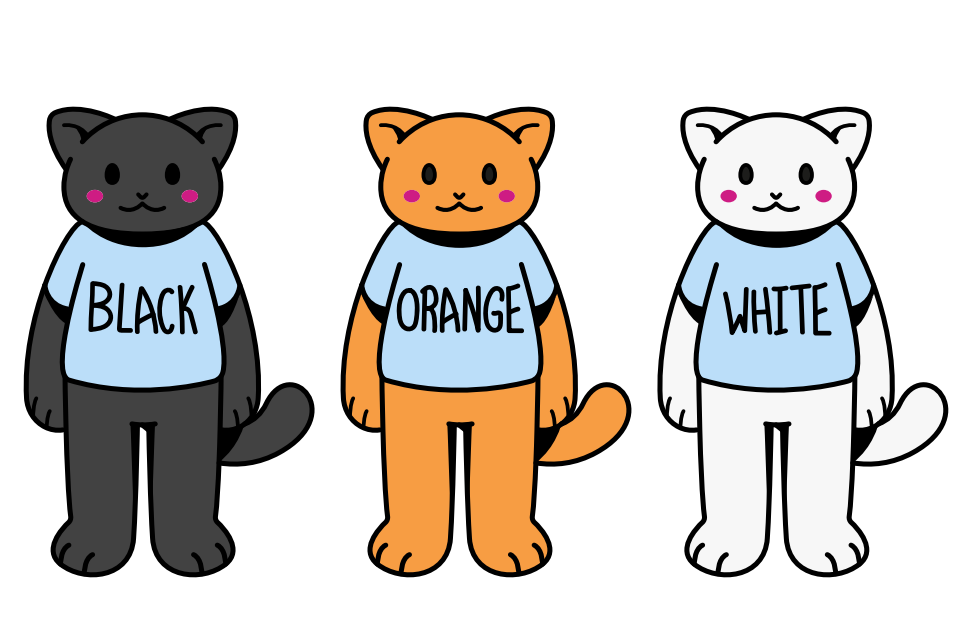
\includegraphics[scale=0.5]{assets/gatitos_tipados.PNG}}       
\end{figure}

Una característica de \textsf{Haskell} que quermos trasladar a \textsf{MinHS} es el mecanismo de inferencia de tipos. Este mecanismo provee una capa extra que permite trabajar con expresiones aún si estas no poseen un tipo explicito en cada uno de sus parámetros de entrada y valores de retorno. \\\\
Para esto, vamos a formular un sistema de restricciones, la estandarización de variables y aplicación de la inferencia de tipos mediante el algoritmo de unificación de tipos para expresiones de \textsf{MinHS}.\\\\
Anteriormente se defininieron mediante la semantíca estática las reglas para obtener el tipo de una expresión, no obstante este proceso no es suficiente para descartar expresiones del lenguaje bien formadas pero cuya evaluación se verá detenida debido a la inconsistencia de tipos durante la evaluación.\\\\
Esta nueva capa aporta a que al lenguaje se vuelva seguro, es decir que si una expresión de \textsf{MinHS} está bien formada y ha sido tipificada siguiendo las diferentes reglas y etapas correctamente entonces nuestro programa nos regresará un valor.\\

\subsubsection{Objetivo}
Definir el sistema de inferencia de tipos para \textsf{MinHS} que nos permita tipificar las expresiones para garantizar la seguridad del lenguaje. Para esto, el objetivo principal será proporcionar las definiciones para las condiciones que cada estructura particular de las expresiones sintácticas de \textsf{MinHS} generan, a estas se les conoce como restricciones de tipo. Adicionalmente se proporcionará la definción del algoritmo de unificación para aplicar la inferencia de tipos conocido como algoritmo  unificador \textbf{$\mu$}.


\subsubsection{Planteamiento}
En este capítulo  revisaremos diferentes  procedimientos que se aplican a las expresiones de \textsf{MinHS} para poder garantizar la correcta  asignación de un tipo.
Estudiaremos la estandarización de variables para obtener $\alpha\text{-equivalencias}$ entre las variables ligadas repetidas dentro de una expresión.
Posteriormente vamos a revisar los juicios para generar las restricciones de tipo que cada expresión genera para finalmente definir el algoritmo unificador $\mu$.


\section{Estandarización de variables}
La semántica estática de \textsf{MinHS} y la de \textsf{EAB} se implementa de forma similar para ir agregando a un contexto (que denotaremos con la letra $\Gamma$) aquellas variables definidas en las expresiones junto con el tipo que se espera estas tengan.\\\\
En el contexto $\Gamma$ solo puede existir una sola aparición por variable, es decir, nunca podremos tener $\Gamma=\{x : Nat,\ x : Bool\}$ dado que $\Gamma$ es un conjunto de variables y tipos, tener la misma variable con dos tipos distintos es una inconsistencia dentro de nuestro programa y constituye un error en el tipificado de la expresión\footnote{Definición de semántica estática para \textsf{MinHS} formulada de  \hyperlink{5}{[5]},  \hyperlink{12}{[12]}, \hyperlink{115}{[115]} y \hyperlink{116}{[116]}}.\\\\
Para evitar esta situación se define el proceso conocido como estandarización de variables que consiste en brindar una $\alpha$-equivalencia cuando dos variables ligadas tengan el mismo nombre.\\\\
Tomemos como ejemplo la siguiente expresión:
$$ \textsf{let } x = \textsf{True} \textsf{ in } x\ !=\ \textsf{ let } x = 5 \textsf{ in } x \leq x \textsf{ end } \textsf{ end }$$
En este caso la expresión está bien formada, no hay ninguna regla de la sintáxis concreta que esté mal aplicada para obtener nuestra expresión, la evaluación tampoco comprende un problema dado que la expresión \textsf{let} mas interna se evalúa a a verdadero y luego se prosigue con la comparación de dos booleanos, sin embargo esta expresión nos genera el contexto $\Gamma=\{x : Nat,\ x : Bool\}$ el cual es inconsistente.\\\\
El problema puede ser corregido utilizando una $\alpha$-equivalencia y renombrando las variables x por $x_0$ y $x_1$ respectivamente:
$$ \textsf{let } x_0 = \textsf{True} \textsf{ in } x_0\ !=\ \textsf{ let } x_1 = 5 \textsf{ in } x_1 \leq x_1 \textsf{ end } \textsf{ end }$$
Donde el contexto obtenido será: $\Gamma=\{x_1 : Nat,\ x_0 : Bool\}$

\begin{exercise}
    Para la siguiente expresión de \textsf{MinHS} expresando el contexto
    $$\textsf{let } x = \textsf{False} \textsf{ in } x = (\textsf{let } x = 6 \textsf{ in } (x + x + x) \leq 10 \textsf{ end}) \textsf{ end }$$
    $$\Gamma=\{x : Nat,\ x : Bool\}$$
    
    Aplica la estandarización de variables:
    
    $$\textsf{let } x_0 = \textsf{False} \textsf{ in } x_0 == (\textsf{let } x_1 = 6 \textsf{ in } (x_1 + x_1 + x_1) \leq 10 \textsf{ end}) \textsf{ end }$$
    $$\Gamma=\{x_1 : Nat, x_0 : Bool\}$$

\end{exercise} 

\begin{exercise}    
    Para la siguiente expresión de \textsf{MinHS} expresando el contexto

    $$ \textsf{let } x = \textsf{True} \textsf{ in } x \textsf{ or } (\textsf{let } x = 5 \textsf{ in } x == 5 \textsf{ end}) \textsf{ end} $$
    $$ \Gamma = \{x:Bool,\ x:Nat\}$$
    
    Aplica la estandarización de variables: 
    
    $$ \textsf{let } x_0 = \textsf{True} \textsf{ in } x_0 \textsf{ or } (\textsf{let } x_1 = 5 \textsf{ in } x_1 = 5 \textsf{ end}) \textsf{ end} $$
    $$ \Gamma = \{x_1:Bool,\ x_0:Nat\}$$
\end{exercise}

\begin{exercise}    
    Para la siguiente expresión de \textsf{MinHS}, expresando el contexto
    
    $$ \textsf{let } x = 1 \textsf{ in } (\textsf{let } x = \textsf{False} \textsf{ in } (\textsf{let } x = lam\ y :: Bool \to y  \textsf{ or } x \textsf{ end }) \textsf{ end}) \textsf{ end }$$
    $$ \Gamma = \{ x : Int, x : Bool,\ x : Bool \to Bool \}$$
    
    Aplica la estandarización de variables:
    
    $$ \textsf{let } x_0 = 1 \textsf{ in } (\textsf{ let } x_1 = \textsf{False} \textsf{ in } (\textsf{let } x_2 = lam\ y :: Bool \to y  \textsf{ or } y \textsf{ end}) \textsf{ end}) \textsf{ end} $$
    $$ \Gamma = \{ x_0 : Int,\ x_1 : Bool,\ x_2 : Bool \to Bool \}$$
\end{exercise}

\section{Generación de restricciones}

    Para poder tipificar una expresión bien formada de \textbf{MinHS}  sin utilizar las anotaciones de tipo explicitamente en los argumentos y valores de retorno es necesario definir un proceso que nos ayude a obtener información sobre la estructura que esta posee. \\\\
    A esta información se le conoce como restricciones y nos ayuda a atar las condiciones que se deben cumplir para aplicar los procesos de inferencia de tipos.

    \begin{definition}[Conjunto de restricciones]
        Definimos el jucio para generar restricciones partiendo de una expresión válida $e$ representado como\footnote{Jucio para representar restricciones \hyperlink{123}{[123]},  \hyperlink{124}{[124]} y \hyperlink{125}{[125]}}:
    
        $$e\mapsto\R$$
        
        que se lee como: "la expresión $e$ genera el conjunto $\R$ de restricciones de tipo".
    \end{definition}

    \begin{definition}[Extensión de tipos para la generación de restricciones]
        Para definir el algoritmo se extiende la categoría de tipos como sigue\footnote{Definición formulada de \hyperlink{5}{[5]},  \hyperlink{12}{[12]}, \hyperlink{125}{[125]} y \hyperlink{124}{[124]}}:
        
        $$\ T\ ::=\ X\ |\ Nat\ |\ Bool\ |\ T_1\ \to T_2\ |\ [e]$$
        
        En donde $X$ $\,$ es una variable de tipo. Estas variables nos ayudan en la definición de programas polimórficos, por ejemplo la función identidad:
        
        $$lam\ x\Rightarrow x :: X \to X$$ 
        
        La variable de tipo $X$$\,$ va a tomar su valor hasta que la función sea evaluada, por ejemplo en la aplicación:
       
        $$(funt\ x \Rightarrow x)\ 5 :: Nat \to Nat$$

        La expresión [$e$] es una construcción sintáctica para definir el tipo de una expresión $e$ del lenguaje y se lee como: ''el tipo de $e$''. Es importante aclarar que los tipos de la forma [$e$] no pueden figurar en el tipo resultante del algoritmo de unificación $\mu$.  
            
    \end{definition}

   \bigskip    


    \begin{definition}[Algoritmo de generación de restricciones]
    
    Una restricción es una ecuación de la forma $T_1 = T_2$ en donde $T_1$ y $T_2$ son tipos. La ecuación indica que $T_1$ debe ser igual a $T_2$ bajo unificación\footnote{Definición formulada de \hyperlink{5}{[5]},  \hyperlink{12}{[12]}, \hyperlink{125}{[125]} y \hyperlink{124}{[124]}}.\\

        \begin{description}
            \item[Variables]
            \[
                \inference{}{x_i\mapsto [x_i] = X_i}
            \]
            Para el tipo de las variables se usará una variable de tipo con el mismo nombre de la variable. Todas las apariciones de la misma variable generarán la misma restricción y como los nombres de variables son únicos no habrá dos variables distintas con el mismo tipo. 
            \item[Valores numéricos]
            \[
                \inference{}{num[n] \mapsto [num[n]] = Nat}
            \]
             \item[Valores Booleanos]
             \[
                \inference{}{bool[b] \mapsto [bool[b]] = Bool}
            \]
            \item[Condicional]
            \[
                \inference
                    {c \mapsto R_1 & t \mapsto R_2 & e \mapsto R_3}
                    {if(c,t,e) \mapsto R_1, R_2, R_3, [c] = Bool, [t] = [e], [if(c,t,e)] = [e], [if(c,t,e)] = [t]}
            \]
            \item[Asignaciones Locales]
            \[
                \begin{array}{c}
                    \inference
                        {v \mapsto R_1 & b \mapsto R_2}
                        {let(v,x_i.b) \mapsto R_1, R_2, X_i = [v], [let(v,x_i.b)] = [b]}\\
                    \\
                    \inference
                        {v \mapsto R_1 & b \mapsto R_2}
                        {letrec(v,x_i.b) \mapsto R_1, R_2, X_i = [v],[letrec(v,x_i.b)] = [b]}\\
                \end{array}
            \]
            \newpage
            \item[Funciones]
            \[
                \inference
                    {t \mapsto R}
                    {funt(x_i.t) \mapsto R,[funt(x_i.t)] = X_i \to [t]}
            \]
            \item[Aplicación de función]
            \[
                \inference
                    {f \mapsto R_1 & p \mapsto R_2}
                    {app(f,p) \mapsto R_1, R_2, [f] = [p] \to [app(f,p)]}
            \]
            \item[Operadores]
            \[
                \begin{array}{c}
                    \inference
                        {e_1 \mapsto R_1 & e_2 \mapsto R_2}
                        {sum(e_1 , e_2) \mapsto R_1,R_2, [e_1] = Nat, [e_2] = Nat, [sum(e_1 , e_2)] = Nat}\\
                    \\
                     \inference
                        {e_1 \mapsto R_1 & e_2 \mapsto R_2}
                        { prod(e_1 , e_2) \mapsto R_1, R_2, [e_1] = Nat, [e_2] = Nat, [prod(e_1 , e_2)] = Nat}\\
                    \\
                     \inference
                        {e_1\mapsto R_1 & e_2 \mapsto R_2}
                        { sub(e_1,e_2) \mapsto R_1, R_2, [e_1] = Nat, [e_2] = Nat, [sub(e_1,e_2)] = Nat}\\
                    \\
                     \inference
                        {e_1 \mapsto R_1 & e_2 \mapsto R_2}
                        { ig(e_1,e_2) \mapsto R_1,R_2, [e_1] = Nat, [e_2] = Nat,[ig(e_1,e_2)] = Bool}\\
                    \\
                    \inference
                        {e_1 \mapsto R_1 & e_2 \mapsto R_2}
                        {gt(e_1,e_2) \mapsto R_1, R_2, [e_1] = Nat, [e_2] = Nat, [gt(e_1,e_2)] = Bool}\\
                        \\
                     \inference
                        {e_1 \mapsto R_1 & e_2 \mapsto R_2}
                        {lt(e_1,e_2) \mapsto R_1, R_2, [e_1] = Nat, [e_2] = Nat, [lt(e_1,e_2)]= Bool}\\\\
                \end{array}
            \]
        \end{description}
    \end{definition}

\section{Algoritmo de unificación}

    Una vez obtenida la lista de restricciones asociadas a una expresión $e$ tenemos toda la información que necesitamos acerca de su estructura para comenzar a unificar los tipos aplicando las restricciones hasta encontrar el tipo más general de la expresión, o hasta encontrar un error de tipificado al asignar dos tipos distintos a la misma expresión.\\\\
    Para esto construiremos una composición de sustituciones tomando cada una de las restricciones y sustituyendo el tipo al cuál la expresión está ligada en dicha restricción. Al final se obtendrá la lista de sustituciones necesarias para hallar el tipo más general el cuál será la cabeza de la lista, en caso contrario quiere decir que la unficación falló.
    
\bigskip

    \begin{definition}[Algoritmo de unificación] La entrada del algoritmo es una lista de restricciones y la salida es un unificador $\mu$ en caso de que las restricciones se puedan resolver o ${\sf fail}$ en caso contrario\footnote{Definición formulada de \hyperlink{5}{[5]},  \hyperlink{12}{[12]},  \hyperlink{123}{[123]}, \hyperlink{124}{[124]} y \hyperlink{125}{[125]}}.

        \[
            \begin{array}{rclr}
                U([\,])&=&[\,]\\
                U(T=T:R)&=&U(R)&\\
                U(X=T:R)&=&U(R[X:=T]) $\textopenbullet$ [X:=T] & \textit{si }X \not \in var(T)\\
                U(X=T:R)&=&{\sf Fail}& \text{si }X \in var(T)\\
                U(e=T:R)&=&U(R[e:=T]) $\textopenbullet$ [e:=T]&\\
                U(T=X:R)&=&U(X=T:R)&\\
                U(T=e:R)&=&U(e=T:R)&\\
                U(St_1\to St_2=T_1\to T_2:R)&=&U(St_1=T_1:St_2=T_2:R)&\\
                U(R)&=&{\sf fail}&\\
           \end{array}
        \]
 
    \end{definition}

    \section{Algoritmo de inferencia de tipos}

    \begin{definition}[Algoritmo de Inferencia de tipos] Se define el algoritmo $\Ts(e)$ de inferencia de tipos que recibe una expresión $e$ de \textsf{MinHS} y regresa el tipo de esta expresión. El algoritmo se define con los siguientes pasos\footnote{Definición formulada de \hyperlink{5}{[5]},  \hyperlink{12}{[12]},  \hyperlink{123}{[123]}, \hyperlink{124}{[124]} y \hyperlink{125}{[125]}}:\\

        \begin{itemize}
            \item Se encuentra la expresión $e'$ con nombres de variables únicas.
            \item Se encuentra el conjunto de restricciones $\R$ tal que $e'\mapsto\R$.
            \item Utilizando la función $U$ se calcula el unificador mas general $\mu$ del conjunto de restricciones $\R$, tal que $U(\R)=\mu$.
            \item Se busca en $\mu$ la ecuación $e':= T$.
            \item T $\,$ es el tipo mas general de $e$, es decir, $\Ts(e)=T$.
\bigskip
        \end{itemize}
    \end{definition}

    \begin{exercise}
            Vamos a encontrar el tipo de la expresión:
                \begin{lstlisting}
                let x = 0 in
                    let y = 1 in
                        x == y
                    end
                end    
            \end{lstlisting}
        que corresponde al árbol de sintaxis abstracta:
        $$let(0,x.let(1,y.eq(x,y)))$$
        \begin{description}
            \item[Renombramiento de variables]
                 $$let(0,x_0.let(1,x_1.eq(x_0,x_1)))$$
            \item[Generación de Restricciones].
            \begin{itemize}
                \item$ 0 \mapsto [1] = Nat$
                \item$ 1 \mapsto [1] = Nat$
                \item$x_0\mapsto [x_0] = \X_0$
                \item$x_1\mapsto [x_1] = \X_1$
                \item$eq(x_0,x_1) \mapsto \underbrace{[x_0] = \X_0, [x_1] = \X_1, [x_0] = Nat, [x_1] = Nat, [eq(x_0,x_1)] = Bool}_{\R_1} $
                \item$let(1,x_1.eq(x_0,x_1)) \mapsto \underbrace{[1] = Nat, R_1, \X_1 = [1], [let(1,x_1.eq(x_0,x_1))] = [eq(x_0,x_1)]}_{\R_2}$
                \item$let(0,x_0.let(1,x_1.eq(x_0,x_1))) \mapsto \\\underbrace{[0] = Nat, \R_2,\X_0 = [0], [let(0,x_0.let(1,x_1.eq(x_0,x_1)))] = [let(1,x_1.eq(x_0,x_1))]}_{\R_3}$
            \end{itemize}
            Como resultado se obtiene la lista de restricciones $\R$:
        
            \[
                \begin{array}{rclr}
                \R&=&[0]= Nat,\\
                &&[1] = Nat\\
                &&[x_0] = \X_0\\
                &&[x_1] = \X_1\\
                &&[x_0] = Nat\\
                &&[eq(x_0,x_1)] = Bool\\
                &&\X_1 = [1] \\
                &&[let(1,x_1.eq(x_0,x_1))] = [eq(x_0,x_1)] \\
                && [x_1] = \X_1 \\
                && \X_0= [0] \\
                && [let(0,x_0.let(1,x_1.eq(x_0,x_1)))] = [let(1,x_1.eq(x_0,x_1))]
                \end{array}
            \] \\\\
            
            \item[Unificación de $\R$].

                \begin{center}
                    \begin{longtable}{ | l | l | } 
                      \hline
                      Restricciones & Unificador $\mu$ \\ 
                        \hline
                        $[0] = Nat$  & \\
                        $[1] = Nat$  & \\
                        $[x_0] = \X_0$ & \\
                        $[x_1] = \X_1$  & \\
                        $[x_0] = Nat$  & \\
                        $[eq(x_0,x_1)] = Bool$  & \\
                        $\X_1 = [1]$ & \\
                        $[let(1,x_1.eq(x_0,x_1))] = [eq(x_0,x_1)]$  & \\
                        $[x_1] = \X_1$  & \\
                        $\X_0= [0]$ & \\
                        $[let(0,x_0.let(1,x_1.eq(x_0,x_1)))] = [let(1,x_1.eq(x_0,x_1))]$ & \\
                      \hline
                        $[1] = Nat$  & $[0] := Nat$  \\
                        $[x_0] = \X_0$ & \\
                        $[x_1] = \X_1$  & \\
                        $[x_0] = Nat$  & \\
                        $[eq(x_0,x_1)] = Bool$  & \\
                        $\X_1 = [1]$ & \\
                        $[let(1,x_1.eq(x_0,x_1))] = [eq(x_0,x_1)]$  & \\
                        $[x_1] = \X_1$  & \\
                        $\X_0 = Nat$ & \\
                        $[let(0,x_0.let(1,x_1.eq(x_0,x_1)))] = [let(1,x_1.eq(x_0,x_1))]$ & \\
                      \hline
                        $[x_0] = \X_0$ &  $[0] := Nat$  \\
                        $[x_1] = \X_1$  &  $[1] := Nat$\\
                        $[x_0] = Nat$  & \\
                        $[eq(x_0,x_1)] = Bool$  & \\
                        $\X_1 = Nat$ & \\
                        $[let(1,x_1.eq(x_0,x_1))] = [eq(x_0,x_1)]$  & \\
                        $[x_1] = \X_1$  & \\
                        $\X_0 = Nat$ & \\
                        $[let(0,x_0.let(1,x_1.eq(x_0,x_1)))] = [let(1,x_1.eq(x_0,x_1))]$ & \\
                      \hline
                        $[x_1] = \X_1$  &   $[0] := Nat$\\
                        $\X_0 = Nat$  & $[1] := Nat$ \\
                        $[eq(x_0,x_1)] = Bool$  &  $[x_0] := \X_0$ \\
                        $\X_1 = Nat$ & \\
                        $[let(1,x_1.eq(x_0,x_1))] = [eq(x_0,x_1)]$  & \\
                        $[x_1] = \X_1$  & \\
                        $\X_0 = Nat$ & \\
                        $[let(0,x_0.let(1,x_1.eq(x_0,x_1)))] = [let(1,x_1.eq(x_0,x_1))]$ & \\
                      \hline
                        $\X_0 = Nat$  & $[0] := Nat$ \\
                        $[eq(x_0,x_1)] = Bool$  &  $[1] := Nat$ \\
                        $\X_1 = Nat$ & $[x_0] := \X_0$  \\
                        $[let(1,x_1.eq(x_0,x_1))] = [eq(x_0,x_1)]$  &  $[x_1] := \X_1$ \\
                        $\X_1 = \X_1$  & \\
                        $\X_0 = Nat$ & \\
                        $[let(0,x_0.let(1,x_1.eq(x_0,x_1)))] = [let(1,x_1.eq(x_0,x_1))]$ & \\
                      \hline
                        $[eq(x_0,x_1)] = Bool$  & $[0] := Nat$ \\
                        $\X_1 = Nat$ & $[1] := Nat$ \\
                        $[let(1,x_1.eq(x_0,x_1))] = [eq(x_0,x_1)]$  & $[x_0] := \X_0$ \\
                        $\X_1 = \X_1$  & $[x_1] := \X_1$ \\
                        $Nat = Nat$ & $\X_0 := Nat$ \\
                        $[let(0,x_0.let(1,x_1.eq(x_0,x_1)))] = [let(1,x_1.eq(x_0,x_1))]$ & \\
                      \hline
                        $[eq(x_0,x_1)] = Bool$  & $[0] := Nat$ \\
                        $\X_1 = Nat$ & $[1] := Nat$ \\
                        $[let(1,x_1.eq(x_0,x_1))] = [eq(x_0,x_1)]$  & $[x_0] := \X_0$ \\
                        $\X_1 = \X_1$  & $[x_1] := \X_1$ \\
                        $Nat = Nat$ &  $[x_0] := Nat$ \\
                        $[let(0,x_0.let(1,x_1.eq(x_0,x_1)))] = [let(1,x_1.eq(x_0,x_1))]$ & \\
                      \hline
                        $\X_1 = Nat$ & $[0] := Nat$  \\
                        $[let(1,x_1.eq(x_0,x_1))] = Bool$  & $[1] := Nat$ \\
                        $\X_1 = \X_1$  & $[x_0] := \X_0$  \\
                        $Nat = Nat$ & $[x_1] := \X_1$ \\
                        $[let(0,x_0.let(1,x_1.eq(x_0,x_1)))] = [let(1,x_1.eq(x_0,x_1))]$ &  $[x_0] := Nat$ \\
                        & $[eq(x_0,x_1)] = Bool$ \\
                      \hline
                        $[let(1,x_1.eq(x_0,x_1))] = Bool$  &  $[0] := Nat$  \\
                        $Nat = Nat$  &  $[1] := Nat$ \\
                        $Nat = Nat$ &  $[x_0] := \X_0$  \\
                        $[let(0,x_0.let(1,x_1.eq(x_0,x_1)))] = [let(1,x_1.eq(x_0,x_1))]$ & $[x_1] := \X_1$ \\
                        &  $[x_0] := Nat$ \\
                        &  $[eq(x_0,x_1)] := Bool$ \\
                        &  $\X_1 := Nat$ \\
                      \hline
                        $Nat = Nat$  &   $[0] := Nat$ \\
                        $Nat = Nat$ & $[1] := Nat$ \\
                        $[let(0,x_0.let(1,x_1.eq(x_0,x_1)))] = Bool$ &  $[x_0] := \X_0$   \\
                        & $[x_1] := \X_1$  \\
                        & $[x_0] := Nat$  \\
                        & $[eq(x_0,x_1)] := Bool$  \\
                        & $\X_1 := Nat$\\
                        & $[let(1,x_1.eq(x_0,x_1))] := Bool$ \\
                      \hline
                        $[let(0,x_0.let(1,x_1.eq(x_0,x_1)))] = Bool$ & $[1] := Nat$ \\
                        & $[x_0] := \X_0$  \\
                        & $[x_1] := \X_1$ \\
                        & $[x_0] := Nat$ \\
                        & $[eq(x_0,x_1)] := Bool$ \\
                        & $\X_1 := Nat$ \\
                        & $[let(1,x_1.eq(x_0,x_1))] := Bool$ \\
                      \hline
                        $[let(0,x_0.let(1,x_1.eq(x_0,x_1)))] = Bool$ & $[0] := Nat$ \\
                        & $[1] := Nat$ \\
                        & $[x_0] := \X_0$ \\
                        & $[x_1] := \X_1$ \\
                        & $[eq(x_0,x_1)] := Bool$ \\
                        & $\X_1 := Nat$ \\
                        & $[let(1,x_1.eq(x_0,x_1))] := Bool$ \\
                      \hline
                        & $[0] := Nat$ \\
                        & $[1] := Nat$  \\
                        & $[x_0] := \X_0$ \\
                        & $[x_1] := \X_1$ \\
                        & $[eq(x_0,x_1)] := Bool$ \\
                        & $\X_1 := Nat$ \\
                        & $[let(1,x_1.eq(x_0,x_1))] := Bool$ \\
                        & $[let(0,x_0.let(1,x_1.eq(x_0,x_1)))] := Bool$ 
                    \end{longtable}
                \end{center}
        \end{description}
        De el proceso anterior se puede concluir que el tipo de la expresión es $Bool$
    \end{exercise}


    \begin{exercise}
        Vamos a encontrar el tipo de la expresión:
            \begin{lstlisting}
             (recfun fibonacci n => 
                 if (n < 2) 
                    then 1
                 else fibonacci (n - 1) + fibonacci (n -2) ) 4
           \end{lstlisting}
        que corresponde al árbol de sintaxis abstracta:
        $$app(recfun(fibonacci.n.if(lt(n , 2), 1, sum(app(fibonacci, (sub(n,1))),app(fibonacci, (sub(n,2)))))),4)$$
        \begin{description}
            \item[Renombramiento de variables]
                $$app(recfun(x_0.x_1.if(lt(x_1 , 2), 1, sum(app(x_0, (sub(x_1,1))), app(x_0, (sub(x_1,2)))))),4)$$
            \item[Generación de Restricciones].
            \begin{itemize}
                \item $1 \mapsto [1] = Nat$
                \item $2 \mapsto [2] = Nat$
                \item $x_0 \to [x_0] = X_0$
                \item $x_1 \mapsto [x_1] = \X_1$ 
                \item $sub(x_1,1) \mapsto \underbrace{[x_1] = \X_1, [1] = Nat, [x_1] = Nat, [sub(x_1,1)] = Nat}_{R1}$
                \item $sub(x_1,2) \mapsto \underbrace{[x_1] = \X_1, [2] = Nat, [x_1] = Nat, [sub(x_1,2)] = Nat}_{R2}$
                \item $app(x_0, sub(x_1,1)) \mapsto \underbrace{[x_0] = X_0, R_1, [x_0] = [sub(x_1,1)] \mapsto [app(x_0, sub(x_1,1))] }_{R_3}$
                \item $app(x_0, sub(x_1,2)) \mapsto \underbrace{[x_0] = X_0, R_2, [x_0] = [sub(x_1,2)] \mapsto [app(x_0, sub(x_1,2))] }_{R_4}$
                \item $sum(app(x_0, sub(x_1,1)), app(x_0, sub(x_1,2))) \mapsto \\ \underbrace{R_3, R_4. [app(x_0, sub(x_1,1))] = Nat, [app(x_0, sub(x_1,2))] = Nat, [app(x_0, sub(x_1,2))] = Nat}_{R_5}$
                \item $lt(x_1 , 2) \mapsto \underbrace{[x_1] = X_1, [2] = Nat, [x_1] = Nat, [lt(x_1 , 2)] = Bool}_{R_6}$
                \item $if(lt(x_1 , 2), 1, sum(app(x_0, (sub(x_1,1))), app(x_0, (sub(x_1,2)))))) \mapsto \\ \underbrace{R_6, [1] = Nat, R_5, [1] = [sum(app(x_0, (sub(x_1,1))), \\ app(x_0, (sub(x_1,2))))], [if(...)] = [1], [if(...)] = [sum(...)] }_{R7}$
                \item $recfun(x_0.x_1.if(lt(x_1 , 2), 1, sum(app(x_0, (sub(x_1,1))), app(x_0, (sub(x_1,2)))))) \mapsto \\ \underbrace{R_7, [recfun(...)] = X_1 \mapsto [if(...)]}_{R_8}$
                \item $app(recfun(...), 4) \mapsto \\ \underbrace{R_8, [4] = Nat, [recfun(...)] = [4] \mapsto [app(recfun(...), 4)]}_{R_9}$

            \end{itemize}
            Como resultado se obtiene la lista de restricciones $\R$:
        
            \[
                \begin{array}{rclr}
                \R&=& [x_1] = X_1  \\
                && [2] = Nat\\
                && [lt(x_1 , 2)] = Bool\\
                && [1] = Nat\\
                && [x_0] = X_0 \\
                && [x_1] = \X_1 \\
                && [x_1] = Nat\\
                && [sub(x_1,1)] = Nat \\
                && [x_0] = [sub(x_1,1)] \mapsto [app(x_0, sub(x_1,1))]\\
                && [2] = Nat \\
                && [sub(x_1,2)] = Nat \\
                && [x_0] = [sub(x_1,2)] \mapsto [app(x_0, sub(x_1,2))] \\
                && [app(x_0, sub(x_1,1))] = Nat \\
                && [app(x_0, sub(x_1,2))] = Nat \\
                && [1] = [sum(app(x_0, (sub(x_1,1))), app(x_0, (sub(x_1,2))))] \\
                && [if(...)] = [1]\\
                && [if(...)] = [sum(...)] \\
                && [recfun(...)] = X_1 \mapsto [if(...)] \\
                && [4] = Nat \\
                && [recfun(...)] = [4] \mapsto [app(recfun(...), 4)] \\
                \end{array}
            \]
            \item[Unificación de $\R$].
             \begin{center}
                    \begin{longtable}{ | l | l | } 
                      \hline
                      Restricciones & Unificador $\mu$ \\ 
                        \hline
                        $[x_1] = X_1$  
                        $[2] = Nat$  & \\
                        $[lt(x_1 , 2)] = Bool$ & \\
                        $[1] = Nat$ & \\
                        $[x_0] = X_0$ & \\
                        $[x_1] = \X_1$ & \\
                        $[x_1] = Nat$ & \\
                        $[sub(x_1,1)] = Nat$ & \\
                        $[x_0] = [sub(x_1,1)] \mapsto [app(x_0, sub(x_1,1))]$ & \\
                        $[2] = Nat$ & \\
                        $[sub(x_1,2)] = Nat$ & \\
                        $[x_0] = [sub(x_1,2)] \mapsto [app(x_0, sub(x_1,2))]$ & \\
                        $[app(x_0, sub(x_1,1))] = Nat$ & \\
                        $[app(x_0, sub(x_1,2))] = Nat$ & \\
                        $[1] = [sum(app(x_0, (sub(x_1,1))), app(x_0, (sub(x_1,2))))]$ & \\
                        $[if(...)] = [1]$ & \\
                        $[if(...)] = [sum(...)]$ & \\
                        $[recfun(...)] = X_1 \mapsto [if(...)]$ & \\
                        $[4] = Nat$ & \\
                        $[recfun(...)] = [4] \mapsto [app(recfun(...), 4)]$ & \\ 
                      \hline
                        $[2] = Nat$  & $[x_1] := X_1$ 
                        $[lt(x_1 , 2)] = Bool$  \\
                        $[1] = Nat$ & \\
                        $[x_0] = X_0$ & \\
                        $X_1 = \X_1$ & \\
                        $X_1 = Nat$ & \\
                        $[sub(x_1,1)] = Nat$ & \\
                        $[x_0] = [sub(x_1,1)] \mapsto [app(x_0, sub(x_1,1))]$ & \\
                        $[2] = Nat$ & \\
                        $[sub(x_1,2)] = Nat$ & \\
                        $[x_0] = [sub(x_1,2)] \mapsto [app(x_0, sub(x_1,2))]$ & \\
                        $[app(x_0, sub(x_1,1))] = Nat$ & \\
                        $[app(x_0, sub(x_1,2))] = Nat$ & \\
                        $[1] = [sum(app(x_0, (sub(x_1,1))), app(x_0, (sub(x_1,2))))]$ & \\
                        $[if(...)] = [1]$ & \\
                        $[if(...)] = [sum(...)]$ & \\
                        $[recfun(...)] = X_1 \mapsto [if(...)]$ & \\
                        $[4] = Nat$ & \\
                        $[recfun(...)] = [4] \mapsto [app(recfun(...), 4)]$ & \\
                    \hline
                        $[lt(x_1 , 2)] = Bool$ & $[x_1] := X_1$\\
                        $[1] = Nat$ & $[2] := Nat$\\
                        $[x_0] = X_0$ & \\
                        $X_1 = \X_1$ & \\
                        $X_1 = Nat$ & \\
                        $[sub(x_1,1)] = Nat$ & \\
                        $[x_0] = [sub(x_1,1)] \mapsto [app(x_0, sub(x_1,1))]$ & \\
                        $Nat = Nat$ & \\
                        $[sub(x_1,2)] = Nat$ & \\
                        $[x_0] =[sub(x_1,2)] \mapsto [app(x_0, sub(x_1,2))]$ & \\
                        $[app(x_0, sub(x_1,1))] = Nat$ & \\
                        $[app(x_0, sub(x_1,2))] = Nat$ & \\
                        $[1] = [sum(app(x_0, (sub(x_1,1))), app(x_0, (sub(x_1,2))))]$ & \\
                        $[if(...)] = [1]$ & \\
                        $[if(...)] = [sum(...)]$ & \\
                        $[recfun(...)] = X_1 \mapsto [if(...)]$ & \\
                        $[4] = Nat$ & \\
                        $[recfun(...)] = [4] \mapsto [app(recfun(...), 4)]$ & \\
                    \hline
                        $[1] = Nat$ & $[x_1] := X_1$ \\
                        $[x_0] = X_0$ & $[2] := Nat$\\
                        $X_1 = \X_1$ & $[lt(x_1 , 2)] = Bool$\\
                        $X_1 = Nat$ & \\
                        $[sub(x_1,1)] = Nat$ & \\
                        $[x_0] = [sub(x_1,1)] \mapsto [app(x_0, sub(x_1,1))]$ & \\
                        $Nat = Nat$ & \\
                        $[sub(x_1,2)] = Nat$ & \\
                        $[x_0] =[sub(x_1,2)] \mapsto [app(x_0, sub(x_1,2))]$ & \\
                        $[app(x_0, sub(x_1,1))] = Nat$ & \\
                        $[app(x_0, sub(x_1,2))] = Nat$ & \\
                        $[1] = [sum(app(x_0, (sub(x_1,1))), app(x_0, (sub(x_1,2))))]$ & \\
                        $[if(...)] = [1]$ & \\
                        $[if(...)] = [sum(...)]$ & \\
                        $[recfun(...)] = X_1 \mapsto [if(...)]$ & \\
                        $[4] = Nat$ & \\
                        $[recfun(...)] = [4] \mapsto [app(recfun(...), 4)]$ & \\
                    \hline
                        $[x_0] = X_0$ & $[x_1] := X_1$ \\
                        $X_1 = \X_1$ & $[2] := Nat$ \\
                        $X_1 = Nat$ & $[lt(x_1 , 2)] = Bool$ \\
                        $[sub(x_1,1)] = Nat$ & $[1] = Nat$ \\
                        $[x_0] = [sub(x_1,1)] \mapsto [app(x_0, sub(x_1,1))]$ & \\
                        $Nat = Nat$ & \\
                        $[sub(x_1,2)] = Nat$ & \\
                        $[x_0] =[sub(x_1,2)] \mapsto [app(x_0, sub(x_1,2))]$ & \\
                        $[app(x_0, sub(x_1,1))] = Nat$ & \\
                        $[app(x_0, sub(x_1,2))] = Nat$ & \\
                        $Nat = [sum(app(x_0, (sub(x_1,1))), app(x_0, (sub(x_1,2))))]$ & \\
                        $[if(...)] = Nat$ & \\
                        $[if(...)] = [sum(...)]$ & \\
                        $[recfun(...)] = X_1 \mapsto [if(...)]$ & \\
                        $[4] = Nat$ & \\
                        $[recfun(...)] = [4] \mapsto [app(recfun(...), 4)]$ & \\
                    \hline
                        $X_1 = \X_1$ & $[x_1] := X_1$ \\
                        $X_1 = Nat$ & $[2] := Nat$ \\
                        $[sub(x_1,1)] = Nat$ & $[lt(x_1 , 2)] = Bool$  \\
                        $[x_0] = [sub(x_1,1)] \mapsto [app(x_0, sub(x_1,1))]$ &  $[1] = Nat$\\
                        $Nat = Nat$ & $[x_0] = X_0$ \\
                        $[sub(x_1,2)] = Nat$ & \\
                        $X_0 = [sub(x_1,2)] \mapsto [app(x_0, sub(x_1,2))]$ & \\
                        $[app(x_0, sub(x_1,1))] = Nat$ & \\
                        $[app(x_0, sub(x_1,2))] = Nat$ & \\
                        $Nat = [sum(app(x_0, (sub(x_1,1))), app(x_0, (sub(x_1,2))))]$ & \\
                        $[if(...)] = Nat$ & \\
                        $[if(...)] = [sum(...)]$ & \\
                        $[recfun(...)] = X_1 \mapsto [if(...)]$ & \\
                        $[4] = Nat$ & \\
                        $[recfun(...)] = [4] \mapsto [app(recfun(...), 4)]$ & \\
                    \hline
                        $X_1 = Nat$ &  $[x_1] := X_1$ \\
                        $[sub(x_1,1)] = Nat$ & $[2] := Nat$ \\
                        $[x_0] = [sub(x_1,1)] \mapsto [app(x_0, sub(x_1,1))]$ &  $[lt(x_1 , 2)] = Bool$ \\
                        $Nat = Nat$ & $[1] = Nat$ \\
                        $[sub(x_1,2)] = Nat$ & $[x_0] = X_0$ \\
                        $X_0 = [sub(x_1,2)] \mapsto [app(x_0, sub(x_1,2))]$ & $X_1 = \X_1$ \\
                        $[app(x_0, sub(x_1,1))] = Nat$ & \\
                        $[app(x_0, sub(x_1,2))] = Nat$ & \\
                        $Nat = [sum(app(x_0, (sub(x_1,1))), app(x_0, (sub(x_1,2))))]$ & \\
                        $[if(...)] = Nat$ & \\
                        $[if(...)] = [sum(...)]$ & \\
                        $[recfun(...)] = X_1 \mapsto [if(...)]$ & \\
                        $[4] = Nat$ & \\
                        $[recfun(...)] = [4] \mapsto [app(recfun(...), 4)]$ & \\
                    \hline
                        $X_1 = Nat$ &  $[x_1] := X_1$ \\
                        $[sub(x_1,1)] = Nat$ & $[2] := Nat$ \\
                        $[x_0] = [sub(x_1,1)] \mapsto [app(x_0, sub(x_1,1))]$ &  $[lt(x_1 , 2)] = Bool$ \\
                        $Nat = Nat$ & $[1] = Nat$ \\
                        $[sub(x_1,2)] = Nat$ & $[x_0] = X_0$ \\
                        $X_0 = [sub(x_1,2)] \mapsto [app(x_0, sub(x_1,2))]$ & \\
                        $[app(x_0, sub(x_1,1))] = Nat$ & \\
                        $[app(x_0, sub(x_1,2))] = Nat$ & \\
                        $Nat = [sum(app(x_0, (sub(x_1,1))), app(x_0, (sub(x_1,2))))]$ & \\
                        $[if(...)] = Nat$ & \\
                        $[if(...)] = [sum(...)]$ & \\
                        $[recfun(...)] = X_1 \mapsto [if(...)]$ & \\
                        $[4] = Nat$ & \\
                        $[recfun(...)] = [4] \mapsto [app(recfun(...), 4)]$ & \\
                    \hline &  \\
                        $[sub(x_1,1)] = Nat$ &  $[x_1] := X_1$ \\
                        $[x_0] = [sub(x_1,1)] \mapsto [app(x_0, sub(x_1,1))]$ & $[2] := Nat$ \\
                        $Nat = Nat$ & $[lt(x_1 , 2)] = Bool$ \\
                        $[sub(x_1,2)] = Nat$ & $[1] = Nat$ \\
                        $X_0 = [sub(x_1,2)] \mapsto [app(x_0, sub(x_1,2))]$ & $[x_0] = X_0$  \\
                        $[app(x_0, sub(x_1,1))] = Nat$ & $X_1 = Nat$\\
                        $[app(x_0, sub(x_1,2))] = Nat$ & \\
                        $Nat = [sum(app(x_0, (sub(x_1,1))), app(x_0, (sub(x_1,2))))]$ & \\
                        $[if(...)] = Nat$ & \\
                        $[if(...)] = [sum(...)]$ & \\
                        $[recfun(...)] = X_1 \mapsto [if(...)]$ & \\
                        $[4] = Nat$ & \\
                        $[recfun(...)] = [4] \mapsto [app(recfun(...), 4)]$ & \\
                    \hline
                        $[x_0] = Nat \mapsto [app(x_0, sub(x_1,1))]$ &   $[x_1] := X_1$ \\
                        $Nat = Nat$ & $[2] := Nat$ \\
                        $[sub(x_1,2)] = Nat$ & $[lt(x_1 , 2)] = Bool$ \\
                        $X_0 = [sub(x_1,2)] \mapsto [app(x_0, sub(x_1,2))]$ &  $[1] = Nat$ \\
                        $[app(x_0, sub(x_1,1))] = Nat$ & $[x_0] = X_0$ \\
                        $[app(x_0, sub(x_1,2))] = Nat$ & $X_1 = Nat$ \\
                        $Nat = [sum(app(x_0, (sub(x_1,1))), app(x_0, (sub(x_1,2))))]$ &  $[sub(x_1,1)] = Nat$\\
                        $[if(...)] = Nat$ & \\
                        $[if(...)] = [sum(...)]$ & \\
                        $[recfun(...)] = X_1 \mapsto [if(...)]$ & \\
                        $[4] = Nat$ & \\
                        $[recfun(...)] = [4] \mapsto [app(recfun(...), 4)]$ & \\
                    \hline
                        $Nat = Nat$ & $[x_1] := X_1$ \\
                        $[sub(x_1,2)] = Nat$ & $[2] := Nat$ \\
                        $X_0 = [sub(x_1,2)] \mapsto [app(x_0, sub(x_1,2))]$ & $[lt(x_1 , 2)] = Bool$ \\
                        $[app(x_0, sub(x_1,1))] = Nat$ & $[1] = Nat$ \\
                        $[app(x_0, sub(x_1,2))] = Nat$ & $[x_0] = X_0$ \\
                        $Nat = [sum(app(x_0, (sub(x_1,1))), app(x_0, (sub(x_1,2))))]$ & $X_1 = Nat$ \\
                        $[if(...)] = Nat$ & $[sub(x_1,1)] = Nat$ \\
                        $[if(...)] = [sum(...)]$ & $[x_0] = Nat \mapsto [app(x_0, sub(x_1,1))]$ \\
                        $[recfun(...)] = X_1 \mapsto [if(...)]$ & \\
                        $[4] = Nat$ & \\
                        $[recfun(...)] = [4] \mapsto [app(recfun(...), 4)]$ & \\
                    \hline
                        $[sub(x_1,2)] = Nat$ & $[x_1] := X_1$ \\
                        $X_0 =  [sub(x_1,2)] \mapsto [app(x_0, sub(x_1,2))]$ & $[2] := Nat$ \\
                        $[app(x_0, sub(x_1,1))] = Nat$ & $[lt(x_1 , 2)] := Bool$ \\
                        $[app(x_0, sub(x_1,2))] = Nat$ & $[1] := Nat$ \\
                        $Nat = [sum(app(x_0, (sub(x_1,1))), app(x_0, (sub(x_1,2))))]$ & $[x_0] := X_0$ \\
                        $[if(...)] = Nat$ & $X_1 := Nat$ \\
                        $[if(...)] = [sum(...)]$ & $[sub(x_1,1)] := Nat$ \\
                        $[recfun(...)] = X_1 \mapsto [if(...)]$ & $[x_0] := Nat \mapsto [app(x_0, sub(x_1,1))]$  \\
                        $[4] = Nat$ &   $Nat := Nat$ \\
                        $[recfun(...)] = [4] \mapsto [app(recfun(...), 4)]$ & \\
                    \hline
                        $[sub(x_1,2)] = Nat$ & $[x_1] := X_1$ \\
                        $X_0 =  [sub(x_1,2)] \mapsto [app(x_0, sub(x_1,2))]$ &  $[2] := Nat$ \\
                        $[app(x_0, sub(x_1,1))] = Nat$ & $[lt(x_1 , 2)] := Bool$ \\
                        $[app(x_0, sub(x_1,2))] = Nat$ & $[1] := Nat$ \\
                        $Nat = [sum(app(x_0, (sub(x_1,1))), app(x_0, (sub(x_1,2))))]$ & $[x_0] := X_0$ \\
                        $[if(...)] = Nat$ & $X_1 := Nat$ \\
                        $[if(...)] = [sum(...)]$ &  $[sub(x_1,1)] := Nat$ \\
                        $[recfun(...)] = X_1 \mapsto [if(...)]$ &  $[x_0] := Nat \mapsto [app(x_0, sub(x_1,1))]$ \\
                        $[4] = Nat$ & \\
                        $[recfun(...)] = [4] \mapsto [app(recfun(...), 4)]$ & \\
                    \hline
                        $X_0 = [sub(x_1,2)] \mapsto [app(x_0, sub(x_1,2))]$ & $[x_1] := X_1$ \\
                        $[app(x_0, sub(x_1,1))] = Nat$ & $[2] := Nat$ \\
                        $[app(x_0, sub(x_1,2))] = Nat$ & $[lt(x_1 , 2)] := Bool$ \\
                        $Nat = [sum(app(x_0, (sub(x_1,1))), app(x_0, (sub(x_1,2))))]$ & $[1] := Nat$ \\
                        $[if(...)] = Nat$ & $[x_0] := X_0$ \\
                        $[if(...)] = [sum(...)]$ & $X_1 := Nat$ \\
                        $[recfun(...)] = X_1 \mapsto [if(...)]$ & $[sub(x_1,1)] := Nat$ \\
                        $[4] = Nat$ &  $[x_0] := Nat \mapsto [app(x_0, sub(x_1,1))]$  \\
                        $[recfun(...)] = [4] \mapsto [app(recfun(...), 4)]$ &  $[sub(x_1,2)] = Nat$\\
                    \hline
                        $X_0 = Nat \mapsto [app(x_0, sub(x_1,2))]$ & $[x_1] := X_1$ \\
                        $[app(x_0, sub(x_1,1))] = Nat$ & $[2] := Nat$ \\
                        $[app(x_0, sub(x_1,2))] = Nat$ & $[lt(x_1 , 2)] := Bool$ \\
                        $Nat = [sum(app(x_0, (sub(x_1,1))), app(x_0, (sub(x_1,2))))]$ & $[1] := Nat$ \\
                        $[if(...)] = Nat$ & $[x_0] := X_0$ \\
                        $[if(...)] = [sum(...)]$ & $X_1 := Nat$  \\
                        $[recfun(...)] = X_1 \mapsto [if(...)]$ & $[sub(x_1,1)] := Nat$  \\
                        $[4] = Nat$ &  $[sub(x_1,2)] = Nat$ \\
                        $[recfun(...)] = [4] \mapsto [app(recfun(...), 4)]$ & \\
                        $[x_0] := Nat \mapsto [app(x_0, sub(x_1,1))]$ & \\
                    \hline
                        $[app(x_0, sub(x_1,1))] = Nat$ & $[x_1] := X_1$ \\
                        $[app(x_0, sub(x_1,2))] = Nat$ & $[2] := Nat$ \\
                        $Nat = [sum(app(x_0, (sub(x_1,1))), app(x_0, (sub(x_1,2))))]$ & $[lt(x_1 , 2)] := Bool$ \\
                        $[if(...)] = Nat$ & $[1] := Nat$ \\
                        $[if(...)] = [sum(...)]$ & $[x_0] := X_0$ \\
                        $[recfun(...)] = X_1 \mapsto [if(...)]$ & $X_1 := Nat$ \\
                        $[4] = Nat$ &  $[sub(x_1,1)] := Nat$ \\
                        $[recfun(...)] = [4] \mapsto [app(recfun(...), 4)]$ &  $[sub(x_1,2)] = Nat$ \\
                        & $[x_0] := Nat \mapsto [app(x_0, sub(x_1,1))]$ \\
                    \hline
                        $[app(x_0, sub(x_1,2))] = Nat$ & $[x_1] := X_1$ \\
                        $Nat = [sum(app(x_0, (sub(x_1,1))), app(x_0, (sub(x_1,2))))]$ & $[2] := Nat$ \\
                        $[if(...)] = Nat$ & $[lt(x_1 , 2)] := Bool$ \\
                        $[if(...)] = [sum(...)]$ & $[1] := Nat$ \\
                        $[recfun(...)] = X_1 \mapsto [if(...)]$ & $[x_0] := X_0$ \\
                        $[4] = Nat$ & $X_1 := Nat$ \\
                        $[recfun(...)] = [4] \mapsto [app(recfun(...), 4)]$ & $[sub(x_1,1)] := Nat$ \\
                        & $[sub(x_1,2)] = Nat$ \\
                        & $[x_0] := Nat \mapsto [app(x_0, sub(x_1,1))]$ \\
                        &  $[app(x_0, sub(x_1,1))] := Nat$\\
                    \hline
                        $Nat = [sum(app(x_0, (sub(x_1,1))), app(x_0, (sub(x_1,2))))]$ & $[x_1] := X_1$ \\
                        $[if(...)] = Nat$ & $[2] := Nat$ \\
                        $[if(...)] = [sum(...)]$ & $[lt(x_1 , 2)] := Bool$ \\
                        $[recfun(...)] = X_1 \mapsto [if(...)]$ & $[1] := Nat$ \\
                        $[4] = Nat$ & $[x_0] := X_0$ \\
                        $[recfun(...)] = [4] \mapsto [app(recfun(...), 4)]$ & $X_1 := Nat$ \\
                        & $[sub(x_1,1)] := Nat$ \\
                        & $[sub(x_1,2)] := Nat$ \\
                        & $[x_0] := Nat \mapsto [app(x_0, sub(x_1,1))]$ \\
                        & $[app(x_0, sub(x_1,1))] := Nat$ \\
                        & $[app(x_0, sub(x_1,2))] := Nat$ \\
                    \hline
                        $[if(...)] = Nat $ & $[x_1] := X_1$ \\
                        $[if(...)] = Nat $ & $[2] := Nat$ \\
                        $[recfun(...)] = X_1 \mapsto [if(...)]$ & $[lt(x_1 , 2)] := Bool$ \\
                        $[4] = Nat$ & $[1] := Nat$ \\
                        $[recfun(...)] = [4] \mapsto [app(recfun(...), 4)]$ & $[x_0] := X_0$ \\
                        & $X_1 := Nat$ \\
                        & $[sub(x_1,1)] := Nat$ \\
                        & $[sub(x_1,2)] := Nat$ \\
                        & $[x_0] := Nat \mapsto [app(x_0, sub(x_1,1))]$ \\
                        & $[app(x_0, sub(x_1,1))] := Nat$ \\
                        & $[app(x_0, sub(x_1,2))] := Nat$ \\
                        & $[sum(app(...), app(...))] := Nat $ \\
                    \hline
                        $Nat = Nat $ & $[x_1] := X_1$ \\
                        $[recfun(...)] = X_1 \mapsto [if(...)]$ & $[2] := Nat$ \\
                        $[4] = Nat$ & $[lt(x_1 , 2)] := Bool$ \\
                        $[recfun(...)] = [4] \mapsto [app(recfun(...), 4)]$ & $[1] := Nat$\\
                        & $[x_0] := X_0$ \\
                        & $X_1 := Nat$ \\
                        & $[sub(x_1,1)] := Nat$ \\
                        & $[sub(x_1,2)] := Nat$ \\
                        & $[x_0] := Nat \mapsto [app(x_0, sub(x_1,1))]$ \\
                        & $[app(x_0, sub(x_1,1))] := Nat$ \\
                        & $[app(x_0, sub(x_1,2))] := Nat$ \\
                        & $[sum(app(...), app(...))] := Nat$ \\
                        & $[if(...)] := Nat $ \\
                    \hline
                        $Nat = Nat $ & $[x_1] := X_1$ \\
                        $[recfun(...)] = X_1 \mapsto Nat$ & $[2] := Nat$ \\
                        $[4] = Nat$ & $[lt(x_1 , 2)] := Bool$ \\
                        $[recfun(...)] = [4] \mapsto [app(recfun(...), 4)]$ & $[1] := Nat$\\
                        & $[x_0] := X_0$ \\
                        & $X_1 := Nat$ \\
                        & $[sub(x_1,1)] := Nat$ \\
                        & $[sub(x_1,2)] := Nat$ \\
                        & $[x_0] := Nat \mapsto [app(x_0, sub(x_1,1))]$ \\
                        & $[app(x_0, sub(x_1,1))] := Nat$ \\
                        & $[app(x_0, sub(x_1,2))] := Nat$ \\
                        & $[sum(app(...), app(...))] := Nat$ \\
                        & $[if(...)] := Nat $ \\
                    \hline
                        $[recfun(...)] = X_1 \mapsto Nat$ &$[x_1] := X_1$ \\
                        $[4] = Nat$ &  $[2] := Nat$ \\
                        $[recfun(...)] = [4] \mapsto [app(recfun(...), 4)]$ & $[lt(x_1 , 2)] := Bool$ \\
                        & $[1] := Nat$ \\
                        & $[x_0] := X_0$ \\
                        & $X_1 := Nat$  \\
                        & $[sub(x_1,1)] := Nat$ \\
                        & $[sub(x_1,2)] := Nat$ \\
                        & $[x_0] := Nat \mapsto [app(x_0, sub(x_1,1))]$ \\
                        & $[app(x_0, sub(x_1,1))] := Nat$ \\
                        & $[app(x_0, sub(x_1,2))] := Nat$ \\
                        & $[sum(app(...), app(...))] := Nat$ \\
                        & $[if(...)] := Nat $ \\
                    \hline
                        $[4] = Nat$ &  $[x_1] := X_1$ \\
                        $ X_1 \mapsto Nat = [4] \mapsto [app(recfun(...), 4)]$ & $[2] := Nat$ \\
                        & $[lt(x_1 , 2)] := Bool$ \\
                        & $[1] := Nat$ \\
                        & $[x_0] := X_0$ \\
                        & $X_1 := Nat$ \\
                        & $[sub(x_1,1)] := Nat$ \\
                        & $[sub(x_1,2)] := Nat$ \\
                        & $[x_0] := Nat \mapsto [app(x_0, sub(x_1,1))]$ \\
                        & $[app(x_0, sub(x_1,1))] := Nat$ \\
                        & $[app(x_0, sub(x_1,2))] := Nat$ \\
                        & $[sum(app(...), app(...))] := Nat$ \\
                        & $[if(...)] := Nat $ \\
                        & $[recfun(...)] = X_1 \mapsto Nat$ \\
                    \hline
                        $ X_1 \mapsto Nat = Nat \mapsto [app(recfun(...), 4)]$ & $[x_1] := X_1$ \\
                        & $[2] := Nat$ \\
                        & $[lt(x_1 , 2)] := Bool$ \\
                        & $[1] := Nat$ \\
                        & $[x_0] := X_0$ \\
                        & $X_1 := Nat$ \\
                        & $[sub(x_1,1)] := Nat$ \\
                        & $[sub(x_1,2)] := Nat$ \\
                        & $[x_0] := Nat \mapsto [app(x_0, sub(x_1,1))]$ \\
                        & $[app(x_0, sub(x_1,1))] := Nat$ \\
                        & $[app(x_0, sub(x_1,2))] := Nat$ \\
                        & $[sum(app(...), app(...))] := Nat$ \\
                        & $[if(...)] := Nat $ \\
                        & $[recfun(...)] = X_1 \mapsto Nat$ \\
                        & $[4] = Nat$ \\
                    \hline
                        & $[x_1] := X_1$ $[2] := Nat$ \\
                        & $[2] := Nat$ \\
                        & $[lt(x_1 , 2)] := Bool$ \\
                        & $[1] := Nat$ \\
                        & $[x_0] := X_0$ \\
                        & $X_1 := Nat$ \\
                        & $[sub(x_1,1)] := Nat$ \\
                        & $[sub(x_1,2)] := Nat$ \\
                        & $[x_0] := Nat \mapsto [app(x_0, sub(x_1,1))]$ \\
                        & $[app(x_0, sub(x_1,1))] := Nat$ \\
                        & $[app(x_0, sub(x_1,2))] := Nat$ \\
                        & $[sum(app(...), app(...))] := Nat$ \\
                        & $[if(...)] := Nat $ \\
                        & $[recfun(...)] = X_1 \mapsto Nat$  \\
                        & $[4] = Nat $ \\
                        & $X_1 = Nat $\\
                        & $[app(recfun(...), 4)] = Nat$ \\
                    \hline
                \end{longtable}
            \end{center}
        \end{description}
            De el proceso anterior se puede concluir que el tipo de la expresión es $Nat$
    \end{exercise}
    
    \section{Ejercicios para el lector}

     \begin{exercise} Dada la siguiente expresión de MinHaskell, obten el tipo más general del unificador $\mu$ utilizando el algoritmo de inferencia.
          \begin{lstlisting}
             (recfun factorial n => 
                 if (n < 0) 
                    then 1
                 else factorial (n - 1) * n  ) 9
           \end{lstlisting}
     \end{exercise}

     \bigskip

    \begin{exercise} Dada la siguiente expresión de MinHaskell, obten el tipo más general del unificador $\mu$ utilizando el algoritmo de inferencia\footnote{Ejercicio extraido de: Lenguajes de Programación 2022-1 Nota de clase 8: Inferencia de tipos, Enriquez Mendoza Javier. Universidad Nacional Autónoma de México. Noviembre 2022. }
           \begin{lstlisting}
                fun x -> app(x,x)
           \end{lstlisting} 
    \end{exercise}
		
		\chapter{Máquinas abstractas}
			%    Octavo Capítulo: Máquinas Abstractas.
%    Ejercicios por Barón L. Miguel.
%    Teoría por Javier Enríquez Mendoza.
%    Empezado el 5/6/23
%    Concluido el 19/6/23

%Gatito lambda
\begin{figure}[htbp]
    \centerline{
\includegraphics[scale=0.6]{assets/11_gatito_abstracto.jpg}}
\end{figure}

\bigskip

Una máquina abstracta define una colección de estados y reglas de transición que nos permiten obtener información acerca de la ejecución de un programa por cada cómputo que este realiza.
Este tipo de mecanismos de evaluación ya han sido revisados en cursos previos, específicamente en Autómatas y Lenguajes de programación, donde se estudian las máquinas de turing, los autómatas y los autómatas de pila que son los modelos mas importantes de este tipo de sistemas. \\\\
En este capítulo introduciremos un sistema similar mezclando las ideas para definir un sistema de ejecución para \textsf{MinHS} conocidas como las máquinas $\Hs$ y $\Js$.

\subsubsection{Objetivo}
En este capítulo exploraremos la definición de la máquina $\Hs$ definiendo la colección de estados, cómputos y los axiomas de transición que nos permitan visualizar el proceso de evaluación de un expresión cerrada de \textsf{MinHS}. \\\\
Ejemplos de programas válidos serán revisados para ilustrar los cómputos. De forma similar la pila de ejecución será introducida para controlar aquellos que se quedan pendientes de evaluación hasta obtener un valor que pueda ser regresado al computo en el tope de la pila para continuar con la ejecución del programa. Posteriormente abstraeremos el manejo de variables para extender la abstracción definiendo así la máquina $\Js$
\subsubsection{Planteamiento}

El capítulo está estructurado para presentar los estados y axiomas de reglas de transición para definir las máquinas $\Hs$ y $\Js$ seguido de la ejecución detallada paso a paso de programas correctos de \textsf{MinHS} para ilustrar ambas definiciones.\\
Finalmente se introducen los conceptos de alcance y cerradura\footnote{Las definiciones de este capítulo fueron extendidas para presentar operadores genéricos para las reglas de transición, el extracto original pertenece a: Enríquez Mendoza J., Lenguajes de Programación Notas de clase: Máquinas Abstractas. Universidad Nacional Autónoma de México, 2022.}.

\section{La máquina $\Hs$}
 Para la implementación de este modelo es necesaria la introducción de los marcos que representan los cómputos pendientes que encontramos en la expresión de \textsf{MinHS} que queremos evaluar. Adicionalmente se presenta la pila de ejecución para llevar un control de dichos cómputos que serán utilizados como $placeholders$.\\\\
 Cada marco será empujado al tope de la pila para evaluar las subexpresiones asociados a él. Una vez concluida la evaluación de las subexpresiones de éste computo, el valor obtenido es empujado a la pila y detenido hasta que todas las subexpresiones hayan sido evaluadas ó es utilizado para ejecutar la instrucción en el tope de la pila (según sea el caso aplicable por axioma). \\\\
Esta implementación resulta particularmente cómoda para seguir la ejecución de un programa de una manera simple y amigable sin embargo posteriores optimizaciones serán propuestas con la introducción de la máquina $\Js$\\

\bigskip

 \subsection{Marcos y la pila de control}
 \begin{definition}[Marcos] Los marcos son esqueletos estructurales que registran los cómputos pendientes de una expresión. En nuestra definición, el símbolo $\square$ indica el lugar en donde se está llevando acabo la evaluación actual.
    \begin{description}
        \item[Operadores primitivos]
            \[
                \begin{array}{ccc}
                    \inference{}
                    {O(\square,e_2)\ $marco$ }&
                    \qquad&
                    \inference{}
                    {\O(v_1,\square)\ $marco$}
                \end{array}
            \]
            El resto de los operadores binarios son definidos análogamente.
        \item[Condicional] 
            \[
                \begin{array}{c}
                    \inference{}
                    {if(\square,e_2,e_3)\ $marco$}
                \end{array}
            \]
        \item[Aplicación de función] 
            \[
                    \inference{}
                    {app(\square,e_2)\ $marco$}
            \] 
    \end{description}
\bigskip
\end{definition}

\begin{definition}[Pila de control] Una pila de control está formada a partir de marcos, y se define inductivamente como sigue:

    \[
        \begin{array}{ccc}
            \inference{}{\diamond \ pila}[{\sf vacia}]&
            \qquad&
            \inference{$m$ \ marco& $P$ \ pila}{$m$;$P$\ pila}[{\sf top}]
        \end{array}
    \]

\bigskip
\end{definition}
\subsection{Estados}
\begin{definition}[Estados de la máquina $\Hs$] Los estados están compuestos de una pila de control $P$ y una expresión $e$ cerrada y son de alguna de las siguientes formas:
\begin{itemize}
    \item {\bf Estados de evaluación}: Se evalúa $e$ siendo $P$ la pila de control y lo denotamos como $P\succ e$
    \item {\bf Estados de retorno}: Devuelve el valor $v$ a la pila de control $P$, que denotamos como $P\prec v$
\end{itemize}
En donde se distinguen dos tipos de estados en particular:
\begin{itemize}
    \item {\bf Estados iniciales}: comienzan la evaluación con la pila vacía denotados como $\diamond\succ e$.
    \item {\bf Estados finales}: regresan un valor a la pila vacía y se denota $\diamond\prec v$
\end{itemize}
\bigskip
\end{definition}

\subsection{Transiciones}
\begin{definition}[Transiciones para la máquina $\Hs$]
Las transiciones se definen por medio de la relación $\rightarrow_{h}$ y es de la forma:

$$P \succ e\rightarrow_{h} P' \succ e'$$

en donde los símbolos $\succ$ se pueden sustituir en ambos casos por $\prec$.

Las reglas para las expresiones de \textsf{MinHS} son:

\begin{description}
    \item[Valores] Los valores del lenguaje son números, booleanos y funciones y la evaluación de un valor simplemente lo regresa como resultado a la pila, pues un valor ya finalizo su proceso de evaluación.
    \[
        \inference{}{P \succ v\rightarrow_{h} P \prec v}
    \]
    \item[Operaciones] Definimos el proceso para evaluar cualquier operador de la siguiente forma: Para evaluar $O(e_1,e_2)$ agregamos el marco $O(\square,e_2)$ a la pila y evaluamos $e_1$.
    \[
        \inference{}{P\succ O(e_1,e_2)\rightarrow_{h}O(\square,e_2);P\succ e_1}
    \]

    Si tenemos en el tope de la pila el marco $O(\square,e_2)$ y se regresa como resultado un valor $v$, entonces, evaluamos $e_2$ y sustituimos el tope de la pila por el marco $O(v_1,\square)$.
    \[
        \inference{}{O(\square,e_2);P\prec v_1\rightarrow_{h}O(v_1,\square);P\succ e_2}
    \]
    Si se devuelve un valor a la pila que tiene como tope el marco $O(v_1,\square)$ entonces podemos devolver al resto de la pila el resultado de la suma de ambos valores.
    \[
        \inference{}{O(v_1,\square);P \prec v_2 \rightarrow_{h} P \prec v_1\ O\ v_2}
    \]
    \item[Condicional] Para evaluar la expresión $if(e_1,e_2,e_3)$ agregamos el marco $if(\square,e_2,e_3)$ al tope de la pila y evaluamos $e_1$.
    \[
        \inference{}{P \succ if(e_1,e_2,e_3)\rightarrow_{h}if(\square,e_2,e_3);P \succ e_1}
    \]
    Si se regresa\textsf{True} a la pila con el marco $if(\square,e_2,e_3)$ en el tope, entonces evaluamos $e_2$ con el resto de la pila.
    \[
        \inference{}{if(\square,e_2,e_3);P \prec\textsf{True} \rightarrow_{h}P\succ e_2}
    \]
    Si se regresa\textsf{False} a la pila con el marco $if(\square,e_2,e_3)$ en el tope, entonces evaluamos $e_3$ con el resto de la pila.
    \[
        \inference{}{if(\square,e_2,e_3);P\prec\textsf{False}\rightarrow_{h}P\succ e_3}
    \]
    \item[Asignaciones locales] Si se quiere evaluar la expresión $let(e_1,x.e_2)$ con la pila $P$ entonces se evalúa $e_2$ en donde se sustituyen las apariciones de $x$ por $e_1$ con la misma pila.
    \[
        \inference{}{P\succ let(e_1,x.e_2)\rightarrow_{h}P\succ e_2[x:=e_1]}
    \]
    % Si se quiere evaluar la expresión $\letrec(f.e_1,f.e_2)$ con la pila $P$ entonces se evalúa $e_2$ en donde se sustituyen las apariciones de $f$ por $\fix(f.e_1)$ con la misma pila.
    % \[
    %     \inference{}{P\succ\letrec(f.e_1,f.e_2)\rightarrow_{h}P\succ e_2[f:=\fix(f.e_1)]}
    % \]
    \item[Aplicación de función] Para evaluar una aplicación $app(e_1,e_2)$ en una pila $P$ se agrega el marco $app(\square,e_2)$ como tope y se evalúa $e_1$.
    \[
        \inference{}{P\succ app(e_1,e_2)\rightarrow_{h}app(\square,e_2);P\succ e_1}
    \]
    Si se regresa un valor $ fun(x.e_1)$ a la pila con tope $app(\square,e_2)$ entonces se quita el tope  y se evalúa $e_1$ sustituyendo $x$ por $e_2$.
    \[
        \inference{}{app(\square,e_2);P\prec fun(x.e_1)\rightarrow_{h}P\succ e_1[x:=e_2]}
    \]
    Si se regresa un valor $ recfun(f.x.e_1)$ a la pila con tope $app(\square,e_2)$ entonces se quita el tope  y se evalúa $e_1$ sustituyendo $f$ por su punto fijo y $x$ por $e_2$.
    \[
        \inference{}{app(\square,e_2);P\prec recfun(f.x.e_1)\rightarrow_{h}P\succ e_1[f:= fix(f.x.e_1),x:=e_2]}
    \]
    % Si en el tope de la pila tenemos el marco $app( fun(x.e),\square)$ y re regresa el valor $v$ entonces evaluamos $e$ sustituyendo las apariciones de $x$ por $v$ en el resto de la pila.
    % \[
    %     \inference{}{app( fun(x.e_1),\square);P\prec v\rightarrow_{h}P\succ e[x:=v]}
    % \]
    \item[El operador de punto fijo] Para evaluar la expresión $ fix(f.e)$ en la pila $P$ se evalúa $e$ sustituyendo $f$ por $ fix(f.e)$.
    \[
        \inference{}{P\succ fix(f.e)\rightarrow_{h}P\succ e[f:= fix(f.e)]}
    \]
\end{description}
\bigskip
\end{definition}

\bigskip
\bigskip
\bigskip
\bigskip



Con las definiciones discutidas anteriormente tenemos una primera implementación de un modelo de ejecución para \textsf{MinHS}. Este modelo nos es de gran utilidad para ilustrar paso a paso el estado de nuestro programa haciendo explícitas las operaciones pendientes de evaluar en nuestra pila y la expresión que se está evaluando en el paso.\\\\
La única entidad que podemos regresar a los marcos contenidos en la pila son los valores dado que no se pueden reducir a ningún otro estado, desahogando la pila y continuando con la evaluación de los marcos restantes.\\\\
A continuación presentamos dos ejemplos para ilustrar los marcos, estados y reglas de evaluación definidas anteriormente.\\


\begin{exercise}[Ejecución máquina $\Js$ con {\it cerraduras}] Para ver el funcionamiento de la máquina $\Js$ vamos a evaluar la siguiente expresión:

\begin{lstlisting}
    let x = false in
        let y = 4 in
           if ( x then y + 1 else y - 1) 
        end
    end
\end{lstlisting}
En sintaxis abstracta:
$$let(\textsf{False},x.let(4,y.if(x,sum(y,1),sub(y,1)))))$$
La evaluamos en la máquina $\Js$.

\[
    \begin{array}{rcl}
        \diamond & \succ & let(\textsf{False},x.let(4,y.if(x,sum(y,1),sub(y,1)))) \\
        \diamond & \succ & let(4,y.if(x,sum(y,1),sub(y,1)))[x:=\textsf{False}] \\
        \diamond & \succ & let(4,y.if(x,sum(y,1),sub(y,1)))[x:=\textsf{False}] \\
        \diamond & \succ & let(4,y.if(\textsf{False},sum(y,1),sub(y,1))) \\
        \diamond & \succ & let(4,y.if(\textsf{False},sum(y,1),sub(y,1))) \\
        \diamond & \succ & if(\textsf{False},sum(y,1),sub(y,1))[y := 4] \\
        \diamond & \succ & if(\textsf{False},sum(4,1),sub(4,1)) \\
        if(\square,sum(4,1),sub(4,1)):\diamond & \succ &\textsf{False} \\
        if(\square,sum(4,1),sub(4,1)):\diamond & \prec &\textsf{False} \\
        \diamond & \succ & sub(4,1) \\
        sub(\square,1):\diamond & \succ & 4 \\
        sub(\square,1):\diamond & \prec & 4 \\
        sub(4,\square):\diamond & \succ & 1 \\
        sub(4,\square):\diamond & \prec & 1 \\
        \diamond & \succ & 4 - 1 \\
        \diamond & \prec & 3 \\
    \end{array}
\]

\end{exercise}

\bigskip
\bigskip

\begin{exercise}[Ejecución máquina $\Js$ con {\it cerradura}] Para ver el funcionamiento de la máquina $\Js$ vamos a evaluar la siguiente expresión:

\begin{lstlisting}
    let x = fun z -> z + 1 in
        let y = 4 in
           x y
        end
    end
\end{lstlisting}
En sintaxis abstracta:
$$let(lam(z.sum(z,1)),x.let(4,y.app(x,y)))$$
La evaluamos en la máquina $\Js$.

\[
    \begin{array}{rcl}
         \diamond & \succ & let(lam(z.sum(z,1)),x.let(4,y.app(x,y))) \\
         \diamond & \succ & let(4,y.app(x,y))[ x := lam(z.sum(z,1))] \\
         \diamond & \succ & let(4,y.app(lam(z.sum(z,1)),y)) \\
         \diamond & \succ & app(lam(z.sum(z,1)),y)[y := 4] \\
         \diamond & \succ & app(lam(z.sum(z,1)),4) \\
         app(\square, 4)\ : \diamond & \succ & lam(z.sum(z,1)) \\
         app(\square, 4)\ : \diamond & \prec & lam(z.sum(z,1)) \\
         \diamond & \succ & sum(z,1)[z := 4] \\
         \diamond & \succ & sum(4,1) \\
         sum(\square,1) : \diamond & \succ & 4 \\
         sum(\square,1) : \diamond & \prec & 4 \\
         sum(4,square) : \diamond & \succ & 1 \\
         sum(4,square) : \diamond & \prec & 1 \\
         \diamond & \succ & 4 + 1 \\
         \diamond & \prec & 5 \\

    \end{array}
\]
\end{exercise}

\bigskip

\section{La máquina $\Js$}

La máquina $\Js$ es una extensión de la máquina $\Hs$ con la introducción de un contexto para las variables al que denominamos entorno, este entorno será el encargado de registrar los nombres de las variables así como sus valores para ser referidas en las operaciones de sustitución (\textsf{let}, \textsf{lam}, \textsf{fix}, \textsf{fun}, \textsf{app}).\\\\
Ésto con el objetivo de tener una implementación eficiente para la sustitución, operación que hasta el momento posee una complejidad lineal sobre el tamaño de la expresión que queremos evaluar.\\\\
Con pequeños ajustes podemos redefinir este nuevo modelo partiendo de las reglas definidas para $\Hs$ los cuales discutiremos a continuación.

\bigskip

\begin{remark} La implementación de la máquina $\Js$ cambiará el paradigma de evaluación por uno de tipo ansioso para simplificar los cómputos almacenados en los marcos.
\end{remark}

\bigskip

\subsection{Marcos}

\begin{definition}[Marcos] En la máquina $\Js$ se usa el mismo conjunto de marcos que los presentados para la máquina $\Hs$ con el siguiente cambio para los operadores \textsf{let} y \textsf{app} para el conjunto de marcos de la máquina $\Js$ :

\begin{description}

    \item[Asignaciones locales] 
            \[
                \begin{array}{ccc}
                    \inference{}
                    {let(\square,x.e_2)\ marco}
                \end{array}
            \]
    \item[Aplicación de función] 
            \[
                \inference{}
                    {app(f,\square)\ marco}
            \]
\end{description}

De esta forma la evaluación ansiosa obtendrá el valor a sustituir en la expresión para posteriormente evaluarla.
\bigskip

\end{definition}



\subsection{Ambientes}

\begin{definition}[Ambientes] Un ambiente es una estructura que almacena asignaciones de variables con su valor y la definimos inductivamente como:
    \[
        \begin{array}{ccc}
            \inference{}{\bullet \ env}[{\sf vacio}]&
            \qquad&
            \inference{x\;\;{\sf var}&v\;\;{\sf valor}&\bullet \ env}{x\leftarrow v\ ;\ \bullet \ env}[{\sf asig}]
        \end{array}
    \]
    La forma de acceder a los elementos del ambiente es mediante el nombre de la variable, entonces si el ambiente $\E$ tiene la asignación $x\leftarrow v$. Podemos acceder al valor de $x$ como $\E[x]$ y el resultado es $v$. \\

    En caso de tener mas de una asignación sobre el mismo nombre de variable $\E [x]$ nos regresa la primera aparición de $x$ en el ambiente. Por ejemplo en el ambiente $\E  =_{def} x\leftarrow v_1;x\leftarrow v_2;\E$ la operación $\E [x]$ nos arroja como resultado $v_1$.
\bigskip
\end{definition}

\subsection{Estados}

\begin{definition}[Estados de la máquina $\Js$]
Los estados ahora son una relación ternaria de una pila de control $P$ un ambiente $\bullet $ y una expresión $e$, denotados como:\\
\begin{itemize}
    \item {\bf Estados de evaluación}:$P\ |\ \E \succ e$
    \item {\bf Estados de retorno}:$P\ |\ \E \prec e$\\
\end{itemize}

Un estado inicial es de la forma:
$$\diamond\ |\ \bullet \succ e$$\\

Mientras que los estados finales son de la forma:

$$\diamond\ |\ \E \prec v$$

Notemos que en los estados finales no importa que está guardado en el ambiente solo importa que la pila de control esté vacía.
\bigskip
\end{definition}

\subsection{Transiciones}

\begin{definition}[Transiciones de variables en la máquina $\Js$] Se definen las transiciones de la máquina sin utilizar la operación de sustitución.\\

\begin{description}
    \item[Variables] En la máquina $\Hs$ una variable representaba un estado bloqueado, pues la única forma de llegar a ella era que se tratara de una variable libre. En la máquina $\Js$ como no aplicamos sustitución tenemos que evaluar las variables buscándolas en el ambiente. Lo que definimos con la siguiente regla:

    \[
        \inference{}{P\ |\ \E \succ x \to_{j} P\ |\ \E \prec\E [x]}
    \]
\end{description}
\bigskip
\end{definition}

Nuestro contexto nos ayuda a registrar variables y sus valores asociados de tal forma que cuando ejecutamos una instrucción que necesita sustituir el valor de una variable en otra expresión. Dicha expresión define un alcance para la variable como podemos ver en el siguiente ejemplo:

$$let(e_1,x.e_2 )$$

\bigskip
Se debe agregar al ambiente la asignación $x\leftarrow e_1$ y evaluar $e_2$ para obtener el resultado. Pero una vez que termine la evaluación de la aplicación de función esta asignación debe quitarse del ambiente pues ya terminó su alcance.\\
Para lograrlo es necesario extender la definición de la pila de ejecución para que guarde no sólo marcos sino también ambientes. 

\begin{definition}[Pila de control para $\Js$] 
\bigskip
    \[
        \begin{array}{ccccc}
            \inference{}{P\ pila}[{\sf vacia}]&
            \quad&
            \inference{m\ marco&P\ pila}{m;P\ pila}[{\sf top}]&
            \quad&
            \inference{\E \ env&P\ pila}{\E\ ;\ P\ pila}[{\sf top}]
        \end{array}
    \]
\bigskip

De esta forma cuando evaluemos una expresión que genera un alcance distinto se agrega el ambiente anterior a la pila de control y se definen las nuevas asignaciones dentro del ambiente actual. Una vez que termine la ejecución y se regrese un valor a la pila con un ambiente en el tope, continuamos con la ejecución del programa tomando ese ambiente como actual.
\end{definition}


\begin{definition}[Transiciones con alcance en la máquina $\Js$] Ahora reescribimos los casos que involucran usar sustitución para su evaluación.\\
\begin{description}
    \item[Asignaciones locales]
    \[  
        \begin{array}{c}
            \inference{}{P\ |\ \E \succ let(e_1,x.e_2) \to_{j} let(\square,x.e_2);P\ |\ \E \succ e_1}\\
            \\
            \inference{}{let(\square,x.e_2)\ ;\ P\ |\ \E \prec v\to_{j} \bullet\ ;\ P\ |\ x\leftarrow v\ ;\ \E \succ e_2}
        \end{array}
    \]
    \item[Aplicación de función] 
    \[
    \begin{array}{c}
        \inference{}{app(\square,e_2);P\ |\ \E \prec v_1\to_{j} app(v_1,\square);P\ |\ \E \succ e_2}\\
        \\
        \inference{}{app(fun(x.e_1),\square)\ ;\ P\ |\ \E \prec v_2 \to_{j} \E\ ;\ P\ |\ x\leftarrow v_2; \E \succ e_1}\\
        \\
        \inference{}{app(recfun(f.x.e_1),\square);P | E \prec v_2\to_{j} \E ;P | f\leftarrow fix(f.x.e_1) ; x\leftarrow v_2; \E \succ e_1}\\
    \end{array}
    \]
    \item[Liberación del ambiente] Esta regla se agrega para liberar el ambiente de la pila de control.
    \[
        \inference{}{\E ;P\ |\ \E_1\prec v\to_{j}P\ |\ \E \prec v}
    \]

Observemos como la evaluación del valor a almacenar en las asignaciones locales se volvió un punto estricto pues los ambientes solo almacenan valores.
\end{description}
\bigskip
\end{definition}

\begin{exercise}{Ejecución de la máquina $\Js$}
Tomemos como ejemplo la siguiente expresión de \textsf{MinHS}
    \begin{lstlisting}
            let f = fun x => x + y + z in
                let y = 4 in
                    let z = 10 in
                        f 1
                    end    
                end
            end    
    \end{lstlisting}

    La cual nos da la siguiente representación en sintaxis abstracta:

    $$ let(lam(y.sum(x,sum(y,z)),f.let(4,y.let(10,z.app(f,1)))) $$

    La evaluación en la máquina $\Js$ es de la siguiente forma:

    \[
    \scalemath{0.65}{
        \begin{array}{rcl}
            \diamond\ |\ \bullet & \succ & let(lam(y ... ))\\
            let(\square, f.let( ...)) : \diamond\ |\ \bullet & \succ & lam(y.sum(x,sum(y,z)))\\
            let(\square, f.let( ...)) : \diamond\ |\ \bullet & \prec & lam(y.sum(x,sum(y,z)))\\
            \diamond\ |\ f \leftarrow lam(x.sum(x,sum(y,z))) : \bullet & \succ & let(4,y.let(10,z.app(f,1))) \\
            \diamond\ | f \leftarrow lam(x.sum(x,sum(y,z))) : \bullet & \succ & let(4,y.let(10,z.app(f,1))) \\
            let(\square,y.let(10,z.app(f,1))) : \diamond\ |\ f \leftarrow lam(x.sum(x,sum(y,z))) : \bullet & \succ & 4 \\
            let(\square,y.let(10,z.app(f,1))) : \diamond\ |\ \underline{f \leftarrow lam(x.sum(x,sum(y,z))) :\ \bullet}_{E_1} & \prec & 4 \\
            E_1\ :\ \diamond\ |\ y \leftarrow 4\ :\ f \leftarrow lam(x.sum(x,sum(y,z))) : \bullet & \succ & let(10,z.app(f,1)) \\
            let(\square, z,app(f,1)) : E_1 : \diamond\ |\ y \leftarrow 4 : f \leftarrow lam(x.sum(x,sum(y,z))) : \bullet & \succ & 10 \\
            let(\square, z,app(f,1)) : E_1\ : \diamond\ |\  \underline{y \leftarrow 4 : f \leftarrow lam(x.sum(x,sum(y,z))) : \bullet}_{E_2} & \prec & 10 \\
            E_2 : E_1 : \diamond\ |\ z \leftarrow 10 :  y \leftarrow 4 : f \leftarrow lam(x.sum(x,sum(y,z))) : \bullet & \succ & app(f,1) \\
            app(\square,1) : E_2 : E_1 :\ \diamond\ |\ z \leftarrow 10 :  y \leftarrow 4 : f \leftarrow lam(x.sum(x,sum(y,z))) : \bullet & \succ & f \\
            app(\square,1) : E_2 : E_1 :\ \diamond\ |\ z \leftarrow 10 :  y \leftarrow 4 : f \leftarrow lam(x.sum(x,sum(y,z))) : \bullet & \succ & lam(x.sum(x,sum(y,z)))\\
            app(\square,1) : E_2 : E_1 :\ \diamond\ |\ z \leftarrow 10 :  y \leftarrow 4 : f \leftarrow lam(x.sum(x,sum(y,z))) : \bullet & \prec & lam(x.sum(x,sum(y,z)))\\
            app(lam(y.sum(x,sum(y,z))),\square) : E_2 : E_1 :\ \diamond\ |\ z \leftarrow 10 :  y \leftarrow 4 : f \leftarrow lam(x.sum(x,sum(y,z))) : \bullet & \succ & 1\\
            app(lam(y.sum(x,sum(y,z))),\square) : E_2 : E_1 :\ \diamond\ |\ \underline{z \leftarrow 10 :  y \leftarrow 4 : f \leftarrow lam(x.sum(x,sum(y,z))) : \bullet}_{E_3} & \prec & 1\\
            E_3 : E_2 : E_1 :\ \diamond\ |\ y \leftarrow 1 : z \leftarrow 10 :  y \leftarrow 4 : f \leftarrow lam(y.sum(x,sum(y,z))) : \bullet & \prec & sum(x,sum(y,z))\\
            sum(\square,sum(y,z)) : E_3 : E_2 : E_1 :\ \diamond\ |\ x \leftarrow 1 : z \leftarrow 10 :  y \leftarrow 4 : f \leftarrow lam(x.sum(x,sum(y,z))) : \bullet & \prec & x\\
            sum(\square,sum(y,z)) : E_3 : E_2 : E_1 :\ \diamond\ |\ x \leftarrow 1 : z \leftarrow 10 :  y \leftarrow 4 : f \leftarrow lam(x.sum(x,sum(y,z))) : \bullet & \prec & 1\\
            sum(\square,sum(y,z)) : E_3 : E_2 : E_1 :\ \diamond\ |\ x \leftarrow 1 : z \leftarrow 10 :  y \leftarrow 4 : f \leftarrow lam(x.sum(x,sum(y,z))) : \bullet & \succ & 1\\
            sum(1,\square) : E_3 : E_2 : E_1 :\ \diamond\ |\ x \leftarrow 1 : z \leftarrow 10 :  y \leftarrow 4 : f \leftarrow lam(x.sum(x,sum(y,z))) : \bullet & \prec & sum(y,z)\\
            sum (\square, z): sum(1,\square) : E_3 : E_2 : E_1 :\ \diamond\ |\ x \leftarrow 1 : z \leftarrow 10 :  y \leftarrow 4 : f \leftarrow lam(x.sum(x,sum(y,z))) : \bullet & \prec & y\\
            sum (\square, z): sum(1,\square) : E_3 : E_2 : E_1 :\ \diamond\ |\ x \leftarrow 1 : z \leftarrow 10 :  y \leftarrow 4 : f \leftarrow lam(x.sum(x,sum(y,z))) : \bullet & \prec & 4\\
            sum (\square, z): sum(1,\square) : E_3 : E_2 : E_1 :\ \diamond\ |\ x \leftarrow 1 : z \leftarrow 10 :  y \leftarrow 4 : f \leftarrow lam(x.sum(x,sum(y,z))) : \bullet & \succ & 4\\
            sum (4, \square): sum(1,\square) : E_3 : E_2 : E_1 :\ \diamond\ |\ x \leftarrow 1 : z \leftarrow 10 :  y \leftarrow 4 : f \leftarrow lam(x.sum(x,sum(y,z))) : \bullet & \succ & z\\
            sum (4, \square): sum(1,\square) : E_3 : E_2 : E_1 :\ \diamond\ |\ x \leftarrow 1 : z \leftarrow 10 :  y \leftarrow 4 : f \leftarrow lam(x.sum(x,sum(y,z))) : \bullet & \prec & 10\\
            sum(1,\square) : E_3 : E_2 : E_1 :\ \diamond\ |\ x \leftarrow 1 : z \leftarrow 10 :  y \leftarrow 4 : f \leftarrow lam(x.sum(x,sum(y,z))) : \bullet & \prec & 4 + 10\\
            E_3 : E_2 : E_1 :\ \diamond\ |\ x \leftarrow 1 : z \leftarrow 10 :  y \leftarrow 4 : f \leftarrow lam(x.sum(x,sum(y,z))) : \bullet & \prec & 14 + 1\\
            E_2 : E_1 :\ \diamond\ |\ E:3 : \bullet & \prec & 14 + 1\\
            E_1 :\ \diamond\ |\ E_2 : \bullet & \prec & 15\\
            \diamond\ |\ E_1 : \bullet & \prec & 15\\
        \end{array}
    }
\]

\end{exercise}

\subsection{Alcance}
    Es importante detenernos a estudiar los diferentes alcances que la máquina $\Hs$ y la máquina $\Js$ introducen con su definición. Tomemos como ejemplo la siguiente expresión de \textsf{MinHS}

    \begin{lstlisting}
            let x = 0 in
                let x = 1in
                    sum(x,1)    
                end
            end    
    \end{lstlisting}

    Si evaluamos la expresión utilizando la definición de la máquina $\Hs$ el resultado será 1, dado que el alcance de esta máquina es estático, es decir, está limitado por la definición de los marcadores \textsf{in} y \textsf{let}. Esta implementación utiliza la operación de sustitución al evaluar un operador \textsf{let} por lo que obtendremos \textsf{sum(0,1) = 1}.\\\\
    Si por el contrario evaluamos la expresión con la definición de la máquina $\Js$ el resultado será 2 dado que esta máquina implementa un alcance dinámico, es decir, el alcance de las variables que definimos para ser sustituidas es todo el programa, así cuando encontramos una aparición de dicha variable se extrae del contexto el primer valor que coincida con el nombre. en este caso en el contexto tendremos $E= x \leftarrow 1 : x \leftarrow 0$ y la suma se evaluará como \textsf{sum(1,1) = 2}.

    \begin{definition}[Alcance estático] En un lenguaje con alcance estático, el alcance de una variable es la región en la cual se encuentra definida.
    \end{definition}
    
    \begin{definition}[Alcance dinámico] En un lenguaje con alcance dinámico, el alcance de un identificador es todo el programa, es decir, se toma la última asignación hecha al mismo.
    \end{definition}

\subsection{Cerraduras}
    La descripción de alcances discutida anteriormente nos muestra un problema en la implementación de nuestras máquinas dado que los resultados obtenidos al evaluar la misma expresión son distintos. Esto se debe de corregir para la definición de la máquina $\Js$ mediante la definición de cerraduras que encapsulan el contexto de evaluación y la expresión para la que dicho contexto será aplicado cuando se evalúe.\\\\
    Los cerraduras nos ayudan a imitar la definición de un alcance estático en la implementación de $\Js$, para ésto deberemos modificar las reglas de evaluación.\\
    
    \begin{definition}[Cerraduras]
        Una {\it cerradura } es una pareja de una expresión de función de \textsf{MinHS} y un ambiente que se denota como:
        
        $$\ll \E,f \gg$$
        
        y se interpreta como, que el ambiente adecuado para evaluar la función $f$ es $\E$, de esta forma se respeta el ambiente en el que se define una función para usar el mismo en su ejecución y de esta forma definir una evaluación con alcance estático.
        \bigskip
    \end{definition}
        
        Ahora se modifican las transiciones definidas en la sección anterior para que usen {\it cerraduras} y modelen una evaluación con alcance estático, en lugar de la evaluación con alcance dinámico presentada anteriormente.
        
        \begin{definition}[Transición para funciones] En lugar de regresar las funciones como una expresión, se guardará como una pareja de la expresión y el ambiente en el que fue definido.
        \bigskip
        
        \[
            \begin{array}{c}
                \inference{}{P\ |\ \E \succ fun(x.e) \rightarrow_{j} P\ |\ \E \prec \ll \E,x.e \gg}\\
                \\
                \inference{}{app(\square,e_2); P\ |\ \E \prec \ll \E_f,x.e_1 \gg \rightarrow_{j} app(\ll \E_f,x.e_1\gg,\square); P\ |\ \E \succ e_2}\\
                \\
                \inference{}{app(\ll \E_f,x.e_1 \gg,\square); P\ |\ \E \prec v \rightarrow_{j} \E ; P\ |\ x\leftarrow v; \E_f \succ e_1}\\
                \\
                \inference{}{P\ |\ \E \succ recfun(f.x.e) \leftarrow_{j} P\ |\ \E \prec fix(f.\ll \E,x.e \gg)}\\
                \\
                \inference{}{app(\square,e_2); P | \E \prec fix(f.\ll ec_f,x.e_1\gg)\rightarrow_{j} appt(fix(f.\ll ec_f,x.e_1\gg),\square); P\ |\ \E \succ e_2}\\
                \\
                \inference{}{app(fix(f.\ll ec_f,x.e_1\gg),\square); P\ |\ \E \prec v \rightarrow_{j} \E; P\ |\ x\leftarrow v;f\leftarrow fix(f.closure{ec_f,x.e_1});ec_f\succ e_1}
            \end{array}
        \]
        \bigskip
        
        Con estas reglas se general los {\it cerraduras} en la evaluación de una función para que de esta forma el ambiente con el que se ejecutan en la aplicación sea el mismo ambiente en el que se definió la función y las variables tomen el valor esperado según el alcance estático.
        \bigskip
    \end{definition}

    \begin{exercise}
            \begin{lstlisting}
                let y = 4 in
                    let z = 10 in
                        let f = fun x => x + y + z in
                            f 1
                        end    
                    end
                end    
            \end{lstlisting}
    
        La cual nos da la siguiente representación en sintaxis abstracta:
    
        $$ let(4,y.let(10,z.let(lam(x.sum(x,sum(y,z)),f.app(f,1))))) $$
    
        La evaluación en la máquina $\Js$ es de la siguiente forma:
        \[
            \scalemath{0.55}{
                \begin{array}{rcl}
                    \diamond\ |\ \bullet & \succ &  let(4,y.let(10,z.let(lam(x.sum(x,sum(y,z)),f.app(f,1)))) \\
                    let(\square,y.let ... ) : \diamond\ |\ \bullet & \succ & 4 \\
                    let(\square,y.let ... ) : \diamond\ |\ \bullet & \prec & 4 \\
                    \bullet : \diamond\ |\ y \leftarrow 4 : \bullet & \succ & let(10,z.let(lam(x.sum(x,sum(y,z)),f.app(f,1))) \\
                    let(\square,z.let ... ) : \bullet : \diamond\ |\ y \leftarrow 4 : \bullet & \succ & 10 \\
                    let(\square,z.let ... ) : \bullet : \diamond\ |\ \underline{y \leftarrow 4 : \bullet}_{\ E_1} & \prec & 10 \\
                    E_1 : \bullet : \diamond\ |\ z \leftarrow 10 : E_1 & \succ & let(lam(x.sum(x,sum(y,z)),f.app(f,1)) \\
                    let(\square, f.app ...): E_1 : \bullet : \diamond\ |\ z \leftarrow 10 : E_1 & \succ & lam(x.sum(x,sum(y,z))) \\
                    let(\square, f.app ...): E_1 : \bullet : \diamond\ |\ \underline{z \leftarrow 10 : E_1}_{\ E_2} & \prec &  \ll E_2, lam(x.sum(x,sum(y,z))) \gg \\
                    E_2 : E_1 : \bullet : \diamond\ |\  f \leftarrow  \ll E_2, lam(x.sum(x,sum(y,z))) \gg  : E_2 & \prec & app(f,1) \\
                    app(\square, 1) :  E_2 : E_1 : \bullet : \diamond\ |\  f \leftarrow  \ll E_2, lam(x.sum(x,sum(y,z))) \gg  : E_2 & \succ & f \\
                    app(\square, 1) :  E_2 : E_1 : \bullet : \diamond\ |\  f \leftarrow  \ll E_2, lam(x.sum(x,sum(y,z))) \gg  : E_2 & \succ &  \ll E_2, lam(x.sum(x,sum(y,z))) \gg  \\
                    app(\square, 1) :  E_2 : E_1 : \bullet : \diamond\ |\  f \leftarrow  \ll E_2, lam(x.sum(x,sum(y,z))) \gg  : E_2 & \prec &  \ll E_2, lam(x.sum(x,sum(y,z))) \gg  \\
                    app(\ll E_2, lam(y.sum(x,sum(y,z))) \gg, \square) :  E_2 : E_1 : \bullet : \diamond\ |\  f \leftarrow  \ll E_2, lam(x.sum(x,sum(y,z))) \gg  : E_2 & \succ &  1   \\
                    app(\ll E_2, lam(y.sum(x,sum(y,z))) \gg, \square) :  E_2 : E_1 : \bullet : \diamond\ |\  \underline{f \leftarrow  \ll E_2, lam(x.sum(x,sum(y,z))) \gg  : E_2}_{\ E_3} & \prec &  1   \\
                    E_3 :  E_2 : E_1 : \bullet : \diamond\ |\  x \leftarrow 1 : E_2 & \succ & sum(x,sum(y,z)) \\
                    sum(\square, sum(y,z)) : E_3 :  E_2 : E_1 : \bullet : \diamond\ |\  x \leftarrow 1 : E_2 & \succ & x \\
                    sum(\square, sum(y,z)) : E_3 :  E_2 : E_1 : \bullet : \diamond\ |\  x \leftarrow 1 : E_2 & \succ & x \\
                    sum(\square, sum(y,z)) : E_3 :  E_2 : E_1 : \bullet : \diamond\ |\  x \leftarrow 1 : E_2 & \prec & 1 \\
                    sum(1, \square ) : E_3 :  E_2 : E_1 : \bullet : \diamond\ |\ : x \leftarrow 1  E_2 & \succ & sum(y,z) \\
                    sum(\square, z) : sum(1, \square) : E_3 :  E_2 : E_1 : \bullet : \diamond\ |\  x \leftarrow 1 : E_2 & \succ y \\
                    sum(\square, z) : sum(1, \square) : E_3 :  E_2 : E_1 : \bullet : \diamond\ |\  x \leftarrow 1 : E_2 & \prec 4 \\
                    sum(4, \square) : sum(1, \square) : E_3 :  E_2 : E_1 : \bullet : \diamond\ |\  x \leftarrow 1 : E_2 & \succ z \\
                    sum(4, \square) : sum(1, \square) : E_3 :  E_2 : E_1 : \bullet : \diamond\ |\  x \leftarrow 1 : E_2 & \prec 10 \\
                    sum(1, \square) : E_3 :  E_2 : E_1 : \bullet : \diamond\ |\ : x \leftarrow 1 : E_2 & \prec 10 + 4 \\
                    E_3 :  E_2 : E_1 : \bullet : \diamond\ |\ : x \leftarrow 1 : E_2 & \prec 14 + 1 \\
                    E_2 : E_1 : \bullet : \diamond\ |\ E_3 & \prec 15 \\
                    E_1 : \bullet : \diamond\ |\  E_2 & \prec 15 \\
                    \bullet : \diamond\ |\ E_1 & \prec 15 \\
                    \diamond\ |\ \bullet & \prec 15 \\
                    
                \end{array}
            }
        \]
         
            Como podemos observar el resultado obtenido ahora es el mismo en ambas máquinas, evaluando a 15.
    \end{exercise}

    \bigskip
    
    De esta forma concluimos el estudio de la implementación de las máquinas abstractas para \textsf{MinHS}. A continuación se encuentran los ejercicios de comprensión para el lector.


    \section{Ejercicios para el lector}

    \begin{exercise}
        Dada la siguiente expresión de \textsf{MinHS} contesta lo siguiente:
            \begin{lstlisting}
                let x = False in
                    let y = fun z => leq(z,0) in
                        let x = True in
                            if x then y 0 else False
                        end
                    end
                end  
            \end{lstlisting}

             \begin{itemize}
                 \item Evalúa la expresión de acuerdo a la definición de la máquina $\Hs$.
                 \item Evalúa la expresión de acuerdo a la definición de la máquina $\Js$.
                 \item Los resultados obtenidos son los mismos o son diferentes?.
                 \item Evalúa la expresión utilizando la definición extendida para la máquina $\Js$ con cerraduras
                 \item El resultado obtenido es el mismo?.
             \end{itemize}
    \end{exercise}

    \begin{exercise}
        Dada la siguiente expresión de \textsf{MinHS} contesta lo siguiente:
            \begin{lstlisting}
                let recfun pow x = 
                    if x = 0 then 1 else x * pow x - 1 in
                        pow 3
                end        
            \end{lstlisting}

             \begin{itemize}
                 \item Evalúa la expresión de acuerdo a la definición de la máquina $\Hs$.
                 \item Evalúa la expresión de acuerdo a la definición de la máquina $\Js$.
                 \item Los resultados obtenidos son los mismos o son diferentes?.
                 \item Evalúa la expresión utilizando la definición extendida para la máquina $\Js$ con cerraduras.
                 \item El resultado obtenido es el mismo?.
             \end{itemize}
    \end{exercise}

    \begin{exercise}
        Dada la siguiente expresión de \textsf{MinHS} contesta lo siguiente:
            \begin{lstlisting}
                let x = True in
                    let x = False in
                        if x then 1 else 0
                    end
                end   
            \end{lstlisting}

             \begin{itemize}
                 \item Evalúa la expresión de acuerdo a la definición de la máquina $\Hs$.
                 \item Evalúa la expresión de acuerdo a la definición de la máquina $\Js$.
                 \item Los resultados obtenidos son los mismos o son diferentes?.
                 \item Evalúa la expresión utilizando la definición extendida para la máquina $\Js$ con cerraduras.
                 \item El resultado obtenido es el mismo?.
             \end{itemize}
    \end{exercise}   
		
		\chapter{TinyC}
			%    Noveno Capítulo: TinyC.
%    Ejercicios por Barón L. Miguel.
%    Teoría por Javier Enríquez Mendoza.
%    Empezado el 20/6/23
%    Concluido el 19/7/23

\begin{figure}[htbp]
    \centerline{
\includegraphics[scale=.35]{assets/09_Gatito_C.png}}
\end{figure}

Hasta este punto en el manual hemos discutido la implementación de diferentes modelos de cómputo como \textsf{MinHs}, que nos fue de utilidad para ilustrar el paradigma funcional. La realidad es que muchos de los lenguajes que utilizamos actualmente no se implementan de esta forma.\\\\
Es aquí cuando haremos un cambio abrupto en nuestro caso de estudio para poner nuestra atención en el paradigma procedimental cuyo primer ejemplo sera una implementación de un lenguaje de programación basado en \textsf{C} conocido como \textsf{TinyC}.\\\\
Este tipo de lenguajes requieren del manejo de estados los cuales son afectados por el contexto del programa, los cambios en la memoria y las instrucciones que se ejecutan en un determinado momento. Similar a un autómata o a una máquina de estados.


\subsubsection{Objetivo}
En este capítulo comenzamos el estudio del paradigma procedimental, para esto nuestra interés principal será el de definir el primer caso de estudio conocido como \textsf{TinyC}. Proporcionando su sintaxis, reglas de transición y manejo de memoria.

\subsubsection{Planteamiento}
Se revisarán los componentes básicos de este lenguaje, a saber la semántica operacional mediante la implementación de la máquina $\Cs$. \\\\
Proporcionaremos una definición completa incluyendo sus marcos, estados y transiciones.\\
Adicionalmente se discutirá la semántica estática de \textsf{TinyC} para asignar un tipo a los programas de este lenguaje.

\subsection{Sintaxis}

En \textsf{TinyC} tendremos las declaraciones de variables y funciones que se pueden identificar por nombre, las expresiones aritméticas y booleanas para construir la lógica de los programas y por último las sentencias encargadas de la ejecución y control del estado del programa.\\

\begin{definition}Sintaxis Concreta de \textsf{TinyC}l\footnote{Definición formulada de \hyperlink{126}{[126]}, y \hyperlink{127}{[127]} }.
\\*[11pt]
	De esta definición es importante notar la omisión entera de apuntadores dado que el \\
	tema escapa del enfoque de este capítulo quedándonos únicamente con un subconjunto \\
	de expresiones del lenguaje de programación \textsf{C}.
    \[
        \begin{array}{rcl}
            \textsf{progam} &::=&\textsf{global-decs }\;\textsf{stmt}\\
            \textsf{global-decs} &::=&\varepsilon\ |\ \textsf{global-dec }\ \ \textsf{global-decs}\\
            \textsf{global-dec}&::=&\textsf{fun-dec}\ |\ \textsf{var-dec}\\
            \textsf{var-decs} &::=&\varepsilon\ |\ \textsf{var-dec }\;\textsf{var-decs}\\
            \textsf{var-dec}&::=&\textsf{type}\ \ \textsf{ident}=\textsf{expr };\\
            \textsf{fun-dec}&::=&\textsf{type}\ \ \textsf{ident}\;(\textsf{arguments})\ \ \textsf{stmt };\\
            \textsf{stmt}&::=&\textsf{expr };\ |\ \textsf{if}\ \ \textsf{expr }\ {\tt then}\ \ \textsf{stmt }{\tt else}\ \ \textsf{stmt };\ |\ \textsf{if}\ \ \textsf{expr }\ {\tt then}\ \ \textsf{stmt};\\
            &&\ | \ \textsf{return}\ \ \textsf{expr };\ |\ \{\textsf{var-decs }\ \textsf{stmts}\}\ |\ \textsf{while}\ (\textsf{expr})\ \ \textsf{stmt}\\
            \textsf{stmts} &::=&\varepsilon\ |\ \textsf{stmt }\ \ \textsf{stmts}\\
            \textsf{expr} &::=&\textsf{num}\ |\ \textsf{ident}\ |\ \textsf{asig}\ |\ \textsf{expr} + \textsf{expr}\ |\ \textsf{expr}\ -\ \textsf{expr}\\
            &&\ |\ \textsf{expr} > \textsf{expr}\ |\ \textsf{expr}\ <\ \textsf{expr}\ |\ \textsf{ident }(\textsf{exprs})\\
            \textsf{asig} &::=&\textsf{ident}=\textsf{expr}\\
            \textsf{exprs} &::=&\textsf{expr}\ |\ \textsf{expr},\textsf{exprs}\\
            \textsf{arguments} &::=&\varepsilon\ | \textsf{type}\ \ \textsf{ident},\textsf{arguments}\\
            \textsf{type}&::=&\textit{Int}\ |\ \textit{Bool}
        \end{array}
    \]

\end{definition}

\bigskip

Es importante remarcar el impacto que la introducción de las variables en este paradigma tiene en el estado de un programa, dado que el valor que contienen puede ser modificando alterando así el estado mismo del programa en cualquier punto.  Esto no ocurría con la introducción de las variables en la sintaxis de orden superior para \textsf{MinHs}.

\bigskip

\begin{exercise}
    Escribe un programa en \textsf{TinyC} que implemente una función que nos permita calcular el enésimo número de la sucesión de Fibonacci.\\
    \begin{lstlisting}
        fibonacci(Int n){
        
            Int i = ;
            Int pre = 1;
            Int post = 1;
            Int fib;
            
            while(i < n){
                fib = aux2 + aux1;
                pre = post;
                post = fib;
            }
            return fib;
        };

        Int result = fibonacci(9);
    \end{lstlisting}
\end{exercise}

\section{La Máquina $\Cs$}

Para la semántica operacional de \textsf{TinyC} vamos a definir una máquina abstracta siguiendo la misma línea del capítulo anterior, donde contaremos con una pila para guardar los marcos de ejecución y cómputos pendientes y un contexto para las variables y los valores asignados a éstas.

\subsection{Marcos}
Para la sección de expresiones vamos a tener un mapeo directo con los marcos para los operadores de la máquina $\Js$ dado que la categoría $expr$ de \textsf{TinyC} también regresa un valor al ser evaluadas.\\\\
Una diferencia importante a notar es la manera en la que las funciones son declaradas en \textsf{MinHs}. Aquí la declaración se hace mediante funciones anónimas que pueden ir en cualquier parte del programa, mientras que en \textsf{TinyC} y en \textsf{C} deben ser declaradas antes de ser llamadas. Adicionalmente estas declaraciones de funciones pueden ser múltiples mientras que en \textsf{TinyC} solo pueden declarase un valor a la vez.\\

\begin{definition}Marcos de \textsf{TinyC}\footnote{Definición formulada de \hyperlink{5}{[5]}, \hyperlink{8}{[8]} y \hyperlink{12}{[12]} }.
\\*[11pt]
Se definen los siguientes marcos que usaremos en la pila de control de la máquina $\Cs$. Estos marcos corresponden a la evaluación de nuevas instrucciones como \textsf{return} que evalúa el contenido hasta obtener un valor, \textsf{secu} que nos ayuda a escribir una secuencia de instrucciones y \textsf{call} que es el equivalente a \textsf{app} de \textsf{MinHs}.
\\*[11pt]
    \begin{description}
        \item[Declaraciones] 
            \[
                \begin{array}{c}
                    \inference{}{vardec(T,x,\square)\ marco}
                \end{array}
            \]
        \item[Asignaciones] 
            \[
                \begin{array}{c}
                    \inference{}{asig(x,\square)\ marco}
                \end{array}
            \]
        \item[Secuencia]
            \[
                \begin{array}{c}
                    \inference{}{secu(\square,e_2)\ marco}
                \end{array}
            \]
        \item[Condicionales]
            \[
                \begin{array}{ccc}
                    \inference{}{if(\square,e_2,e_3)\ marco}&
                    \qquad&
                    \inference{}{if(\square,e_2)\ marco}
                \end{array}
            \]
        \item[Return]
            \[
                \begin{array}{c}
                    \inference{}{\ return(\square)\ marco}
                \end{array}
            \]
        \item[Llamada a función]
            \[
                \begin{array}{ccc}
                    \inference{}{\ call(f,\square,e_2,\dots,e_n)\ marco}&
                    \cdots&
                    \inference{}{\ call(f,v_1,v_2,\dots,\square)\ marco}
                \end{array}
            \]
    \end{description}
\bigskip
\end{definition}

\subsection{Estados}
Esta categoría introduce una diferencia sustancial con las máquinas abstractas hasta ahora estudiadas. Tendremos un elemento para la pila de cómputos pendientes y dos categorías para el contexto de evaluación de las variables, el primero local representando el alcance de las variables declaradas en el cuerpo de una función y uno global para aquellas declaraciones cuyo contexto sea todo el programa.\\\\

	\begin{definition}Estados de la máquina $\Cs$\footnote{Definición formulada de \hyperlink{5}{[5]}, y \hyperlink{8}{[8]} }.
	     \\*[11pt]
		Los estados de la máquina $\Cs$ son de la siguiente forma:
			$$P \ |\ L \  |\ G \succ e\qquad\qquad P\ |\ L\ |\ G \prec e$$
		En donde $P$ es una pila de control, $L$ y $G$ son ambientes de variables y $e$ es una expresión del lenguaje. Esta relación nos permite almacenar marcos de cómputos pendientes en $P$, ambientes previos en $L$ y evaluar la expresión $e$ con el ambiente $G$.
	\end{definition}

\subsection{Ambientes}
Los ambientes serán una lista de asignaciones de la forma: 
$$ \text{variable} \rightarrow \text{valor}$$
A continuación vamos a definir las funciones para hacer referencia al valor de una variable por nombre (búsqueda), y la función para modificar el contenido de una variable (actualización). \\


\begin{definition}Referencia de variable en ambiente para la máquina $\Cs$\footnote{Definición formulada de \hyperlink{5}{[5]}, y \hyperlink{8}{[8]} }.

\[
    \begin{array}{ccccc}
        \inference{}{\bullet[x]=\ fail}&
        \quad&
        \inference{}{x\leftarrow v;\E[x] = v}&
        \quad&
        \inference{}{y\leftarrow v;\E[x] = \E[x]}
    \end{array}
\]
\\*[11pt]
Esta función simplemente itera sobre la lista de variables contenidas en el ambiente hasta encontrar un $match$. Sí la búsqueda llega hasta la pila vacía sin encontrar nada regresamos un $fail$.

\end{definition}

\bigskip

\begin{definition}Modificación del ambiente para una variable en la máquina $\Cs$\footnote{Definición formulada de \hyperlink{5}{[5]}, y \hyperlink{8}{[8]} }.

\[
    \begin{array}{ccc}
        \inference{}{\bullet[x \rightarrowtail v]= fail}&
        \quad&
        \inference{}{x\leftarrow u;\E[x \rightarrowtail v] = x\leftarrow v ;\E}
    \end{array}
\]
\[
    \begin{array}{c}
        \inference{}{y\leftarrow u;\E[x \rightarrowtail v] = \E[x \rightarrowtail v]}
    \end{array}
\]
\\*[11pt]
Esta función itera sobre la lista hasta hacer un $match$ y actualiza el valor contenido en esta variable. Sí la búsqueda llega hasta la pila vacía sin encontrar nada regresamos un $fail$.
\end{definition}


\subsection{Transiciones}

\begin{definition}Transiciones de la máquina $\Cs$ \footnote{Definición formulada de \hyperlink{5}{[5]}, y \hyperlink{8}{[8]} }
\\*[11pt]
Las transiciones de la máquina $\Cs$ se definen en términos de los programas que se están evaluando. Como vimos en secciones anteriores en el caso de \textsf{TinyC} un programa no tiene un resultado final, es decir no se reduce a un valor. Por lo que se agrega un programa especifico que indica el final de la ejecución, este programa es el programa vacío y se denota como:

$$\bot$$

y define el final del proceso de evaluación de una sentencia, por lo que los estados finales de la máquina $\Cs$ son los que tienen la forma siguiente:

$$ \diamond\ |\ L\ |\ G\ \prec\ \bot$$

Con lo que se definen las transiciones con las siguientes reglas:\\
\begin{description}
    \item[Secuencia]
        \[
            \begin{array}{c}
                \inference{}{P\ |\ L\ |\ G\ \succ secu(e_1,e_2) \rightarrow_C secu(\square,e_2);P\ |\ L\ |\ G\ \succ e_1}\\
                \\
                \inference{}{secu(\square,e_2);P\ |\ L\ |\ G\ \prec \bot \rightarrow_C\ P\ |\ L\ |\ G\ \succ e_2}\\
                \\
            \end{array}
        \]
    \item[Declaraciones]
        \[
            \begin{array}{c}
            \inference{}{P\ |\ L\ |\ G\ \succ\ vardec(T,x,e)\rightarrow_C vardec(T,x,\square);\ P \ |\ L\ |\ G\ \succ e}\\
            \\
            \inference{G[x]=fail}{vardec(T,x,\square);P\ |\ L\ |\ G\ \prec v \rightarrow_C\ P\ |\ L\ | x \leftarrow v; G \prec \bot}\\
            \\
            \scalemath{0.9}{
                \inference{}{P | L | G \succ fundec(T,f,x_1:T_1.\cdots.x_n:T_n.e)\rightarrow_C P | L | f\leftarrow x_1.\cdots.x_n.e; G \prec \bot}
            }
            \\
            \end{array}
        \]
    \item[Asignación]
        \[
            \begin{array}{c}
            \inference{}{P\ |\ L\ |\ G \succ asig(x,e) \rightarrow_C\ asig(x,\square);P |\ L\ |\ G\ \succ e}\\
            \\
            \inference{G[x\rightarrowtail v]=G'}{asig(x,\square);P\ |\ L\ |\ G\ \prec v \rightarrow_C P\ |\ L\ |\ G' \prec \bot}\\
            \\
            \inference{G[x\rightarrowtail v]= fail& L[x\rightarrowtail v]=L'}{asig(x,\square);P\ |\ L\ |\ G\ \prec v \rightarrow_C P\ |\ L'\ |\ G \prec \bot}\\
            \\
            \end{array}
        \]
    \item[Condicionales]
        \[
            \begin{array}{c}
                \inference{}{P\ |\ L\ |\ G\ \succ if(e_1,e_2,e_3) \rightarrow_C  if(\square,e_2,e_3);P\ |\ L\ |\ G\ \succ e_1}\\
                \\
                \inference{}{ if(\square,e_2,e_3);P\ |\ L\ |\ G\ \prec true \rightarrow_C P\ |\ L\ |\ G\ \succ e_2}\\
                \\
                \inference{}{ if(\square,e_2,e_3);P\ |\ L\ |\ G\ \prec false \rightarrow_C P\ |\ L\ |\ G\ \succ e_3}\\
                \\
                \inference{}{P\ |\ L\ |\ G\ \succ if(e_1,e_2) \rightarrow_C  if(\square,e_2);P\ |\ L\ |\ G\ \succ e_1}\\
                \\
                \inference{}{ if(\square,e_2);P\ |\ L\ |\ G\ \prec true \rightarrow_C P\ |\ L\ |\ G\ \succ e_2}\\
                \\
                \inference{}{ if(\square,e_2);P\ |\ L\ |\ G\ \prec false \rightarrow_C P\ |\ L\ |\ G\ \prec\bot}\\
                \\
            \end{array}
        \]
    \item[Variables]
        \[
            \begin{array}{c}
                \inference{G[x]=v}{P\ |\ L\ |\ G \succ x \rightarrow_C P\ |\ L\ |\ G \prec v}\\
                \\
                \inference{G[x]=fail&L[x]=v}{P\ |\ L\ |\ G \succ x \rightarrow_C P\ |\ L\ |\ G\ \prec v}\\
                \\
            \end{array}
        \]
    \item[While]
        \[
            \begin{array}{c}
                \inference{}{P\ |\ L\ |\ G\ \succ while(e_1,e_2) \rightarrow_C P\ |\ L\ |\ G\ \succ  if(e_1, secu(e_2, while(e_1,e_2)))}\\
            \end{array}
        \]
        Esta regla traduce la evaluación de un $while\,$ a un $ if\,$ con un solo caso. Modela la siguiente regla equivalencia entre programas:
\\*[9pt]
        $$while(e_1)\{e_2\} \equiv if\,(e_1)\,\{\,e_2\,;\,while\,(e_1)\{\,e_2\,\}\}$$
	\\*[7pt]
        Observe como la expresión $while\,$ sigue apareciendo en el lado derecho. De esta forma se mantiene el ciclo tantas veces como se cumpla la condición.
\bigskip
    \item[Llamada a función]
        \[
            \begin{array}{c}
                \scalemath{0.9}{
                    \inference{}{P\ |\ L\ |\ G\ \succ call(f,e_1,\cdots,e_n) \rightarrow_C call(\square,e_1,\cdots,e_n);P\ |\ L\ |\ G\ \succ f}
                }
          \end{array}
        \]

        \[
	\begin{array}{c}
                \scalemath{0.8}{
                    \inference{}{call(\square,e_1,\cdots,e_n);P\ |\ L\ |\ G\ \prec v \rightarrow_C  call(v,\square,e_2,\cdots,e_n);P\ |\ L\ |\ G\ \succ e_1}
                }
          \end{array}
        \]
     
        \[        
	\begin{array}{c}
                \vdots\\
           
	     \scalemath{0.8}{
                    \inference{}{call(x_1.\cdots x_n.e,v_1,\cdots,\square);P\ |\ L\ |\ G\ \prec v_n \rightarrow_C  P\ |\ G\ \bigstar L \ |\  x_1\leftarrow v_1;\cdots;x_n\leftarrow v_n;\bullet \succ e}
                }
          	   \end{array}
	\]

	\bigskip

        Para la evaluación de una llamada a función, primero es necesario evaluar cada uno de los parámetros con los que se llama.\\\\
        Una vez que todos son valores, entonces se ejecuta el cuerpo de la función usando un ambiente vacío como ambiente principal y agregando a el los parámetros de la llamada. \\\\
        Guardamos el ambiente principal anterior con un símbolo especial ($\bigstar$) que sirve como separado para saber en donde termina uno y comienza el otro.

	\bigskip

        % \[
        %     \inference{}{\call(x_1.\cdots x_n.e,v_1,\cdots,\square);P\ |\ L\ |\ G\ \prec v_n \rightarrow_C  \pc\opc\gc\bigstar\lc\opc x_1\leftarrow v_1;\cdots;x_n\leftarrow v_n;\ee\succ e}
        % \]

        % Si el ambiente local no era vacío esto significa que hay llamadas a función anidadas, por lo cual no se puede hacer simplemente el swap de los ambientes ya que evaluaríamos la segunda llamada con el ambiente global. Entonces guardamos ambos ambientes con un símbolo especial ($\bigstar$) que sirve como separado para saber en donde termina uno y comienza el otro y definimos un nuevo ambiente local vacío como principal.
    \item[Return]
        \[
            \begin{array}{c}
                \inference{}{P\ |\ L\ |\ G\ \succ return(e) \rightarrow_C return(\square);\ P\ |\ L\ |\ G\ \succ e}\\
                \\
                \inference{}{return(\square); P\ |\ G\ \bigstar L_1\ |\ L_2 \prec v \rightarrow_C P\ |\ L_1\ |\ G\ \prec v}\\
                \\
                % \inference{}{\return(\square);\pc\opc\gc\opc\lc\prec v \rightarrow_C \pc\opc\ee\opc\gc\prec v}
            \end{array}
        \]
        El constructor $return\,$ indica el final de la ejecución de una llamada a función.\\\\
        Cuando termina la ejecución de una llamada a función. Se restaura el ambiente global y nos deshacemos del local pues solo era necesario dentro del cuerpo de la función.
\\*[11pt]
    \end{description}
\end{definition}

\begin{exercise}[Ejecución de la máquina C]
    Dado el siguiente programa de \textsf{TinyC}  Evalúa el programa para obeter el resultado de acuerdo a las reglas de transición y estados definidos en la sección anterior para la máquina $\Cs$:
    \begin{lstlisting}
        fibonacci(Int n){
        
            Int i = ;
            Int pre = 1;
            Int post = 1;
            Int fib = 0;
            
            while(i < n){
                fib = pre + post;
                pre = post;
                post = fib;
                i++;
            }
            return fib;
        };

        Int result = fibonacci(3);
    \end{lstlisting}

	\bigskip

    Para facilitar la representación y la evaluación de la máquina $\Cs$ vamos a seccionar el programa para tener fragmenos de este. Definimos entonces:

    \[
        A = secu(vardec(Int, i, 1), secu(vardec(Int, pre, 1), secu(vardec(Int, post, 1), vardec(Int, fib, 0))))
    \]
    \[
        B = secu(assig(fib, sum(pre,post)), secu(asig(pre,post), secu(asig(i,sum(i+1), asig(post,fib)))
    \]
	\\*[3pt]
        $ W = while(lt(i,n),B)) $\\
	\\*[4pt]
        $ F = fundec(Int, fibonacci,n\ :\ Int.secu(A,secu(W, return(fib)) $\\
	\\*[1pt]
       $ P = secu(F,vardec(Int, result, call(fibonacci, 3))) $

	\bigskip

	En la escritura de los ejercicios también se optó por el renombramiento de los contextos cuando se necesita almacenar, modificar o agregar alguna definición de variable o función. \\
	El contexto puede ser renombrado utilizando la notación $$\underline{v_1 \rightarrow n_1, ... , v_n \rightarrow n_k}_{L_n}$$

\[
\begin{turn}{90}
    \scalemath{0.65}{
        \begin{array}{rccl} 
            \diamond\ |\ \bullet\ |\ \bullet & \succ & secu(F,vardec(Int, result, call(fibonacci, 3)))  & \rightarrow_{\Cs} \\
            secu(\square,vardec(Int, result, call(fibonacci, 3))):\diamond\ |\ \bullet\ |\ \bullet & \succ & fundec(Int, fibonacci,n:Int.secu(A,secu(W, return(fib))) & \rightarrow_{\Cs} \\
            secu(\square,vardec(Int, result, call(fibonacci, 3))):\diamond\ |\ \bullet\ |\ fibonacci \leftarrow n.secu(A,secu(W ...)) \bullet & \prec & \bot & \rightarrow_{\Cs} \\
            \diamond\ |\ \bullet\ |\ fibonacci \leftarrow n.secu(A,secu(W ...)) \bullet & \succ & vardec(Int, result, call(fibonacci, 3)) & \rightarrow_{\Cs} \\
            vardec(Int, result, \square) : \diamond\ |\ \bullet\ |\ fibonacci \leftarrow n.secu(A,secu(W ...)) \bullet & \succ & call(fibonacci, 3) & \rightarrow_{\Cs} \\
            call(\square, 3) : vardec(Int, result, \square) : \diamond\ |\ \bullet\ |\ fibonacci \leftarrow n.secu(A,secu(W ...)) : \bullet & \succ & fibonacci & \rightarrow_{\Cs} \\
            call(\square, 3) : vardec(Int, result, \square) : \diamond\ |\ \bullet\ |\ fibonacci \leftarrow n.secu(A,secu(W ...)) : \bullet & \prec & n.secu(A,secu(W ...)) & \rightarrow_{\Cs} \\
            call(n.secu(A,secu(W ...)), \square) : vardec(Int, result, \square) : \diamond\ |\ \bullet\ |\ fibonacci \leftarrow n.secu(A,secu(W ...)) : \bullet & \succ & 3 & \rightarrow_{\Cs} \\
            call(n.secu(A,secu(W ...)), \square) : vardec(Int, result, \square) : \diamond\ |\ \bullet\ |\ \underline{fibonacci \leftarrow n.secu(A,secu(W ...)) : \bullet}_{L_1} & \prec & 3 & \rightarrow_{\Cs} \\
            vardec(Int, result, \square) : \diamond\ |\ L_1 \bigstar \bullet\ |\ n \leftarrow 3 : \bullet & \succ & secu(A,secu(W ...)) & \rightarrow_{\Cs} \\
            secu(\square,secu(W ...)) : vardec(Int, result, \square) : \diamond\ |\ L_1 \bigstar \bullet\ |\ n \leftarrow 3 : \bullet & \succ &  secu(vardec(Int, i, 1), ...) & \rightarrow_{\Cs} \\
            secu(\square, secu(vardec(Int, pre ... ))) : secu(\square,secu(W ...)) : vardec(Int, result, \square) : \diamond\ |\ L_1 \bigstar \bullet\ |\ n \leftarrow 3 : \bullet & \succ &  vardec(Int, i, 1) & \rightarrow_{\Cs} \\
            vardec(Int, i, \square): secu(\square, secu(vardec(Int, pre ... ))) : secu(\square,secu(W ...)) : vardec(Int, result, \square) : \diamond\ |\ L_1 \bigstar \bullet\ |\ n \leftarrow 3 : \bullet & \succ &  1 & \rightarrow_{\Cs} \\
            secu(\square, secu(vardec(Int, pre ... ))) : secu(\square,secu(W ...)) : vardec(Int, result, \square) : \diamond\ |\ L_1 \bigstar \bullet\ |\ i \leftarrow 1 : n \leftarrow 3 : \bullet & \prec &  \bot & \rightarrow_{\Cs} \\
            secu(\square,secu(W ...)) : vardec(Int, result, \square) : \diamond\ |\ L_1 \bigstar \bullet\ |\ i \leftarrow 1 : n \leftarrow 3 : \bullet & \succ & secu(vardec(Int, pre ... )) & \rightarrow_{\Cs} \\
            secu(\square, secu(vardec(Int, post ...))):secu(\square,secu(W ...)) : vardec(Int, result, \square) : \diamond\ |\ L_1 \bigstar \bullet\ |\ i \leftarrow 1 : n \leftarrow 3 : \bullet & \succ & vardec(Int, pre, 1) & \rightarrow_{\Cs} \\
            vardec(Int, pre, \square) : secu(\square, secu(vardec(Int, post ...))):secu(\square,secu(W ...)) : vardec(Int, result, \square) : \diamond\ |\ L_1 \bigstar \bullet\ |\ i \leftarrow 1 : n \leftarrow 3 : \bullet & \succ & 1 & \rightarrow_{\Cs} \\
            secu(\square, secu(vardec(Int, post ...))):secu(\square,secu(W ...)) : vardec(Int, result, \square) : \diamond\ |\ L_1 \bigstar \bullet\ |\ pre \leftarrow 1 : i \leftarrow 1 : n \leftarrow 3 : \bullet & \prec & \bot & \rightarrow_{\Cs} \\
            secu(\square,secu(W ...)) : vardec(Int, result, \square) : \diamond\ |\ L_1 \bigstar \bullet\ |\ pre \leftarrow 1 :i \leftarrow 1 : n \leftarrow 3 : \bullet & \succ & secu(vardec(Int, post ...))) & \rightarrow_{\Cs} \\
            secu(\square, vardec(Int, fib ... )) : secu(\square,secu(W ...)) : vardec(Int, result, \square) : \diamond\ |\ L_1 \bigstar \bullet\ |\ pre \leftarrow 1 :i \leftarrow 1 : n \leftarrow 3 : \bullet & \succ & vardec(Int, post, 1)  & \rightarrow_{\Cs} \\
            vardec(Int, post, \square) : secu(\square, vardec(Int, fib ... )) : secu(\square,secu(W ...)) : vardec(Int, result, \square) : \diamond\ |\ L_1 \bigstar \bullet\ |\ pre \leftarrow 1 :i \leftarrow 1 : n \leftarrow 3 : \bullet & \succ & 1 & \rightarrow_{\Cs} \\
            secu(\square, vardec(Int, fib ... )) : secu(\square,secu(W ...)) : vardec(Int, result, \square) : \diamond\ |\ L_1 \bigstar \bullet\ |\ post \leftarrow 1 : pre \leftarrow 1 :i \leftarrow 1 : n \leftarrow 3 : \bullet & \prec & \bot & \rightarrow_{\Cs} \\
            secu(\square,secu(W ...)) : vardec(Int, result, \square) : \diamond\ |\ L_1 \bigstar \bullet\ |\ post \leftarrow 1 : pre \leftarrow 1 : i \leftarrow 1 : n \leftarrow 3 : \succ & \succ & vardec(Int, fib, 0) & \rightarrow_{\Cs} \\
            vardec(Int, fib, \square) : secu(\square,secu(W ...)) : vardec(Int, result, \square) : \diamond\ |\ L_1 \bigstar \bullet\ |\ post \leftarrow 1 : pre \leftarrow 1 : i \leftarrow 1 : n \leftarrow 3 : \bullet & \succ & 0 & \rightarrow_{\Cs} \\
            secu(\square,secu(W ...)) : vardec(Int, result, \square) : \diamond\ |\ L_1 \bigstar \bullet\ |\ \underline{fib \leftarrow 0 : post \leftarrow 1 : pre \leftarrow 1 : i \leftarrow 1 : n \leftarrow 3 : \bullet}_{L_2} & \prec & \bot & \rightarrow_{\Cs} \\
            vardec(Int, result, \square) : \diamond\ |\ L_1 \bigstar \bullet\ |\ L_2 & \succ & secu(while(lt(i,n),B), return(fib)) & \rightarrow_{\Cs} \\
            secu(\square, return(fib)) : vardec(Int, result, \square) : \diamond\ |\ L_1 \bigstar \bullet\ |\ L_2 & \succ & while(lt(i,n),B) & \rightarrow_{\Cs} \\
            secu(\square, return(fib)) : vardec(Int, result, \square) : \diamond\ |\ L_1 \bigstar \bullet\ |\ L_2 & \succ & if (lt(i,n), secu(B,while(...))) & \rightarrow_{\Cs} \\
            if(\square, secu(...)) : secu(\square, return(fib)) :  vardec(Int, result, \square) : \diamond\ |\ L_1 \bigstar \bullet\ |\ L_2 & \succ & lt(i,n) & \rightarrow_{\Cs} \\
            if(\square, secu(...)) : vardec(Int, result, \square) : \diamond\ |\ L_1 \bigstar \bullet\ |\ L_2 & \succ & lt(i,n) & \rightarrow_{\Cs} \\
       \end{array}
    } 
\end{turn}
\]
	
\[
\begin{turn}{90}
    \scalemath{0.65}{
        \begin{array}{rccl} 
	 lt(\square,n):if(\square, secu(...)) : secu(\square, return(fib)) : vardec(Int, result, \square) : \diamond\ |\ L_1 \bigstar \bullet\ |\ L_2 & \succ & i & \rightarrow_{\Cs} \\
            lt(\square,n):if(\square, secu(...)) : secu(\square, return(fib)) : vardec(Int, result, \square) : \diamond\ |\ L_1 \bigstar \bullet\ |\ L_2 & \prec & 1 & \rightarrow_{\Cs} \\
            lt(1,\square):if(\square, secu(...)) : secu(\square, return(fib)) :  vardec(Int, result, \square) : \diamond\ |\ L_1 \bigstar \bullet\ |\ L_2 & \succ & n & \rightarrow_{\Cs} \\
            lt(1, \square):if(\square, secu(...)) : secu(\square, return(fib)) :  vardec(Int, result, \square) : \diamond\ |\ L_1 \bigstar \bullet\ |\ L_2 & \prec & 3 & \rightarrow_{\Cs} \\
            if(\square, secu(...)) : secu(\square, return(fib)) :  vardec(Int, result, \square) : \diamond\ |\ L_1 \bigstar \bullet\ |\ L_2 & \prec & true & \rightarrow_{\Cs} \\
            secu(\square, return(fib)) :  vardec(Int, result, \square) : \diamond\ |\ L_1 \bigstar \bullet\ |\  L_2 & \succ & secu(B,while(...))) & \rightarrow_{\Cs} \\
            secu(\square,while(...))) : secu(\square, return(fib)) :  vardec(Int, result, \square) : \diamond\ |\ L_1 \bigstar \bullet\ |\ L_2 & \succ & secu(asig(fib,sum(pre,post) ...)) & \rightarrow_{\Cs} \\
            secu(\square , secu(asig(pre,post),...))) : secu(\square, return(fib)) :  vardec(Int, result, \square) : \diamond\ |\ L_1 \bigstar \bullet\ |\ L_2 & \succ & asig(fib,sum(pre,post))  & \rightarrow_{\Cs} \\
            asig(fib,\square) : secu(\square , secu(asig(pre,post),...))) : secu(\square,while(...))) : secu(\square, return(fib)) :  vardec(Int, result, \square) : \diamond\ |\ L_1 \bigstar \bullet\ |\ L_2 & \succ & sum(pre,post) & \rightarrow_{\Cs} \\
            sum(\square,post): asig(fib,\square) : secu(\square , secu(asig(pre,post),...))) : secu(\square,while(...))) : secu(\square, return(fib)) :  vardec(Int, result, \square) : \diamond\ |\ L_1 \bigstar \bullet\ |\ L_2 & \succ & pre & \rightarrow_{\Cs} \\
            sum(\square,post): asig(fib,\square) : secu(\square , secu(asig(pre,post),...))) : secu(\square,while(...))) : secu(\square, return(fib)) :  vardec(Int, result, \square) : \diamond\ |\ L_1 \bigstar \bullet\ |\ L_2 & \prec & 1 & \rightarrow_{\Cs} \\
            sum(1,\square): asig(fib,\square) : secu(\square , secu(asig(pre,post),...))) : secu(\square,while(...))) : secu(\square, return(fib)) :  vardec(Int, result, \square) : \diamond\ |\ L_1 \bigstar \bullet\ |\ L_2 & \succ & post & \rightarrow_{\Cs} \\
            sum(1,\square): asig(fib,\square) : secu(\square , secu(asig(pre,post),...))) : secu(\square,while(...))) : secu(\square, return(fib)) :  vardec(Int, result, \square) : \diamond\ |\ L_1 \bigstar \bullet\ |\ L_2 & \prec & 1 & \rightarrow_{\Cs} \\
            asig(fib,\square) : secu(\square , secu(asig(pre,post),...))) : secu(\square,while(...))) : secu(\square, return(fib)) :  vardec(Int, result, \square) : \diamond\ |\ L_1 \bigstar \bullet\ |\ L_2 & \prec & 2 & \rightarrow_{\Cs} \\
            secu(\square , secu(asig(pre,post),...))) : secu(\square, return(fib)) :  vardec(Int, result, \square) : \diamond\ |\ L_1 \bigstar \bullet\ |\ \underline{fib \leftarrow 2 : post \leftarrow 1 : pre \leftarrow 1 : i \leftarrow 1 : n \leftarrow 3 : \bullet}_{L_3} & \prec & \bot & \rightarrow_{\Cs}  \\
            secu(\square,while(...))) : secu(\square, return(fib)) :  vardec(Int, result, \square) : \diamond\ |\ L_1 \bigstar \bullet\ |\ L_3 & \succ & secu(asig(pre,post),...)))  & \rightarrow_{\Cs} \\
            secu(\square, secu(asig(i...))) : secu(\square,while(...))) : secu(\square, return(fib)) :  vardec(Int, result, \square) : \diamond\ |\ L_1 \bigstar \bullet\ |\ fib \leftarrow 2 : post \leftarrow 1 : pre \leftarrow 1 : i \leftarrow 1 : n \leftarrow 3 : \bullet & \succ & asig(pre,post)  & \rightarrow_{\Cs} \\
            assig(pre,\square):secu(\square, secu(asig(i...))) : secu(\square,while(...))) : secu(\square, return(fib)) :  vardec(Int, result, \square) : \diamond\ |\ L_1 \bigstar \bullet\ |\ L_3 & \succ & post & \rightarrow_{\Cs} \\
            assig(pre,\square):secu(\square, secu(asig(i...))) : secu(\square,while(...))) : secu(\square, return(fib)) :  vardec(Int, result, \square) : \diamond\ |\ L_1 \bigstar \bullet\ |\ L_3 & \prec & 1 & \rightarrow_{\Cs} \\
            secu(\square, secu(asig(i...))) : secu(\square,while(...))) : secu(\square, return(fib)) : vardec(Int, result, \square) : \diamond\ |\ L_1 \bigstar \bullet\ |\ L_3 & \prec & \bot & \rightarrow_{\Cs} \\
            secu(\square,while(...))) : secu(\square, return(fib)) : vardec(Int, result, \square) : \diamond\ |\ L_1 \bigstar \bullet\ |\ L_3 & \succ & secu(assig(i,sum(i,1)), asig(post,fib)) & \rightarrow_{\Cs} \\
            secu(\square, asig(post,fib)) : secu(\square,while(...))) : secu(\square, return(fib)) : vardec(Int, result, \square) : \diamond\ |\ L_1 \bigstar \bullet\ |\ L_3 & \succ & assig(i,sum(i,1)) & \rightarrow_{\Cs} \\
            assig(i,\square) : secu(\square, asig(post,fib)) : secu(\square,while(...))) : secu(\square, return(fib)) : vardec(Int, result, \square) : \diamond\ |\ L_1 \bigstar \bullet\ |\ L_3 & \succ & sum(i,1) & \rightarrow_{\Cs} \\
            sum(\square, 1):assig(i,\square) : secu(\square, asig(post,fib)) : secu(\square,while(...))) : secu(\square, return(fib)) : vardec(Int, result, \square) : \diamond\ |\ L_1 \bigstar \bullet\ |\ L_3 & \succ & i & \rightarrow_{\Cs} \\
            sum(\square, 1):assig(i,\square) : secu(\square, asig(post,fib)) : secu(\square,while(...))) : secu(\square, return(fib)) : vardec(Int, result, \square) : \diamond\ |\ L_1 \bigstar \bullet\ |\ L_3 & \prec & 1 & \rightarrow_{\Cs} \\
            sum(1, \square):assig(i,\square) : secu(\square, asig(post,fib)) : secu(\square,while(...))) : secu(\square, return(fib)) : vardec(Int, result, \square) : \diamond\ |\ L_1 \bigstar \bullet\ |\ L_3 & \succ & 1 & \rightarrow_{\Cs} \\
            sum(1, \square) : assig(i,\square) : secu(\square, asig(post,fib)) : secu(\square,while(...))) : secu(\square, return(fib)) : vardec(Int, result, \square) : \diamond\ |\ L_1 \bigstar \bullet\ |\ L_3 & \prec & 1 & \rightarrow_{\Cs} \\
            assig(i,\square) : secu(\square, asig(post,fib)) : secu(\square,while(...))) : secu(\square, return(fib)) : vardec(Int, result, \square) : \diamond\ |\ L_1 \bigstar \bullet\ |\ L_3 & \prec & 2 & \rightarrow_{\Cs} \\
            secu(\square, asig(post,fib)) : secu(\square,while(...))) : secu(\square, return(fib)) : vardec(Int, result, \square) : \diamond\ |\ L_1 \bigstar \bullet\ |\ \underline{fib \leftarrow 2 : post \leftarrow 1 : pre \leftarrow 1 : i \leftarrow 2 : n \leftarrow 3 : \bullet}_{L_4} & \prec & \bot & \rightarrow_{\Cs} \\
            secu(\square,while(...))) : secu(\square, return(fib)) : vardec(Int, result, \square) : \diamond\ |\ L_1 \bigstar \bullet\ |\ L_4 & \succ & asig(post,fib) & \rightarrow_{\Cs} \\
            asig(post,\square) : secu(\square,while(...))) : secu(\square, return(fib)) : vardec(Int, result, \square) : \diamond\ |\ L_1 \bigstar \bullet\ |\ L_4 & \succ & fib & \rightarrow_{\Cs}\\
        \end{array}
    } 
\end{turn}
\]

\[
\begin{turn}{90}
    \scalemath{0.65}{
        \begin{array}{rccl} 
            asig(post,\square) : secu(\square,while(...))) : secu(\square, return(fib)) : vardec(Int, result, \square) : \diamond\ |\ L_1 \bigstar \bullet\ |\ L_4 & \prec & 2 & \rightarrow_{\Cs} \\
            secu(\square,while(...))) : secu(\square, return(fib)) : vardec(Int, result, \square) : \diamond\ |\ L_1 \bigstar \bullet\ |\ \underline{fib \leftarrow 2 : post \leftarrow 2 : pre \leftarrow 1 : i \leftarrow 2 : n \leftarrow 3 : \bullet}_{L_5} & \prec & \bot\\
            secu(\square, return(fib)) : vardec(Int, result, \square) : \diamond\ |\ L_1 \bigstar \bullet\ |\ L_5 & \succ & while(lt(i,n),B) & \rightarrow_{\Cs} \\
            secu(\square, return(fib)) : vardec(Int, result, \square) : \diamond\ |\ L_1 \bigstar \bullet\ |\ L_5 & \succ & if(lt(i,n), secu(B,while(...))) & \rightarrow_{\Cs} \\
            if(\square, secu(B,while(...))) : secu(\square, return(fib)) : vardec(Int, result, \square) : \diamond\ |\ L_1 \bigstar \bullet\ |\ L_5 & \succ & lt(i,n) & \rightarrow_{\Cs} \\
            lt(\square, n):if(\square, secu(B,while(...))) : secu(\square, return(fib)) : vardec(Int, result, \square) : \diamond\ |\ L_1 \bigstar \bullet\ |\ L_5 & \succ & i & \rightarrow_{\Cs} \\
            lt(\square, n):if(\square, secu(B,while(...))) : secu(\square, return(fib)) : vardec(Int, result, \square) : \diamond\ |\ L_1 \bigstar \bullet\ |\ L_5 & \prec & 2 & \rightarrow_{\Cs} \\
            lt(2, \square):if(\square, secu(B,while(...))) : secu(\square, return(fib)) : vardec(Int, result, \square) : \diamond\ |\ L_1 \bigstar \bullet\ |\ L_5 & \succ & n & \rightarrow_{\Cs} \\
            lt(2, \square):if(\square, secu(B,while(...))) : secu(\square, return(fib)) : vardec(Int, result, \square) : \diamond\ |\ L_1 \bigstar \bullet\ |\ L_5 & \prec & 3 & \rightarrow_{\Cs} \\
            if(\square, secu(B,while(...))) : secu(\square, return(fib)) : vardec(Int, result, \square) : \diamond\ |\ L_1 \bigstar \bullet\ |\ L_5 & \prec & True & \rightarrow_{\Cs} \\
            secu(\square, return(fib)) : vardec(Int, result, \square) : \diamond\ |\ L_1 \bigstar \bullet\ |\ L_5 & \succ & secu(B,while(...))) & \rightarrow_{\Cs} \\
            secu(\square, while(...)) : secu(\square, return(fib)) : vardec(Int, result, \square) : \diamond\ |\ L_1 \bigstar \bullet\ |\ L_5 & \succ & secu(assig(fib,sum(pre,post),secu(...)) & \rightarrow_{\Cs} \\
            secu(\square,secu(asig(pre,post), ...)) : secu(\square, while(...)) : secu(\square, return(fib)) : vardec(Int, result, \square) : \diamond\ |\ L_1 \bigstar \bullet\ |\ L_5 & \succ & assig(fib,sum(pre,post)) & \rightarrow_{\Cs} \\
            assig(fib,\square) : secu(\square,secu(asig(pre,post), ...)) : secu(\square, while(...)) : secu(\square, return(fib)) : vardec(Int, result, \square) : \diamond\ |\ L_1 \bigstar \bullet\ |\ L_5 & \succ & sum(pre,post) & \rightarrow_{\Cs} \\
            sum(\square,post):assig(fib,\square) : secu(\square,secu(asig(pre,post), ...)) : secu(\square, while(...)) : secu(\square, return(fib)) : vardec(Int, result, \square) : \diamond\ |\ L_1 \bigstar \bullet\ |\ L_5 & \succ & pre & \rightarrow_{\Cs} \\
            sum(\square,post):assig(fib,\square) : secu(\square,secu(asig(pre,post), ...)) : secu(\square, while(...)) : secu(\square, return(fib)) : vardec(Int, result, \square) : \diamond\ |\ L_1 \bigstar \bullet\ |\ L_5 & \prec & 1 & \rightarrow_{\Cs} \\
            sum(\square,post):assig(fib,\square) : secu(\square,secu(asig(pre,post), ...)) : secu(\square, while(...)) : secu(\square, return(fib)) : vardec(Int, result, \square) : \diamond\ |\ L_1 \bigstar \bullet\ |\ L_5 & \prec & 1  & \rightarrow_{\Cs} \\
            sum(\square,post):assig(fib,\square) : secu(\square,secu(asig(pre,post), ...)) : secu(\square, while(...)) : secu(\square, return(fib)) : vardec(Int, result, \square) : \diamond\ |\ L_1 \bigstar \bullet\ |\ L_5 & \prec & 1 & \rightarrow_{\Cs} \\
            sum(1,post):assig(fib,\square) : secu(\square,secu(asig(pre,post), ...)) : secu(\square, while(...)) : secu(\square, return(fib)) : vardec(Int, result, \square) : \diamond\ |\ L_1 \bigstar \bullet\ |\ L_5 & \succ & post & \rightarrow_{\Cs} \\
            sum(1,post):assig(fib,\square) : secu(\square,secu(asig(pre,post), ...)) : secu(\square, while(...)) : secu(\square, return(fib)) : vardec(Int, result, \square) : \diamond\ |\ L_1 \bigstar \bullet\ |\ L_5 & \prec & 2 & \rightarrow_{\Cs} \\
            assig(fib,\square) : secu(\square,secu(asig(pre,post), ...)) : secu(\square, while(...)) : secu(\square, return(fib)) : vardec(Int, result, \square) : \diamond\ |\ L_1 \bigstar \bullet\ |\ L_5 & \prec & 3 & \rightarrow_{\Cs} \\
            secu(\square,secu(asig(pre,post), ...)) : secu(\square, while(...)) : secu(\square, return(fib)) : vardec(Int, result, \square) : \diamond\ |\ L_1 \bigstar \bullet\ |\ \underline{fib \leftarrow 3 : post \leftarrow 2 : pre \leftarrow 1 : i \leftarrow 2 : n \leftarrow 3 : \bullet}_{L_6} & \prec & \bot & \rightarrow_{\Cs} \\
            secu(\square,secu(asig(pre,post), ...)) : secu(\square, while(...)) : secu(\square, return(fib)) : vardec(Int, result, \square) : \diamond\ |\ L_1 \bigstar \bullet\ |\ L_6 & \prec & \bot & \rightarrow_{\Cs} \\
            secu(\square, while(...)) : secu(\square, return(fib)) : vardec(Int, result, \square) : \diamond\ |\ L_1 \bigstar \bullet\ |\ L_6 & \succ & secu(asig(pre,post), secu(asig(i, sum(i+1), ...))) & \rightarrow_{\Cs} \\
            secu(\square, secu(asig(i, sum(i+1), ...))) : secu(\square, while(...)) : secu(\square, return(fib)) : vardec(Int, result, \square) : \diamond\ |\ L_1 \bigstar \bullet\ |\ L_6 & \succ & asig(pre,post) & \rightarrow_{\Cs} \\
            asig(pre,\square): secu(\square, secu(asig(i, sum(i+1), ...))) : secu(\square, while(...)) : secu(\square, return(fib)) : vardec(Int, result, \square) : \diamond\ |\ L_1 \bigstar \bullet\ |\ L_6 & \succ & post  & \rightarrow_{\Cs} \\
            asig(pre,\square): secu(\square, secu(asig(i, sum(i+1), ...))) : secu(\square, while(...)) : secu(\square, return(fib)) : vardec(Int, result, \square) : \diamond\ |\ L_1 \bigstar \bullet\ |\ L_6 & \prec & 2 & \rightarrow_{\Cs} \\
            secu(\square, secu(asig(i, sum(i+1), ...))) : secu(\square, while(...)) : secu(\square, return(fib)) : vardec(Int, result, \square) : \diamond\ |\ L_1 \bigstar \bullet\ |\ \underline{fib \leftarrow 3 : post \leftarrow 2 : pre \leftarrow 2 : i \leftarrow 2 : n \leftarrow 3 : \bullet}_{L_7} & \prec & \bot & \rightarrow_{\Cs} \\
            secu(\square, while(...)) : secu(\square, return(fib)) : vardec(Int, result, \square) : \diamond\ |\ L_1 \bigstar \bullet\ |\ L_7 & \succ & secu(asig(i, sum(i,1), asig(post,fib))) & \rightarrow_{\Cs} \\
            secu(\square, asig(post,fib))): secu(\square, while(...)) : secu(\square, return(fib)) : vardec(Int, result, \square) : \diamond\ |\ L_1 \bigstar \bullet\ |\ L_7 & \succ & asig(i, sum(i,1)) & \rightarrow_{\Cs} \\\
        \end{array}
    } 
\end{turn}
\]

\[
\begin{turn}{90}
    \scalemath{0.65}{
        \begin{array}{rccl} 
            asig(i, \square) : secu(\square, asig(post,fib))): secu(\square, while(...)) : secu(\square, return(fib)) : vardec(Int, result, \square) : \diamond\ |\ L_1 \bigstar \bullet\ |\ L_7 & \succ & sum(i,1) & \rightarrow_{\Cs} \\
            asig(i, \square) : secu(\square, asig(post,fib))): secu(\square, while(...)) : secu(\square, return(fib)) : vardec(Int, result, \square) : \diamond\ |\ L_1 \bigstar \bullet\ |\ L_7 & \succ & sum(i,1) & \rightarrow_{\Cs} \\
            asig(i, \square) : secu(\square, asig(post,fib))): secu(\square, while(...)) : secu(\square, return(fib)) : vardec(Int, result, \square) : \diamond\ |\ L_1 \bigstar \bullet\ |\ L_7 & \succ & sum(i,1) & \rightarrow_{\Cs} \\
            sum(\square,1) : asig(i, \square) : secu(\square, asig(post,fib))): secu(\square, while(...)) : secu(\square, return(fib)) : vardec(Int, result, \square) : \diamond\ |\ L_1 \bigstar \bullet\ |\ L_7 & \succ & 2 & \rightarrow_{\Cs} \\
            sum(i,1) : asig(i, \square) : secu(\square, asig(post,fib))): secu(\square, while(...)) : secu(\square, return(fib)) : vardec(Int, result, \square) : \diamond\ |\ L_1 \bigstar \bullet\ |\ L_7 & \prec & 2 & \rightarrow_{\Cs} \\
            sum(2,\square) : asig(i, \square) : secu(\square, asig(post,fib))): secu(\square, while(...)) : secu(\square, return(fib)) : vardec(Int, result, \square) : \diamond\ |\ L_1 \bigstar \bullet\ |\ L_7 & \prec & 1 & \rightarrow_{\Cs} \\
            asig(i, \square) : secu(\square, asig(post,fib))): secu(\square, while(...)) : secu(\square, return(fib)) : vardec(Int, result, \square) : \diamond\ |\ L_1 \bigstar \bullet\ |\ L_7 & \prec & 3 & \rightarrow_{\Cs} \\
            secu(\square, asig(post,fib))): secu(\square, while(...)) : secu(\square, return(fib)) : vardec(Int, result, \square) : \diamond\ |\ L_1 \bigstar \bullet\ |\ 
            \underline{fib \leftarrow 3 : post \leftarrow 2 : pre \leftarrow 2 : i \leftarrow 3 : n \leftarrow 3 : \bullet}_{L_8} & \prec & \top & \rightarrow_{\Cs} \\
            secu(\square, while(...)) : secu(\square, return(fib)) : vardec(Int, result, \square) : \diamond\ |\ L_1 \bigstar \bullet\ |\ 
            L_8 & \succ & asig(post,fib) & \rightarrow_{\Cs} \\
            asig(post, \square) : secu(\square, while(...)) : secu(\square, return(fib)) : vardec(Int, result, \square) : \diamond\ |\ L_1 \bigstar \bullet\ |\ 
            L_8 & \succ & fib & \rightarrow_{\Cs} \\
            asig(post, \square) : secu(\square, while(...)) : secu(\square, return(fib)) : vardec(Int, result, \square) : \diamond\ |\ L_1 \bigstar \bullet\ |\ 
            L_8 & \prec & 3 & \rightarrow_{\Cs} \\
            secu(\square, while(...)) : secu(\square, return(fib)) : vardec(Int, result, \square) : \diamond\ |\ L_1 \bigstar \bullet\ |\ \underline{fib \leftarrow 3 : post \leftarrow 3 : pre \leftarrow 2 : i \leftarrow 3 : n \leftarrow 3 : \bullet}_{L_9} & \prec & \bot \\
            secu(\square, return(fib)) : vardec(Int, result, \square) : \diamond\ |\ L_1 \bigstar \bullet\ |\ L_9 & \succ & while(lt(i,n),B) & \rightarrow_{\Cs} \\
            secu(\square, return(fib)) : vardec(Int, result, \square) : \diamond\ |\ L_1 \bigstar \bullet\ |\ L_9 & \succ & if(lt(i,n),secu(B,while(...)))& \rightarrow_{\Cs}  \\
            if(\square,secu(B,while(...))) : secu(\square, return(fib)) : vardec(Int, result, \square) : \diamond\ |\ L_1 \bigstar \bullet\ |\ L_9 & \succ & lt(i,n) & \rightarrow_{\Cs} \\
            lt(\square, n) : if(\square,secu(B,while(...))) : secu(\square, return(fib)) : vardec(Int, result, \square) : \diamond\ |\ L_1 \bigstar \bullet\ |\ L_9 & \succ & i & \rightarrow_{\Cs} \\
            lt(\square, n) : if(\square,secu(B,while(...))) : secu(\square, return(fib)) : vardec(Int, result, \square) : \diamond\ |\ L_1 \bigstar \bullet\ |\ L_9 & \prec & 3 & \rightarrow_{\Cs} \\
            lt(i, \square) : if(\square,secu(B,while(...))) : secu(\square, return(fib)) : vardec(Int, result, \square) : \diamond\ |\ L_1 \bigstar \bullet\ |\ L_9 & \succ & n & \rightarrow_{\Cs} \\
            lt(i, \square) : if(\square,secu(B,while(...))) : secu(\square, return(fib)) : vardec(Int, result, \square) : \diamond\ |\ L_1 \bigstar \bullet\ |\ L_9 & \prec & 3 & \rightarrow_{\Cs} \\
            if(\square,secu(B,while(...))) : secu(\square, return(fib)) : vardec(Int, result, \square) : \diamond\ |\ L_1 \bigstar \bullet\ |\ L_9 & \prec & false & \rightarrow_{\Cs} \\    
            secu(\square, return(fib)) : vardec(Int, result, \square) : \diamond\ |\ L_1 \bigstar \bullet\ |\ L_9 & \prec & \bot & \rightarrow_{\Cs} \\   
            vardec(Int, result, \square) : \diamond\ |\ L_1 \bigstar \bullet\ |\ L_9 & \succ & return(fib) & \rightarrow_{\Cs} \\  
            return(\square) : vardec(Int, result, \square) : \diamond\ |\ \bullet\ |\ \L_1 & \succ & fib & \rightarrow_{\Cs} \\ 
            return(\square) : vardec(Int, result, \square) : \diamond\ |\ \bullet\ |\L_1 & \prec & 3 & \rightarrow_{\Cs} \\ 
            vardec(Int, result, \square) : \diamond\ |\ \bullet\ |\ L_1 & \prec & 3 & \rightarrow_{\Cs}\\ 
            \diamond\ |\  \bullet\ |\ result \leftarrow 3 : L_1 & \prec & \bot & \\ 
        \end{array}
    }
\end{turn}
\]
\end{exercise}


Observe que no regresamos el resultado al final de la evaluación si no que lo almacenamos en una de las variables que queda impresa en el contexto final. \\
Nuestra atención está no en el resultado que se obtiene en el último paso ($\bot$) mas bien el estado de la memoria.\\\\

\section{Ejercicios para el lector}

\begin{exercise}
    Utilizando la sintaxis definida para \textsf{TinyC} proporciona la definición de un programa que dados dos enteros n y m revise que n es múltiplo de m.
\end{exercise}

\bigskip

\begin{exercise}
    Utilizando la definición de la máquina C evalúa el ejercicio anterior con los valores 3 y 9.
\end{exercise}

\bigskip

\begin{exercise}
    Utilizando la sintaxis definida para \textsf{TinyC} proporciona la definición de un programa que dado un número n revise su paridad.
\end{exercise}

\bigskip

\begin{exercise}
    Utilizando la definición de la máquina C evalúa el ejercicio anterior con el valor 4
\end{exercise}

\bigskip

\begin{exercise}
    Utilizando la sintaxis definida para \textsf{TinyC} proporciona la definición de un programa que dados dos números n y m nos regrese el resultado de $n^m$.
\end{exercise}

\bigskip

\begin{exercise}
    Utilizando la definición de la máquina C evalúa el ejercicio anterior con los valores 3 y 2.
\end{exercise}

\bigskip

\begin{exercise}
    Utilizando la sintaxis definida para \textsf{TinyC} proporciona la definición del algoritmo $merge sort$.
\end{exercise}

\bigskip

\begin{exercise}
    Utilizando la definición de la máquina C evalúa el ejercicio anterior con el arreglo [7,5,1,3]
\end{exercise}

\bigskip

\begin{exercise}
    Utilizando la sintaxis definida para \textsf{TinyC} proporciona la definición del algoritmo $binary search$.
\end{exercise}

\bigskip

\begin{exercise}
    Utilizando la definición de la máquina C evalúa el ejercicio anterior con el arreglo [8,4,1,2,7] y búsca el número 2.
\end{exercise}


\bigskip

\begin{exercise}
    Utilizando la sintaxis definida para \textsf{TinyC} proporciona la definición de un programa que calcule el n-ésimo término de la sucesión de Cataluña.
\end{exercise}

\bigskip

\begin{exercise}
    Utilizando la definición de la máquina C evalúa el ejercicio anterior con el número 7
\end{exercise}


		
		\chapter{Herencia y subtipos}
			\input{13_subtipado}
		
		\chapter{Java Peso Pluma}
			%    Noveno Capítulo: Subtipado.
%    Ejercicios por Barón L. Miguel.
%    Teoría por Javier Enríquez Mendoza.
%    Empezado el 19/7/23
%    Concluido el /7/23

%Gatito lambda
\begin{figure}[htbp]
    \centerline{
\includegraphics[scale=.4]{assets/11_gatito_cayendo.jpg}}
\end{figure} 
\bigskip

El presente capítulo constituye el final de este manual, aquí proporcionaremos la última implementación que revisaremos de un lenguaje orientado a objetos para estudiar las propiedades listadas en el capítulo 10: herencia y subtipificado.
Para ello vamos a definir al lenguaje orientado a objetos \textsf{Java Peso Pluma} (en inglés a este lenguaje se le conoce como $Featherweight\ Java$), que contiene un subconjunto de expresiones del lenguaje de programación \textsf{Java}.\\\\
Estudiar lenguajes de programación que no pertenecen al paradigma funcional es una tarea no trivial, dado que la compaginación entre la sintaxis, semántica y manejo de la memoria se implementa de forma distinta en comparación a \textsf{MinHS} donde el mapeo es uno a uno entre la definición y la implementación de definiciones, funciones y entidades.\\\\

\subsubsection{Objetivo}
Estudiar la implementación de \textsf{Java Peso Pluma} definiendo y discutiendo sus características mas importantes, como: herencia, subtipificado, clases, objetos así como la sintaxis del lenguaje, la semántica estática y dinámica.\\

\subsubsection{Planteamiento}
Siguiendo la misma estructura de los capítulos anteriores comenzaremos el estudio de \textsf{Java Peso Pluma} proporcionando la definición para la sintaxis concreta de los programas que escribiremos en este lenguaje. \\\\
En seguida discutiremos la semántica dinámica para evaluarlos y la semántica estática para explorar el sistema de tipos y su relación con la herencia, métodos y la relación de subtipificado.
Por último se estudiará brevemente la propiedad de seguridad aplicada en este lenguaje.

\section{Sintaxis de Java Peso Pluma}
A continuación presentamos la definición de \textsf{Java Peso Pluma}en donde se encapsulan las principales características de interés de los lenguajes orientados a objetos: clases, objectos, métodos, atributos, herencia, polimorfismo y subtipificado junto con la recursión abierta.

\begin{definition}[Sintaxis de \textsf{Java Peso Pluma}] Se presenta la sintaxis del lenguaje separado en categorías y usando las siguientes meta-variables\footnote{Definición formulada de \hyperlink{128}{[128]} y \hyperlink{129}{[129]} }\\
\begin{itemize}
	\item Nombres de variables: {\tt x,y,z}
	\item Nombres de atributos: {\tt f,g}
	\item Nombres de clases: {\tt C,A,B}
	\item Nombres de métodos: {\tt m}
\end{itemize}
\bigskip
\begin{description}
	\item[Expresiones]
	\[
		\begin{array}{rclr}
			{\tt e}&::=& {\tt x}&\mbox{Variables}\\
			&&{\tt e.f}&\mbox{Acceso a atributo}\\
			&&{\tt e.m}(\vec{\tt{e}})&\mbox{Invocación de método}\\
			&&{\tt new\;C}(\vec{\tt{e}})&\mbox{Instancia de objeto}\\
			&&{\tt (C)\;e}&\mbox{Casting}\\
		\end{array}
	\]
	\item[Valores]
	\[
		\begin{array}{rclr}
			{\tt v}&::=&{\tt new\;C}(\vec{\tt{v}}) &\mbox{Instancia de objeto}\\
		\end{array}
	\]
	\item[Métodos y Clases]
	\[
		\begin{array}{rclr}
			{\tt K}&::=& {\tt C}\,(\vec{\tt{C}}\,\vec{\tt{x}})\;\{\;{\tt super}(\vec{\tt{x}});{\tt this.}\vec{\tt{f}}=\vec{\tt{x}}\;\}&\mbox{Constructores}\\
			{\tt M}&::=& {\tt C\;m}\,(\vec{\tt{C}}\,\vec{\tt{x}})\;\{\;{\tt return\;e;}\;\}&\mbox{Métodos}\\
			{\tt L}&::=& {\tt class\;C\;extends\;B}\;\{\;\vec{\tt{A}}\,\vec{\tt{f}}\,;\,{\tt K}\;\vec{\tt{M}}\;\}&\mbox{Clases}\\
		\end{array}
	\]
	\bigskip
\end{description}
\bigskip
En las definiciones dadas previamente hacemos abuso de notación donde $\vec{\tt{t}}$ se conoce como notación vectorial y se interpreta como: 
$$\vec{\tt{t}} =_{def} \tt{t}_1,\tt{t}_2,\dots,\tt{t}_n$$
Representa entonces una sucesión de n términos.\\

Cuando se tienen dos vectores sin separación, esta notación se interpreta como el intercalado entre un valor del primero y uno del segundo separando el siguiente par de elementos por una coma:
$$\vec{\tt{C}}\,\vec{\tt{x}} =_{def} \tt{C}_1\,\tt{x}_1,\tt{C}_2\,\tt{x}_2,\dots,\tt{C}_n\,\tt{x}_n$$


Para los constructores los vectores de atributo y valores se pueden escribir de la siguiente forma:
$${\tt this.}\vec{\tt{f}}=\vec{\tt{x}}=_{def} {\tt this.}\tt{f}_1=\tt{x}_1;{\tt this.}\tt{f}_2=\tt{x}_2;\dots;{\tt this.}\tt{f}_n=\tt{x}_n$$
Donde la correspondencia entre cada atributo y valor es uno a uno, de manera implícita denotando la misma cardinalidad en ambos vectores. 
\bigskip
\end{definition}
Esta definición presenta algunas restricciones que no existen en \textsf{Java}:

\begin{itemize}
    \item Las clases siempre extienden a una super-clase (puede ser \textsf{Object}).
    \item Los constructores se declaran explícitamente. 
    \item Los constructores siempre llaman al constructor de la super-clase que se hereda mediante le instrucción \textsf{super()}.
    \item El objeto el cual hace referencia a sus atributos tiene que ser enunciado de forma explícita.
    \item Los métodos están constituidos únicamente por expresiones \textsf{return}.
    \item Los constructores solo pueden definir al constructor trivial de la clase, recibiendo y asignando un valor por cada atributo de la clase.
    \item Solo puede existir un único constructor por clase.
    \item En la definición de clase los atributos solo pueden ser declarados sin asignar ningún valor.
\end{itemize}
\bigskip
Revisemos la sintaxis concreta de \textsf{Java Peso Pluma} con los siguientes ejemplos.

\begin{exercise}
    Proporciona la definición de una clase para definir la dirección de una persona, puedes dar por definida las clases \textsf{String} y \textsf{Integer}
    \begin{verbatim}
    
    class Direccion extends Object {
        String calle
        String colonia
        String ciudad
        Integer numero
        Integer telefono
    
        Direccion(String calle, String colonia, 
            String ciudad, Integer numero, Integer telefono){
            super();
            this.calle = calle;
            this.colonia = colonia;
            this.ciudad = ciudad;
            this.numero = numero
        }
    }
    \end{verbatim}
    
\end{exercise}


\begin{exercise}
    Proporciona la definición de una clase \textsf{TrianguloRec} que modele un triángulo rectángulo y calcule su perímetro (puedes suponer la existencia de la clase \textsf{Integer} incluyendo operaciones aritméticas). 
    \begin{verbatim}
    
    class TrianguloRec extends Object {
        Integer adyacente;
        Integer opuesto;
        Integer hipotenusa;
    
        TrianguloRec(Integer adyacente, Integer opuesto, Integer hipotenusa){
            super();
            this.adyacente = adyacente;
            this.opuesto = opuesto;
            this.hipotenusa = hipotenusa;
        }
    
        Integer perimetro (){
            return this.adyacente + this.opuesto + this.hipotenusa;
        }
    }
    \end{verbatim}
\end{exercise}

\bigskip


\section{Tablas de clase}

Los programas de \textsf{Java Peso Pluma} son pares constituidos por una expresión $e$ y una tabla de clases $T$ cuya generación no es explícita. \\\\
Como su nombre indica, esta tabla contiene la información especificada en la declaración de clase. con esta podemos recuperar sus atributos, la firma de los métodos y su definición.

\begin{definition}[Tabla de clase] Una tabla de clase es una función finita que mapea el nombre de una clase con su definición\footnote{Definición formulada de \hyperlink{5}{[5]}, \hyperlink{12}{[12]} y \hyperlink{129}{[129]} }. Es decir $T$ es una sucesión finita de declaraciones de la forma

$$T({\tt C})={\tt class\;C\;extends\;B}\;\{\;\vec{\tt{C}}\,\vec{\tt{f}}\,;\,{\tt K}\;\vec{\tt{M}}\;\}$$
$$$$
En donde $\vec{\tt{C}}\,\vec{\tt{f}}$ representa los vectores del tipo de la variable de clase y su nombre y  $\vec{\tt{M}}$ representa la lista de métodos definidos para la clase $C$ de la forma $\tt{B\;m}\,(\vec{\tt{B}},\vec{\tt{x}})\;\{\;{\tt return\;e;}\}$
\end{definition}

\begin{definition}[Operaciones de búsqueda para la tabla de clase]A continuación enunciamos las reglas para retribuir elementos de la tabla de clase\footnote{Definición formulada de \hyperlink{5}{[5]}, \hyperlink{12}{[12]} y \hyperlink{128}{[128]} }
\begin{description}
	\item[Búsqueda de Atributos]
	\[
		\begin{array}{c}
			\inference{}{fields(object)=\varnothing} \quad
			\inference{T({\tt C})={\tt class\;C\;extends\;B}\;\{\;\vec{\tt{C}}\,\vec{\tt{f}}\,;\,{\tt K}\;\vec{\tt{M}}\;\}\\
			fields({\tt B})=\vec{\tt{B}}\,\vec{\tt{g}}
			}{fields({\tt C})=\vec{\tt{B}}\,\vec{\tt{g}},\vec{\tt{C}}\,\vec{\tt{f}}}
		\end{array}
	\]
	\bigskip
	\item[Búsqueda del tipo de un método]
	\[
	 \scalemath{0.92}{
		\begin{array}{c}
			\inference{T({\tt C})={\tt class\;C\;extends\;D}\;\{\;\vec{\tt{C}}\,\vec{\tt{f}}\,;\,{\tt K}\;\vec{\tt{M}}\;\}\\
			{\tt B\;m}\,(\vec{\tt{B}},\vec{\tt{x}})\;\{\;{\tt return\;e;}\;\}\mbox{ figura en }\vec{\tt{M}}
			}{
			type({\tt m,C}) = \vec{\tt{B}}\to\tt{B}
			} 
			\quad
			\inference{T({\tt C})={\tt class\;C\;extends\;D}\;\{\;\vec{\tt{C}}\,\vec{\tt{f}}\,;\,{\tt K}\;\vec{\tt{M}}\;\}\\
			{\tt m}\mbox{ no figura en }\vec{\tt{M}}
			}{
			type({\tt m,C}) = type({\tt m,D}) 
			}
		\end{array}
	}
	\]
	\bigskip
	\item[Búsqueda del cuerpo de un método]
	\[
	 \scalemath{0.92}{
		\begin{array}{c}
			\inference{T({\tt C})={\tt class\;C\;extends\;D}\;\{\;\vec{\tt{C}}\,\vec{\tt{f}}\,;\,{\tt K}\;\vec{\tt{M}}\;\}\\
			{\tt B\;m}\,(\vec{\tt{B}},\vec{\tt{x}})\;\{\;{\tt return\;e;}\;\}\mbox{ figura en }\vec{\tt{M}}
			}{
			body({\tt m,C}) = (\vec{\tt{x}},\tt{e})
			}
			\quad
			\inference{T({\tt C})={\tt class\;C\;extends\;D}\;\{\;\vec{\tt{C}}\,\vec{\tt{f}}\,;\,{\tt K}\;\vec{\tt{M}}\;\}\\
			{\tt m}\mbox{ no figura en }\vec{\tt{M}}
			}{
			body({\tt m,C}) = body({\tt m,D}) 
			}
		\end{array}
	}
	\]
	\bigskip
\end{description}
\end{definition}

\section{Semántica dinámica}
    La semántica operacional de \textsf{Java Peso Pluma} se representa como: $\rightarrow_{fj}$ y está basada en la tabla de clase para llevar acabo la evaluación (aún cuando la utilización de la tabla de clase sea de forma implícita siempre está presente en la aplicación de cada una de las reglas).\\\\
  En la definición de \textsf{Java Peso Pluma} los únicos valores permitidos son aquellos objetos instanciados usando la instrucción \textsf{new}, esto se verá reflejado en la manera en la que las reglas interactúan con dicha instancia de clase. 

    \bigskip
    
    \begin{definition}[Semántica Operacional de \textsf{Java Peso Pluma}] Presentamos entonces las reglas de evaluación para el lenguaje como sigue\footnote{Definición formulada de \hyperlink{5}{[5]}, \hyperlink{12}{[12]} y \hyperlink{129}{[129]} }:\\
        
        \begin{description}
        	\item[Selección de Atributos] 
        	\[
        		\inference
        		{fields({\tt C})=\vec{\tt{C}}\,\vec{\tt{f}}}
        		{({\tt new\,C}\,(\vec{\tt{v}})).{\tt f_i}\rightarrow_{fj}{\tt v_i}}
        	\]
        
                \bigskip
         
        	\item[Invocación de métodos]
        	\[
        		\inference
        		{mbody({\tt m,C})=(\vec{\tt{x}},{\tt e})}
        		{({\tt new\,C}\,(\vec{\tt{v}})){\tt .m}(\vec{\tt{w}})\rightarrow_{fj} e[\vec{\tt{x}},{\tt this}:=\vec{\tt{w}},({\tt new\,C}\,(\vec{\tt{v}}))]}
        	\]
        	
                \bigskip
         
        	\item[Casting]
        	\[
        		\inference
        		{{\tt C \leq D}}
        		{{\tt (D)}\;({\tt new\,C}\,(\vec{\tt{v}}))\rightarrow_{fj} {\tt new\,C}\,(\vec{\tt{v}})}
        	\]
        
                \bigskip
         
        	\item[Reglas de congruencia] Siguiendo el estándar de evaluación de derecha a izquierda tenemos las siguientes reglas de evaluación para expresiones:
        	\[
        		\begin{array}{c}
        			\inference
        			{{\tt e \rightarrow_{fj} e'}}
        			{{\tt e.f \rightarrow_{fj} e'.f}}\\
        			\\
        			\inference
        			{{\tt e \rightarrow_{fj} e'}}
        			{{\tt e.m}(\vec{\tt{e}})\rightarrow_{fj}{\tt e'.m}(\vec{\tt{e}})}\\
        			\\
                    \end{array}
                    \begin{array}{c}
        			\inference
        			{{\tt e_i \rightarrow_{fj} e_i'}}
        			{{\tt e.m(\dots,e_i,\dots)\rightarrow_{fj} e.m(\dots,e_i',\dots)}}\\
        			\\
        			\inference
        			{{\tt e_i \rightarrow_{fj} e_i'}}
        			{{\tt new\;C(\dots,e_i,\dots)\rightarrow_{fj} new\;C(\dots,e_i',\dots)}}\\
        			\\
        			\inference
        			{{\tt e\rightarrow_{fj} e'}}
        			{{\tt (C)\;e\rightarrow_{fj} (C)\;e'}}\\
        			\\
        		\end{array}
        	\]
    	
        \end{description}
    \end{definition}


\section{Semántica estática}
El sistema de tipos de \textsf{Java Peso Pluma} no cuenta con tipos primitivos, es decir que todos los tipos con los que trabajemos tendrán que ser definidos mediante su respectiva clase. \\\\
En este lenguaje el tipo $Top$ será $Object$ y este no tendrá que ser definido pues representa el tipo más primitivo con el cual podemos definir construcciones más complejas, este constituye también una palabra reservada en la definición que propusimos de la sintaxis. 

\bigskip

\begin{definition}[Semántica Estática de \textsf{Java Peso Pluma}] A continuación enunciamos las reglas de tipificado\footnote{Definición formulada de \hyperlink{5}{[5]}, \hyperlink{12}{[12]} y \hyperlink{128}{[128]}, \hyperlink{129}{[129]} y \hyperlink{132}{[132]} }\\

\begin{description}
	\item[Reglas de Subtipado]
	\[
		\inference
		{T({\tt C})={\tt class\;C\;extends\;D}\;\{\;\vec{\tt{C}}\,\vec{\tt{f}}\,;\,{\tt K}\;\vec{\tt{M}}\;\}}
		{{\tt C\leq D}}
	\]
	Es decir, si la clase {\tt C} extiende a la clase {\tt D} entonces {\tt C} es subtipo de {\tt D}.\\\\
        En este lenguaje las propiedades de reflexividad y transitividad deben de mantenerse aplicables.

        \bigskip
        
	\item[Reglas de Tipificado]
    
	\[
            \scalemath{0.8}{
    		\begin{array}{cr}
    		\inference
    		{}
    		{\Gamma,x: C\vdash x:C}&\mbox{Variables}\\
    		&\\
    		\inference
    		{\Gamma\vdash e:C & fields(C)=\vec{C}\,\vec{\tt{f}}}
    		{\Gamma\vdash e.{\tt f_1 : C_i}}&\mbox{Acceso a atributos}\\
    		&\\
    		\inference
    		{\Gamma\vdash e_0:C_0 & \Gamma \vdash \vec{e}:\vec{C}& mtype({\tt m},C_0)=\vec{D}\rightarrow C&\vec{C}\leq\vec{D}}
    		{\Gamma\vdash e_0.{\tt m}(\vec{e}):C}&\mbox{Invocación de métodos}\\
    		&\\
    		\inference
    		{\Gamma\vdash\vec{e}:\vec{C}& fields(C)=\vec{D}\,\vec{\tt{f}}&\vec{C}\leq\vec{D}}
    		{\Gamma\vdash {\tt new\;C}(\vec{e}):C}&\mbox{Creación de objetos}
    		\end{array}
            }
	\]

	\item[Reglas de casting]
	\[
		\begin{array}{cr}
		\inference
		{\Gamma\vdash e:D & D\leq C}
		{\Gamma\vdash (C)\;e:C}&\mbox{{\it Upcasting}}\\
		&\\
		\inference
		{\Gamma\vdash e:D & C \leq D& C \neq D}
		{\Gamma\vdash (C)\;e:C}&\mbox{{\it Downcasting}}\\
		&\\
		\inference
		{\Gamma\vdash e:D&C\nleq D& D\nleq C&\mbox{{\sf stupid warning}}}
		{\Gamma\vdash (C)\;e:C}&\mbox{{\it Casting} estúpido}
		\end{array}
	\]
        
	Esta última regla es un tecnicismo necesario para poder probar la preservación de tipos con la semántica operacional estructural.

        \bigskip
 
	\item[Formación de Clases] 
$$$$
	Introducimos tres juicios para denotar la correcta formación de una clase: ${\tt M\;ok}\;{\sf in}\;C$ para indicar que el método {\tt M} está bien formado en la clase C, $C\;ok$ que indica que la clase C está bien formada y el juicio $T\;ok$ para decir que la tabla de clases $T$ está bien formada.
	\[
		\inference
		{{\tt K}= {\tt C}\,(\vec{\tt{D}}\,\vec{\tt{y}},\vec{\tt{C}}\,\vec{\tt{x}})\;\{\;{\tt super}(\vec{\tt{y}});{\tt this.}\vec{\tt{f}}=\vec{\tt{x}}\;\}\\
		fields(D)=\vec{D}\;\vec{\tt{g}}\\
		\vec{\tt{M}}\;ok\;{\sf in}\;C}
		{{\tt class\;C\;extends\;D}\;\{\;\vec{\tt{C}}\,\vec{\tt{f}}\,;\,{\tt K}\;\vec{\tt{M}}\;\}\;ok}
	\]

	\item[Formación de métodos]

	\[
		\inference
		{
			T(C)={\tt class\;C\;extends\;D\,\{\dots\}}\\
			mtype({\tt m},D)=\vec{C}\to C_0\\
			\vec{x}:\vec{C},{\tt this}:C\vdash {\tt e}:C_0'\\
			C_0'\leq C_0 
		}
		{C_0\;{\tt m}\,(\vec{C}\,\vec{x})\{\;{\tt return\;e;}\;\}\;ok\;{\sf in}\;C}
	\]

	\item[Formación de Tablas]
$$$$
 Decimos que una tabla de clases está bien formada si todas las clases declaradas en ella están bien formadas, modelado con la regla:

	\[
		\inference
		{\forall C\in{\sf dom}(T),T(C)\;ok}
		{T\;ok}
	\]
    \end{description}
\end{definition}

\section{Propiedades de Java Peso Pluma}

    Como hemos acostumbrado en el estudio de cada uno de los lenguajes definidos en este manual brevemente mencionaremos las dos propiedades que más interesan en este curso: progreso de la función $\rightarrow_{fj}$ y  preservación de tipos.

\subsection{Preservación de tipos}
La preservación de tipos que hemos estudiado en implementaciones anteriores difiere en que ahora tenemos que considerar su relación con el mecanismo de herencia y los castings que no son correctos. Esto se puede observar en la siguiente regla.
\begin{definition}[Preservación de tipos]\label{preservación} Si $T$ es una tabla de clases bien formada, $\Gamma\vdash e:C$ y $e\rightarrow_{fj} e'$, entonces existe $C'$ tal que $C'\leq C$ y $\Gamma\vdash e' : C'$\footnote{Definición formulada de \hyperlink{12}{[12]} y \hyperlink{128}{[128]} }
\end{definition}

\subsection{Progreso}
Esta propiedad tiene un pequeño detalle cuando se utiliza dentro del contexto de \textsf{Java Peso Pluma}, En general la propiedad es válida salvo en el caso único en el que no se puede computar un downcasting.

\begin{definition}[Progreso de la relación $\rightarrow_{fj}$]\label{progreso} Sea $T$ una tabla de clases bien formada, si $\varnothing\vdash e:C$ entonces sucede una y solo una de las siguientes condiciones:
\begin{itemize}
	\item $e$ es un valor.
	\item $e$ contiene una expresión de la forma $(C)\;{\tt new}\;D (\vec{\tt{v}})$ en donde $D \leq C$, es decir, no se puede realizar el {\it downcast}.
	\item Existe $e'$ tal que $e\rightarrow_{fj} e'$\footnote{Definición formulada de \hyperlink{12}{[12]} y \hyperlink{128}{[128]} }.
\end{itemize}
\end{definition}

\subsection{Seguridad}
Combinando las dos propiedades anteriores obtenemos la relga de seguridad, esta enuncia que si dada una expresión $e$ de \textsf{Java Peso Pluma} se obtiene una expresión en su forma normal, o bien es un valor o encontramos un $downcasting$ incorrecto.

\begin{definition}[Seguridad de \textsf{Java Peso Pluma}] Si $T$ es una tabla de clases bien formada, $\varnothing\vdash e:C$ y $e \rightarrow_{fj}^\star e'$ con $e'$ en forma normal, entonces se cumple una y solo una de las siguientes condiciones:
\begin{itemize}
	\item $e'$ es un valor $v$ tal que $\varnothing\vdash v: D$ y $D\leq C$.
	\item $e'$ contiene como subexpresión $(C)\;{\tt new}\;D(\vec{\tt{v}})$ en donde $D \leq C$.
\end{itemize}
Dado cualquier expresión e, o bien esta eventualmente llega a ser evaluada como un valor o se bloquea en un $downcasting$ que no se puede resolver\footnote{Definición formulada de \hyperlink{12}{[12]} y \hyperlink{128}{[128]} }.
\end{definition}

\section{Cómo se relaciona Java Peso Pluma con Java?}

\textsf{Java Peso Pluma} es un lenguaje con propósitos ilustrativos, muchas de las características que robustecen a \textsf{Java} y que son englobadas por el paradigma de la orientación a objetos se dejan fuera del enfoque de la definición del mismo. \\\\
 Es natural entonces preguntarse por la relación que guardan ambos lenguajes, qué sucede cuando escribimos un lenguaje en \textsf{Java Peso Pluma} y lo queremos ejecutar en la \textsf{JVM}\footnote{Java Virtual Machine.}. \\\\
Para dar respuesta a esta pregunta presentamos las siguientes proposiciones que hacen explícita la correspondencia entre ambos lenguajes.

\begin{itemize}
    \item Cada programa sintácticamente correcto en \textsf{Java Peso Pluma} es también sintácticamente correcto en \textsf{Java}.
    \item Un programa sintácticamente correcto es tipificable en \textsf{Java Peso Pluma} si y sólo si es tipificable en \textsf{Java}.
    \item La ejecución de un programa bien tipificado en \textsf{Java Peso Pluma} se comporta de la misma forma en \textsf{Java}.
    \item La evaluación de un programa en \textsf{Java Peso Pluma} no termina si y sólo si compilarlo y ejecutarlo en \textsf{Java} causa no terminación.
\end{itemize}

La demostración de estas últimas cuatro proposiciones no es posible dado que no hay una formalización de \textsf{Java} que nos permita razonar sobre si mismo, sin embargo enunciar estas proposiciones ilustra la importancia de estudiar los lenguajes de programación formalmente para inferir propiedades y características deseadas bajo un modelo de razonamiento lógico.


\section{Ejercicios para el lector}

\begin{exercise}
    Dada la definición de \textsf{Java Peso Pluma} proporciona un programa para modelar árboles binarios cuyo contenido de sus nodos sean enteros (Puedes dar por definido el tipo \textsf{Int}).
\end{exercise}

\bigskip


\begin{exercise}
    Dada la definición de \textsf{Java Peso Pluma} proporciona un programa para modelar Tries junto con las operaciones para insertar y buscar palabras (Puedes dar por definido el tipo \textsf{Char}).
\end{exercise}

\bigskip

\begin{exercise}
    Dada la definición de \textsf{Java Peso Pluma} proporciona un programa para modelar LinkedList junto con las operaciones para insertar, eliminar y obtener elementos dado un índice.
\end{exercise}

\bigskip

\begin{exercise}
    Dada la definición de \textsf{Java Peso Pluma} proporciona un programa para modelar un nuevo objeto llamado \textsf{Empleado} que contenga un campo de clase para su dirección, su número de seguridad social (NSS) y su salario (puedes dar por definidas las clases $Int$, $String$ y \textsf{Direccion} del ejemplo 1.2).
\end{exercise}

\bigskip

\begin{exercise}
    Dadas las reglas para la sintaxis y las reglas de la semántica dinámica y estática de \textsf{Java Peso Pluma}, Demuestra la proposición 5.1: Preservación de tipos.
\end{exercise}

\bigskip

\begin{exercise}
   Dadas las reglas para sintaxis y las reglas de la semántica dinámica y estática de \textsf{Java Peso Pluma}, Demuestra la proposición 5.2: Progreso.
\end{exercise}

\bigskip

\begin{exercise}
   Dadas las reglas para sintaxis y las reglas de la semántica dinámica y estática de \textsf{Java Peso Pluma}, Demuestra la proposición 5.3: Seguridad.
\end{exercise}
		
		\begin{thebibliography}{11}

    \bibitem{1}
    \label{sec:1}
    \hypertarget{1}{}
    Ramírez Pulido K., Soto Romero M., Enríquez Mendoza J., \textit{Nota de Clase del curso de Lenguajes
    de Programación}, Facultad de Ciencias, Universidad Nacional Autónoma de México, Ciudad de México, 2022.

    
    \bibitem{2}
    \label{sec:2}
    \hypertarget{2}{}
    Brooks A., \textit{Modern Programming Languages: A Practical Introduction} (2nd Edition). Franklin, Beedle \& Associates, cop. Sherwood, Oregon, 2011.


    \bibitem{3}
    \label{sec:3}
    \hypertarget{3}{}
    Deepika P., \textit{Selection Sort} (2021), [Fecha de consulta: 14/11/2022]. Geeks for geeks. Disponible en https://www.geeksforgeeks.org/selection-sort/
 
    \bibitem{4}
    \label{sec:4}
    \hypertarget{4}{}
    Lipovaca M., \textit{Learn You a Haskell for Great Good!: A Beginner's Guide.} (digital publication). San Francisco, California. 2011.
    
    \bibitem{5}
    \label{sec:5}
    \hypertarget{5}{}
     Miranda Perea F., González Huesca L., \textit{Nota de Clase del curso de Lenguajes de Programación,}
     Facultad de Ciencias, Universidad Nacional Autónoma de México, Ciudad de México, 2021.


    \bibitem{notasGabrielle}
    \label{sec:6}
    \hypertarget{6}{}
    Keller G., O'Connor-Davis L., \textit{Class Notes from the course Concepts of programming language design}, Department of Information and Computing Sciences, Utrecht University, The Netherlands,  2020.

    
    \bibitem{swann}\label{swann}
    \label{sec:7}
    \hypertarget{7}{}
    Nielson F., \textit{Semantics with Applications: An Appetizer}, Springer Publishing, 2007.

    
    \bibitem{harper}
    \label{sec:8}
    \hypertarget{8}{}
    Harper R., \textit{Practical Foundations for Programming Languages}. Working draft, Carnegie Mellon University Press, San Francisco, California, 2010. Disponible en https://moss.cs.iit.edu/cs440/readings/harper.pdf

    
    \bibitem{mitchell}
    \label{sec:9}
    \hypertarget{9}{}
    Mitchell J., \textit{Foundations for Programming Languages,} Massachusetts Institute of Technology Press, Cambridge, Massachusetts, 1996.
    
    
    \bibitem{shriram}
    \label{sec:10}
    \hypertarget{10}{}
    Krishnamurthi S., \textit{Programming Languages Application and Interpretation,} Brown University press, Providence, Rhode Island, 2007.

    
    \bibitem{Antal}
    \label{sec:11}
    \hypertarget{11}{}
    Spector-Zabusky A., \textit{How would the Lambda Calculus add numbers?} (2021) [fecha de consulta: 16/4/2023.]. Stack Overflow. Disponible en https://stackoverflow.com/questions/29756732/how-would-the-lambda-calculus-add-numbers


    \bibitem{Javi}
    \label{sec:12}
    \hypertarget{12}{}
    Enríquez Mendoza J., \textit{Lenguajes de Programación Nota de clase.} Facultad de Ciencias, Universidad Nacional Autónoma de México, Ciudad de México, 2022.

    
    \bibitem{Gabrielle}
    \label{sec:13}
    \hypertarget{13}{}
    Keller. G., O'Connor-Davis. L., \textit{Concepts of Programming Languages: Data types in Explicitly Typed Lenguages,} Department of Information and Computing Sciences, Utrecht University, The Netherlands,  2022.


    \bibitem{IntroGrammar}
    \label{sec:14}
    \hypertarget{14}{}
    Karavirta V., Shaffer C., \textit{Formal Languages Spring Chapter 1 Introduction Grammar Exercises} (online tool),  [fecha de consulta: 7/10/2022]. Disponible en https://opendsa-server.cs.vt.edu/OpenDSA/Books/PIFLAS21/html/IntroGrammarEx.html

    \bibitem{Binary Search Haskell}
    \label{sec:15}
    \hypertarget{15}{}
    JerrettDavis, \textit{Binary Search, a haskell approach} (2022), [fecha de consulta: 29/11/2022]. Disponible en https://programming-idioms.org/idiom/124/binary-search-for-a-value-in-sorted-array/2120/haskell

    \bibitem{Binary Search}
    \label{sec:16}
    \hypertarget{16}{}
    kirankumarambati, \textit{Binary Search Data Structure and Algorithm Tutorials} (2023), [fecha de consulta: 29/11/2022]. Geeks for geeks. Disponible en https://www.geeksforgeeks.org/binary-search/

    \bibitem{Homework1}
    \label{sec:17}
    \hypertarget{17}{}
    Dahiya A., Wasserman Z., \textit{CIS 194: Introduction to Haskell,  Homework 1} (2013), [fecha de consulta: 4/11/2022]. University of Pennsylvania, Filadelfia, Pensilvania. Disponible en https://www.seas.upenn.edu/~cis1940/spring13/hw/01-intro.pdf

    \bibitem{TypeClassopedia}
    \label{sec:18}
    \hypertarget{18}{}
    Yorgey B., \textit{Typeclassopedia} (2011), [fecha de consulta: 24/11/2022]. Wiki Haskell. Disponible en https://wiki.haskell.org/Typeclassopedia

    \bibitem{}
    \label{sec:19}
    \hypertarget{19}{}
    King J. K., \textit{Haskell List Problem Set} (2018), [fecha de consulta: 10/12/22]. Github. Disponible en https://github.com/JD95/haskell-problem-sets/blob/master/Lists/Problems.hs

    \bibitem{}
    \label{sec:20}
    \hypertarget{20}{}
    Goguen J. A., \textit{Semantics of computation. Category Theory Applied to Computation and Control. Lecture Notes in Computer Science}. Vol. 25. Springer, 1975.

    \bibitem{}
    \label{sec:21}
    \hypertarget{21}{}
    Floyd, R. W., \textit{Assigning Meanings to Programs. In Schwartz, J.T. (ed.). Mathematical Aspects of Computer Science. Proceedings of Symposium on Applied Mathematics}. Vol. 19. American Mathematical Society, 1967.

    \bibitem{}
    \label{sec:22}
    \hypertarget{22}{}
    Winskel G.  \textit{The formal semantics of programming languages: an introduction}, Massachussetts Institute of Technology Press, Cambridge, Massachussetts, 1993.

    \bibitem{}
    \label{sec:23}
    \hypertarget{23}{}
    Schmidt, D. A., \textit{Denotational Semantics: A Methodology for Language Development}. William C. Brown Publishers, 1986.

    \bibitem{}
    \label{sec:24}
    \hypertarget{24}{}
    Plotkin, G. D., \textit{A structural approach to operational semantics} (Technical Report DAIMI FN-19), Computer Science Department, Aarhus University, Denmark, 1981.
    
    \bibitem{}
    \label{sec:25}
    \hypertarget{25}{}
    Deransart, P., Jourdan M., Lorho B.,  \textit{Attribute Grammars: Definitions, Systems and Bibliography} (Lecture Notes in Computer Science 323), Springer-Verlag, Berlin Heidelberg, 1988.

    \bibitem{}
    \label{sec:26}
    \hypertarget{26}{}
    Krishnamurthi S., \textit{Programming Languages: Application and Interpretation} (2nd ed.), Brown University Press, Providence, Rhode Island, 2012.

    \bibitem{}
    \label{sec:27}
    \hypertarget{27}{}
    Slonneger K., Kurtz B. L., \textit{Formal Syntax and Semantics of Programming Languages}, Addison-Wesley Publishing Co., United States, 1995.

    \bibitem{}
    \label{sec:28}
    \hypertarget{28}{}
    Colaboradores de Wikipedia, \textit{Semantics (computer science)}, Wikipedia, La enciclopedia libre (2023), [fecha de consulta: 18/10/2023]. Disponible en https://en.wikipedia.org/wiki/Semantics\_(computer\_science)

    \bibitem{}
    \label{sec:29}
    \hypertarget{29}{}
    Colaboradores de Wikipedia, \textit{Syntax (programming languages)}, Wikipedia, La enciclopedia libre (2023), [fecha de consulta: 18/10/2023]. Disponible en https://en.wikipedia.org/wiki/Syntax\_(programming\_languages)

    \bibitem{}
    \label{sec:30}
    \hypertarget{30}{}
    Friedman D. P., Mitchell W., Haynes C. T., \textit{Essentials of Programming Languages} (1st ed.), The Massachusetts Insitute of Technology Press, Cambridge, Massachusetts, 1992.

    \bibitem{}
    \label{sec:31}
    \hypertarget{31}{}
    Smith D., \textit{Designing Maintainable Software}. Springer Science \& Business Media, United States, 1999.

    \bibitem{}
    \label{sec:32}
    \hypertarget{32}{}
    Aho A. V., Lam M. S., Seth R., Ullman J. D.,  \textit{Compilers: Principles, Techniques, and Tools} (2nd ed.). Addison Wesley Publishing Co., United States, 2017

    \bibitem{}
    \label{sec:33}
    \hypertarget{33}{}
    Louden K. C., \textit{Compiler Construction: Principles and Practice}. Brooks-Cole Publishers. United States, 1997. %Exercise 1.3, pp.27–28.

    \bibitem{}
    \label{sec:34}
    \hypertarget{34}{}
    Sipser M., \textit{Introduction to the Theory of Computation}. PWS Publishing Co., United States, 1997.%Section 2.2: Pushdown Automata, 1997. %pp.101–114

    \bibitem{}
    \label{sec:35}
    \hypertarget{35}{}
    Colaboradores de Wikipedia. \textit{Pragmatics}, Wikipedia, La enciclopedia libre (2023), [fecha de consulta: 19 10 2023]. Disponible en https://en.wikipedia.org/wiki/Pragmatics

    \bibitem{}
    \label{sec:36}
    \hypertarget{36}{}
    Coppock E., Champollion L., \textit{Invitation to Formal Semantics (manuscript draft)}, eClass NKUA digital plataform, 2019.% p. 37.

    \bibitem{}
    \label{sec:37}
    \hypertarget{37}{}
    Mey J. L., \textit{Pragmatics: An Introduction} (2nd ed.). Oxford-Blackwell Publishing, United Kingdom, 2001.

    \bibitem{}
    \label{sec:38}
    \hypertarget{38}{}
    Winter Y., \textit{Flexibility principles in Boolean semantics}. Massachusetts Institute of Technology Press, Cambridge, Massachusetts, 2001.

    \bibitem{}
    \label{sec:39}
    \hypertarget{39}{}
    Felleisen M., Findler R. B., Flatt M., Krishnamurthi S., \textit{How to Design Programs} (1st ed.),   Massachusetts Institute of Technology Press, Cambridge, Massachusetts, 2003.

    \bibitem{}
    \label{sec:40}
    \hypertarget{40}{}
    Colaboradores de Wikipedia. \textit{Ambiguous grammar}, Wikipedia, La enciclopedia libre (2023), [fecha de consulta: 19/10/2023]. Disponible en https://en.wikipedia.org/wiki/Ambiguous\_grammar

    \bibitem{}
    \label{sec:41}
    \hypertarget{41}{}
    Levelt W., \textit{An Introduction to the Theory of Formal Languages and Automata}. John Benjamins Publishing. United States, 2008.

    \bibitem{}
    \label{sec:42}
    \hypertarget{42}{}
    Scott E., \textit{SPPF-Style Parsing From Earley Recognizers} (Electronic Notes in Theoretical Computer Science). Elsevier B.V. Royal Holloway, University of London
    Egham, Surrey, United Kingdom, 2008. %203 (2): 53–67. 

    \bibitem{}
    \label{sec:43}
    \hypertarget{43}{}
    Colaboradores de Wikipedia. \textit{Compiled Language}. Wikipedia, La enciclopedia libre (2023), [fecha de consulta: 19 10 2023]. Disponible en https://en.wikipedia.org/wiki/Compiled\_language

    \bibitem{}
    \label{sec:44}
    \hypertarget{44}{}
    Colaboradores de Wikipedia. \textit{Interpreter (computing)}, Wikipedia, La enciclopedia libre (2023), [fecha de consulta: 19 10 2023]. Disponible en https://en.wikipedia.org/wiki/Interpreter\_(computing)

    \bibitem{}
    \label{sec:45}
    \hypertarget{45}{}
    Terence P., Luber J., \textit{The Difference Between Compilers and Interpreters},  Wayback Machine Archive, United States, 2014.

    \bibitem{}
    \label{sec:46}
    \hypertarget{46}{}
    Colaboradores de IONOS Digital Guide, \textit{Compilers vs. interpreters: explanation and differences}, IONOS Digital Guide (2023), [fecha de consulta: 26/11/2023]. Disponible en: https://www.ionos.com/digitalguide/websites/web-development/compilers-vs-interpreters

    \bibitem{}
    \label{sec:47}
    \hypertarget{47}{}
    Colaboradores de Wikipedia. \textit{Object-oriented programming}. Wikipedia, La enciclopedia libre (2023), [fecha de consulta: 19 10 2023]. Disponible en https://en.wikipedia.org/wiki/Object-oriented\_programming

    \bibitem{}
    \label{sec:48}
    \hypertarget{48}{}
    Martin A., Cardelli L.,  \textit{A Theory of Objects}, Springer Verlag. United States, 1998.

    \bibitem{}
    \label{sec:49}
    \hypertarget{49}{}
    Armstrong D. J., \textit{The Quarks of Object-Oriented Development}  (Communications of the ACM), Research Gate digital archive, 2006. Disponible en: https://www.researchgate.net/publication/220425366\_The\_quarks\_of\_object-oriented\_development%49 (2): 123–128.

    \bibitem{}
    \label{sec:50}
    \hypertarget{50}{}
    Colaboradores de Wikipedia. \textit{Programación por procedimientos}, Wikipedia, La enciclopedia libre (2023), [fecha de consulta: 19 10 2023]. Disponible en https://es.wikipedia.org/wiki/Programacion\_por\_procedimientos

    \bibitem{}
    \label{sec:51}
    \hypertarget{51}{}
    Colaboradores de Wikipedia. \textit{Functional programming}. Wikipedia, La enciclopedia libre (2023), [fecha de consulta: 23 10 2023]. Disponible en https://en.wikipedia.org/wiki/Functional\_programming
    
    \bibitem{}
    \label{sec:52}
    \hypertarget{52}{}
    Hudak P., \textit{Conception, evolution, and application of functional programming languages}. ACM Computing Surveys. Yale University, Department of Computer Science, New Haven, Connecticut, 1989. %21 (3): 359–411.

    \bibitem{}
    \label{sec:53}
    \hypertarget{53}{}
    Jain A.,  \textit{Javascript Promises: Is There a Better Approach?} Medium (2023), [fecha de consulta: 29/11/2023]. Disponible en: https://medium.datadriveninvestor.com/javascript-promises-is-there-a-better-approach

    \bibitem{}
    \label{sec:54}
    \hypertarget{54}{}
    Colaboradores de Wikipedia, \textit{Imperative programming}. Wikipedia, La enciclopedia libre (2023). [fecha de consulta: 23/10/2023]. Disponible en https://en.wikipedia.org/wiki/Imperative\_programming

    \bibitem{}
    \label{sec:55}
    \hypertarget{55}{}
    Colaboradores de IONOS Digital Guide, \textit{Imperative programming: Overview of the oldest programming paradigm}. IONOS Digital Guide (2021), [fecha de consulta: 21/4/2022]. Disponible en: https://www.ionos.com/digitalguide/websites/web-development/imperative-programming/

    \bibitem{}
    \label{sec:56}
    \hypertarget{56}{}
    Eckel B.,  \textit{Thinking in Java}, Pearson Education Publishers. United States, 2006. %p. 24.

    \bibitem{}
    \label{sec:57}
    \hypertarget{57}{}
    Colaboradores de Wikipedia. \textit{Logic programming}, Wikipedia, La enciclopedia libre (2023), [fecha de consulta: 24/10/2023]. Disponible en https://en.wikipedia.org/wiki/Logic\_programming

    \bibitem{}
    \label{sec:58}
    \hypertarget{58}{}
    Colaboradores de Wikipedia. \textit{Mathematical object}, Wikipedia, La enciclopedia libre (2023), [fecha de consulta: 25/10/2023]. Disponible en https://en.wikipedia.org/wiki/Mathematical\_object

    \bibitem{}
    \label{sec:59}
    \hypertarget{59}{}
    Azzouni, J.,  \textit{Metaphysical Myths, Mathematical Practice}, Cambridge University Press, United States, 1994.

    \bibitem{}
    \label{sec:60}
    \hypertarget{60}{}
    Burgess J., Rosen G., \textit{A Subject with No Object}, Oxford University Press, United Kingdom, 1997.
    
    \bibitem{}
    \label{sec:61}
    \hypertarget{61}{}
    Colaboradores de Wikipedia. \textit{Judgment (mathematical logic)}, Wikipedia, La enciclopedia libre (2023), [fecha de consulta: 25/10/2023]. Disponible en https://en.wikipedia.org/wiki/Judgment\_(mathematical\_logic)

    \bibitem{}
    \label{sec:62}
    \hypertarget{62}{}
    Martin-Löf P., \textit{On the meanings of the logical constants and the justifications of the logical laws}. Nordic Journal of Philosophical Logic, Department of Mathematics, University of Stockholm, Sweden, 1996.%1 (1): 11–60

    \bibitem{}
    \label{sec:63}
    \hypertarget{63}{}
    Colaboradores de Wikipedia. \textit{Rule of inference}, Wikipedia, La enciclopedia libre (2023), [fecha de consulta: 25/10/2023]. Disponible en https://en.wikipedia.org/wiki/Rule\_of\_inference

    \bibitem{}
    \label{sec:64}
    \hypertarget{64}{}
    Boolos G., Burgess J., Jeffrey R. C., \textit{Computability and logic}, Cambridge University Press, United States, 2007. % p. 364

    \bibitem{}
    \label{sec:65}
    \hypertarget{65}{}
    John C. R., \textit{Theories of Programming Languages}, Cambridge University Press, United States, 2009.%p. 12
    
    \bibitem{}
    \label{sec:66}
    \hypertarget{66}{}
    Bergmann M.,  \textit{An introduction to many-valued and fuzzy logic: semantics, algebras, and derivation systems}, Cambridge University Press, United States, 2008.%p. 100

    \bibitem{}
    \label{sec:67}
    \hypertarget{67}{}
    Miranda F., Viso E. G., \textit{Matemáticas Discretas}, Facultad de Ciencias, Universidad Nacional Autónoma de México, Ciudad de México, 2016.% pp 163-92.

    \bibitem{}
    \label{sec:68}
    \hypertarget{68}{}
    Dossey J. A., Otto D. A., Spence L. E., Eynden C. V., \textit{Discrete Mathematics} (5-th edition), Pearson-Addison-Wesley Publishing Co., Boston, United States,  2006.

    \bibitem{}
    \label{sec:69}
    \hypertarget{69}{}
    Gersting J. L., \textit{Mathematical Structures for Computer Science} (3rd edition), Computer Science Press, W.H. Freeman and Company, United States, 1993.

    \bibitem{}
    \label{sec:70}
    \hypertarget{70}{}
    Grassman W. K., Tremblay J., \textit{Logic and Discrete Mathematics, A computer Science Perspective}, Prentice-Hall Inc., United States, 1996.

    \bibitem{}
    \label{sec:71}
    \hypertarget{71}{}
    Gries D., Schneider F. B. \textit{A Logical Approach to Discrete Mathematics}, Springer-Verlag, United States, 1994.

    \bibitem{}
    \label{sec:72}
    \hypertarget{72}{}
    Grossman J. W., \textit{Discrete Mathematics, An introduction to concepts, methods and applications}, Macmillan Publishing Company, United States, 1990.

    \bibitem{}
    \label{sec:73}
    \hypertarget{73}{}
    Koshy T., \textit{Discrete Mathematics with Applications}, Elsevier Academic Press, 2004.

    \bibitem{}
    \label{sec:74}
    \hypertarget{74}{}
    Rossen K. H., \textit{Discrete Mathematics and its Applications} (6-th edition), McGraw Hill, 2006.

    \bibitem{}
    \label{sec:75}
    \hypertarget{75}{}
    Jessica S., \textit{Introduction to Haskell} (2013), [fecha de consulta: 4/11/2022]. University of Pennsylvania, Filadelfia, Pennsylvania. Disponible en https://www.seas.upenn.edu/~cis1940

    \bibitem{}
    \label{sec:76}
    \hypertarget{76}{}
    Krahn, H., Rumpe B., Völke S., \textit{Model Driven Engineering Languages and Systems}. Technische Universität Braunschweig, Braunschweig, Germany. 2007. % pp 286–300.

    \bibitem{}
    \label{sec:77}
    \hypertarget{77}{}
    Chomsky N. \textit{Aspects of the Theory of Syntax}, Massachusetts Institute of Technology Press, Cambridge, Massachusetts, 2014.
    
    \bibitem{}
    \label{sec:78}
    \hypertarget{78}{}
    Colaboradores de Wikipedia, \textit{Parse tree}, Wikipedia, La enciclopedia libre (2023), [fecha de consulta: 30/10/2023]. Disponible en https://en.wikipedia.org/wiki/Parse\_tree

    \bibitem{}
    \label{sec:79}
    \hypertarget{79}{}
    Colaboradores de Wikipedia, \textit{Abstract syntax}, Wikipedia, La enciclopedia libre (2023), [fecha de consulta: 30/10/2023]. Disponible en https://en.wikipedia.org/wiki/Abstract\_syntax

    \bibitem{}
    \label{sec:80}
    \hypertarget{80}{}
    Colaboradores de Wikipedia, \textit{Scope}, Wikipedia, La enciclopedia libre (2023), [fecha de consulta: 31/10/2023]. Disponible en https://en.wikipedia.org/wiki/Scope\_(computer\_science)
    
    \bibitem{}
    \label{sec:81}
    \hypertarget{81}{}
    Colaboradores de Wikipedia, \textit{Let expression}, Wikipedia, La enciclopedia libre (2023). [fecha de consulta: 31 10 2023]. Disponible en https://en.wikipedia.org/wiki/Let\_expression

    \bibitem{}
    \label{sec:82}
    \hypertarget{82}{}
    Colaboradores de Wikipedia, \textit{Lamabda Calculus}, Wikipedia, La enciclopedia libre (2023), [fecha de consulta: 31 10 2023]. Disponible en https://en.wikipedia.org/wiki/Lambda\_calculus

    \bibitem{}
    \label{sec:83}
    \hypertarget{83}{}
    Turing, A., \textit{Computability and $\lambda$-Definability}, The Journal of Symbolic Logic, United Kingdom, 1937.%2 (4): 153–163

    \bibitem{}
    \label{sec:84}
    \hypertarget{84}{}
    Thierry C., Zalta E. N.,\textit{Type Theory}, The Stanford Encyclopedia of Philosophy, Department of Philosophy, Stanford University, United States, 2013.
    
    \bibitem{}
    \label{sec:85}
    \hypertarget{85}{}
    Mitchell J. C., \textit{Concepts in Programming Languages}, Cambridge University Press. Cambridge, Massachusetts, United States, 2003. %p. 57. 

    \bibitem{}
    \label{sec:86}
    \hypertarget{86}{}
    Pierce B. C., \textit{Basic Category Theory for Computer Scientists}, The MIT Press, Cambridge, Massachusetts, 1991.  %p. 53.

    \bibitem{}
    \label{sec:87}
    \hypertarget{87}{}
     Church A., \textit{A set of postulates for the foundation of logic}, (Annals of Mathematics Archive), Mathematics Department, Princeton University Press, Princeton, Nueva Jersey, 1932.%Series 2. 33 (2): 346–366.

     \bibitem{}
     \label{sec:88}
     \hypertarget{88}{}
     Selinger P., \textit{Lecture Notes on the Lambda Calculus} (vol. 0804), Department of Mathematics and Statistics, University of Ottawa Press, Ottawa, Canada, 2018.%p. 9

     \bibitem{}
     \label{sec:89}
     \hypertarget{89}{}
     Turbak F., Gifford D.,  \textit{Design concepts in programming languages}, The MIT press, Cambridge, Massachusetts, 2008.%p. 251,

     \bibitem{}
     \label{sec:90}
     \hypertarget{90}{}
     Abrahams, P. W., \textit{A final solution to the Dangling else of ALGOL 60 and related languages}, Communications of the ACM, Volume 9, Issue 9, 1986.%9 (9): 679–682.

    \bibitem{}
    \label{sec:91}
    \hypertarget{91}{}
    Colaboradores de Wikipedia. \textit{Mathematical induction}, Wikipedia, La enciclopedia libre (2023), [fecha de consulta: 14 11 2023]. Disponible en https://en.wikipedia.org/wiki/Mathematical\_induction

    \bibitem{}
    \label{sec:92}
    \hypertarget{92}{}
    DeVos M., \textit{Mathematical Induction}, Simon Fraser University Press, British Columbia, Canada, 2023.
    %https://www.sfu.ca/~mdevos/notes/graph/induction.pdf

    \bibitem{}
    \label{sec:93}
    \hypertarget{93}{}
    Diaz G., \textit{Mathematical Induction} (Wayback Machine Archive), Harvard University Press, Cambridge, Massachusetts, 2023. 

    \bibitem{}
    \label{sec:94}
    \hypertarget{94}{}
    Colaboradores de Wikipedia. \textit{Recursion}, Wikipedia, La enciclopedia libre (2023), [fecha de consulta: 14 11 2023]. Disponible en https://en.wikipedia.org/wiki/Recursion

    \bibitem{}
    \label{sec:95}
    \hypertarget{95}{}
    Causey R. L., \textit{Logic, sets, and recursion} (2nd ed.), Sudbury, Mass: Jones and Bartlett Publishers, New England, 2006.

    \bibitem{}
    \label{sec:96}
    \hypertarget{96}{}
    user207421. \textit{Static Semantics meaning?} Stack Overflow (2016), [fecha de consulta: 14/11/2023], Disponible en: https://stackoverflow.com/questions/40430578/static-semantics-meaning

    \bibitem{}
    \label{sec:97}
    \hypertarget{97}{}
    Remer F., \textit{Compiler Construction course}, University of California Press, Santz Cruz, 1979.

    \bibitem{}
    \label{sec:98}
    \hypertarget{98}{}
    Colaboradores de Wikipedia. \textit{Dynamic syntax}. Wikipedia, La enciclopedia libre, 2023 [fecha de consulta: 28 11 2023]. Disponible en https://en.wikipedia.org/wiki/Dynamic\_syntax

    \bibitem{}
    \label{sec:99}
    \hypertarget{99}{}
    Cann R., Kempson R., Lutz M., \textit{The dynamics of language: an introduction}, Elsevier, Amsterdam, 2005.

    \bibitem{}
    \label{sec:100}
    \hypertarget{100}{}
    Colaboradores de Wikipedia. \textit{Operational semantics}, Wikipedia, La enciclopedia libre (2023), [fecha de consulta: 28 11 2023]. Disponible en https://en.wikipedia.org/wiki/Operational\_semantics

    \bibitem{}
    \label{sec:101}
    \hypertarget{101}{}
    Gilles K. \textit{Natural Semantics}, Proceedings of the 4th Annual Symposium on Theoretical Aspects of Computer Science, Springer-Verlag, London, 1987.

    \bibitem{}
    \label{sec:102}
    \hypertarget{102}{}
    Myers A. \textit{IMP: Big-Step and Small-Step Semantics}, Cornell University Online Repository,  Ithaca, NY, Estados Unidos. 2007. [fecha de consulta 30 4 2024]. Disponible en https://www.cs.cornell.edu/courses/cs6110/2009sp/lectures/lec05-fa07.pdf

    \bibitem{}
    \label{sec:103}
    \hypertarget{103}{}
    Beckam M. \textit{Big Step Semantics}, University of Illinois Online Repository, Champaign, IL, Estados Unidos. 2020. [fecha de consulta 30 4 2024]. Disponible en  https://courses.engr.illinois.edu/cs421/sp2020/slides/04.1.2-big-step-semantics.pdf

    \bibitem{}
    \label{sec:104}
    \hypertarget{104}{}
    Pierce B. et al. \textit{Programming Language Foundations}, The MIT Press, Cambridge, Massachusetts, Estados Unidos. 2021. [fecha de consulta 30 4 2024]. Disponible en  https://softwarefoundations.cis.upenn.edu/plf-current/Smallstep.html

    \bibitem{}
    \label{sec:105}
    \hypertarget{105}{}
    Aldrich J. \textit{Lecture Notes: Small-Step Operational Semantics}, Carnegie Mellon University Online Repositor, Pittsburgh, PA, Estados Unidos. 2022.  [fecha de consulta 30 4 2024]. Disponible en https://www.cs.cmu.edu/~aldrich/courses/17-363/notes/lecture06-small-step.pdf

     \bibitem{}
    \label{sec:106}
    \hypertarget{106}{}
    Chong S. \textit{Large-step semantics, continued},  Harvard Online Repository, Cambridge, Massachusetts, 2016.  [fecha de consulta 30 4 2024]. Disponible en  https://groups.seas.harvard.edu/courses/cs152/2016sp/lectures/lec04-largestep.pdf

     \bibitem{}
    \label{sec:107}
    \hypertarget{107}{}
    Keller. G. et al. \textit{Concepts of Programming Language Design}, Utrecht University Online Repository, Utrecht, Países Bajos, 2022.  [fecha de consulta 14 5 2024]. Disponible en https://github.com/jaeem006/Lenguajes/blob/main/Gabrielle\_exc/Semantics\_exercises\_sol.pdf

     \bibitem{}
    \label{sec:108}
    \hypertarget{108}{}
    Korbmacher J. et al. \textit{The Lambda Calculus}, Stanford Encyclopedia of Philosophy, California, Estados Unidos, 2023.  [fecha de consulta 21 5 2024]. Disponible en https://plato.stanford.edu/entries/lambda-calculus/

     \bibitem{}
    \label{sec:109}
    \hypertarget{109}{}
    Rojas R. \textit{A Tutorial Introduction to the Lambda Calculus}, Dallas University Online Repository, Texas, Estados Unidos, 2021.  [fecha de consulta 21 5 2024]. Disponible en https://personal.utdallas.edu/~gupta/courses/apl/lambda.pdf

     \bibitem{}
    \label{sec:110}
    \hypertarget{110}{}
    Bonacci B. \textit{Lambda Calculus Boolean logic}, Bruno Bonacci Blog, 2007.  [fecha de consulta 21 5 2024]. Disponible en https://blog.brunobonacci.com/2017/10/08/lambda-calculus-and-boolean-logic/

     \bibitem{}
    \label{sec:111}
    \hypertarget{111}{}
    Cartwright R. \textit{Comp 311 - Review 2}, Rice University Online Repository, Texas, Estados Unidos, 2010.  [fecha de consulta 21 5 2024]. Disponible en https://www.cs.rice.edu/~javaplt/311/Readings/supplemental.pdf

     \bibitem{}
    \label{sec:112}
    \hypertarget{112}{}
    Chiang D. \textit{Data structures in the lambda calculus}, Notre Dame Online Repository, Indiana, Estados Unidos, 2010.  [fecha de consulta 21 5 2024]. Disponible en https://www3.nd.edu/~dchiang/teaching/pl/2019/church.html

     \bibitem{}
    \label{sec:113}
    \hypertarget{113}{}
    Sampson A. \textit{Recursion and Fixed-Point Combinators}, Cornell University Online Repository, Nueva York, Estados Unidos, 2017.  [fecha de consulta 21 5 2024]. Disponible en https://www.cs.cornell.edu/courses/cs6110/2017sp/lectures/lec05.pdf


%https://groups.seas.harvard.edu/courses/cs152/2016sp/schedule.html

\end{thebibliography}



	\end{document}
